% !TEX root=./draft.tex

%-----全局定义-----
\documentclass[type=doctor]{fduthesis}
% \usepackage{fdudoc}

%-----FDU thesis setup-----
\fdusetup{
    style = {
        font = libertinus,
        cjk-font = founder,
        font-size = -4,
        fullwidth-stop = mapping,
        % footnote-style = xits,
        hyperlink = color,
        hyperlink-color = default,
        bib-backend = bibtex,
        bib-resource = {../thesis.bib},
        % bib-style = achemso,
        % cite-style = numerical,
        % declaration-page = {declaration.pdf},
        % 插入扫描版的声明页 PDF 文档
        % 默认使用预定义的声明页,但不带签名
        auto-make-cover = false,
        % 是否自动生成论文封面(封一)、指导小组成员名单(封二)和声明页(封三)
        % 除非特殊需要(e.g. 不要封面),否则不建议设为 false
    },
    %
    % info 类用于录入论文信息
    info = {
    title = {双杂化密度泛函分子能量与性质\\计算方法进展与测评},
    title* = {
        Recent Progress on Computational Method and Benchmark
        on Molecular Energy and Property of Doubly Hybrid Functional Approximations},
    % 英文标题
    %
    author = {祝震予},
    supervisor = {徐\quad 昕\quad 教授},
    major = {物理化学},
    degree = academic,
    department = {化学系},
    student-id = {17110220038},
    % date = {2023 年 1 月 1 日},
    % 日期
    % 注释掉表示使用编译日期
    instructors = {
        { 徐 昕    教 授 },
        { 张 颖    教 授 },
        { 段 赛   青年研究员},
        { 郑 晓    教 授 },
    },
    % 指导小组成员
    % 使用英文逗号 “,” 分隔
    % 如有需要,可以用 \quad 手工对齐
    %
    keywords = {密度泛函理论, 双杂化泛函, 电子云密度, 解析梯度性质, 静态极化率},
    % 中文关键词
    % 使用英文逗号 “,” 分隔
    %
    keywords* = {density functional theory, doubly hybrid functional, electron density, analytical derivative property, static polarizability},
    % 英文关键词
    % 使用英文逗号 “,” 分隔
    %
    clc = {O641.12},
    % 中图分类号
    }
}

%-----fduthesis issues-----
% issue #86
\ExplSyntaxOn
\tl_set:Nn \c__fdu_cover_info_align_tl { c @ { \c__fdu_fwid_colon_tl } l }
\ExplSyntaxOff
% 化学系图表格式要求
\ExplSyntaxOn
\cs_set:Npn \thefigure
{ \thechapter . \__fdu_arabic:n { figure } }
\cs_set:Npn \thetable
{ \thechapter . \__fdu_arabic:n { table } }
\ExplSyntaxOff

% expl3 在 tabulararray 包的冲突
% https://tex.stackexchange.com/a/463283
\usepackage{expl3}
\ExplSyntaxOn
\int_new:N \g__tblr_defined_hdash_styles_prop
\int_new:N \g__tblr_defined_vdash_styles_prop
\int_new:N \g__tblr_initial_rows_prop
\int_new:N \g__tblr_initial_columns_prop
\int_new:N \g__tblr_initial_table_prop
\int_new:N \g__tblr_initial_cells_prop
\int_new:N \g__tblr_initial_hlines_prop
\int_new:N \g__tblr_initial_vlines_prop
\ExplSyntaxOff

%-----图表设置-----
\usepackage{siunitx}
\usepackage{enumitem}
\newcommand{\tabnote}[1]{\textsuperscript{\emph{#1}}}
\usepackage{threeparttable}
\usepackage{threeparttablex}
\usepackage{graphicx}
\usepackage{longtable}
\usepackage{longfigure}
\usepackage{subcaption}
\usepackage{float}
\usepackage{lscape}
\usepackage{multicol}
\usepackage{multirow}
\usepackage{arydshln}
\usepackage{dcolumn}
\newcolumntype{d}[1]{D{.}{.}{#1}}
\setlength\dashlinedash{0.5pt}
\setlength\dashlinegap{1.5pt}
\setlength\arrayrulewidth{0.5pt}
\usepackage[figuresright]{rotating}
% \usepackage{booktabs}
\usepackage{tabularray}
\UseTblrLibrary{booktabs}
\usepackage{tcolorbox}

%-----化学符号-----
\usepackage[version=4]{mhchem}

%-----数学记号----
\usepackage[ntheorem]{empheq}
\allowdisplaybreaks[1]

%-----其它定义-----
\definecolor{msblue}{rgb}{0.05859375,0.28515625,0.43359375}
\definecolor{msorge}{rgb}{0.75390625,0.35156250,0.08593750}
\usepackage{ifthen}
\newcommand{\Schrodinger}{Schr\"o\-dinger}
\usepackage{tikz}
\usetikzlibrary{arrows.meta, graphs, shapes.misc, positioning}

% tablenotes 与表格内注释超链接 (from fdudoc.cls)
\makeatletter
\renewlist{tablenotes}{description}{1}
\setlist[tablenotes]{
  format      = \normalfont\itshape\tnote@item,
  labelwidth  = 0.5em,
  itemindent  = 0pt,
  rightmargin = \tabcolsep,
  leftmargin  = \the\dimexpr\tabcolsep+1em\relax,
  after       = \@noparlisttrue}
\AtBeginEnvironment{tablenotes}{%
  \setlength\parindent{2\ccwd}%
  \normalfont\footnotesize}
\AtBeginEnvironment{threeparttable}{%
  \stepcounter{tpt@id}%
  \edef\curr@tpt@id{tpt@\arabic{tpt@id}}}
\newcounter{tpt@id}
\def\tnote@item#1{%
  \Hy@raisedlink{\hyper@anchor{\curr@tpt@id-#1}}#1}
\def\TPTtagStyle#1{\textit{\hyperlink{\curr@tpt@id-#1}{#1}}}
\makeatother

% 用于表格注释与 threeparttable 环境引入的便利函数
\renewcommand{\TPTminimum}{\linewidth}
\newcommand{\widetabular}[2]{%
\ifx&#2&
  \begin{threeparttable}
    \centerline{\makebox[2\linewidth]{#1}}
  \end{threeparttable}
\else
  \begin{threeparttable}
    \centerline{\makebox[2\linewidth]{#1}}
  \begin{tablenotes}[nosep, topsep=0.5em]
    #2
  \end{tablenotes}
  \end{threeparttable}
\fi}

% 用于分章节编译与统稿的代码
\newcommand{\alert}[1]{{\color{red}{#1}}}
\newcommand{\alertref}[1]{{\color{red}{#1}}}
\newcommand{\alerthyperref}[2]{{\color{red}{#2}}}
\newcommand{\blindproof}[1]{{\color{blue}{#1}}}

% 用于表示方法的格式
\newcommand{\textmt}[1]{\textsf{#1}}

% 向量加粗的简记
\newcommand{\bm}{\symbfit}

% 保证 mathbb 被花括号包含
\renewcommand{\mathbb}[1]{{\symbb{#1}}}

%---------设定区结束----------

% 格式检查列表
% [ ] 表格数据使用 \widetabular{}{} 插入,以替代自定义的 \tabnote 和默认的 threeparttable。
% [ ] 表格 caption 在上,图片 caption 在下。图片不引入注释。
% [ ] 表格尽可能不引入纵向分割线。
% [ ] 建构术语表与符号表,避免文中出现术语定义、特别是英文定义。


\fdusetup{
    style = {
        font = times,
        cjk-font = fandol,
        font-size = -4,
        fullwidth-stop = mapping,
        % footnote-style = xits,
        hyperlink = color,
        hyperlink-color = default,
        bib-backend = bibtex,
        bib-resource = {../thesis.bib},
        % bib-style = achemso,
        % cite-style = numerical,
        % declaration-page = {declaration.pdf},
        % 插入扫描版的声明页 PDF 文档
        % 默认使用预定义的声明页,但不带签名
        auto-make-cover = true
        % 是否自动生成论文封面(封一)、指导小组成员名单(封二)和声明页(封三)
        % 除非特殊需要(e.g. 不要封面),否则不建议设为 false
    },
    %
    % info 类用于录入论文信息
    info = {
    title = {双杂化密度泛函分子能量与静态极化率\\计算方法的进展与测评},
    title* = {
        Recent Progress on Computational Method and Benchmark
        on Molecular Energy and Static Polarizability of Doubly Hybrid Functional Approximations},
    % 英文标题
    %
    author = {祝震予},
    supervisor = {徐\quad 昕\quad 教授},
    major = {物理化学},
    degree = academic,
    department = {化学系},
    student-id = {17110220038},
    % date = {2023 年 1 月 1 日},
    % 日期
    % 注释掉表示使用编译日期
    instructors = {
        {徐\quad 昕 \quad 教\quad 授},
    },
    % 指导小组成员
    % 使用英文逗号 “,” 分隔
    % 如有需要,可以用 \quad 手工对齐
    %
    keywords = {\alert{不确定关系, 量子力学, 理论物理}},
    % 中文关键词
    % 使用英文逗号 “,” 分隔
    %
    keywords* = {Uncertainty principle, quantum mechanics, theoretical physics},
    % 英文关键词
    % 使用英文逗号 “,” 分隔
    %
    clc = {O641.12},
    % 中图分类号
    }
}

\begin{document}

%-----前置区-----

% 前置部分包含目录、中英文摘要以及符号表等
\frontmatter

% 目录
\tableofcontents

% !TEX root=./notations.tex

\chapter{术语表}

\section*{波函数理论与近似}

\begingroup
\setlength{\LTleft}{-20cm plus -1fill}
\setlength{\LTright}{\LTleft}

\begin{longtable}{lll}
    \hline 简称 & 中文术语 & 英文术语 \\ \hline \endhead
    \hline \endfoot
    %
    & 第一性 & \emph{ab initio} \\
    WFT & 波函数理论 & wavefunction theory \\
    SCF & 自洽场 & self-consistent field \\
    post-HF & (专指波函数理论的) 后自洽场 & post Hartree-Fock \\
    & 规范原点 & gauge origin \\
    GIAO & 规范原点不变原子轨道 & gauge-invariant atomic orbital \\
    RPA & 无规相近似 & random phase approximation \\
    OO & 轨道优化 & orbital-optimized \\
    SS & 自旋相同 & same-spin \\
    OS & 自旋相反 & opposite-spin \\
    SCS & 自旋组分缩放 & spin-component-scaled \\
    PT & 微扰 & perturbation \\
    CI & 组态相互作用 & configuration interaction \\
    Full-CI & 完全组态相互作用 & full configuration interaction \\
    CC & 偶合簇 & coupled-cluster \\
    CEPA & 耦合电子对近似 & coupled electron pair approximation \\
    CPF & 耦合电子对泛函 & coupled pair functional \\
    IEPA & 独立电子对近似 & independent electron pair approximation \\
    & (非) 限制性方法 & (un)restricted \\
    QMC & 量子蒙特卡洛 & quantum Monte Carlo \\
    DMC & 扩散蒙特卡洛 & diffusion Monte Carlo \\
    VMC & 变分蒙特卡洛 & variational Monte Carlo \\
    & 正交变换不变性 & unitary invariance \\
    & 大小可延展性 & size extensivity \\
    & 正则自洽场 & canonical SCF \\
    & 闭壳层 & closed-shell \\
    & 开壳层 & open-shell \\
    RDM & 约化密度矩阵 & reduced density matrix \\
    & 弛豫密度矩阵 & response/relax/Lagragian density matrix \\
\end{longtable}

\endgroup
    
\section*{密度泛函理论与近似}

\begingroup
\setlength{\LTleft}{-20cm plus -1fill}
\setlength{\LTright}{\LTleft}

\begin{longtable}{lll}
    \hline 简称 & 中文术语 & 英文术语 \\ \hline \endhead
    \hline \endfoot
    %
    DFT & 密度泛函理论 & density functional theory \\
    DFA & 密度泛函近似 & density functional approximation \\
    post-SCF & 后自洽场 & post self-consistent field \\
    & 无 (电子) 相互作用体系 & noninteracting system \\
    & $N$ 可表示性 & $N$-representability \\
    xc & 交换相关效应 & exchange-correlation effect \\
    LDA & 局域密度近似 & local density apprioximation \\
    LSDA & 局域密度近似 & local spin-density apprioximation \\
    GGA & 广义梯度近似 & generalized gradient approximation \\
    meta-GGA & 广义梯度的梯度近似 & meta-generalized gradient approximation \\
    hyb & 杂化 (泛函) & hybrid (functional) \\
    NL & 离域 & non-local \\
    & 半定域 & semi-local \\
    RSH & 长短程分离杂化 (泛函) & range-separate hybrid (functional) \\
    LR & 长程效应 & long-range \\
    SR & 短程效应 & short-range \\
    & 局域混合 (泛函) & local hybrid (functional) \\
    DH & 双杂化 (泛函) & doubly hybrid (functional) \\
    xDH & XYG3 型双杂化 (泛函) & XYG3-type doubly hybrid (functional) \\
    bDH & B2PLYP 型双杂化 (泛函) & B2PLYP-type doubly hybrid (functional) \\
    DSD & 弥散矫正的 SCS DH & dispersion corrected SCS DH \\
    AC & 绝热路径 & adiabatic connection \\
    GLPT2 & 二阶 G{\"o}rling-Levy 微扰 & 2\textsuperscript{nd}-order G{\"o}rling-Levy perturbation \\
    OEP & 有效优化势 & optimized effective potential \\
    SP & 自旋极化的 & spin-polarized \\
    NSP & 自旋非极化的 & non-spin-polarized \\
\end{longtable}

\endgroup
    
\section*{程序、技术、误差量标术语}

\begingroup
\setlength{\LTleft}{-20cm plus -1fill}
\setlength{\LTright}{\LTleft}

\begin{longtable}{lll}
    \hline 简称 & 中文术语 & 英文术语 \\ \hline \endhead
    \hline \endfoot
    %
    RI & 恒等算符简化 (近似) & resolution-of-identity (approximation) \\
    & 辅助基组 & auxiliary basis set \\
    FPA & & focal-point analysis \\
    CBS & 完备基组 (极限) & complete basis set (limit) \\
    MAD/MAE & 平均绝对值误差 & mean absolute deviation/error \\
    RMSD/RMSE & 方均根误差 & root mean squared deviation/error \\ 
    WTMAD-2 & (GMTKN55) 第二型加权 MAD & weighted MAD (scheme 2) \\
    MEPUB & 平均键绝对值误差 & mean unsigned error per bond \\
    DRAM & 动态随机访问内存 & dynamic random access memory \\
    THC & 张量超分解 & tensor hyper-contraction \\
    & 元素乘法 & elementwise multiplication \\
    & 重叠积分 & overlap integral \\
    & (无其他外场的) 单电子积分 & Hamiltonian core integral \\
    ERI & 电子互斥积分 (双电子积分) & electron-repulsion integral \\
    $n$c-$m$e & $n$ 中性、$m$ 电子积分 & $n$-center $m$-electron integral \\
    conv ERI & 传统 4c-2e ERI & conventional ERI \\
    J 积分 & 库伦积分 & Coulomb integral \\
    K 积分 & 交换积分 & exchange integral \\
    CP & 耦合微扰 & coupled-perturbed \\
    CP-SCF & 耦合微扰自洽场 & coupled-perturbed SCF \\
    & 骨架导数 & skeleton/core derivative \\
    FLOPs & 浮点运算数 & floating-point operations \\
    FLOPS & 每秒浮点运算效率 & floating-point operations per second \\
    FMA & 乘积累加运算 & fused-multiply-add \\
    & (CPU 的物理) 核心 & (physical) core (of CPU) \\
    & 线程 & thread \\
    NUMA nodes & 非一致内存访问节点 & non-uniform memory access nodes \\
    I/O & 输入输出 & in/out \\
    & 实际程序运行时间 & wall/elapsed time \\
    QMA & 量子计算机下非多项式的 & quantum Merlin-Arthur \\
    RDF & 径向分布函数 & radial distribution function \\
    MNAE & 归一后的绝对值误差 & median normalized absolute error \\
    ETB & & even-tempered basis set \\
\end{longtable}

\endgroup
    
\section*{化学概念术语}

\begingroup
\setlength{\LTleft}{-20cm plus -1fill}
\setlength{\LTright}{\LTleft}

\begin{longtable}{lll}
    \hline 简称 & 中文术语 & 英文术语 \\ \hline \endhead
    \hline \endfoot
    %
    HOMO & 最高占据分子轨道 & highest occupied molecular orbital \\
    LUMO & 最低非占分子轨道 & lowest unoccupied molecular orbital \\
    HOMO/LUMO gap & HOMO 与 LUMO 能级差 & energy gap between HOMO and LUMO \\
    IR & 红外光谱 & infrared spectroscopy \\
    UV-Vis & 紫外可见光光谱 & ultra-violet and visable spectroscopy \\
    Raman & Raman 光谱 & Raman spectroscopy \\
    NMR & 核磁共振谱 & nuclear magnetic resonance \\
    MS & 质谱 & mass spectrometry \\
    XRD & X 射线衍射谱 & X-ray diffraction \\
    STM & 扫描隧道显微镜 & scanning tunneling microscopy \\
    & 原位红外 & \emph{in situ} IR \\
    SERS & 表面增强拉曼光谱 & surface-enhanced Raman spectroscopy \\
    SEM & 扫描电化学显微镜 & scanning electron microscopy \\
\end{longtable}

\endgroup

\section*{波函数方法}

\begingroup
\setlength{\LTleft}{-20cm plus -1fill}
\setlength{\LTright}{\LTleft}

\begin{longtable}{lll}
    \hline
    方法简称 & 方法全程 & 参考文献 \\ \hline
    \endhead
    \hline
    \endfoot
    %
    HF & Hartree-Fock & \citenum{Hartree-Hartree.MPCPS.1928, Fock-Fock.ZfP.1930, Slater-Slater.PR.1951} \\
    MP$n$ & $n$-th order M{\o}ller-Plesset perturbation & \citenum{Moeller-Plesset.PR.1934} \\
    CCSD & coupled-cluster singles and doubles & \citenum{Cizek-Cizek.JCP.1966, Cizek-Cizek.Wiley.1969} \\
    CCSD(T) & CCSD with perturbative triplets & \citenum{Raghavachari-Head-Gordon.CPL.1989} \\
    IEPA & independent electron-pair approximation & \citenum{Sinanoǧlu-Sinanoǧlu.ACP.1964, Nesbet-Nesbet.ACP.1965} \\
    sIEPA & screened IEPA & \citenum{Zhang-Scheffler.PRL.2016} \\
    MP2/cr & (scheme I of) corrected MP2 & \citenum{Dykstra-Davidson.IJQC.2000} \\
\end{longtable}

\endgroup

\section*{密度泛函方法}

\begingroup
\setlength{\LTleft}{-20cm plus -1fill}
\setlength{\LTright}{\LTleft}

\begin{longtable}{lll}
    \hline
    方法名称 & 提出年代 & 参考文献 \\ \hline
    \endhead
    \hline
    \endfoot
    %
\end{longtable}

\endgroup

\section*{原子轨道基组}

\begingroup
\setlength{\LTleft}{-20cm plus -1fill}
\setlength{\LTright}{\LTleft}

\begin{longtable}{llll}
    \hline
    基组家族 & 基组名称 & 基组基数 $\zeta$ & 参考文献 \\ \hline
    \endhead
    \hline
    \endfoot
    %
    Karlsruhe
    & def2-TZVPP & 3 & \citenum{10.1007/BF01112983, 10.1007/BF00528565, 10.1063/1.1622924, 10.1063/1.1305880, 10.1007/s002149900101, 10.1016/0009-2614(96)00382-x, 10.1063/1.459993, 10.1007/bf01114537, 10.1039/b508541a, 10.1063/1.1406535, 10.1063/1.456066, 10.1021/ct300302u} \\
    & def2-QZVPP & 4 & \citenum{10.1007/BF01112983, 10.1007/BF00528565, 10.1063/1.1622924, 10.1063/1.1305880, 10.1007/s002149900101, 10.1016/0009-2614(96)00382-x, 10.1063/1.459993, 10.1007/bf01114537, 10.1039/b508541a, 10.1063/1.1406535, 10.1063/1.456066, 10.1021/ct300302u, 10.1063/1.1627293} \\
    & def2-QZVPPD & 4 & \citenum{10.1007/BF01112983, 10.1007/BF00528565, 10.1063/1.1622924, 10.1063/1.1305880, 10.1007/s002149900101, 10.1016/0009-2614(96)00382-x, 10.1063/1.459993, 10.1007/bf01114537, 10.1039/b508541a, 10.1063/1.1406535, 10.1063/1.456066, 10.1021/ct300302u, 10.1063/1.1627293, 10.1063/1.3484283} \\
    & def2-universal-jkfit & (auxiliary) & \citenum{10.1021/ct300302u, 10.1002/jcc.20702} \\
    & daug-def2-universal-jkfit & (auxiliary) & \citenum{10.1021/ct300302u, 10.1002/jcc.20702, Woon-Dunning.JCP.1994} \\
    & def2-TZVPP-rifit & (auxiliary) & \citenum{10.1007/s00214-007-0250-5, 10.1039/b415208e, 10.1016/S0009-2614(98)00862-8} \\
    & def2-QZVPP-rifit & (auxiliary) & \citenum{10.1007/s00214-007-0250-5, 10.1039/b415208e} \\
    & def2-QZVPPD-rifit & (auxiliary) & \citenum{10.1039/C4CP04286G, 10.1007/s00214-007-0250-5, 10.1039/b415208e, 10.1016/S0009-2614(98)00862-8} \\
\end{longtable}

\endgroup


%-----论文主体-----

% 主体部分是论文的核心
\mainmatter

\graphicspath{{../chap-01/}}
% !TEX root=./dummy-01.tex

\chapter{绪论}
\label{sec.1.title}

本工作所涉及的记号、重要公式与约定俗成,在\alerthyperref{sec.app.notations}{术语缩写对照表}与附录 \alertref{sec.3.notations} 节中定义。本论文正文将基于这些定义展开。本工作涉及到的基组与程序、波函数方法、密度泛函近似,分别列于附录 \alertref{sec.app.basis}、\alertref{sec.app.wft}、\alertref{sec.app.dft}。

\section{密度泛函理论}

\subsection{\Schrodinger 方程}

从第一性的角度出发,对于分子体系的微观状态描述,在 Born-Oppenheimer 近似下\cite{Born-Oppenheimer.AP.1927},电子与原子核耦合运动问题可以解耦地考虑。非相对论下,分子中电子运动问题在数学形式上,可以化归为对含时 \Schrodinger 方程\cite{Schroedinger-Schroedinger.PR.1926}求解关于电子自旋坐标 $\{\bm{x}_i\}$ ($i = 1, 2, \cdots, n_\mathrm{elec}$,其中 $\bm{x}_i = (\bm{r}_i, \sigma_i)$ 代表电子的三维空间坐标与自旋) 与时间 $t$ 的波函数 $\Psi(\{\bm{x}_i\}, t)$:
\begin{equation}
  i \frac{\partial \Psi(\{\bm{x}_i\}, t)}{\partial t} = \hat H \Psi(\{\bm{x}_i\}, t)
\end{equation}
其中算符 $\hat H$ 是表征该分子特性的 Hamilton 算符。

本篇论文工作仅涉及分子的基态问题,不涉及激发态或含时过程;$\hat H$ 是与时间无关的算符。对上述方程进行关于时间 $t$ 的变量分离求解,可以得到波函数随时间演化的过程:
\begin{equation}
  \Psi(\{\bm{x}_i\}, t) = \mathrm{e}^{- i E t} \Psi(\{\bm{x}_i\}, 0)
\end{equation}
其中 $E$ 是分子体系的能量,它是下述本征问题的解:
\begin{equation}
  \label{eq.1.tise}
  \hat H \Psi(\{\bm{x}_i\}, 0) = E \Psi(\{\bm{x}_i\}, 0)
\end{equation}
该方程称为定态 \Schrodinger 方程。对该 \Schrodinger 方程的精确求解,是第一性计算化学的核心问题之一。

本工作中,$\hat H$ 包含四部分算符贡献,即动能算符 $\hat T$、库伦排斥算符 $\hat V_\textmt{ee}$、外势算符 $\hat V_\textmt{ext}$ 与非电子参与的算符 $\hat V_\textmt{non-elec}$:
\begin{equation}
  \label{eq.1.def.hamiltonian}
  \hat H = \hat T + \hat V_\textmt{ee} + \hat V_\textmt{ext} + \hat V_\textmt{non-elec}
\end{equation}
若没有其它外加势场作用在分子体系上 (如电场或磁场等),$\hat V_\textmt{ext}$ 表征原子核对电子的库伦吸引作用、$\hat V_\textmt{non-elec}$ 表征原子核间的库伦互斥作用。在此情形下,四部分算符贡献的具体表达式是
\begin{align}
  \hat T &= - \frac{1}{2} \sum_i^{n_\mathrm{elec}} \nabla_i^2 \\
  \hat V_\textmt{ee} &= \frac{1}{2} \sum_{i \neq j}^{n_\mathrm{elec}} \frac{1}{| \bm{r}_i - \bm{r}_j |} \\
  \hat V_\textmt{ext} &= \sum_{i}^{n_\mathrm{elec}} v (\bm{r}_i) \quad \text{(no other external fields)} \\
  \hat V_\textmt{non-elec} &= \frac{1}{2} \sum_{A \neq B}^{n_\mathrm{atom}} \frac{Z_A Z_B}{| \bm{R}_A  - \bm{R}_B |}
\end{align}
上式中,外势函数为
\begin{equation}
  v (\bm{r}) = - \sum_{A}^{n_\mathrm{atom}} \frac{Z_A}{| \bm{r} - \bm{R}_A |} \quad \text{(no other external fields)}
\end{equation}
其中,$Z_A$ 是原子 $A$ 的核电荷数、$\bm{R}_A$ 是原子 $A$ 的核坐标、$n_\mathrm{atom}$ 是分子的原子数。

本论文的工作涉及到偶极电场对分子体系的作用。对于电中性体系,该电场对分子的影响是规范不变的;我们始终规定规范原点为原点。在此情形下,$\hat T$ 与 $\hat V_\textmt{ee}$ 没有发生变化。在强度为 $\symbfcal{E}^\dagger = (\varepsilon_x, \varepsilon_y, \varepsilon_z)$ 的偶极电场下 \cite{Atkins-Friedman.Oxford.2011}\footnote{事实上,电场是依频率而随时间变化的场;本工作中,不考虑含频率情形,或认为频率为 0,从而外势电场随时间是恒定的。本工作仅考虑电场多级展开的最低阶展开;因此我们仅考察偶极电场,而不考察更高阶的四极、八极等电场。},
\begin{align}
  \label{eq.1.dipole-v-r}
  v (\bm{r}) &= - \sum_{A}^{n_\mathrm{atom}} \frac{Z_A}{| \bm{r} - \bm{R}_A |} - \mathbfcal{E}^\dagger \bm{r} \quad \text{(dipole field)} \\
  \label{eq.1.dipole-nonelec-r}
  \hat V_\textmt{ext} &= \frac{1}{2} \sum_{A \neq B}^{n_\mathrm{atom}} \frac{Z_A Z_B}{| \bm{R}_A  - \bm{R}_B |} + \sum_{A}^{n_\mathrm{atom}} Z_A \mathbfcal{E}^\dagger \bm{R}_A \quad \text{(dipole field)}
\end{align}

定态 \Schrodinger 方程求解的困难至少来自于两方面。一者,从应用的角度,计算化学对精度的要求非常高。以化学反应为例,若速率方程满足 Arrhenius 公式 $k = A \exp \big( - \frac{E_\textmt{a}}{R T} \big)$,又自由能 $E_\textmt{a}$ 计算若存在 1 kcal/mol 的误差,那么反应速率 $k$ 在 298 K 下就会有约 5 倍的误差。而目前即使是表现最优异的密度泛函,其声称的最佳精度也有 1.2 -- 2.0 kcal/mol 的误差\cite{Zhang-Xu.JPCL.2021, Santra-Martin.JPCL.2021},还有可以提升的空间。二者,从表达式来看,由于库伦排斥算符 $\hat V_\textmt{ee}$ 的存在,无法通过变量分离等技巧快速求解 \Schrodinger 方程。
%---disable-start---
%最近的研究表明,如果将定态 \Schrodinger 方程看作 $k$-local Hamiltonian 问题 ($k \geq 2$),那么该方程的求解是困难的 QMA (Quantum Merlin Arthur) 问题:即不论是经典计算还是量子计算,对基组大小为 $n > n_\mathrm{elec}$ 的算符 $\hat H$,无法在多项式时间 $\mathrm{poly}(n)$ 内、以较大的正确概率判断基态能量 $\min \langle \hat H \rangle$ 是否小于给定数值 \cite{Kempe-Regev.SJC.2006}。
%---disable-end---

为了在保证一定精度的同时,更快地求解化学所关心的体系,对定态 \Schrodinger 方程的近似方法、以及为近似方法所设计的理论框架有着重要的价值。

\subsection{Hohenberg-Kohn 定理}

若不将自旋看作变量,那么定态 \Schrodinger 方程 (\ref{eq.1.tise}) 是关于电子坐标 $\{\bm{r}_i\}$ 的方程;其中 $i = 1, 2, \cdots, n_\mathrm{elec}$,待处理的自变量数量非常大。为避免分析复杂的波函数,Hohenberg 与 Kohn 考虑使用变量数非常少的电子云密度 $\rho(\bm{r})$ 对体系进行研究,并提出了两条基本定理 \cite{Hohenberg-Kohn.PR.1964}。

\textbf{唯一性定理。}体系的基态电子云密度 $\rho(\bm{r})$ 与体系所处的外势 $v(\bm{r})$ 存在一一对应关系 (不计入外势函数上的任意常数)。该定理的意义有两者:
\begin{itemize}[nosep]
  \item 由于算符 $\hat H$ 可以看作是关于外势 $\hat V_\textmt{ext}$ 的算符,因此在 \Schrodinger 方程下,基态能量 $E$ 可以表达为关于外势函数 $v(\bm{r})$ 的泛函:
  \begin{equation}
    \label{eq.1.true-system-variation}
    E[v] = \min_\Psi \langle \Psi | \hat H | \Psi \rangle
  \end{equation}
  而又由于外势 $v(\bm{r})$ 与基态电子云密度 $\rho(\bm{r})$ 有一一对应关系,因此基态能量 $E[v]$ 是关于基态电子云密度 $\rho(\bm{r})$ 的泛函,即基态能量也可以以记号 $E[\rho]$ 表示。该理论因此得名为密度泛函理论。
  
  \item 对于特定外势 $v(\bm{r})$ 下的体系,若令其基态波函数为 $\Psi_0$,那么能量泛函可以展开为四部分:
  \begin{align*}
    E[\rho] &= \langle \Psi_0 | \hat T + \hat V_\textmt{ee} + \hat V_\textmt{ext} + \hat V_\textmt{non-elec} | \Psi_0 \rangle \\
    &= \langle \Psi_0 | \hat T + \hat V_\textmt{ee} | \Psi_0 \rangle + \int v (\bm{r}) \rho (\bm{r}) \, \mathrm{d} \bm{r} + \langle \hat V_\textmt{non-elec} \rangle
  \end{align*}
  其中,$\langle \hat V_\textmt{non-elec} \rangle$ 是常数项,在泛函的映射关系中可以忽略;后文也不对该项作讨论。定义泛函 $F[\rho]$ 为
  \begin{equation}
    \label{eq.1.f-functional-interacting-system}
    F[\rho] = \langle \Psi_0 | \hat T | \Psi_0 \rangle + \langle \Psi_0 | \hat V_\textmt{ee} | \Psi_0 \rangle = T[\rho] + V_\textmt{ee}[\rho]
  \end{equation}
  该项表达式没有 $v$ 显式的参与,因此这部分贡献可以看作是对任意外势普适的泛函。具体来说,泛函 $F[\rho]$ 可以应用于任意不同构型的分子体系、以及任意不影响动能与电子库伦互斥效应的外势。
\end{itemize}

\textbf{变分定理。}在给定外势 $v(\bm{r})$ 的体系下,基态能量可以通过对下述泛函求取电子云密度 $\rho(\bm{r})$ 的变分极小得到:
\begin{equation}
  E[\rho] = \min_{\rho \rightarrow n_\mathrm{elec}} \left( F[\rho] + \int v (\bm{r}) \rho (\bm{r}) \, \mathrm{d} \bm{r} \right)
\end{equation}
其中电子云密度 $\rho(\bm{r})$ 不是任意的,它需要满足的边界条件是 $\rho \rightarrow n_\mathrm{elec}$ 即 $\rho(\bm{r})$ 为 $N$ 可表示密度、且全空间积分得到 $n_\mathrm{elec}$ 个电子。变分定理的意义是,假使泛函 $F[\rho]$ 是已知的,那么基态能量可以通过变分计算得到。

Hohenberg-Kohn 定理的提出,标志着密度泛函理论成为了一个原则上严格的理论。然而,如何构建普适泛函 $F[\rho]$,定理本身没有给出具体的思路。如何分析与构建 $F[\rho]$、并且基于这个泛函求解能量基态 $E[\rho]$,是密度泛函理论与近似研究的核心与难点问题。

\subsection{Kohn-Sham 方程}

作为 Hohenberg-Kohn 变分定理的拓展,Kohn 与 Sham 提出一种在假定泛函 $F[\rho]$ 已知的前提下,解决对电子云密度 $\rho(\bm{r})$ 变分计算的具体过程 \cite{Kohn-Sham.PR.1965}。

定义给定外势 $v (\bm{r})$ 下的泛函 $E_{v}[\rho]$:
\begin{equation}
  E_{v}[\rho] = F[\rho] + \int v (\bm{r}) \rho (\bm{r}) \, \mathrm{d} \bm{r}
\end{equation}
依据 Hohenberg-Kohn 变分定理,对 $E_{v}[\rho]$ 作关于 $\rho(\bm{r})$ 的变分极小即可给出基态能量 $E[\rho]$。考虑到电子云密度 $\rho(\bm{r})$ 满足 $N$ 可表示性,它可以展开为正交归一的单电子轨道函数基 $\{\phi_i(\bm{r})\}$ 与对应占据数 $\{n_i\}$ 的表达式
\begin{equation}
  \rho(\bm{r}) = \sum_i n_i |\phi_i(\bm{r})|^2
\end{equation}
其中,对于任意占据轨道 $i$,电子占据数需要满足下述 $N$ 可表示性条件\footnote{简单起见,这里的讨论没有引入自旋,且不同电子必须占据不同状态;这不满足电子的真实物理图像。但如果这里的基选为自旋轨道 $\{\phi_i (\bm{x})\}$、能量是 $\alpha, \beta$ 电子云密度的泛函 $E[\rho^\alpha(\bm{r}), \rho^\beta(\bm{r})]$,那么这部分讨论既考虑了电子的物理图像、同时也是有效的。}
\begin{equation}
  0 \leqslant n_i \leqslant 1, \quad \sum_i n_i = n_\mathrm{elec}
\end{equation}
引入 Lagrange 乘子 $\mu, \{ \varepsilon_{ij} \}$ 分别对总电子数条件与单电子轨道正交归一条件作限制,则变分极小问题是
\begin{equation}
  \delta \left( E_{v}[\rho] - \mu \int \rho(\bm{r}) \, \mathrm{d} \bm{r} - \sum_{ij} \varepsilon_{ij} \int \phi_i^*(\bm{r}) \phi_j(\bm{r})  \, \mathrm{d} \bm{r} \right) = 0
\end{equation}
将上式应用于对单电子轨道函数基复共轭 $\{\phi_i^*(\bm{r})\}$ 的变分,并利用正交变换使正交归一条件的 Lagrange 乘子 $\varepsilon_{ij}$ 的矩阵对角化,可以得到关于轨道指标 $i$ 的 Euler 方程组
\begin{equation}
  \label{eq.1.frac-ks}
  \left( \frac{\delta F[\rho]}{\delta \rho} + v(\bm{r}) - \mu \right) n_i \phi_i (\bm{r}) = \varepsilon_i \phi_i (\bm{r})
\end{equation}
对上述等式乘以 $\phi_i^* (\bm{r})$ 积分并对角标 $i$ 求和,可以整理得泛函 $E_{v}[\rho]$ 的表达式
\begin{equation}
  \label{eq.1.frac-ks-eng}
  E_v[\rho] = \sum_i \varepsilon_i + F[\rho] - \int \frac{\delta F[\rho]}{\delta \rho} \rho \, \mathrm{d} \bm{r} + \mu n_\mathrm{elec}
\end{equation}
为了使 $E_v[\rho]$ 取到最小值,上式的 $\varepsilon_i$ 取值应尽可能小。为此,电子要尽可能填充在式 (\ref{eq.1.frac-ks}) 所给出的低能级轨道上。若不考虑能级简并的情形,不失一般性,可以令 $i > n_\mathrm{elec}$ 时,$n_i = \varepsilon_i = 0$;而 $1 \leqslant i \leqslant n_\mathrm{elec}$ 时,$n_i = 1$\footnote{这个论断可以推导,但并非显而易见。出于篇幅考虑,这里不对该推导过程作展开。}。进一步地,将总电子数条件的 Lagrange 乘子 $\mu$ 加到 $\varepsilon_i$ 中,式 (\ref{eq.1.frac-ks}) 化为
\begin{equation}
  \label{eq.1.ks}
  \left( \frac{\delta F[\rho]}{\delta \rho} + v(\bm{r}) \right) \phi_i (\bm{r}) = \varepsilon_i \phi_i (\bm{r}), \quad i = 1, 2, \cdots, n_\mathrm{elec}
\end{equation}
该方程即 Kohn-Sham 方程。电子云密度可以通过下式给出:
\begin{equation}
  \rho(\bm{r}) = \sum_i^{n_\mathrm{elec}} |\phi_i(\bm{r})|^2
\end{equation}
将上述电子云密度代入 $E_v[\rho]$,就求得了体系的能量 $E[\rho]$。

上述过程表明,对于任意的外势 $v(\bm{r})$,在没有能级简并的前提下,其密度可以表述为对一系列分子轨道 $\{ \phi_i ({\bm{r}}) \}$ 非零即一的占据状态。该状态的波函数 $\Psi_{\lambda = 0}$ 也可以表示为下述定义的算符 $\hat H_{\lambda=0}$ 的能级最低本征态:
\begin{align}
  \hat H_{\lambda = 0} &= \sum_{i}^{n_\mathrm{elec}} \left( \frac{\delta F[\rho]}{\delta \rho(\bm{r}_i)} + v(\bm{r}_i) \right) \\
  \label{eq.1.psi-lambda-0}
  \Psi_{\lambda = 0} &= \arg \min_{\Psi} \langle \Psi | \hat H_{\lambda = 0} | \Psi \rangle
\end{align}
由于算符 $\hat H_{\lambda = 0}$ 没有显式的双电子相互作用项,因此 $\Psi_{\lambda = 0}$ 也称为无电子相互作用波函数。其波函数由占据轨道 $\{ \phi_i ({\bm{r}}) \}$ 的 Hartree 连乘积构成 (或连乘积波函数的线性组合,Slater 行列式是其中一种有效地线性组合);其密度 $\rho(\bm{r})$ 是泛函 $E_v[\rho]$ 变分取最小值时的密度,即真实基态密度。这个无相互作用体系的电子轨道 $\{\phi_i\}$ 可以通过 Kohn-Sham 方程 (\ref{eq.1.ks}) 导出。它与 Hartree-Fock 方程尽管具有完全不同的意义;但表达式非常相似、都可以用自洽场过程求解。这也就意味着,如果泛函 $F[\rho]$ 的形式是已知的,那么基态能量可以通过已知的数值方法快速求解。

\subsection{Kohn-Sham 框架与“Jacob 阶梯”}

尽管 Kohn-Sham 方程解决了在给定 $F[\rho]$ 的情况下,求解基态密度与能量的具体自洽场方法;但它尚没有解决如何构建 $F[\rho]$ 的问题。Kohn 与 Sham 提出 \cite{Kohn-Sham.PR.1965},$F[\rho]$ 中,很大一部分贡献项可以准确地给出。定义无相互作用体系动能为
\begin{equation}
  T_\textmt{s} [\rho] = \langle \Psi_{\lambda = 0} | \hat T | \Psi_{\lambda = 0} \rangle
\end{equation}
其中,$\Psi_{\lambda = 0}$ 是 Kohn-Sham 方程 (\ref{eq.1.psi-lambda-0}) 最低能级的占据轨道构成的波函数,而非由 (\ref{eq.1.true-system-variation}) 给出的真实体系波函数 $\Psi_0$。定义库伦作用能为
\begin{equation}
  J[\rho] = \frac{1}{2} \iint \frac{\rho(\bm{r}) \rho(\bm{r}')}{|\bm{r} - \bm{r}'|} \, \mathrm{d} \bm{r} \, \mathrm{d} \bm{r}'
\end{equation}
联系到式 (\ref{eq.1.f-functional-interacting-system}) 所给出的真实体系波函数 $\Psi_0$ 定义下的动能 $T[\rho]$ 与电子互斥能 $V_\textmt{ee} [\rho]$,Kohn 与 Sham 定义交换相关能 $E_\textmt{xc} [\rho]$ 为电子相互作用而产生的能量:
\begin{equation}
  E_\textmt{xc} [\rho] = F[\rho] - T_\textmt{s} [\rho] - J[\rho] = (T[\rho] - T_\textmt{s} [\rho]) + (V_\textmt{ee} [\rho] - J[\rho])
\end{equation}
相对于完整的普适泛函 $F[\rho]$ 而言,交换相关能 $E_\textmt{xc}[\rho]$ 数值要小得多。

在 Kohn-Sham 框架下,如何对 $E_\textmt{xc}[\rho]$ 作精确的近似,是将密度泛函理论应用于数值计算的核心问题。Perdew 与 Schmidt 在 2001 年阶段性地对近似方法提出总结与展望 \cite{Perdew-Schmidt.ACP.2001}。他们指出,密度泛函近似的精度与表达式的复杂程度是正相关的。依照表达式的复杂程度,密度泛函近似可以分为若干等级;这个等级表被称为“Jacob 阶梯”,象征着密度泛函近似从基本的理论一步一步走向化学精度的“天堂”。发展一个良好的近似方法不仅要引入高等级的表达式,也要注意到低等级表达式作为基石的重要性。这个展望至今仍然深刻地影响着密度泛函理论与近似的发展。

“Jacob 阶梯”提出的理论背景与 Kohn-Sham 方程有关。由于无相互作用波函数 $\Psi_{\lambda = 0}$ 可以是 Hartree 乘积型波函数 (区别于 Slater 行列式波函数),因此 Perdew 与 Schmidt 称“Jacob 阶梯”建立在 Hartree 的地面上。其通往“天堂”的阶梯一般认为有五级:
\begin{enumerate}[nosep]
  \item \textbf{LDA 或 LSDA。}LDA 下,交换相关能是关于电子云密度本身的函数 $f(\rho)$ 的积分:
  \begin{equation}
    E_\textmt{xc}^\textmt{LDA} = \int f(\rho) \rho \, \mathrm{d} \bm{r}
  \end{equation}
  为表述方便,后文我们称形如上述公式中的函数 $f$ 为泛函核。当考虑到体系存在电子的自旋效应时,密度泛函近似会给出 $\alpha$ 自旋密度 $\rho^\alpha$ 与 $\beta$ 自旋密度 $\rho^\beta$;LSDA 则是将这两个自旋密度作为泛函核变量,即
  \begin{equation}
    E_\textmt{xc}^\textmt{LSDA} = \int f(\rho^\alpha, \rho^\beta) \rho \, \mathrm{d} \bm{r}
  \end{equation}
  L(S)DA 通常是基于物理中均匀电子气模型而构造,对电子云密度变化较小的体系有较好的描述;但化学分子的电子云密度经常变化较大,因此 L(S)DA 在描述化学现象时误差较大。但 L(S)DA 仍然是密度泛函近似的重要基石,后来发展的许多泛函是在 L(S)DA 的泛函核上乘以一个矫正函数。这类泛函的典型是 SVWN3、SVWN5。
  
  \item \textbf{GGA。}GGA 下,交换相关能是电子云密度与其梯度的函数 $f(\rho, \nabla \rho)$ 的积分:
  \begin{equation}
    E_\textmt{xc}^\textmt{GGA} = \int f(\rho, \nabla \rho) \rho \, \mathrm{d} \bm{r}
  \end{equation}
  GGA 以及在“Jacob”阶梯上更高阶的泛函,也有其对应的自旋密度变种形式。GGA 的意义在于引入了半局域 (semi-local) 的电子云密度信息,以能更好地处理电子云密度变化较大的体系,改善 L(S)DA 倾向于弱化化学成键的特性。这类泛函的典型是 BLYP、PBE、PW91 等。

  \item \textbf{meta-GGA。}meta-GGA 相对于 GGA,额外引入了基于 Kohn-Sham 轨道的动能密度
  \begin{equation*}
    \tau (\bm{r}) = \frac{1}{2} \sum_i^{n_\mathrm{elec}} \nabla \phi_i (\bm{r}) \cdot \nabla \phi_i (\bm{r})
  \end{equation*}
  事实上,无相互作用体系的动能 $T_\textmt{s} [\rho]$ 就是动能密度在空间下的积分的负值。电子云密度二阶梯度 $\nabla^2 \rho$ 也可以是 meta-GGA 泛函核的参数。meta-GGA 的交换泛函形式如下:
  \begin{equation}
    E_\textmt{xc}^\textmt{mGGA} = \int f(\rho, \nabla \rho, \tau, \nabla^2 \rho) \rho \, \mathrm{d} \bm{r}
  \end{equation}
  meta-GGA 引入动能密度的意义在于考虑对于电子云密度而言离域、对于 Kohn-Sham 轨道而言半定域的效应;引入二阶梯度的意义在于更精细地考虑电子云密度半定域效应。这类泛函的典型是 TPSS、M06-L、SCAN 等。

  \item \textbf{显式地引入 Kohn-Sham 占据轨道的泛函。}相比于 meta-GGA,其意义是额外地将 Kohn-Sham 占据轨道的离域效应引入到交换相关泛函中。这类泛函由于通常在交换能 $E_\textmt{x} [\rho]$ 中杂糅一部分无相互作用体系下的严格交换能
  \begin{equation}
    E_\textmt{x}^\textmt{exact} = - \frac{1}{2} \sum_\sigma \sum_{i\sigma, j\sigma} \iint \frac{\phi_{i\sigma}^* (\bm{r}) \phi_{j\sigma}^* (\bm{r}') \phi_{j\sigma} (\bm{r}) \phi_{i\sigma} (\bm{r}')}{|\bm{r} - \bm{r}'|} \, \mathrm{d} \bm{r} \, \mathrm{d} \bm{r}'
  \end{equation}
  故这类泛函称为杂化泛函。上式的 $\sigma$ 表示电子自旋。在各种反应、分子性质的测评结果上,杂化泛函经常比 GGA 或 meta-GGA 有更好的表现;在分子体系下,其计算效率又与 meta-GGA 或 Hartree-Fock 相当。因此,这类既能兼顾精度又有较高计算效率的泛函受到广泛的应用。杂化泛函对自相关问题、交换相关势 $v_\textmt{xc} = \frac{\delta E_\textmt{xc}}{\delta \rho}$ 的渐进性质等问题上,相比于更低阶的泛函也有一定的改善。这类泛函的典型是 B3LYP、PBE0、X3LYP、M06-2X 等。由于杂化泛函的计算量相对可接受、计算表现优异,第四阶 Jacob 阶梯到现在还有长足的发展。为了解决一般密度泛函长短程相互作用上不正确的性质、进一减少自相互作用误差、更精确地计算电荷转移与激发态等等问题,长短程分离杂化泛函\cite{Iikura-Hirao.JCP.2001}以及局域混合泛函\cite{Jaramillo-Ernzerhof.JCP.2003}的概念应运而生,并衍生出类如 ωB97X-V、MN15、DM21 等被广泛使用或有良好测评结果的泛函。

  \item \textbf{显式地引入 Kohn-Sham 非占轨道的泛函。}这是“Jacob 阶梯”最接近化学精度“天堂”的一阶。这类泛函相比于杂化泛函,在反应势垒、弱相互作用等问题上有明显的提升;在各种测评计算上,这类泛函表现通常最为优异。由于它杂糅了严格交换能之外的部分严格相关效应,这类泛函也称为双杂化泛函。这类泛函的典型是 B2PLYP、XYG3、ωB97M(2) 等。
\end{enumerate}

双杂化泛函作为目前最高阶的泛函类别,其精度的上限更高、更大程度上接近真实的交换相关泛函 $E_\textmt{xc}[\rho]$。对双杂化泛函的更多物理认知、计算方法与高效实现、拓展双杂化泛函的应用领域,对密度泛函理论和近似的发展都有重要的价值和意义。

\section{双杂化泛函方法}

自第一个提出双杂化概念的方法在 2004 年提出起\cite{Zhao-Truhlar.JPCA.2004},双杂化泛函经历大约 20 年的发展,已然成为庞大的密度泛函近似谱系的一个重要且粗壮的分支。这里对双杂化泛函的发展历程与大致分类作说明。

作为“Jacob 阶梯”的第五阶泛函,双杂化密度泛函引入了部分严格相关能;而这类型相关能通常显式地依赖于非占轨道。非占轨道的引入方式可以有多种策略,且经常是 post-SCF 近似应用于 Kohn-Sham 轨道的结果。依照理论框架的不同,双杂化泛函大体分为两类。第一类是在 G\"{o}rling-Levy 微扰框架\cite{Goerling-Levy.PRB.1993, Goerling-Levy.PRA.1994}下引入 MP2 型相关能;这类泛函目前已经广泛应用于具体的计算化学应用、以及机器学习。这类泛函的典型是 B2PLYP\cite{Grimme-Grimme.JCP.2006}、XYG3\cite{Zhang-Goddard.PNAS.2009}、ωB97M(2)\cite{Mardirossian-Head-Gordon.JCP.2018} 等。第二类泛函在绝热路径上的涨落耗散框架\cite{Langreth-Perdew.SSC.1975, Langreth-Perdew.PRB.1977, Goerling-Goerling.PRB.2019}下引入 RPA 型相关能;这类泛函的典型是 dRPA75\cite{Mezei-Kallay.JCTC.2015}、scsRPA\cite{Zhang-Xu.JPCL.2019}、$\sigma$-functional\cite{Trushin-Goerling.JCP.2021}等。在本工作中,我们仅考察与测评以 G\"{o}rling-Levy 微扰为框架的泛函;我们也称其为 MP2 型泛函。MP2 型相关能表达式如下:
\begin{equation}
  E_\textmt{c}^\textmt{MP2} = \frac{1}{4} \sum_{ijab} \frac{\big| \langle ij \Vert ab \rangle \big|^2}{\varepsilon_i + \varepsilon_j - \varepsilon_a - \varepsilon_b}
\end{equation}
其中 $\langle ij || ab \rangle = \langle ij | ab \rangle - \langle ij | ba \rangle$ 表示双电子积分:
\begin{equation}
  \langle ij | ab \rangle = \iint \frac{\phi_i^*(\bm{r}) \phi_j^*(\bm{r}') \phi_a(\bm{r}) \phi_b(\bm{r}')}{|\bm{r} - \bm{r}'|} \, \mathrm{d} \bm{r} \, \mathrm{d} \bm{r}' \quad (i, a \text{ and } j, b \text{ same spin, respectively})
\end{equation}
$i, j$ 是 Kohn-Sham 单电子占据轨道角标、$a, b$ 是非占轨道角标。

最早期具有双杂化概念的方法 MC3BB 由赵焱、Lynch 与 Truhlar 提出\cite{Zhao-Truhlar.JPCA.2004}。其灵感来自于 Gaussian-3\cite{Curtiss-Pople.JCP.1998, Curtiss-Pople.JCP.2000} 的组合系数方法、理论基础是相关能系数缩放\cite{Gordon-Truhlar.JACS.1986}。它以 Hartree-Fock 为参考态计算 MP2 能量,并部分地杂糅在密度泛函的计算结果中:
\begin{equation}
  E_\textmt{xc}^\textmt{MC3BB} = a_2 (E_\textmt{x}^\textmt{exact} + a_1 E_\textmt{c}^\textmt{MP2}) + (1 - a_2) E^\textmt{low-rung}
\end{equation}
该方法提及其与绝热路径理论有所关联,因此它也可以看作是 G\"{o}rling-Levy 微扰框架衍生的方法。但该方法需要计算两种不同的自洽场,计算量较大是其缺点之一。另外,该方法使用了 Hartree-Fock 轨道而非 Kohn-Sham 轨道用于计算严格交换能与部分严格相关能;这与 G\"{o}rling-Levy 微扰理论并不一致。因此,相比于密度泛函近似,MC3BB 具有更强的组合方法的特征。

首个明确以 G\"{o}rling-Levy 微扰为理论依据的双杂化泛函 B2PLYP 由 Grimme 提出\cite{Grimme-Grimme.JCP.2006}。以该泛函为代表的 bDH 型泛函,是现今双杂化泛函的一种基本范式:自洽场部分泛函为
\begin{equation}
  E_\textmt{xc}^{\textmt{bDH}, \textmt{s}} = c_\textmt{x} E_\textmt{x}^\textmt{exact} + (1 - c_\textmt{x}) E_\textmt{x}^\textmt{low-rung} + (1 - c_\textmt{c}) E_\textmt{c}^\textmt{low-rung}
\end{equation}
而总能量泛函是在自洽场泛函的基础上引入 MP2 型相关能:
\begin{equation}
  E_\textmt{xc}^\textmt{bDH} = E_\textmt{xc}^{\textmt{bDH}, \textmt{s}} + c_\textmt{c} E_\textmt{c}^\textmt{MP2}
\end{equation}
但需要注意到,bDH 型泛函的自洽场部分并不是完整的相关能。从这个角度来说,bDH 型泛函自洽场所得的轨道是真实的 Kohn-Sham 轨道缺失了部分相关效应的近似替代;而 G\"{o}rling-Levy 微扰框架则是基于完整的 Kohn-Sham 轨道发展而来的。

徐昕课题组发展的 xDH 型泛函,是现今双杂化泛函的另一种基本范式。其自洽场部分的泛函使用有完整交换与相关的、表现良好的泛函 (如 B3LYP、PBE0 等),导出优质的 (Generalized) Kohn-Sham 轨道。而能量的计算则引入 MP2 型相关能:
\begin{equation}
  E_\textmt{xc}^\textmt{xDH} = c_\textmt{x} E_\textmt{x}^\textmt{exact} + (1 - c_\textmt{x}) E_\textmt{x}^\textmt{low-rung} + (1 - c_\textmt{c}) E_\textmt{c}^\textmt{low-rung} + c_\textmt{c} E_\textmt{c}^\textmt{MP2}
\end{equation}
xDH 型泛函的能量泛函是第五阶泛函,相比于杂化泛函包含更多物理信息。而在单电子轨道的获取上,相比于 bDH 型泛函,xDH 型泛函使用了从 G\"{o}rling-Levy 微扰框架的角度看更合理的、经过广泛测评而效果优异的杂化泛函;这既保证了单电子轨道的精度,同时也没有因为引入高阶泛函而引起计算量的暴增,从而在精度与效率上达到良好的平衡。同时拥有良好的单电子轨道与能量泛函,为 xDH 方法在各种化学反应与性质上良好的表现提供了原理上的保证。

理论上而言,单电子轨道的导出、与能量计算的两种泛函应同为真实泛函;但不论是 MC3BB,还是 bDH 型或 xDH 型泛函,都在处理单电子轨道与能量计算时使用了不同的泛函。为了避免单电子轨道与能量计算泛函的不自洽,轨道优化双杂化泛函得以提出\cite{Hait-Head-Gordon.JCP.2018}。这类泛函有希望对静态相关性质等困难的问题给出比一般双杂化泛函更好的计算结果;但由于轨道优化需要调用多次自洽场与非正则 MP2 型弛豫密度计算,计算量消耗非常大,因此其使用尚未普及。

除了这些主流的框架外,目前也有许多泛函在理论或经验形式上有改进。这些改进包括但不限于
\begin{itemize}[nosep]
  \item \textbf{引入弥散矫正。}MP2 型相关能处理非共价、氢键等弱相互作用体系有一定优势,但一般的双杂化泛函包含的 MP2 型相关能并不是一整份;因此在描述弱相互作用时仍然有改善的空间。类如 DFT-D3\cite{Grimme-Goerigk.JCC.2011, Smith-Sherrill.JPCL.2016}、DFT-D4\cite{Caldeweyher-Grimme.JCP.2019}、VV10\cite{Vydrov-VanVoorhis.JCP.2010} 等分子力场型或密度泛函型弥散矫正在处理弱相互作用体系时有较好的表现;引入这类弥散矫正对杂化泛函或更低阶的泛函测评表现有显著的提升\cite{Goerigk-Grimme.PCCP.2017}。对于一部分双杂化泛函,引入这类弥散矫正确实可以对非共价测评集有良好的表现\cite{Grimme-Goerigk.JCC.2011, Santra-Martin.JPCA.2019}。除此之外,尽管一般不称长程分离矫正的 MP2 型相关能为弥散矫正,但类如 lrc-XYG3 等泛函引入长程矫正相关能的目的与其它弥散矫正相近,在非共价体系上有很好的测评结果\cite{Zhang-Xu.JPCL.2013}。但对于以 B88 与 LYP 为基础的 xDH 型泛函,如果放开参数拟合限制,不引入弥散矫正所造成的测评误差并不很大\cite{Zhang-Xu.JPCL.2021, Santra-Martin.JPCL.2021}。在特定的反应种类与双杂化泛函下,引入弥散矫正反而可能导致测评结果变差\cite{Bremond-Adamo.JCP.2022}。因此对于双杂化泛函而言,弥散矫正是否真正地改善了泛函测评表现,仍然是值得待进一步讨论的。
  
  \item \textbf{对自旋相同与自旋相反 MP2 型相关能的分离与参数化。}基于 SCS 在 MP2 方法应用上的成功 \cite{Grimme-Grimme.JCP.2003},大量实用的经验参数化双杂化泛函使用该方法计算 G\"{o}rling-Levy 微扰相关能。Head-Gordon 课题组以 B97 泛函作为基础进行多参数优化,得到 ωB97X-2 与 ωB97M(2)。Martin 课题组进一步引入弥散矫正,发展了一系列参数化的 DSD 泛函,并对基底泛函的组成作了大量系统性地测评;提出了 DSD-PBEP86-D3BJ 等双杂化泛函。徐昕课题组对以 B3LYP 为基底的 XYG3 泛函作更为仔细的参数优化,提出了 XYG7 等双杂化泛函。由于对大多数计算化学软件来说容易实现、同时在主族化学与主流测评集上有良好的表现,这类泛函是目前应用最广泛的双杂化泛函。除此之外,OS-MP2 的计算量在 Laplace-Transform 近似下比 MP2 本身要小一个数量级\cite{Almloef-Almloef.CPL.1991},这也意味着例如 XYGJ-OS、xDH-PBE0 为代表的 OS-MP2 型泛函在计算量上小于一般的双杂化泛函。这些泛函的测评结果并不明显劣于其它 MP2 型泛函;在本工作中,我们还会表明 OS-MP2 型泛函在极化率性质上的计算表现经常优于其它双杂化泛函。因此,这类泛函兼备良好精度与高效率。
  
  \item \textbf{少参数化的泛函。}多参数的泛函通常是针对特定的反应与性质数据集进行优化的。一般来说,参数越多,过拟合的情况会越严重、在拟合集之外的反应与性质表现上越有可能产生不可预料的误差\cite{Medvedev-Lyssenko.S.2017}。以 Adamo 课题组代表的研究者,基于绝热路径提出了 PBE0-DH 等无参数优化的泛函。这些泛函通过理论推导或验证泛函参数、特别是交换系数 $c_\textmt{x}$ 与相关系数 $c_\textmt{c}$ 的数值范围,避免了重度经验参数拟合泛函所可能产生的问题。
  
  \item \textbf{引入重整化的 MP2 型相关能。}MP2 型的双杂化泛函是可以看作 G\"{o}rling-Levy 微扰在二阶近似下的特例。考虑到 G\"{o}rling-Levy 微扰构建起了波函数理论与密度泛函的联系,一些工作将波函数理论的其它近似形式引入到双杂化泛函的框架中。Martin 课题组通过引入 MP3 型相关能,表明高阶相关能可以进一步提升双杂化泛函在测评集上的表现\cite{Santra-Martin.JPCL.2021}。由于 MP2 型双杂化泛函在解离态存在严重的误差,一些密度泛函\cite{Zhang-Scheffler.PRL.2016, Santra-Martin.JPCL.2022}近似引入 sBGE2\cite{Zhang-Scheffler.NJP.2016}、$\kappa$-MP2\cite{Lee-Head-Gordon.JCTC.2018}、OBMP2\cite{Lan-Yanai.JCP.2013}等重整化策略以改善这类误差的程度;这类重整化型泛函经常也在弱相互作用体系上表现更好。尽管一般来说,这类泛函在计算量上与 MP2 没有差别;但它们所用的相关能形式并不是常规的计算化学软件所实现的,因此这类泛函的推广受制于方法开发者所使用的软件偏好。
  
  \item \textbf{绝热路径积分泛函。}一般的双杂化泛函近似对于所有化学体系都假定有相似的绝热路径曲线 $\symscr{W}_\lambda [\rho]$ 形状 (定义于式 (\alertref{eq.2.adiabatic-curve-w}));对这类近似的 $\symscr{W}_\lambda [\rho]$ 作关于 $\lambda$ 积分,对于不同的分子体系,可以得到相同的交换系数 $c_\textmt{x}$ 与相关系数 $c_\textmt{c}$。但实际的情况是,不同分子的绝热路径差异可能很大\cite{Teale-Helgaker.JCP.2010}。因此,对于大多数双杂化泛函而言,绝热路径理论的意义在于提供了理论依据;但实际计算中不会真正地构造绝热路径本身。SPL2 型泛函\cite{Seidl-Levy.PRA.1999, Daas-Vuckovic.JPCL.2021, Daas-Vuckovic.arXiv.2023} 则是依据不同的分子体系近似了不同的绝热路径,并加以积分得到相关能。
\end{itemize}

\section{MP2 型双杂化泛函的测评表现}

关于 MP2 型双杂化泛函的测评,目前已有大量的文献作了详细的阐述,并为研究工作者提供了有价值的参考意见。近年 xDH 型双杂化泛函发展了一阶梯度、二阶梯度、周期性计算的理论,几何结构、电子云密度、周期性体系、振动频率与偶极矩等性质的计算得以实现并测评。本工作的主要研究对象是 xDH 型泛函,为此我们先对这类型泛函已有的测评情况作说明,以对该类型泛函有直观的认识。这一段的讨论同时参见论文\cite{Gu.Thesis.2020, Yan.Thesis.2022}。

\textbf{分子能量测评表现}。目前反应能测评集中,最普遍与流行的测评集之一是 GMTKN55 数据集\cite{Goerigk-Grimme.PCCP.2017}。该数据集囊括了 1505 个反应的相对能量数据;这些反应包含主族化学的热力学、动力学与非共价相互作用。具体来说,该数据集分为五个子数据集,分别是基本性质与小体系反应能 (Sub1)、大体系反应能与异构能 (Sub2)、反应势垒 (Sub3)、分子间非共价相互作用 (Sub4)、分子内非共价相互作用 (Sub5)。由于 GMTKN55 的反应种类较为全面、数据量相对于双杂化参数量非常大,该数据集也经常用于新泛函开发、或系统性地测评与比较各种密度泛函近似或波函数方法。GMTKN55 所使用的测评标准是一种加权平均绝对值的误差 WTMAD-2 (单位 kcal/mol),以公允地对不同类型、大小的体系进行误差表现评价。张颖等对以 B3LYP 为参考态的 xDH 型密度泛函进行了系统性的测评\cite{Zhang-Xu.JPCL.2021}。从图 \ref{fig.1.xdh-b3lyp-wtmad} 可以看到,在爬升“Jacob 阶梯”时,作为第 5 阶的各 bDH 型与 xDH 型泛函在各个数据集上的表现都显著地优于作为第 4 阶的 B3LYP。早期的双杂化泛函,如 B2PLYP、XYG3、DSD-BLYP-D3 等并非在 GMTKN55 数据集上进行优化;因此,进一步地在 GMTKN55 上优化的 XYG7 与 xrevDSD-PBEB86-D4 泛函,在 GMTKN55 测评表现上普遍优于早期的双杂化泛函。即使对泛函可优化参数施加较强的限制,在 GMTKN55 重新优化下的 revXYG3 仍然能达到 2.5 kcal/mol 的精度。总地来说,XYG7、ωB97M(2)、xrevDSD-PBEB86-D4 等泛函在 GMTKN55 下测评精度达到 2.2 kcal/mol 左右,是现在主族反应表现最佳的一类泛函。

\begin{figure}[h]
  \centering
  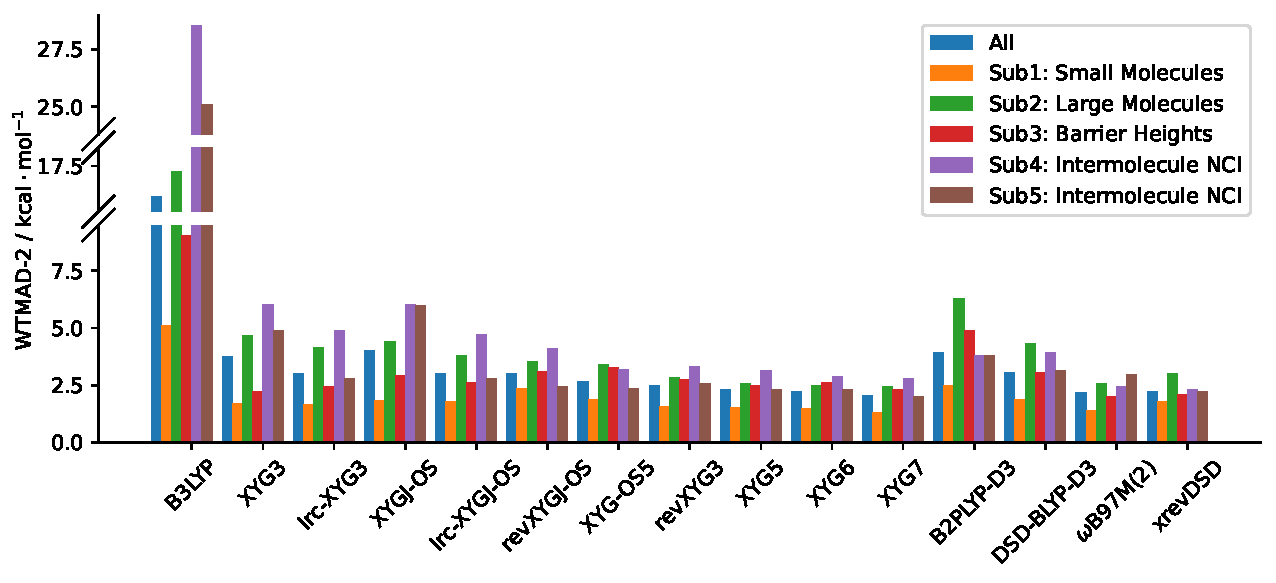
\includegraphics[width=0.8\textwidth]{assets/xdh-b3lyp-wtmad.pdf}
  \caption[双杂化泛函对 GMTKN55 数据集的测评]{各类双杂化密度泛函与 B3LYP 杂化泛函在 GMTKN55 数据集上的 WTMAD-2 测评表现。数据取自文献\cite{Zhang-Xu.JPCL.2021}。图表样式参考论文\cite{Yan.Thesis.2022}。下图中的 xrevDSD 泛函指代 xrevDSD-PBEP86-D4。}
  \label{fig.1.xdh-b3lyp-wtmad}
\end{figure}

\textbf{固体能量测评表现}。图 \ref{fig.1.xdh-solid} 中,王艺臻、李亚静等对 XYG3、XYGJ-OS 双杂化泛函、以及部分低阶 (2--4 阶) 泛函作分子解离能与固体聚合能的测评\cite{Wang-Xu.JA.2021}。其中,CE14 测试集包括 14 种具有强聚合能 (包括强共价键与离子键) 的固体,Bond142 测试集则是由 142 个小分子的键解离能。测评结果表明。尽管 SCAN 与 SCAN0 在处理固体聚合能上有不亚于 xDH 的测评结果,但在分子键能问题上则没有很好的表现。XYG3 与 XYGJ-OS 可以相比于其他低阶泛函、或波函数理论下的 MP2 与 RPA 方法,能够更好地同时处理固体与分子体系中强共价作用的问题,取得两家之长。该工作的其它测评表明,XYGJ-OS 在金红石的两相结构、一氧化碳分子在氯化钠晶体下的吸附能等典型固体计算问题下也有优异的表现。

\begin{figure}[h]
  \centering
  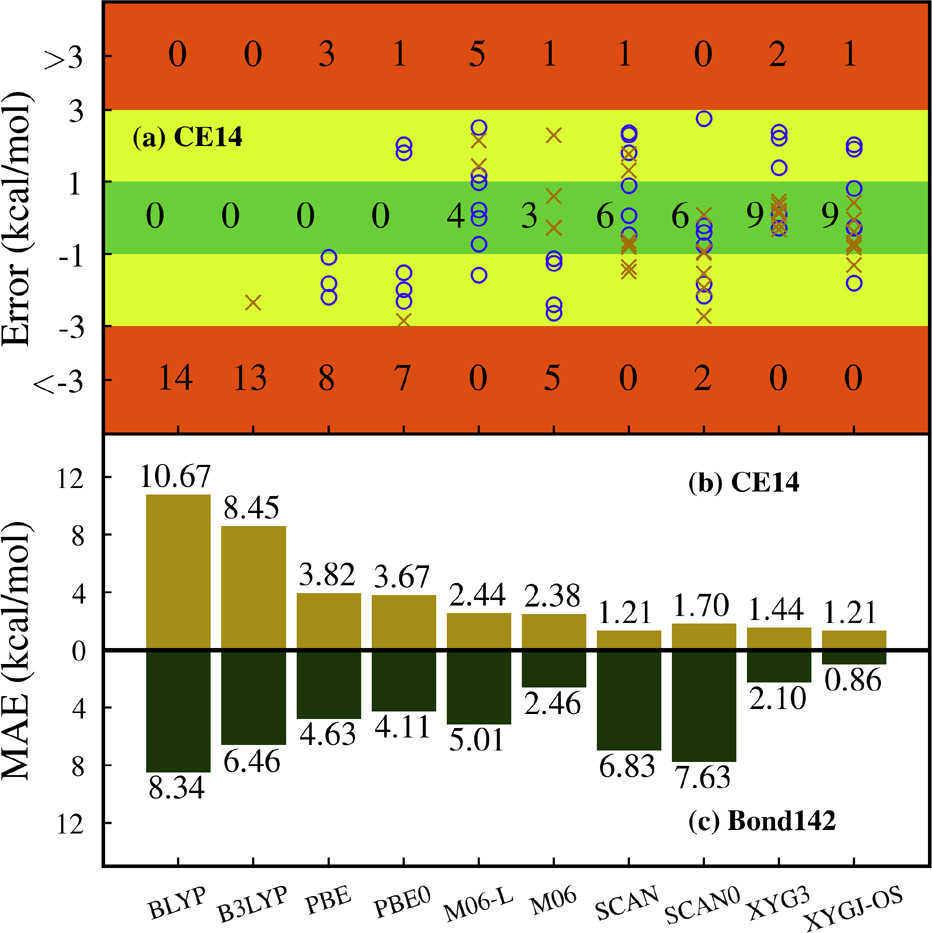
\includegraphics[width=0.4\textwidth]{assets/xdh-solid.jpeg}
  \caption[泛函近似对固体聚合能与分子键解离能问题的测评]{固体聚合能测试集 CE14 与分子键解离能测试集 Bond142 测评结果。CE14 呈现的是分摊到每个原子上的误差表现。图片取自文献\cite{Wang-Xu.JA.2021}。}
  \label{fig.1.xdh-solid}
\end{figure}

\textbf{分子几何结构}。图 \ref{fig.1.xdh-pbe0-bond} 中,苏乃强等对包括 xDH 型双杂化泛函的部分杂化、双杂化泛函作分子几何结构的测评\cite{Su-Xu.SCC.2013}。为了方便比较测评结果,选取了缩放的 s-MAD (即以 XYG3 为单位测评结果作为 1 进行缩放的平均绝对值误差) 作为测评依据。其中,Cov 测试集包括 63 种共价分子与离子体系、NBI 测试集选用了 6 种小分子的二聚体结构用于测评非共价相互作用下的键长表现、TS 测试集收录了 12 个过渡态结构信息。可以看到,作为“Jacob 阶梯”第 5 阶的双杂化泛函的总体表现明显优于第 4 阶的 B3LYP 与 PBE0。除了 xDH-PBE0 在非键作用体系有待改进外,xDH 型泛函在各个数据集上的表现也明显优于 B2PLYP 或 MP2。

\begin{figure}[h]
  \centering
  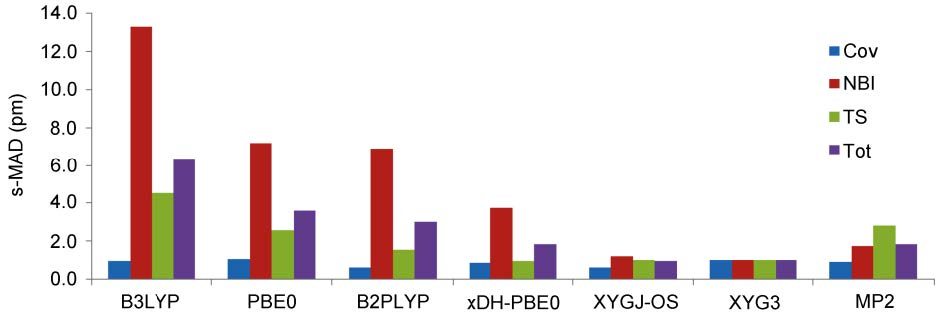
\includegraphics[width=0.7\textwidth]{assets/xdh-pbe0-bond.jpg}
  \caption[泛函近似对分子构型问题的测评]{部分杂化、双杂化泛函及 MP2 方法在分子结构上的总体表现。Cov 代表共价键合分子、NBI 代表非键作用体系、TS 代表过渡态结构、Tot 代表三者的平均。图片取自文献\cite{Su-Xu.SCC.2013}。}
  \label{fig.1.xdh-pbe0-bond}
\end{figure}

\textbf{振动频率}。表 \ref{tab.1.xdh-freq-bench} 中,谷永浩等对部分泛函的谐振频率作测评\cite{Gu-Xu.JCTC.2021}。测试集 F38 包含 38 个小分子的高精度谐振频率实验测量结果 (除 \ce{NH3} 的伞式振动参考值为 CCSD(T)/cc-pVQZ 计算结果)。XYGJ-OS、B2PLYP、xDH-PBE0 的测评表现较好,与实验结果的误差平均不超过 30 $\text{cm}^{-1}$。与此同时,XYGJ-OS 的误差分布较窄,产生较大误差的分子很少。对比 xDH 中表现较好的泛函 XYGJ-OS 与 xDH-PBE0、与其基底泛函 B3LYP 与 PBE0,可以认为在频率计算问题中,泛函的精度仍然沿着“Jacob 阶梯”的爬升稳步提高。

\begin{table}[h]
\centering
\caption[泛函近似对分子谐振频率问题的测评]{部分泛函在 F38 测试集下谐振频率计算的测评表现。误差单位为波数 ($\text{cm}^{-1}$)。数据取自文献\cite{Gu-Xu.JCTC.2021}。}
\label{tab.1.xdh-freq-bench}
\widetabular{
  \begin{tabular}{l
      S[table-format=+3.1]
      S[table-format=+3.1]
      S[table-format=+3.1]
      S[table-format=+3.1]
      S[table-format=+3.1]
      S[table-format=+3.1]}
    \toprule
        & {XYG3} & {XYGJ-OS} & {xDH-PBE0} & {B2PLYP} & {B3LYP} & {PBE0} \\
    \midrule
    MAD & 42   & 19      & 28       & 18     & 33    & 42   \\
    MIN & -87  & -65     & -105     & -51    & -75   & -55  \\
    MAX & 115  & 42      & 51       & 96     & 130   & 122  \\
    误差范围 & 202 & 107 & 156 & 147 & 205 & 177 \\
    \bottomrule
  \end{tabular}
}{}
\end{table}

\textbf{核磁屏蔽常数}。图 \ref{fig.1.xdh-nmr} 中,颜文杰等对部分双杂化泛函的核磁屏蔽常数作测评\cite{Yan-Xu.JCTC.2022}。FPA-M 数据集包含 20 个分子的 34 个 \ce{^{13}C}、\ce{^{15}N}、\ce{^{17}O}、\ce{^{19}F} 原子核的化学位移理论计算结果;其参考值是 FPA 模型下的 CCSD(T)/CBS 结果。测评表明,XYGJ-OS 在诸多双杂化泛函中有出色的表现,并且误差明显小于 Stoychev 等的测评文章\cite{Stoychev-Neese.JCTC.2018} 中表现最好的 DSD-PBEP86 泛函。该工作同时测评了氢原子的化学位移,表明 XYGJ-OS 与 xDH-PBE0 等泛函在 HC\_48/40 数据集上的测评精度对于 \ce{^{1}H} 而言约为 0.03 ppm、对于 \ce{^{13}C} 而言约为 1 ppm,达到了相当高的精度。

\begin{figure}[h]
  \centering
  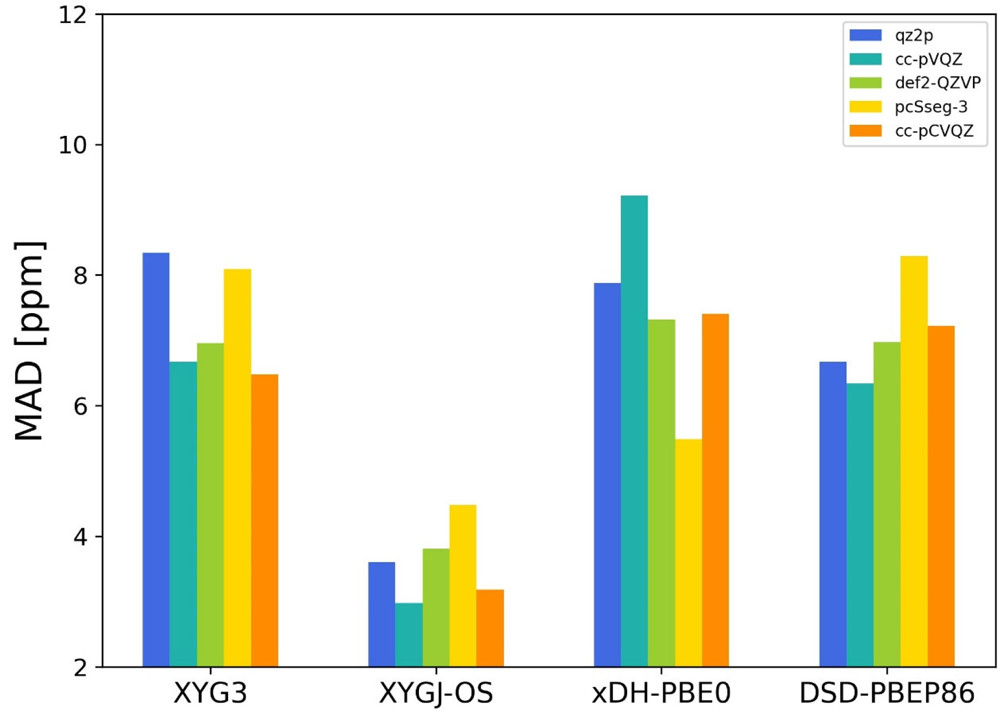
\includegraphics[width=0.4\textwidth]{assets/xdh-nmr.jpeg}
  \caption[泛函近似对 NMR 屏蔽常数问题的测评]{部分双杂化泛函在 FPA-M 集上以 4-$\zeta$ 基组计算的 NMR 屏蔽常数测评表现。图片取自文献\cite{Yan-Xu.JCTC.2022}。}
  \label{fig.1.xdh-nmr}
\end{figure}

\section{本文研究思路与主要工作}

xDH 型泛函构造的理论框架搭建在绝热路径与 G\"{o}rling-Levy 微扰之上,使用较好的单电子轨道作为基础,并在能量计算中追求“Jacob 阶梯”上更高、更精确的阶梯,有着良好的理论基础。xDH 型双杂化泛函在分子能量与性质计算上,其精度水平代表了目前密度泛函方法的最高水准。对于类如 MP2 与 RPA 等相近计算量或计算标度的 post-SCF 方法而言,双杂化泛函的精度通常也更为优异。近年来发展的 xDH 泛函在主族化学反应的能量的表现,已经在切实地逼近 1 kcal/mol 的化学精度;而其它性质的测评工作也表明,xDH 型泛函不仅在能量,还在分子几何结构、振动频率、核磁屏蔽常数等问题上有令人鼓舞的表现。而这些良好的数值结果,也印证了 xDH 型泛函良好的理论框架的重要性。但也需要指出,目前发展的大多数 xDH 型泛函近似的具体实现,依赖于 (Generalized) Kohn-Sham 框架导出的轨道、以及 MP2 型相关能;这两者存在的问题,也可能会反映到 xDH 型双杂化泛函、以及作为退化形式的 bDH 型双杂化泛函的测评表现中。

除了精度上双杂化泛函仍然有发展空间外,其在应用的推广也是重要的课题。在双杂化泛函刚提出的 2004--2010 年代,由于大多数计算化学软件在处理 MP2 型相关能时的计算量很大;即使测评结果较好,也难以推广到实际的应用中。随着一系列针对相关能以及双电子积分计算近似方法、算法与程序的发展,在处理 20 原子以下的分子体系时,MP2 相关能的计算耗时经常少于自洽场的计算耗时,使得双杂化泛函在能量计算问题上不再有严重的效率瓶颈。而对于更大的计算体系,ONIOM 或 XO 等组合化学方法通常可以有效地拆分问题而不严重影响计算精度\cite{Guo-Xu.JCC.2012, Chen-Xu.JCTC.2020, Chen-Xu.NC.2023}。因此,在可见的未来内,在分子体系的计算问题上,双杂化密度泛函的主要应用会集中在数十个原子左右尺度的问题上。

基于以上的研究思路和认识,本文的主要工作从以下五个方面展开。
\begin{enumerate}[nosep]
  \item \textbf{基于成对电子方法的双杂化能量泛函实现与测评。}(第 \alertref{sec.2.title} 章) MP2 型相关能在处理分子解离曲线、过渡金属体系等涉及 Kohn-Sham 轨道能级近简并问题时,容易导致及其严重的误差。为减小近简并体系误差的严重性,双杂化泛函中需要考虑引入其它形式的相关能。基于 G\"orling-Levy 微扰所构建的密度泛函与波函数理论的桥梁,本工作尝试在双杂化泛函中,引入以波函数理论中对 MP2 相关能矫正方法 MP2/cr\cite{Dykstra-Davidson.IJQC.2000} 为代表的成对电子型相关能。我们将构建新的泛函参数化模型,并对参数作系统的优化,考察该类型泛函在一般双杂化泛函表现优异的主族化学反应、与表现欠佳的多参考体系和解离分子体系下的表现。我们期望这份工作,在双杂化近似的框架下,向真实泛函迈进一小步。

  \item \textbf{双杂化泛函的电性质梯度理论与程序实现。}(附录 \alertref{sec.3.title}) 许多分子的性质,譬如分子频率、偶极矩与极化率、化学屏蔽常数、弛豫密度等都需要基于梯度理论得以计算实现。xDH 型泛函的一阶梯度与二阶梯度已经分别由苏乃强等\cite{Su-Xu.SCC.2013}与谷永浩等\cite{Gu-Xu.JCTC.2021}提出。作为本工作中后三章内容的程序实现基础,在电性质外场为微扰的前提下,对 DH 的梯度理论作回顾。除此之外,本工作将尝试扩充该梯度理论到更为一般的非变分双杂化泛函框架,为将来在同一程序框架下实现多种形式的双杂化泛函能量与梯度性质作准备。最后,作为该框架的具体应用,我们将基于开源框架 \textsc{PySCF} 发展扩展程序 \textsc{dh},实现 RI 近似下包含 MP2 型相关能的 DH 极化率,以扩展目前 DH 在分子性质上的算力到 2000 以上基函数的级别。这部分工作仅程序实现是独立完成的工作;理论部分是前人工作的重新推演与整理,{\color{red}\textbf{并非独创性工作}},且由于较为冗长,因此置于附录。
  
  \item \textbf{双杂化泛函原子体系电子云密度与能量测评。}(第 \alertref{sec.4.title} 章) Medvedev 等指出,在非常基本的原子体系能量与密度计算问题上,密度泛函近似并没有随着提出的年代愈近有更好的表现\cite{Medvedev-Lyssenko.S.2017};这让该文章作者产生了“密度泛函是否偏离了逼近真实泛函的道路上”的疑问。他们同时指出,表现欠佳的泛函的共性是含有重度的参数拟合、以及没有建立在合理的理论模型之上或泛函近似在“Jacob 阶梯”的阶数较低。本工作在 Medvedev 等人的测评基础上,对诸多双杂化泛函进行原子能量与密度的计算测评。我们将探究以 xDH 型泛函为代表的双杂化泛函,作为少或无拟合参数、且不专门针对原子体系进行优化的泛函,是否有着相当良好的测评表现;以及随着密度泛函近似的“Jacob 阶梯”的提升,密度泛函是否在原子体系问题下精度有精度的改善。
  
  \item \textbf{高精度基组外推方法在 CCSD(T) 静态极化率计算上的应用。}(第 \alertref{sec.5.title} 章) 该部分工作是第 \alertref{sec.6.title} 章测评双杂化泛函静态极化率的前置工作。静态极化率是描述光学性质与分子间相互作用等问题的重要物理量。一般来说,静态极化率的实验精度误差为 0.5\% 左右;但目前大多数测评数据集的参考值在计算方法或基组上,都与该精度级别有一定差距。有赖于当前高效率的双杂化泛函的极化率程序,大基组的 MP2 极化率对计算资源的消耗已比较小;但可以作为极化率参考值计算方法的 CCSD(T) 计算消耗仍然巨大。FPA 方法是一种波函数理论的组合方法;在我们的工作中,它将大基组的 MP2 计算结果与中等基组大小的 CCSD(T) 相关能结果结合起来,从而以较低的计算代价实现高精度的极化率计算。本工作将系统地测评各级别 FPA 方法的误差,并将 FPA 方法应用到现有的极化率数据集,以提升数据集精度。
  
  \item \textbf{双杂化泛函的静态极化率测评。}(第 \alertref{sec.6.title} 章) 本工作对目前流行的 MP2 型双杂化泛函作系统性的静态极化率测评。该测评的结果将表明,xDH 型泛函在无机与有机、自旋极化与非极化、小分子与中等分子等各类体系下,都有非常良好的极化率表现。该工作也尝试从长短程分离、自旋相同与相反、泛函拟合参数等方面切入,考察这些效应对双杂化泛函在极化率测评表现上的影响。
  
\end{enumerate}
从章节编排上,摘要的介绍顺序是程序与数据集等基础的发展 (附录 \alertref{sec.3.title}、第 \alertref{sec.5.title} 章),泛函开发 (第 \alertref{sec.2.title} 章),泛函测评 (第 \alertref{sec.4.title}、\alertref{sec.6.title} 章)。正文的介绍顺序是能量计算问题 (第 \alertref{sec.2.title} 章),作为第 \alertref{sec.4.title}、\alertref{sec.5.title}、\alertref{sec.6.title} 章的技术支撑的程序开发 (附录 \alertref{sec.3.title}),作为一阶性质的电子云密度测评 (第 \alertref{sec.4.title} 章),作为第 \alertref{sec.6.title} 章的参考值支撑的高精度组合方法开发 (第 \alertref{sec.5.title}),作为二阶性质的极化率测评 (第 \alertref{sec.6.title} 章)。

\newpage



\graphicspath{{../chap-02/}}
% !TEX root=./dummy-02.tex

\chapter{基于对电子方法的双杂化能量泛函实现与测评}
\label{sec.2.title}

\section{引言}

分子体系的基态能量始终是计算化学所关心的根本问题。只有准确地描述分子基态能量,才有可能准确描述分子自由能等热力学性质,并进而将计算结果应用于反应动力学、分子动力学、精细光谱等各种具体的化学或物理问题。目前主流的对分子体系基态性质描述的理论体系,有 post-HF、DFT、QMC 等。由于 DFT 的近似方法相比于其它理论框架下的方法而言,在相同的计算资源消耗下,可以对更大的分子体系作计算、并有更高的精度,即计算消耗与精度的性价比高;因此,密度泛函近似在计算化学应用受到广泛的欢迎与使用。在第 \alertref{sec.1.title} 章中,也回顾到密度泛函近似的其中一个分支,双杂化泛函,在涉及主族化学的各类反应能量、弱相互作用、几何结构、分子振动与谱学问题有良好的表现。

但密度泛函近似仍然存在一些困难。目前主流的密度泛函可以依据开发模式分为两类:经验参数拟合的、与纯理论模型的。一般来说,纯理论模型的泛函在测评数据集上的表现通常稍逊色\cite{Goerigk-Grimme.PCCP.2017};但对于经验参数拟合的泛函,可能在拟合范围外产生比较严重误差,即可泛化性通常较差\cite{Medvedev-Lyssenko.S.2017}。目前流行的大多数双杂化泛函,为保证一定的泛化能力,可以采用的策略是使用较少的参数数量,如 XYG$n$\cite{Zhang-Xu.JPCL.2021} 或 DSD 系列\cite{Kozuch-Martin.JCC.2013}等泛函;或者采用复杂的参数拟合策略,如 ωB97X-2\cite{Chai-Head-Gordon.JCP.2009} 或 ωB97M(2)\cite{Mardirossian-Head-Gordon.JCP.2018}等泛函。这些泛函的参数通常是针对主族化学体系的反应能与弱相互作用能数据集上拟合得到;但目前的测评中,这些泛函确实在原子密度\cite{Su-Xu.PNAS.2018}、偶极矩与极化率\cite{Hait-Head-Gordon.JCTC.2018, Hait-Head-Gordon.PCCP.2018}、化学位移\cite{Stoychev-Neese.JCTC.2018}等问题上有良好的结果,即表现出不错的泛化能力。但同时需要注意到,这些泛函仍然在以过渡金属体系,以及具有静态相关或分数电荷与自旋特性的体系为代表的一些计算问题上,数值表现通常还有提升的空间\cite{Cohen-Yang.S.2008, Mori-Sanchez-Yang.PRL.2009, Hesselmann-Goerling.PRL.2011, Cohen-Yang.CR.2012, Zhang-Scheffler.PRL.2016,Zhang-Xu.JPCL.2021}。

目前流行的双杂化泛函,通常是对基于 Kohn-Sham 参考态的电子云分布,引入 MP2 型相关能 $E_\textmt{c}^\textmt{MP2}$。若分子体系的 HOMO/LUMO gap 较小,则 $E_\textmt{c}^\textmt{MP2}$ 会产生严重的负误差。由于一部分过渡金属与多参考问题具有 HOMO/LUMO gap 较小的特性,因此双杂化泛函在这类问题上表现较差。波函数理论中,与 MP2 计算量相仿的电子对方法 IEPA\cite{Sinanoǧlu-Sinanoǧlu.ACP.1964, Nesbet-Nesbet.ACP.1965}、sIEPA\cite{Zhang-Scheffler.PRL.2016}、MP2/cr\cite{Dykstra-Davidson.IJQC.2000}\footnote{在 Dykstra and Davidson 原文\cite{Dykstra-Davidson.IJQC.2000}中提出了两种 MP2/cr 形式。原文的 MP2/cr-II 的计算需要自旋相同且同占据轨道角标的激发系数 $t_{i \bar i}^{a \bar b}$;这在 $\alpha, \beta$ 占据数不同的情形下难以合理地定义。在正文中,我们仅介绍与使用原文的 MP2/cr-I,并将其指代为 MP2/cr。} 等可以一定程度地避免 $E_\textmt{c}^\textmt{MP2}$ 型相关能的负误差。在双杂化泛函中引入这类相关能,有望在不加大计算量的同时,提高 HOMO/LUMO gap 较小体系问题的计算精度。这三类近似方法在本工作中统称为 EP 型相关能。

在理论层面,掺杂 MP2 型相关能的双杂化泛函基础,一般认为是 G\"orling-Levy 微扰理论的二阶近似。事实上,G\"orling-Levy 微扰理论建立起了密度泛函方法与波函数理论之间的联系,而这层联系不仅仅局限于二阶微扰、还可以与更高级的方法产生联系。从这个角度来看,在密度泛函中引入不同于 MP2 的其它波函数理论下的相关能,在 G\"orling-Levy 微扰理论的角度下是可以立足的。

基于这些认识,在本章工作中,将实现掺杂 EP 型相关能的双杂化泛函,并进行理论合理性说明与测评。\ref{sec.2.glpt2-theory}--\ref{sec.2.glpt2-dh} 小节将回顾 G\"orling-Levy 微扰理论,进一步详细地阐述其与波函数理论之间的关系,以及在密度泛函近似中引入波函数方法相关能的合理性。\ref{sec.3.ep} 节将回顾作为波函数理论的 EP 型相关能近似理论与计算实现。\ref{sec.2.iepa-results} 节将通过参数拟合的方式给出掺杂 EP 型相关能的双杂化泛函,并对部分主族化学、过渡金属体系、多参考问题进行测评,以及对参数优化过程进行讨论。

\section{理论背景}

\subsection{GLPT2 的理论框架}
\label{sec.2.glpt2-theory}

目前的双杂化泛函,大多数选用 GLPT2 作为其理论框架的支撑依据。我们也将使用 GLPT2 作为理论基础,并对此作简要的讨论。

密度泛函理论,相比于波函数理论,通常被认为可以以更低的计算代价实现较为准确的计算;但普适泛函 $F[\rho]$ 的获得途径并不清晰,因此如何系统性地逼近真实泛函,成为密度泛函发展的瓶颈之一。

对于易于求得、但需要借助于确切值的普适泛函 $F[\rho]$ 的 Kohn-Sham 波函数,与计算量巨大、但可以严格逼近确切值求得的真实波函数,绝热路径理论可以通过耦合常数 $\lambda$ 将两种波函数联系起来。该耦合常数 $\lambda$,以及其对应的 Hamiltonian 量定义如下:
\begin{equation}
  \label{eq.2.H-lambda-ac}
  \hat H_\lambda = \hat T + \lambda \hat V_\mathrm{ee} + \sum_i^{n_\mathrm{elec}} v_{\lambda}(\bm{r}_i)
\end{equation}
其中,$v_{\lambda}(\bm{r})$ 是随耦合常数 $\lambda$ 改变而不同的势函数;其作用是用于保持在不同的 $\lambda$ 下,$\hat H_\lambda$ 所给出的波函数的密度都等同于真实体系密度 $\rho(\bm{r})$。

如同波函数理论从 Hartree-Fock 波函数出发,经过微扰处理可以得到精确波函数;依耦合常数 $\lambda$ 展开的绝热路径上的微扰,也可以得到精确波函数;后者也称为 G\"orling-Levy 微扰框架\cite{Goerling-Levy.PRB.1993, Goerling-Levy.PRA.1994}。在该微扰框架下,定义 $\hat H_\lambda$ 对应的本征态为 $| \Psi_\lambda \rangle$;作为特例,真实波函数为 $| \Psi_{\lambda = 1} \rangle$,Kohn-Sham 波函数为 $| \Psi_{\lambda = 0} \rangle$;这两个波函数成功地通过耦合常数 $\lambda$ 得以联系。定义绝热路径上的被积函数
\begin{align}
  \label{eq.2.adiabatic-curve-w}
  \mathcal{W}_{\lambda} [\rho] &= \langle \Psi_\lambda | \hat V_\mathrm{ee} | \Psi_\lambda \rangle \\
  \mathcal{W}_{\textmt{c}, \lambda} [\rho] &= \mathcal{W}_{\lambda} [\rho] - E_\textmt{x}^\textmt{exact} [\rho] = \mathcal{W}_{\lambda} [\rho] - \langle \Psi_{\lambda = 0} | \hat V_\mathrm{ee} | \Psi_{\lambda = 0} \rangle
\end{align}
则普适泛函 $F[\rho]$ 中,唯一无法由 Kohn-Sham 波函数简单给出的相关能 $E_\textmt{c} [\rho] = E_{\textmt{c}, \lambda=1} [\rho]$,则由 Hellmann-Feynman 定理,可以展开为对耦合常数 $\lambda$ 的积分
\begin{equation}
  E_{\textmt{c}, \lambda} [\rho] = \int_0^\lambda \mathcal{W}_{\textmt{c}, \lambda} [\rho] \, \mathrm{d} \bm{r}
\end{equation}

假使 $E_{\textmt{c}, \lambda} [\rho]$ 在以 $\lambda=0$ 为中心的邻域 $(0, 1]$ 下 Taylor 级数收敛,那么我们用下述记号表示该 Taylor 展开:
\begin{equation}
  \label{eq.2.e-c-lambda}
  E_{\textmt{c}, \lambda} [\rho] = \sum_{n=2}^{\infty} \lambda^n E_\textmt{GL}^{(n)} [\rho]
\end{equation}
作为具体的结果,G\"orling-Levy 微扰展开到第二阶时,其能量 $E_\textmt{GL}^{(2)}$ 具有较为简单的形式:
\begin{align}
  \label{eq.2.GL2-W}
  E_\textmt{GL}^{(2)} &= \frac{1}{2} \lim_{\lambda \rightarrow 0} \frac{\mathrm{d}^2}{\mathrm{d}^2 \lambda} E_{\textmt{c}, \lambda} [\rho] = \frac{1}{2} \lim_{\lambda \rightarrow 0} \frac{\mathrm{d}}{\mathrm{d} \lambda} \mathcal{W}_{\textmt{c}, \lambda} [\rho] \\
  \label{eq.2.GL2-def}
  &= \sum_{ia} \frac{\big| \langle i | \hat v_\textmt{x}^\textmt{NL} - v_\textmt{x} | a \rangle \big|^2}{\varepsilon_i - \varepsilon_a} + \frac{1}{4} \sum_{ijab} \frac{\big| \langle ij || ab \rangle \big|^2}{\varepsilon_i + \varepsilon_j - \varepsilon_a - \varepsilon_b}
\end{align}
上式的 $v_\textmt{x}^\textmt{NL}$ 是非局域交换势算符。

对于式 (\ref{eq.2.GL2-W}),从更直观的角度来看,$\mathcal{W}_{\textmt{c}, \lambda} [\rho]$ 作为关于 $\lambda$ 的函数,其在 $\lambda = 0$ 处的曲线斜率恰是 $2 E_\textmt{GL}^{(2)}$;同时参考图 \ref{fig.2.adiabatic-curve}。而若进一步假设曲线 $\mathcal{W}_{\textmt{c}, \lambda} [\rho]$ 关于 $\lambda$ 近似为直线,那么相关能就可以近似为 GLPT2 微扰能,即 $E_\textmt{c} [\rho] \simeq E_\textmt{GL}^{(2)}$。

\begin{figure}[h]
  \centering
  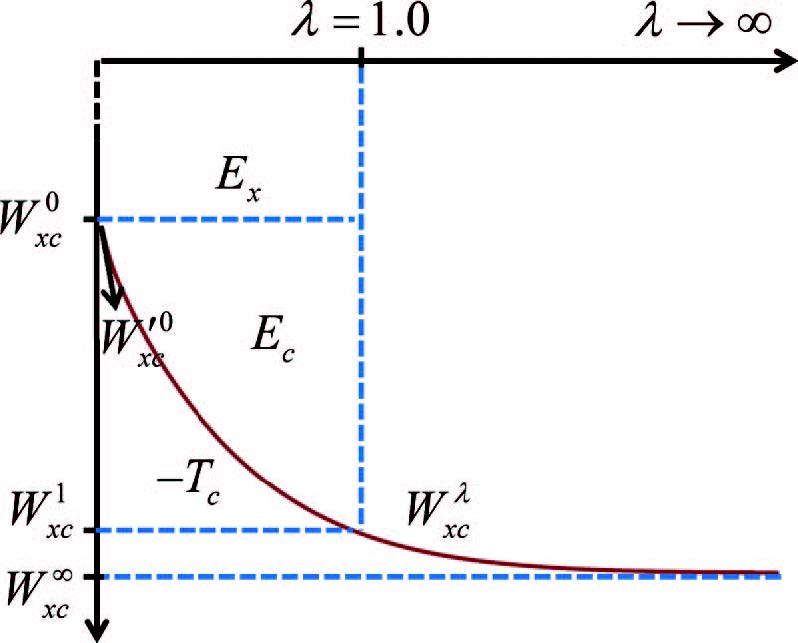
\includegraphics[width=0.5\textwidth]{assets/adiabatic-curve.jpg}
  \caption[绝热路径曲线示意图]{绝热路径曲线示意图。下图取自文献\cite{Su-Xu.JCP.2014}。图中的 $W_{xc}^{\lambda}$ 即本文中的 $\mathcal{W}_{\lambda}$。图中的 $W'_{xc}{}^{0}$ 数值上等于本文中的 $2 E_\textmt{GL}^{(2)}$。}
  \label{fig.2.adiabatic-curve}
\end{figure}

而对于式 (\ref{eq.2.GL2-def}),尽管 $E_\textmt{GL}^{(2)}$ 的表达式相比于 MP2 相关能 $E_\textmt{c}^\textmt{MP2}$ 多出了关于 $v_\textmt{x}^\textmt{NL}$ 的单电子贡献项;但一般来说单电子贡献非常小\cite{DellaSala-Goerling.JCP.2001},同时 $v_\textmt{x}$ 在实际计算中需要代价昂贵的响应函数方法\cite{Goerling-Goerling.PRL.1999}、或存在数值不稳定可能性的 KLI 方法\cite{Krieger-Iafrate.PRA.1992, DellaSala-Goerling.JCP.2001}或 OEP 方法\cite{Mori-Sanchez-Yang.JCP.2005};因此忽略上式的第一项,即单电子项,通常是可接受的。从而,$E_\textmt{GL}^{(2)}$ 可以仅由第二项近似得到:
\begin{equation}
  E_\textmt{GL}^{(2)} \simeq E_\textmt{c}^\textmt{MP2}
\end{equation}
这里 $E_\textmt{c}^\textmt{MP2}$ 是指基于 Kohn-Sham 波函数所给出的 MP2 相关能。

\subsection{GLPT2 与双杂化泛函}
\label{sec.2.glpt2-dh}

现在回到近似泛函的问题上。上一小节通过分析给出了 Kohn-Sham 相关能泛函与 MP2 相关能,在 $\mathcal{W}_{\textmt{c}, \lambda} [\rho]$ 关于 $\lambda$ 接近线性、以及 $\hat v_\textmt{x}^\textmt{NL} - v_\textmt{x}$ 算符效果接近于零的假设下,是非常相似的结论;即 $E_\textmt{c} [\rho] \simeq E_\textmt{GL}^{(2)} \simeq E_\textmt{c}^\textmt{MP2}$。当然现实情况下,$\mathcal{W}_{\textmt{c}, \lambda} [\rho]$ 关于 $\lambda$ 并非严格线性,因此上述近似一般不能直接使用;但将 $E_\textmt{c}^\textmt{MP2}$ 作为杂化项掺入泛函,仍然是有所帮助的。这就构成了一般的 MP2 型双杂化泛函。但 MP2 相关能仅仅是最初步的其中一种引入 G\"orling-Levy 微扰方式;从具体实现上,如何引入 G\"orling-Levy 微扰、引入多大程度的近似能得到较精确地结果,都是值得讨论的话题。

理论上,我们可以获得依式 (\ref{eq.2.e-c-lambda}) 定义的 $\lambda=0$ 处各阶微扰能量;从而在 $\lambda$ 的级数收敛区间内给出最终的 $E_{\textmt{c}, \lambda} [\rho]$。显然,若可以求得更高阶数的 G\"orling-Levy 微扰能 $E_\textmt{GL}^{(n)}$ ($n > 2$),那么相关能的结果就更为精确。但如果对 G\"orling-Levy 微扰作更多分析,那么算符 $\hat H_\lambda$ 对耦合常数 $\lambda$ 的展开表达式为
\begin{equation}
  \hat H_\lambda = \left( \hat T - \sum_i^{n_\mathrm{elec}} v_\mathrm{s} (\bm{r}_i) \right) + \lambda \left( \hat V_\mathrm{ee} - \sum_i^{n_\mathrm{elec}} \big( v_\mathrm{J} (\bm{r}_i) + v_\textmt{x} (\bm{r}_i) \big) \right) - \sum_{n=2}^\infty \lambda^n \sum_{i}^{n_\mathrm{elec}} v_\textmt{c}^{(n)} (\bm{r}_i)
\end{equation}
其中,上式中出现的势函数是一些能量项对密度的函数变分:
\begin{equation*}
  v_\mathrm{s} (\bm{r}) = \frac{\delta T_\mathrm{s} [\rho]}{\delta \rho(\bm{r})} , \;
  v_\mathrm{J} (\bm{r}) = \frac{\delta J [\rho]}{\delta \rho(\bm{r})}, \;
  v_\textmt{x} (\bm{r}) = \frac{\delta E_\textmt{x}^\textmt{exact} [\rho]}{\delta \rho(\bm{r})}, \;
  v_\textmt{c}^{(n)} (\bm{r}) = \frac{\delta E_\textmt{GL}^{(n)} [\rho]}{\delta \rho (\bm{r})}
\end{equation*}
由于在算符 $\hat H_\lambda$ 中存在算符 $\hat V_\mathrm{ee}$,因此,$n$ 阶的 G\"orling-Levy 计算量至少不会低于 M\o{}ller-Plesset 对应 $n$ 阶的微扰。

可以预见,G\"orling-Levy 微扰的计算代价是相当高的。但也需要指出,由于近年来近似算法 (特别是 RI 近似算法)、以及计算硬件 (特别是 DRAM 内存容量) 发展,MP2 相关能的计算在数十原子体系以内耗时不多于引入交换效应的 Kohn-Sham 自洽场计算;因此,对于 $n = 2$ 阶 G\"orling-Levy 微扰即 GLPT2,若近似为 MP2 相关则不会增加太多计算资源负担。而对于 $n = 3$ 阶的情形,现在确实有针对 MP3 相关能的计算所提出或适用的近似算法;这类算法通常基于 THC 或其它张量分解与缩并方法\cite{Hohenstein-Martinez.JCP.2012, Parrish-Sherrill.JCP.2012, Lee-Head-Gordon.JCTC.2020, Matthews-Matthews.JCTC.2020},但目前的效率仍然无法达到与自洽场计算齐平的程度\cite{Matthews-Matthews.JCP.2021}。考虑到杂化密度泛函近似近年来的巨大成功,得益于可以在较低自洽场级别的计算代价下获得相对精确的结果;其中计算代价小是非常重要的因素。因此,若 MP3 相关能的计算效率难以进一步提升,那么在可见的未来,基于 G\"orling-Levy 微扰理论所开发的实用的密度泛函,很可能不会引入\textbf{完整的} $n = 3$ 阶或更高阶微扰能量。

因此,若以 G\"orling-Levy 为基础发展泛函方法,仅引入 GLPT2 从计算资源消耗与精度平衡的角度上,是非常自然的想法。作为最基本的泛函模型,$\mathcal{W}_{\lambda}$ 若依 $\lambda$ 接近线性,则
\begin{equation}
  E_{\textmt{xc}, \lambda} [\rho] = \lambda E_\textmt{x}^\textmt{exact}[\rho] + \lambda^2 E_\textmt{GL}^{(2)} [\rho] + o(\lambda^3) \simeq E_\textmt{x}^\textmt{exact}[\rho] + E_\textmt{GL}^{(2)} [\rho]
\end{equation}
当 $\lambda = 1$ 时,上述的 $E_{\textmt{xc}, \lambda} [\rho]$ 就是真实体系的交换相关能 $E_{\textmt{xc}} [\rho]$。但事实上,当相关能若仅引入 GLPT2 时,测评表现并不好\cite{Su-Xu.JCP.2014}。事实上,重新回顾式 (\ref{eq.2.GL2-W}) 的结论,微扰理论只能描述取到极限 $\lambda \rightarrow 0$ 时绝热路径曲线行为。若 $E_{\textmt{c}, \lambda} [\lambda]$ 作为关于 $\lambda$ 的函数在 $(0, 1]$ 邻域上 Taylor 级数收敛,那么精确地描述 $\lambda \rightarrow 0$ 处越热路径曲线的行为 (可以精确计算 $\lambda \rightarrow 0$ 的各阶导数),也能给出正确的 $\lambda \in (0, 1]$ 下 $\mathcal{W}_{\lambda}$ 的结果;从而对 $\mathcal{W}_{\lambda}$ 作关于 $\lambda$ 的积分得到准确的 $E_\textmt{xc}$。但在计算资源的限制下,如图 \ref{fig.2.adiabatic-curve} 所示,如果无法引入三阶或更高阶微扰能量,即只能相对精确地计算 $\mathcal{W}_{\lambda}$ 在 $\lambda = 0$ 处的函数值与斜率,我们只能得到非常粗糙的对 $\lambda = 0$ 附近 $\mathcal{W}_{\lambda}$ 的局部认识、而无法对整体形状有所把握;大多数分子的 $\mathcal{W}_{\lambda}$ 并不非常接近线性,那么若仅近似 $E_\textmt{c} [\rho] \simeq E_\textmt{GL}^{(2)} [\rho]$,自然无法给出好的测评表现。

为提升测评精度,也为了更好地对大多数类型分子的 $\mathcal{W}_{\lambda}$ 作合理建模以更好地逼近真实的 $E_\textmt{xc} [\rho]$,其中一种有效且理论上相对严格的策略,是结合 G\"orling-Levy 微扰与传统的低阶密度泛函近似,对 $\mathcal{W}_{\lambda}$ 作合理的参数化。尽管传统的低阶泛函\footnote{低阶泛函 (low-rung functional) 指在“Jacob 阶梯”的第四阶或以下,即杂化泛函或以下的泛函。后文也经常使用该称法。}未必能正确地描述 $\mathcal{W}_{\lambda}$ 在 $\lambda \rightarrow 0$ 时的行为,但却因为对 $\mathcal{W}_{\lambda}$ 在 $\lambda \in [0, 1]$ 整体有良好的描述,传统泛函的 $E_\textmt{xc} [\rho]$ 的结果通常相比于仅近似 $E_\textmt{c} [\rho] \simeq E_\textmt{GL}^{(2)} [\rho]$ 的 GLPT2 要更精确。如果在构造绝热路径曲线 $\mathcal{W}_{\lambda}$ 的过程中,在 $\lambda \rightarrow 0$ 时偏重 G\"orling-Levy 微扰理论、而在 $\lambda \rightarrow 1$ 时偏重传统泛函,那么可以取两者所长,获得比传统泛函近似或 GLPT2 更为精确的泛函。在这种新的泛函形式中,交换相关能同时有严格交换能 $E_\textmt{x}^\textmt{exact}$ 与二阶微扰相关能 $E_\textmt{GL}^{(2)}$ 的掺杂:
\begin{equation}
  E_\textmt{xc} = \int_0^\lambda \mathcal{W}_{\lambda} \, \mathrm{d} \lambda = E_\textmt{xc}^\textmt{low-rung} + c_\textmt{x} E_\textmt{x}^\textmt{exact} + c_\textmt{c} E_\textmt{GL}^{(2)}
\end{equation}
因此这类泛函近似成为双杂化泛函。

许多在测评结果上有优异表现的双杂化泛函,譬如 B2PLYP、XYG3 等,通过上述策略对将双杂化泛函近似合理化\cite{Grimme-Grimme.JCP.2006, Zhang-Goddard.PNAS.2009};但在实践中,则是直接对 $E_\textmt{xc} [\rho]$ 中的参数 $c_\textmt{x}, c_\textmt{c}$ 在数据集下作拟合,而没有直接构造 $\mathcal{W}_{\lambda}$ 本身。以 PBE-ACDH\cite{Su-Xu.JCP.2014} 为代表的一类泛函,则是使用参数或模型构造 $\mathcal{W}_{\lambda}$ 并对 $\lambda$ 作积分,得到 $E_\textmt{xc} [\rho]$。

需要指出,对绝热路径曲线 $\mathcal{W}_{\lambda}$ 作参数化或模型化后积分,从而在 $E_\textmt{xc}$ 中引入 GLPT2 相关能,是双杂化泛函的其中一种理论基础。以 PBE0-DH\cite{Toulouse-Adamo.JCP.2011} 为代表的双杂化泛函,其理论基础并非构建于 $\lambda = 0$ 的 Kohn-Sham 轨道行列式下 G\"orling-Levy 微扰,而是构建于 $0 < \lambda < 1$ 下杂化泛函轨道行列式下的二阶微扰基础上\cite{Sharkas-Savin.JCP.2011};该理论引入绝热路径给出相关能的方式,与 G\"orling-Levy 微扰有些许不同。

不论是使用绝热路径、还是使用杂化泛函波函数下的微扰理论,都可以构造出双杂化泛函。但与低阶泛函中纯粹以理论模型驱动所构造 PBE、TPSS、SCAN 或他们对应的杂化泛函,在诸多数据集下测评表现相对于同等级参数拟合方法仍然有不少优势\cite{Goerigk-Grimme.PCCP.2017, Medvedev-Lyssenko.S.2017}的情况不同,存在经验参数的双杂化泛函近似通常要比纯理论模型驱动构造的泛函有更优异的测评表现\cite{Mehta-Goerigk.PCCP.2018}。因此,理论模型通常在双杂化泛函中扮演的角色,很可能是对双杂化泛函的合理化。若要提升双杂化泛函的测评数值表现,参数优化非常重要。

但理论模型仍然可以指导双杂化密度泛函的发展。目前在数值计算上的迹象表明,对于绝大多数体系,绝热路径曲线是凸曲线\cite{Frydel-Burke.JCP.2000, Fuchs-Burke.JCP.2005, Teale-Helgaker.JCP.2009,Teale-Helgaker.JCP.2010, Carrascal-Burke.JPCM.2015} (但该结论目前没有对任意体系成立的确切证明\cite{Crisostomo-Burke.LMP.2023}):
\begin{equation}
  \frac{\mathrm{d}^2}{\mathrm{d} \lambda^2} \mathcal{W}_{\lambda} \geqslant 0, \quad \lambda \in [0, 1] \quad \text{(conjecture)}
\end{equation}
这意味着图 \ref{fig.2.adiabatic-curve} 所示的绝热路径曲线 $\mathcal{W}_\lambda$,数值上必然不小于以 $E_\textmt{x}^\textmt{exact}$ 为零点、以 $2 E_\textmt{GL}^{(2)}$ 为斜率的直线;进而对 $\mathcal{W}_\lambda$ 积分后,存在的关系式是
\begin{equation}
  E_\textmt{xc} \geqslant E_\textmt{x}^\textmt{exact} + E_\textmt{GL}^{(2)} \quad \text{(conjecture)}
\end{equation}
或者等价地,GLPT2 相关能相对于真实体系相关能必然有一定的负误差:
\begin{equation}
  E_\textmt{GL}^{(2)} \leqslant E_{\textmt{c}, \lambda=1} \quad \text{(conjecture)}
\end{equation}
作为具体的例子,在低阶密度泛函近似所给出的能量相对精确、且所给出的 Kohn-Sham 轨道足够精确的前提下,若要在能量计算中引入 GLPT2 相关能,那么对于下述泛函模型
\begin{equation*}
  E_\textmt{xc}^\textmt{DH} = c_\textmt{x} E_\textmt{x}^\textmt{exact} + c_\textmt{x}^\textmt{low-rung} E_\textmt{x}^\textmt{low-rung} + c_\textmt{c} E_\textmt{GL}^{(2)} + c_\textmt{c}^\textmt{low-rung} E_{\textmt{c}, \lambda=1}^\textmt{low-rung}
\end{equation*}
我们应当预期
\begin{equation*}
  c_\textmt{c} + c_\textmt{c}^\textmt{low-rung} \leqslant 1 \quad \text{(conjecture)}
\end{equation*}
事实上,在 xDH@B3LYP 模型下的诸多泛函的优化结果印证了这个结论\cite{Zhang-Xu.JPCL.2021}。因此,要求 $c_\textmt{c}, c_\textmt{c}^\textmt{low-rung}$ 等相关能参数之和小于 1,是其中一种引入 GLPT2 相关能以构造双杂化泛函的限制条件。

同时,G\"orling-Levy 微扰理论本身是类似于波函数方法、通过微扰阶数增加而逐步逼近真实泛函的理论框架;因为微扰阶数的增加会导致计算资源的巨量消耗,现在的密度泛函近似避免使用更高阶的 G\"orling-Levy 微扰相关能而仅考虑 GLPT2。但注意到波函数理论中存在一些近似方法:它们在 M\o{}ller-Plesset 微扰或耦合簇理论的框架下,基于较低阶的近似,引入一部分计算量较小的高阶贡献。对应于 MP2 的计算消耗,介于 MP2 到 CCSD 的经典波函数方法有 IEPA\cite{Sinanoǧlu-Sinanoǧlu.ACP.1964, Nesbet-Nesbet.ACP.1965}、MP2/cr\cite{Dykstra-Davidson.IJQC.2000}、CC2\cite{Christiansen-Joergensen.CPL.1995} 等。在下一节中,我们将会回顾 IEPA 与 MP2/cr 方法,并表明这类方法的相关能将大于 MP2 的相关能。由于 GLPT2 相关能通常近似为基于 Kohn-Sham 轨道行列式的 MP2 相关能,而 GLPT2 相关能相对于真实体系的相关能 $E_\mathrm{c, \lambda=1}$ 总是负误差;同时,由于 G\"orling-Levy 微扰中包含 $\hat V_\mathrm{ee}$ 算符,因而一部分表达式预期与 M\o{}ller-Plesset 微扰有着同样的结构,在能量计算中引入高阶的基于 Kohn-Sham 轨道行列式的 M\o{}ller-Plesset 微扰能量是合理的;因此,在双杂化泛函近似中引入 IEPA 或 MP2/cr 等相关能,预期一定程度上可以化解 GLPT2 的负误差,并且是理论上合理的。

\subsection{电子对方法}
\label{sec.3.ep}

本工作考虑的 IEPA 方法与 MP2/cr 方法,从计算过程而言,都是基于占据电子成对效应而实现;因此我们统称这两类方法为电子对或 EP 方法。在将这类电子对方法引入密度泛函前,这里将在波函数理论下,介绍电子对方法的部分理论基础与性质。

若参考态为 Hartree-Fock 基态 $| 0 \rangle$,且依据 Brillouin 定理的推论认为在 Fock 算符下的一次激发态可以近似忽略,那么真实的、含有相关效应的波函数可以写为
\begin{equation}
  | \Psi \rangle = | 0 \rangle + \sum_{ijab} t_{ij}^{ab} | {}_{ij}^{ab} \rangle + \cdots
\end{equation}
上式中,$| {}_{ij}^{ab} \rangle$ 表示 Hartree-Fock 二次激发波函数 $a_a^\dagger a_b^\dagger a_j a_i | 0 \rangle$;$a_i, a_j$ 表示对占据轨道 $i, j$ 的湮灭算符、$a_a^\dagger, a_b^\dagger$ 表示对非占轨道的产生算符。在这里,$t_{ij}^{ab}$ 称为二次激发系数 (对于耦合簇理论,也称为二次簇算符系数)。对于本工作所提及的所有 post-HF 方法,在忽略一次激发态的前提下,相关能总是可以表示为二次激发系数与双电子积分的乘积和:
\begin{equation}
  E_\textmt{c} = \frac{1}{4} \sum_{ijab} t_{ij}^{ab} \langle ij || ab \rangle
\end{equation}
因此,对二次激发系数 $t_{ij}^{ab}$ 计算方式的差异,区分了不同 post-HF 方法。

在本工作中,我们涉及的电子对方法是 IEPA 及其变种 sIEPA、以及 MP2/cr。大体来说,这些方法可以通过精确的方法一步一步近似得到。依照精度与计算消耗从大到小的排序,
\begin{itemize}[nosep]
  \item \textbf{Full-CI。}该方法将所有基于 Fock 算符下基态下的激发态作为变分空间,对分子体系的 Hamilton 算符 $\hat H$ 求取变分极小。在有限基组下,若不考虑溶剂化、分子振动、精细光谱以及其它实验化学影响下,该方法是最精确的计算化学方法;
  \item \textbf{CCD。}将高次 Hartree-Fock 激发态 (在 Fock 算符下的激发) 近似为二次簇算符的耦合。该方法满足正交不变性与大小延展性等重要的物理条件,且计算精度相对较高;但需要多次 $O(n_\mathrm{occ}^2 n_\mathrm{vir}^4)$ 复杂度的计算、且内存资源消耗巨大。
  \item \textbf{CEPA。}将 CCD 簇算符系数方程中的部分项近似为零,以对计算过程中复杂度为 $O(n_\mathrm{occ}^2 n_\mathrm{vir}^4)$ 的巨量计算与内存消耗的项作非占轨道的解耦,从而仅耦合占据电子对。该方法以牺牲一定的精度与正交不变性为代价,换取计算效率的改善、并仍然保证大小延展性的性质。由于解耦非占轨道的方式不唯一,CEPA 存在四种不同的近似形式。
  \item \textbf{CPF。}该方法是基于 CID 的改善。CPF 方法中,变分所涉及到的分母不同于波函数归一化量 $\langle \Psi | \Psi \rangle$,而是电子对的相关波函数的归一化量。该方法也具有大小延展性,且与 CEPA(1) 方法有所联系。
  \item \textbf{IEPA。}以 CEPA(2) 为基础,进一步地解耦成对占据轨道。
  \item \textbf{MP2/cr。}以 CPF 为基础,忽略部分残差项近似而来。亦可以 CEPA(1) 为基础,通过激进的近似给出。
  \item \textbf{MP2。}对于所有上述涉及到的方法,在求取激发系数 $t_{ij}^{ab}$ 时忽略所有二阶及以上的微扰项、或在求取相关能时忽略所有三阶及以上的微扰项。
\end{itemize}

简要回顾 IEPA 与 MP2/cr 的具体表达式。对于 IEPA 方法,其能量可以拆解为成对占据电子的贡献总和:
\begin{equation}
  E_\textmt{c}^\textmt{IEPA} = \frac{1}{2} \sum_{ij} e_{ij}^\textmt{IEPA}
\end{equation}
电子对 $ij$ 的相关能则表示为
\begin{equation}
  e_{ij}^\textmt{IEPA} = \frac{1}{2} \sum_{ab} \frac{|\langle ij || ab \rangle|^2}{D_{ij}^{ab} + e_{ij}^\textmt{IEPA}}
\end{equation}
其中,$D_{ij}^{ab}$ 是轨道能差 $\varepsilon_i + \varepsilon_j - \varepsilon_a - \varepsilon_b$。作为参照,MP2 的电子对相关能表示为
\begin{equation}
  e_{ij}^\textmt{MP2} = \frac{1}{2} \sum_{ab} \frac{|\langle ij || ab \rangle|^2}{D_{ij}^{ab}}
\end{equation}
从程序实现的角度,IEPA 方法需要迭代、而 MP2 方法则可以一次性地给出电子对能量。对于 HOMO/LUMO gap 较小的体系,若此时的 $i, j$ 代表 HOMO 轨道、$a, b$ 代表 LUMO 轨道,则 $D_{ij}^{ab}$ 的数值较小、但 $e_{ij}$ 会因为作为分母的 $D_{ij}^{ab}$ 较小而有较大的数值。对于 MP2 方法,当 $D_{ij}^{ab}$ 接近零时,$e_{ij}^\textmt{MP2}$ 将会接近负无穷大;但对于 IEPA 方法,由于较大数值的 $e_{ij}^\textmt{IEPA}$ 也在分母中,因而避免了 $e_{ij}^\textmt{IEPA}$ 趋于负无穷大的趋势。因此,IEPA 方法在 HOMO/LUMO gap 较小的体系,特别是分子解离曲线问题上,相对于 MP2 有更好的表现\cite{Zhang-Scheffler.NJP.2016, Zhang-Scheffler.PRL.2016}。

对于 MP2/cr 方法,它相对于 MP2 方法而言,电子对相关能缩放了一个比例 $N_{ij}$:
\begin{equation}
  \label{eq.2.eij-MP2cr}
  e_{ij}^\textmt{MP2/cr} = \frac{1}{2} \sum_{ab} \frac{1}{N_{ij}} \frac{|\langle ij || ab \rangle|^2}{D_{ij}^{ab}}
\end{equation}
其中,比例系数定义为
\begin{equation}
  \label{eq.2.Nij-MP2cr}
  N_{ij} = 1 + \frac{1}{2} \sum_{kab} \big( (t_{ik}^{ab})^2 + (t_{jk}^{ab})^2 \big) \quad \text{(MP2/cr)}
\end{equation}
从程序实现的角度,MP2/cr 与 MP2 方法一样,可以一次性地给出电子对能量。对于 HOMO/LUMO gap 较小的体系,由于置于分母中的比例系数 $N_{ij}$ 中包含较大的激发张量平方 $(t_{ij}^{ab})^2$,因此也可以避免 $e_{ij}^\textmt{MP2/cr}$ 过快地区域负无穷大的趋势。该方法同样在分子解离曲线上,相比于 MP2 有更好的表现\cite{Dykstra-Davidson.IJQC.2000}。

由于 IEPA 与 MP2/cr 方法均是增加分母的绝对值;而相关能本身是负值,因此这两个方法一定会给出比 MP2 相关能更大的 (绝对值上更小的) 相关能。回顾到先前关于绝热路径的讨论,可以认为这类方法相对于 MP2 考虑了更多的高阶微扰贡献、且有希望更好地满足绝热路径曲线的凸性。我们预期在密度泛函中引入这类电子对方法的相关能形式,特别在 HOMO/LUMO gap 较小的体系,有望提升泛函的测评精度。

\section{实现细节}

\subsection{数据集与误差量标}

在本工作中,我们将使用 GMTKN55 全数据集\cite{Goerigk-Grimme.PCCP.2017}与 Minnesota 2015 其中五个数据子集\cite{Yu-Truhlar.PCCP.2015} (MR-MGM-BE4、MR-MGN-BE17、MR-TM-BE13、SR-MGM-BE9、SR-TM-BE17),作为泛函表现的量标。这两个数据集的子集说明列于表 \ref{tab.2.subset-detail}。其中,Minnesota 2015 数据子集中的“单参考”与“多参考”,是指在波函数或密度泛函方法计算下,依据一定的指标特征\cite{Lee-Taylor.IJQC.1989, Schultz-Truhlar.JPCA.2005, Zhao-Truhlar.JCTC.2006, Tishchenko-Truhlar.JCTC.2008},若体系的 Hartree-Fock 参考态在考虑相关效应的波函数中占据较大的比例,则称该体系为单参考 (single-reference) 的;否则是多参考 (multi-reference) 的。

\begin{table}[h]
\centering
\caption[测评数据集概况与参数拟合权重]{测评数据集概况与参数拟合权重。}
\label{tab.2.subset-detail}
\widetabular{
  \begin{tabular}{llllr}
  \toprule
  数据集         & 子集名称\tnote{a}        & 化学问题        & 反应数据数 & 权重 \\
  \midrule
  GMTKN55        & Sub1        & 基本性质与小体系反应能 & 473 & 48\%\tnote{b} \\
                & Sub2        & 大体系反应能与异构能  & 243 &  \\
                & Sub3        & 反应势垒        & 194 &  \\
                & Sub4        & 分子间非共价相互作用  & 291 &  \\
                & Sub5        & 分子内非共价相互作用  & 304 &  \\ \midrule
  Minnesota 2015 & MR-MGM-BE4  & 多参考主族金属键能   & 4 & 12\% \\
                & MR-MGN-BE17 & 多参考主族非金属键能  & 17 & 8\% \\
                & MR-TM-BE13  & 多参考过渡金属键能   & 13 & 12\%  \\
                & SR-MGM-BE9  & 单参考主族金属键能   & 9  & 8\%  \\
                & SR-TM-BE17  & 单参考过渡金属键能   & 17 & 12\%  \\
  \bottomrule
  \end{tabular}
}{
  \item[a] 对于 GMTKN55 数据集,这里列出的 Sub$n$ ($n = 1, 2, 3, 4, 5$) 是大子集;它囊括其它种类的小子集。在本工作中,我们将很少细致地考察 GMTKN55 的小子集测评情况;因此本工作一般称 GMTKN55 的大子集为子集。
  \item[b] GMTKN55 数据集所有子集的 WTMAD-2 权重。
}
\end{table}

测评 GMTKN55 所使用的误差量标是 WTMAD-2:
\begin{equation}
  \text{WTMAD-2} = \frac{1}{\sum_{i}^{n_\mathrm{sub}} N_i} \cdot \sum_{i}^{n_\mathrm{sub}} N_i \cdot \frac{\SI{56.84}{kcal.mol^{-1}}}{\overline{|\Delta E|}_i} \text{MAD}_i
\end{equation}
其中,上式的 $n_\mathrm{sub}$ 是测评数据集的小子集数量、$N_i$ 是小子集 $i$ 的反应数据数量、$\overline{|\Delta E|}_i$ 是小子集 $i$ 反应能参考值的平均绝对值、$\text{MAD}_i$ 是泛函近似在小子集 $i$ 上误差的平均绝对值。该测评量标使得反应前后能量差较大的情形 (譬如燃烧焓、键能、电离能等问题) 允许较大的能量误差、而能量差较小的情形 (譬如弱相互作用、配位效应、分子异构等问题) 则有更苛刻的精度要求,从而较好地平衡了不同反应类型的误差标准。

测评 Minnesota 2015 数据子集的误差量标是 MUEPB,即计算误差时先除以断键数量再取平均绝对值。因此,MUEPB 并非反应能量的误差量标、而是均摊到每个分子键后的键能误差量标。该量标不区分化学键种类,即对单键、双键、三键、配位键一视同仁。

需要指出的是,GMTKN55 数据集与 Minnesota 2015 数据集存在一定的重合。举例来说,Minnesota 2015 数据集中的 MR-MGN-BE17 (多参考主族非金属键能,测评 \ce{CO}、\ce{O2}、\ce{N2} 等主族小分子键解离能) 子集中部分分子收录到 GMTKN55 子集 Sub1 中的 W4-11 (Weizmann-4 原子化能) 小子集;MR-MGM-BE4 (多参考主族金属键能,测评 \ce{CaO}、\ce{MgS} 等体系的键解离能) 与 SR-MGM-BE9 (单参考主族金属键能,测评 \ce{AlCl3}、\ce{AlF3}、\ce{NaO} 等分子的键解离能) 子集的部分分子同时收录到 GMTKN55 子集 Sub1 中的 W4-11 与 ALKBDE10 (碱金属键解离能) 小子集。由于大多数经过经验参数拟合的泛函,其拟合数据集通常与 GMTKN55 较为接近,因此这类泛函在部分数据集 (特别是 MR-MGN-BE17 与 SR-MGM-BE9) 上的表现通常较好。而相应地,尽管 SR-TM-BE13 的计算体系被认为是单参考的,但绝大多数经验参数拟合的密度泛函近似没有将过渡金属纳入拟合数据中、或没有针对过渡金属问题对泛函表达式进行优化,因此多数泛函的测评结果较差。因此,从这部分的测评结果来看,计算体系是否纳入了近似泛函所使用的拟合数据集、以及这类计算问题是否以更大权重地被近似泛函所拟合,相比于计算问题与近似泛函是否同样有单参考的结构,对近似泛函的计算表现影响更重要。部分当前主流的双杂化泛函在 GMTKN55 数据集与 Minnesota 2015 数据集的测评结果列于表 \ref{tab.2.bench-current-gmtkn55-minnesota}。

\begin{sidewaystable}
\centering
\caption[现有泛函在 GMTKN55 与 Minnesota 2015 部分子集的测评误差]{现有双杂化泛函在 GMTKN55 全数据集与 Minnesota 2015 部分子集的测评结果。单位 \si{kcal.mol^{-1}}。}
\label{tab.2.bench-current-gmtkn55-minnesota}
\widetabular{
  \begin{tabular}{ld{1.3}d{1.3}d{2.2}d{2.2}d{2.2}d{2.2}d{2.2}d{2.2}}
  \toprule
  & \multicolumn{2}{c}{GMTKN55} & \multicolumn{5}{c}{Minnesota 2015\tnote{a}} & \\
  \cmidrule(lr){2-3} \cmidrule(lr){4-8}
  计算方法      &
  \multicolumn{1}{c}{disp.\tnote{b}} & \multicolumn{1}{c}{no disp.} &
  \multicolumn{1}{c}{MR-MGM-BE4} & \multicolumn{1}{c}{MR-MGN-BE17} & \multicolumn{1}{c}{MR-TM-BE13} & \multicolumn{1}{c}{SR-MGM-BE9} & \multicolumn{1}{c}{SR-TM-BE17} &
  \multicolumn{1}{c}{weighted error\tnote{c}} \\
  \midrule
  B2GPPLYP        
  & 3.72\tnote{d} & 6.26\tnote{d} & 5.11       & 2.94        & 5.87       & 1.82       & 9.50       & 4.62     \\
  B2PLYP          
  & 5.10\tnote{d} & 8.70\tnote{d} & 6.77       & 2.35        & 4.69       & 2.29       & 9.29       & 5.31     \\
  DSD-BLYP-D3(BJ)   
  & 3.50\tnote{d} & 5.96\tnote{d} & 6.44       & 2.39        & 8.29       & 1.99       & 11.76      & 5.21     \\
  DSD-PBEP86-D3(BJ) 
  & 2.45\tnote{d} & 4.21\tnote{d} & 5.83       & 2.09        & 7.47       & 2.12       & 11.97      & 4.55     \\
  PBE-QIDH        
  & 4.47\tnote{e} & 5.61\tnote{e} & 3.24       & 5.65        & 7.39       & 3.44       & 12.92      & 5.70     \\
  PBE0-DH         
  & 5.54\tnote{e} & 8.13\tnote{e} & 6.54       & 7.58        & 5.59       & 4.07       & 10.02      & 6.25     \\
  TPSS-QIDH       
  & 4.47\tnote{e} & 6.50\tnote{e} & 3.64       & 9.90        & 7.27       & 3.66       & 12.21      & 6.00     \\
  TPSS0-DH        
  & 5.86\tnote{e} & 9.77\tnote{e} & 8.05       & 14.08       & 6.46       & 4.69       & 9.92       & 7.25     \\
  ωB97X-2(TQZ)
  & 3.06\tnote{f} & 2.80\tnote{f} & 4.65       & 2.99        & 6.77       & 1.47       & 10.15      & 4.41     \\
  RS-PBE-P86      
  & -               & -               & 2.77       & 4.20        & 7.44       & 3.30       & 15.91      & -        \\
  XYG3            
  & -               & 3.39\tnote{a} & 16.93      & 1.81        & 10.67      & 1.59       & 5.56       & 5.88     \\
  XYG6            
  & -               & 2.18\tnote{a} & 22.85      & 3.97        & 13.20      & 1.78       & 7.23       & 6.70     \\
  XYG7            
  & -               & 2.01\tnote{a} & 17.81      & 2.63        & 12.12      & 2.55       & 6.75       & 5.78     \\
  xDH-PBE0        
  & -               & -               & 18.02      & 4.54        & 8.82       & 2.16       & 10.29      & -        \\
  \bottomrule
  \end{tabular}
}{
  \item[a] Minnesota 2015 部分子集、以及 GMTKN55 下 xDH@B3LYP 模型下泛函 (包括 XYG3、XYG6、XYG7) 的测评数据取自本工作。除 DSD-BLYP-D3(BJ) 与 DSD-PBEP86-D3(BJ) 外,其余泛函在 Minnesota 2015 集合下的测评没有使用色散矫正。XYG3、XYG6、XYG7 的测评结果与文献\cite{Zhang-Xu.JPCL.2021}有一定差距,这是因为本工作与该文献使用了不同的基组与冻核近似规则。
  \item[b] 色散矫正模型均选用 DFT-D3(BJ)。
  \item[c] 在计算加权误差时,选取 GMTKN55 误差较低的数值 (一般来说,若有色散矫正,则使用矫正后的 WTMAD-2 误差),测评结果。
  \item[d] 数据取自文献\cite{Goerigk-Grimme.PCCP.2017}。
  \item[e] 数据取自文献\cite{Mehta-Goerigk.PCCP.2018}。
  \item[f] 数据取自文献\cite{Santra-Martin.JPCA.2019}。
}
\end{sidewaystable}

在后续的工作中,我们将对上述数据集进行参数拟合,构造新的密度泛函。该拟合过程选用的误差量标是 GMTKN55 数据集的 WTMAD-2 误差、与 Minnesota 2015 五个子数据集的 MUEPB 误差的加权 (weighted error)。权重列于表 \ref{tab.2.basis-gmtkn55}。该权重是人为设置的;其设置方式反映的是我们对新泛函所能应用的化学问题范围与能力的期许。
\begin{itemize}[nosep]
  \item 设置 GMTKN55 数据集的权重为 48\%,目的是期望参数拟合后的泛函仍然能在诸多主族化学问题中有良好的表现;
  \item 设置 MR-MGM-BE4、MR-TM-BE13、SR-TM-BE17 数据集的权重为 12\%,目的是期望在不严重破坏诸多主族化学计算问题的表现的同时,针对现有泛函难以计算准确的问题作改善;对于表 \ref{tab.2.bench-current-gmtkn55-minnesota} 中所测评的 xDH@B3LYP 模型泛函,除了单参考、多参考过渡金属键解离问题外,主族碱金属的表现也欠佳,因此对这三类化学体系都加以较大的拟合权重;
  \item 设置 MR-MGN-BE17、SR-MGM-BE9 数据集的权重为 8\%;这两类计算问题下 xDH@B3LYP 模型泛函的测评表现良好;权重数值设置得较小,目的是避免对过渡金属键解离问题过拟合。
\end{itemize}

\subsection{数据集计算细节}

双杂化能量泛函的计算使用 \textsc{dh} 程序 v0.1.9 与 commit 80ca9e8;该程序的基础框架是 \textsc{PySCF} (ver 2.2.1)。在正文中出现的计算任务没有使用波函数稳定性分析,所有自旋投影 $S_z$ 为零的体系使用限制性 Kohn-Sham 轨道、而 $S_z$ 非零的体系使用非限制性 Kohn-Sham 轨道进行计算。

GMTKN55 数据集计算选用的基组列于表 \ref{tab.2.basis-gmtkn55}。GMTKN55 计算所选用的冻核近似规则列于表 \ref{tab.2.fc-gmtkn55}。Minnesota 2015 数据集所选用的基组是 def2-QZVPP,冻核近似规则为表 \ref{tab.2.fc-gmtkn55} 中的 FC-2 规则。

本工作选用 \textsc{SciPy}\cite{Virtanen-Vazquez-Baeza.NM.2020} 进行泛函参数的优化。优化算法选用 L-BFGS-B 算法\cite{Byrd-Zhu.SJSC.1995},收敛判标是参数梯度模长 (\verb|gtol|) 小于 $10^{-5}$。本工作没有进行严格的全局优化;对于后文表 \ref{tab.2.coeff-xyg6-1-weighted-error} 的参数,优化过程是非对电子能矫正项以 XYG6 的参数、对电子能占比微扰能比例以 0.7 作为初始参数;对于 \ref{sec.2.proportion-iepa-like}、\ref{sec.2.proportion-exchange}、\ref{sec.2.propotion-dataset} 等小节中的参数优化问题与图像绘制过程,则以其对应的原始泛函参数、或图中相邻的数据点作为初始参数优化。

\begin{table}[h]
\centering
\caption[GMTKN55 数据集计算所使用的基组]{GMTKN55 数据集计算所使用的基组}
\label{tab.2.basis-gmtkn55}
\widetabular{
  \begin{tabular}{lll}
    \toprule
    基组类型 & 基组 & 对应的子集 \\
    \midrule
    conventional        & def2-QZVPPD               & WATER27, RG18, IL16, G21EA, \\
                        &                           & BH76, BH76RC, AHB21, ISOL24  \\
                        & def2-TZVPP                & C60ISO, UPU23 \\
                        & def2-QZVPP                & other 45 subsets of GMTKN55 \\
    \midrule
    auxiliary  & daug-def2-universal-jkfit & WATER27, RG18, IL16, G21EA, \\
    (RI-JK)    &                           & BH76, BH76RC, AHB21, ISOL24 \\
                        & def2-universal-jkfit      & other 47 subsets of GMTKN55 \\
    \midrule
    auxiliary & def2-QZVPPD-rifit         & WATER27, RG18, IL16, G21EA, \\
    (RI-MP2)  &                           & BH76, BH76RC, AHB21, ISOL24 \\
                        & def2-TZVPP-rifit          & C60ISO, UPU23 \\
                        & def2-QZVPP-rifit          & other 45 subsets of GMTKN55 \\
    \bottomrule
  \end{tabular}
}{}
\end{table}

\begin{table}[h]
\centering
\caption[GMTKN55 数据集计算所使用的冻核近似规则]{GMTKN55 数据集计算所使用的冻核近似规则 (Rn 前元素)}
\label{tab.2.fc-gmtkn55}
\widetabular{
  \begin{tabular}{cccccc}
    \toprule
    \multicolumn{2}{c}{FC-0\tnote{a}}  &
    \multicolumn{2}{c}{FC-1\tnote{b}}  &
    \multicolumn{2}{c }{FC-2\tnote{c}}  \\
    \cmidrule(lr){1-2} \cmidrule(lr){3-4} \cmidrule(lr){5-6}
    冻结电子 & 元素 & 冻结电子 & 元素 & 冻结电子 & 元素 \\
    \midrule
    0              & H--Be    & 0              & H--Be    & 0              & H--B     \\
    2              & B--Mg    & 2              & B--Ar    & 2              & C--Si    \\
    10             & Al--Zn   & 10             & K--Kr    & 10             & P--As    \\
    18             & Ga--Sr   & 18             & Rb--Cd   & 18             & Se--Cd   \\
    28             & Zr--Cd   & 28             & In--Xe   & 28             & Cd--Te   \\
    36             & In--Yb   & 36             & Cs--Yb   & 36             & I--Yb    \\
    46             & Lu--Hg   & 46             & Lu--Hg   & 46             & Lu--Hg   \\
    68             & Tl--Rn   & 60             & Tl--Rn   & 60             & Tl--Rn   \\
    \bottomrule
  \end{tabular}
}{
  \item[a] 该规则取自 ORCA (ver 5.0.2) 默认冻核近似规则,并应用于除下述特例外的所有其它子集。
  \item[b] 该规则应用于 HEAVY28 子集。
  \item[c] 该规则取自文献\cite{Santra-Martin.JPCA.2019}。对金属与过渡金属 (B, Si, Ge, As, Sb, Te),该规则将最靠近价层的电子纳入 post-SCF 的相关能计算;而对于其它非金属,仅有价层电子纳入 post-SCF 的相关能计算。该规则应用于 ALK8、ALKBDE10、HAL59、HEAVYSB11、MB16-43 子集。
}
\end{table}

\subsection{解离曲线计算细节}

分子解离曲线问题的计算中,除作为参考值的 DMC 方法外,其它方法选择 cc-pV5Z 基组。MP2、CCSD、CCSD(T) 方法使用传统四中心二电子积分计算,其它方法使用 RI-JK 与 RI-MP2 算法并使用辅助基组 cc-pV5Z-jkfit 与 cc-pV5Z-rifit。计算程序是 \textsc{PySCF} 与 \textsc{dh} commit 80ca9e8。

对于 DMC 方法,首先选用 ccecp-cc-pVQZ 基组在 \textsc{PySCF} 下给出 CASSCF 的波函数初猜;随后在 \textsc{PyQMC} 程序下先进行 1000 组态数量的 15 次 VMC 过程;其次进行 10000 组态数量的 4000 次 DMC,并舍弃前 200 次运行结果作能量计算;最后将时间步长为 0.02、0.01、0.005、0.0025、0.001 Hartree 的 DMC 结果线性外推到 0 时间步长的情形。

本工作的分子解离曲线势能面取用相对能量,且在正文中,所有计算限制使用闭壳层波函数。

\section{结果与讨论}
\label{sec.2.iepa-results}

\subsection{XYG6+1 模型双杂化近似泛函的参数优化}

本工作将基于 xDH@B3LYP 模型\cite{Zhang-Xu.JPCL.2021},作新泛函的拟合。回顾到 xDH@B3LYP 模型定义为
\begin{align}
  E_\textmt{xc}^\textmt{xDH@B3LYP} &= a_1 E_\textmt{x}^\textmt{exact} + a_2 E_\textmt{x}^\textmt{S} + a_3 E_\textmt{x}^\textmt{B88} + a_4 E_\textmt{c}^\textmt{VWN3} + a_5 E_\textmt{c}^\textmt{LYP} \notag \\
  &\quad + a_6 E_\textmt{c}^\textmt{OS-MP2} + a_7 E_\textmt{c}^\textmt{SS-MP2}
\end{align}
其中,$E_\textmt{x}^\textmt{exact}$ 表示 (Generalized) Kohn-Sham 轨道下的严格交换能,$E_\textmt{x}^\textmt{S}$ 表示 LDA 型 Slater 交换能\cite{Bloch-Bloch.ZP.1929,Dirac-Dirac.MPCPS.1930},$E_\textmt{x}^\textmt{B88}$ 表示 GGA 型 Becke88 交换能\cite{Becke-Becke.PRA.1988},$E_\textmt{c}^\textmt{VWN3}$ 表示 LDA 型 Vosko-Wilk-Nusair 相关能\cite{Vosko-Nusair.CJP.1980} (B3LYP 泛函的构成部分之一\cite{Becke-Becke.JCP.1993,Stephens-Frisch.JPC.1994}),$E_\textmt{c}^\textmt{LYP}$ 表示 Lee-Yang-Parr 相关能\cite{Lee-Parr.PRB.1988},$E_\textmt{c}^\textmt{OS-MP2}$ 与 $E_\textmt{c}^\textmt{SS-MP2}$ 分别代表基于参考态的自旋相反与自旋相同的 MP2 相关能。

xDH@B3LYP 模型总共有 7 个可变参数。XYG7 近似泛函的参数是通过对 GMTKN55 数据集的 WTMAD-2 量标进行优化所得到。而 XYG6 近似泛函的参数则是在下述限制条件下,对 WTMAD-2 量标优化得到:
\begin{equation}
  \label{eq.2.constrain-xyg6}
  a_1 + a_2 + a_3 = 1 \quad \text{(constrain on XYG6)}
\end{equation}

为引入 EP 型相关能,我们引入额外的参数 $a_8$,用以控制 EP 型相关能占总高阶微扰相关能的比例;该模型记为 xDH@B3LYP+1,其形式为
\begin{align}
  E_\textmt{xc}^\textmt{xDH@B3LYP+1} &= a_1 E_\textmt{x}^\textmt{exact} + a_2 E_\textmt{x}^\textmt{S} + a_3 E_\textmt{x}^\textmt{B88} + a_4 E_\textmt{c}^\textmt{VWN3} + a_5 E_\textmt{c}^\textmt{LYP} \notag \\
  &\quad + (1 - a_8) (a_6 E_\textmt{c}^\textmt{OS-MP2} + a_7 E_\textmt{c}^\textmt{SS-MP2}) \notag\\
  &\quad + a_8 (a_6 E_\textmt{c}^\textmt{OS-EP} + a_7 E_\textmt{c}^\textmt{SS-EP})
\end{align}
上式的 $E_\textmt{c}^\textmt{SS-EP}$ 与 $E_\textmt{c}^\textmt{OS-EP}$ 分别代表基于参考态的自旋相反与自旋相同的 EP 型的相关能。根据引入到泛函近似的 EP 种类的不同,它可以代表 MP2/cr ($E_\textmt{c}^\textmt{MP2/cr}$)、sIEPA ($E_\textmt{c}^\textmt{sIEPA}$) 与 IEPA ($E_\textmt{c}^\textmt{IEPA}$) 相关能。MP2 与 EP 均是微扰形式的相关能;我们也会用记号 PT 表示总微扰相关效应。

在本工作中,我们将始终对 xDH@B3LYP+1 模型引入 XYG6 的限制 (\ref{eq.2.constrain-xyg6}),并称其为 XYG6+1 模型。对 GMTKN55 全集与 Minnesota 2015 的五个子集进行加权拟合后,XYG6+1/cr、XYG6+1/sIEPA 与 XYG6+1/IEPA 模型的泛函参数如表 (\ref{tab.2.coeff-xyg6-1-weighted-error}) 所示。

对于泛函系数,我们注意到 $E_\textmt{x}^\textmt{B88}$ 的比例通常小于零;这一现象也出现在 XYG7 对 GMTKN55 数据集的 WTMAD-2 误差量标参数拟合中。除此之外,代表 $E_\textmt{c}^\textmt{EP}$ 占比的参数 $a_8$ 在 XYG6+1/sIEPA 与 XYG6+1/IEPA 中大于一,意味着在这些泛函中 $E_\textmt{c}^\textmt{MP2}$ 的占比小于零;而在 XYG6+1/cr 中参数 $a_8$ 则介于零与一之间。从分子解离问题的表现来看,MP2/cr 对 MP2 的矫正相比于 sIEPA 或 IEPA 通常更为激进;因此 $E_\textmt{c}^\textmt{MP2/cr}$ 相关能在 XYG6+1/cr 的占比系数更有可能小于 $E_\textmt{c}^\textmt{sIEPA}$ 相关能在 XYG6+1/sIEPA 的占比系数。

\begin{table}[h]
\centering
\caption[XYG6+1 模型泛函的参数优化结果]{XYG6+1 模型泛函在 GMTKN55 全集与 Minnesota 2015 五个子集下参数优化结果。}
\label{tab.2.coeff-xyg6-1-weighted-error}
\widetabular{
  \begin{tabular}{lrd{3.8}d{3.8}d{3.8}}
  \toprule
  参数             & 参数意义 & \multicolumn{1}{c}{XYG6+1/cr} & \multicolumn{1}{c}{XYG6+1/sIEPA} & \multicolumn{1}{c}{XYG6+1/IEPA} \\
  \midrule
  $a_1$ 或 $c_\textmt{x}$ & $E_\textmt{x}^\textmt{exact}$ 系数   &  0.851546   &  0.872368     &  0.716712    \\
  $a_2$\tnote{a}          & $E_\textmt{x}^\textmt{S}$ 系数       & [0.209516]  & [0.297015]    & [0.272940]   \\
  $a_3$                   & $E_\textmt{x}^\textmt{B88}$ 系数     & -0.061062   & -0.169383     &  0.010348    \\
  $a_4$                   & $E_\textmt{c}^\textmt{VWN3}$ 系数    &  0.168713   &  0.334350     &  0.359041    \\
  $a_5$                   & $E_\textmt{c}^\textmt{LYP}$ 系数     &  0.204008   &  0.088983     &  0.247560    \\
  $a_6$                   & $E_\textmt{c}^\textmt{OS-PT}$ 系数     &  0.460703   &  0.479659     &  0.286591    \\
  $a_7$                   & $E_\textmt{c}^\textmt{SS-PT}$ 系数     &  0.214325   & -0.004645     &  0.102393    \\
  $a_8$                   & $E_\textmt{c}^\textmt{EP}$ 占比 &  0.596938   &  1.421052     &  1.108974    \\
  $E_\textmt{c}^\textmt{EP}$ & IEPA 类型 & \multicolumn{1}{c}{$E_\textmt{c}^\textmt{MP2/cr}$} & \multicolumn{1}{c}{$E_\textmt{c}^\textmt{sIEPA}$} & \multicolumn{1}{c}{$E_\textmt{c}^\textmt{IEPA}$} \\
  \bottomrule
  \end{tabular}
}{
  \item[a] 该系数并非参数优化得到,而是通过式 (\ref{eq.2.constrain-xyg6}) 的限制,给出的 $a_2 = 1 - a_1 - a_3$ 的结果。
}
\end{table}

\subsection{XYG6+1 模型泛函测评表现}
\label{sec.2.xyg6-1-model-benchmark}

\begin{table}[h]
\centering
\caption[部分 xDH@B3LYP 模型与 XYG6+1 模型的测评表现]{部分 xDH@B3LYP 模型与 XYG6+1 模型近似泛函在数据集下的测评表现。误差单位 \si{kcal.mol^{-1}}。}
\label{tab.2.bench-xyg6-1}
\widetabular{
  \begin{tabular}{ld{2.2}d{2.2}d{2.2}d{2.2}d{2.2}d{2.2}d{2.2}}
  \toprule
  & \multicolumn{4}{c}{xDH@B3LYP} & \multicolumn{3}{c}{XYG6+1\tabnote{a}} \\
  \cmidrule(lr){2-5} \cmidrule(lr){6-8}
  数据集或子集 & 
  \multicolumn{1}{c}{XYG3} & \multicolumn{1}{c}{revXYG3} & \multicolumn{1}{c}{XYG6} & \multicolumn{1}{c}{XYG7} &
  \multicolumn{1}{c}{MP2/cr} & \multicolumn{1}{c}{sIEPA} & \multicolumn{1}{c}{IEPA} \\
  \midrule
  \textbf{GMTKN55} &&&&&&& \\
  Sub1        & 1.74  & 1.57  & 1.50  & 1.29  & 1.53      & 1.69         & 2.10        \\
  Sub2        & 4.70  & 2.83  & 2.45  & 2.38  & 2.54      & 3.97         & 4.53        \\
  Sub3        & 1.71  & 2.25  & 2.11  & 1.82  & 2.22      & 3.28         & 2.57        \\
  Sub4        & 5.15  & 2.94  & 2.83  & 2.86  & 3.38      & 3.70         & 6.97        \\
  Sub5        & 4.25  & 2.80  & 2.43  & 2.10  & 2.59      & 3.11         & 6.60        \\
  all         & 3.39  & 2.38  & 2.18  & 2.01  & 2.36      & 2.94         & 4.41        \\ \midrule
  \textbf{Minnesota 2015} &&&&&&& \\
  MR-MGM-BE4  & 16.93 & 21.73 & 22.85 & 17.81 & 3.24      & 3.62         & 2.62        \\
  MR-MGN-BE17 & 1.81  & 3.27  & 3.97  & 2.63  & 1.65      & 2.42         & 3.97        \\
  MR-TM-BE13  & 10.67 & 13.88 & 13.20 & 12.12 & 7.40      & 7.75         & 5.30        \\
  SR-MGM-BE9  & 1.59  & 1.82  & 1.78  & 2.55  & 1.97      & 1.87         & 2.03        \\
  SR-TM-BE17  & 5.56  & 7.37  & 7.23  & 6.75  & 4.86      & 5.61         & 4.59        \\ \midrule
  weighted error & 5.88  & 6.71  & 6.70  & 5.78  & 3.28      & 3.79         & 4.10        \\
  \bottomrule
  \end{tabular}
}{
  \item[a] 为方便排版,表头第二行指代的是 XYG6+1 模型泛函所使用的 EP 型相关能 $E_\textmt{c}^\textmt{EP}$ 的具体类型;即 MP2/cr 指代 XYG6+1/cr、sIEPA 指代 XYG6+1/sIEPA、IEPA 指代 XYG6+1/IEPA。
}
\end{table}

首先考察经过参数优化后的诸 XYG6+1 模型在各测评集下的表现。从表 \ref{tab.2.bench-xyg6-1} 中可以看出,在引入 EP 型相关能、并对加权误差进行参数化拟合后,XYG6+1 的误差表现总体表现有一定提升。

从 GMTKN55 的测评结果来看,XYG6、XYG7 泛函是直接针对 GMTKN55 的 WTMAD-2 量标进行优化,因此这两个泛函在 GMTKN55 的总体测评结果非常优异、误差小于 2.2 \si{kcal.mol^{-1}}。由于 XYG6+1 模型的优化在 GMTKN55 上的权重为 48\% 而非完全针对 GMTKN55 优化、参数量上 XYG6+1 模型与 XYG7 同样为 7 个参数,因此 XYG6+1 在 GMTKN55 上的误差表现逊于 XYG7 是符合预期的。但即使如此,XYG6+1/cr 与 XYG6+1/sIEPA 的 GMTKN55 测评表现仍然表现良好。其中,XYG6+1/sIEPA 的 WTMAD-2 误差 2.94 \si{kcal.mol^{-1}} 小于 XYG3 的误差 3.39 \si{kcal.mol^{-1}};XYG6+1/cr 的误差 2.36 \si{kcal.mol^{-1}} 小于专门针对 GMTKN55 进行优化的 revXYG3 的误差 2.38 \si{kcal.mol^{-1}}。造成 XYG6+1 模型在 GMTKN55 数据集上 WTMAD-2 误差量标增加的主要化学体系是 Sub4 (分子间非共价相互作用) 与 Sub5 (分子内非共价相互作用)。

对于 Minnesota 2015 部分数据子集的测评结果,所有未引入 EP 型相关能的方法在 MR-MGM-BE4、MR-TM-BE13 子集上有大于 10 \si{kcal.mol^{-1}} 的 MUEPB 误差;而这一巨大的误差随着 EP 型相关能的引入、以及对这部分数据集进行参数优化,得以降低到 MR-MGM-BE4 子集 4 \si{kcal.mol^{-1}}、MR-TM-BE13 子集 8 \si{kcal.mol^{-1}} 以下。但需要指出的是,在这些 Minnesota 2015 子集的测评结果中,XYG6+1 模型泛函并非在主流杂化或双杂化泛函中表现最佳。举例而言,B2PLYP 与 PBE0-DH 泛函在 MR-TM-BE13 子集的 MUEPB 为 4.69 \si{kcal.mol^{-1}} 与 5.59 \si{kcal.mol^{-1}},相比于 XYG6+1/cr 与 XYG6+1/sIEPA 大约 7.5 \si{kcal.mol^{-1}} 的误差要小许多;但 XYG6+1/cr 与 XYG6+1/sIEPA 泛函在 GMTKN55、MR-MGM-BE4、SR-TM-BE17 等数据集或子集上的有相对更好的表现。因此,XYG6+1 模型泛函尽管并非专精于其中一种化学问题,但在各种问题的表现上达到较好的平衡。

从总体的数值表现来看,XYG6+1/cr 泛函的加权误差 3.28 \si{kcal.mol^{-1}} 是诸多双杂化泛函中最小;且除了 MR-TM-BE13 子集的 MUEPB 误差稍大外,在 GMTKN55 数据集与其它经测评的 Minnesota 2015 数据集上的误差都有非常良好的表现。对于 MR-TM-BE13 子集,相对于 XYG$n$ ($n=3,6,7$),XYG6+1/cr 成功地矫正到一般双杂化泛函的误差水平。因此,我们认为 XYG6+1/cr 在处理主族化学与含金属的分子体系解离能等各类问题上有优异的表现。其它 XYG6+1 模型下的泛函,XYG6+1/sIEPA 与 XYG6+1/IEPA,也有相对良好的结果。

\subsection{参数优化讨论:EP 型相关能占比}
\label{sec.2.proportion-iepa-like}

构造 XYG6+1 型泛函时,相对于未引入 EP 型相关能的 xDH@B3LYP 模型,有三个重要的变化:
\begin{enumerate}[nosep]
  \item 引入 EP 型相关能;
  \item 引入 Minnesota 2015 数据子集;
  \item 重新参数优化。
\end{enumerate}
针对这三个问题对泛函优化结果的影响,我们将这三小节分别进行讨论。下文将考察特定模型下泛函参数变化情况;类如 XYG6+1/cr、XYG7 等上面作为具体泛函名称的术语,在下文中一般将作为参数模型出现。

\begin{figure}[h]
  \centering
  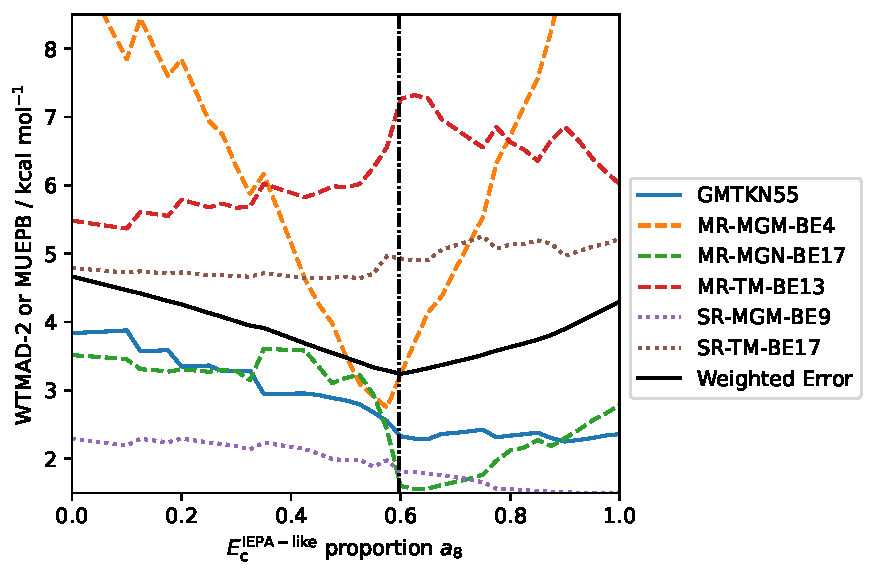
\includegraphics[width=0.6\textwidth]{assets/plot-seq-cr-proportion.pdf}
  \caption[XYG6+1/cr 在限制参数 $E_\textmt{c}^\textmt{EP}$ 占比系数下的参数优化误差表现]{XYG6+1/cr 在限制参数 $a_8$ 下对加权误差的拟合后数据集误差表现。}
  \label{fig.2.plot-seq-cr-proportion}
\end{figure}

首先考虑 EP 型相关能的引入。这里以 XYG6+1/cr 模型为例。图 \ref{fig.2.plot-seq-cr-proportion} 展示的是限制 $E_\textmt{c}^\textmt{MP2/cr}$ 在 $E_\textmt{c}^\textmt{PT}$ 效应中的占比数 $a_8$ 时,各数据子集误差随 $a_8$ 取值的变化情况。特别地,当取 $a_8 = 0$ (图像最右侧) 时,该模型化归为 XYG6 模型;当取 $a_8 = 1$ (图像最左侧) 时,该模型的微扰相关能完全是 MP2/cr;点划线表示加权误差取到最小时参数 $a_8$ 的数值,即 \ref{sec.2.xyg6-1-model-benchmark} 小节中所定义的 XYG6+1/cr 近似泛函。

受参数 $a_8$ 影响最大的数据集是 MR-MGM-BE4 (多参考主族金属键解离能);若不引入 ($a_8 = 0$) 或完全引入 ($a_8 = 1$) $E_\textmt{c}^\textmt{MP2/cr}$ 相关能,其 MUEPB 误差都将超过 8 \si{kcal.mol^{-1}}。事实上,从附录的表 \ref{tab.2.supp.MR-MGM-BE4} 中可以看到,XYG$n$ ($n=3,6,7$) 在 MR-MGM-BE4 测评中,阴离子 \ce{KO-} 与 \ce{LiO-} 的误差很大;其误差分别在 40 \si{kcal.mol^{-1}} 与 20 \si{kcal.mol^{-1}} 左右。这两个体系具有 1 eV 的小 HOMO/LUMO gap,因此可以预期到仅使用 MP2 相关能的 XYG$n$ ($n=3,6,7$) 在这类体系上表现较差。当 $a_8 \simeq 0.6$ 时,MP2/cr 的引入有效地缓解了这两个离子的误差到小于 10 \si{kcal.mol^{-1}},从而 MR-MGM-BE4 子集的 MUEPB 整体误差降至 3 \si{kcal.mol^{-1}} 左右。

对于其它数据集,一般来说,参数 $a_8$ 越大,越有利于 GMTKN55 数据集与 SR-MGM-BE9 子集的误差下降,尽管下降幅度较小;$a_8$ 对于 SR-TM-BE17 数据集的影响不大。需要指出的是,对于 $a_8 \simeq 0.6$ 的情形 (如表 \ref{tab.2.supp.SR-TM-BE17} 所示),SR-TM-BE17 数据集的 \ce{Zr2} 体系 HOMO/LUMO gap 是较小的 1.34 eV,处于 EP 型相关能可以对 MP2 相关能产生有效矫正的范围;在引入 EP 型相关能后计算误差相对于 XYG$n$ ($n=3,6,7$) 下降约 20 \si{kcal.mol^{-1}}。但同时因为其它计算体系的误差有小幅上升,因此 SR-MGM-BE9 子集的整体误差没有下降太多。

值得注意的是 MR-TM-BE13 与 MR-MGN-BE17 的表现在 XYG6+1/cr 模型下 $a_8 = 0.6$ 附近有较大的跳变;这个跳变的影响因素比较可能是间接地因参数优化过程中 $c_\textmt{x} = a_1$ 即严格交换能的占比跳变较大有关,如图 \ref{fig.2.plot-seq-cr-against-cx} 所示。可以发现,MR-TM-BE13 数据集的 MUEPB 误差通常随严格交换系数 $c_\textmt{x}$ 的增大而增大;相反地,MR-MGN-BE17 的 MUEPB 误差则随 $c_\textmt{x}$ 的增大而减小。因此,该误差跳变不能简单地归因于 MP2/cr 的引入本身。关于严格交换能占比参数 $c_\textmt{x}$ 对各数据集的影响,将在后一小节 \ref{sec.2.proportion-exchange} 中阐述。

\begin{figure}[h]
  \centering
  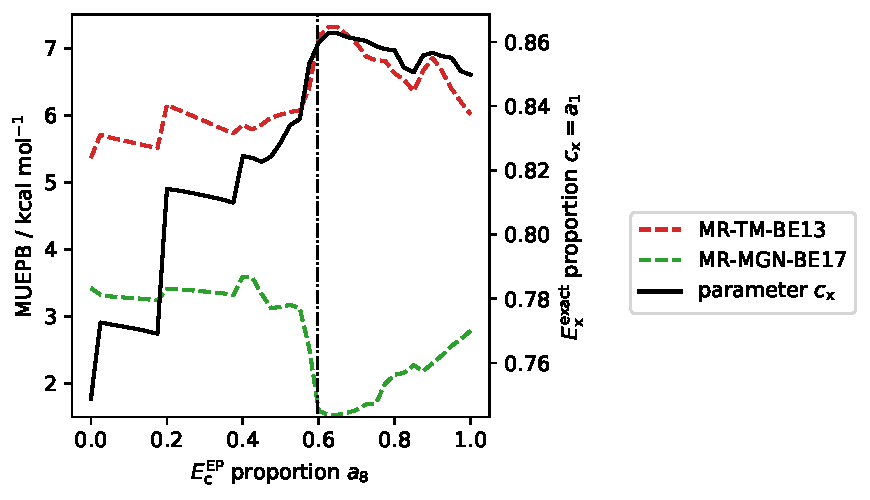
\includegraphics[width=0.6\textwidth]{assets/plot-seq-cr-against-cx.pdf}
  \caption[XYG6+1/cr 在限制参数 $E_\textmt{c}^\textmt{EP}$ 占比系数下误差与 $E_\textmt{x}^\textmt{exact}$ 系数表现]{XYG6+1/cr 在限制参数 $a_8$ 下对加权误差的拟合后 MR-TM-BE13、MR-MGN-BE17 数据集的 MUEPB 误差表现、以及参数 $c_\textmt{x} = a_1$ 在给定参数 $a_8$ 下的变化情况。}
  \label{fig.2.plot-seq-cr-against-cx}
\end{figure}

最后,我们考察引入 EP 型相关能后表现较差的体系。以 XYG6+1/cr 近似泛函为例,MR-TM-BE13 子集 (表 \ref{tab.2.supp.MR-TM-BE13}) 中的 \ce{TiCl}、\ce{NiCH2+}、\ce{VO} 以及 SR-TM-BE17 子集 (表 \ref{tab.2.supp.SR-TM-BE17}) 中的 \ce{CoH}、\ce{FeH}、\ce{FeCl},这些体系平均每个键的解离误差大于 10 \si{kcal.mol^{-1}}。由于这些体系的 HOMO/LUMO gap 均大于 1.5 eV,因此 MP2/cr 相关能与 MP2 相关能表现上会比较接近,从而难以通过仅引入 MP2/cr 相关能解决这类体系的计算误差。

\subsection{参数优化讨论:严格交换能占比}
\label{sec.2.proportion-exchange}

其次考察严格交换能的占比对数据集测评的影响。图 \ref{fig.2.plot-seq} 展示的是限制严格相关能 $E_\textmt{x}^\textmt{exact}$ 在总交换能中的占比数 $c_\textmt{x} = a_1$ 时,各数据子集误差随 $c_\textmt{x}$ 取值的变化情况。

首先,从上一小节 \ref{sec.2.proportion-iepa-like} 的讨论中,我们已经注意到 EP 型相关能的引入对 MR-MGM-BE4 子集的 MUEPB 测评表现、特别是 \ce{KO-} 与 \ce{LiO-} 离子的解离能有很大的提升;在图 \ref{fig.2.plot-seq} 中,可以清晰地看到在 $c_\textmt{x} > 0.5$ 时,XYG6+1 参数模型在 MR-MGM-BE4 的测评结果上明显优于没有引入 EP 型相关能的 XYG$n$ ($n=6,7$)。同时,对于 XYG6+1/cr 模型,其 GMTKN55、MR-MGN-BE17 与 MR-TM-BE13 在 $c_\textmt{x} > 0.5$ 时的误差相较于 XYG$n$ ($n=6,7$) 有一定提升,SR-MGM-BE9 与 SR-TM-BE17 的误差与 XYG$n$ ($n=6,7$) 接近;考虑到一般的双杂化泛函近似都选用 $c_\textmt{x} > 0.5$,因此图 \ref{fig.2.plot-seq} 的结果进一步验证了引入 EP、特别是 MP2/cr 相关能,对整体误差表现确实有所提升。

但对于其它数据集而言,不论选取哪一种模型,总体上
\begin{itemize}[nosep]
  \item $c_\textmt{x}$ 愈接近 0.9,GMTKN55 数据集的 WTMAD-2 误差愈小;
  \item $c_\textmt{x}$ 愈接近 0.5,MR-TM-BE13 子集的 MUEPB 误差愈小;
  \item SR-TM-BE17 子集的误差比较平稳,在 $c_\textmt{x}$ 取 0.7 时通常较小。
\end{itemize}
考虑到 GMTKN55 数据集在拟合过程中的权重较大、MR-TM-BE13 与 MR-MGM-BE4 子集的误差本身较大,且这三个数据集误差对 $c_\textmt{x}$ 的变化比较敏感,因此对泛函模型进行参数优化时,$c_\textmt{x}$ 取值事实上平衡这三个数据集的误差。由于 EP 型相关能的引入大幅降低了 MR-MGM-BE4 的误差、并一定程度地降低了 MR-TM-BE13 的误差以及其对 $c_\textmt{x}$ 取值的敏感程度,因此 XYG6+1 模型所优化得到的参数中 $c_\textmt{x}$ 取值比较接近 GMTKN55 数据集下表现良好的范围即 $c_\textmt{x} \simeq 0.9$。而对于 XYG$n$ ($n=6,7$) 模型而言,降低参数 $c_\textmt{x}$ 可以在牺牲一定的 GMTKN55 误差时显著降低 MR-TM-BE13 与 MR-MGM-BE4 的误差,因此参数这类模型倾向于优化 $c_\textmt{x}$ 到大约 0.7 左右。

\begin{figure}[h]
  \centering
  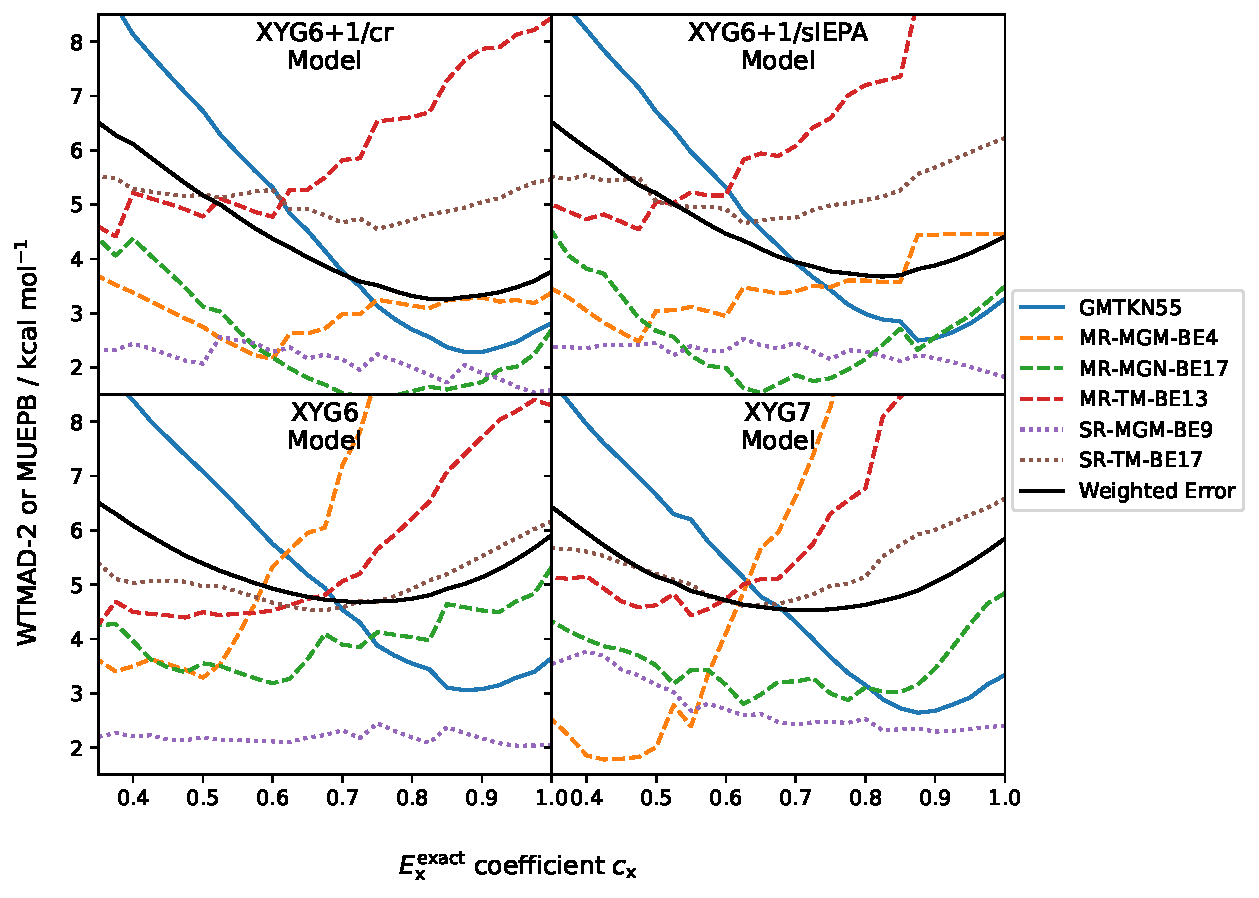
\includegraphics[width=0.9\textwidth]{assets/plot-seq.pdf}
  \caption[诸参数模型在限制 $E_\textmt{x}^\textmt{exact}$ 系数下参数优化后误差]{诸参数模型在限制参数 $c_\textmt{x} = a_1$ 下对加权误差的拟合后数据集的误差表现。}
  \label{fig.2.plot-seq}
\end{figure}

Yu 等\cite{Yu-Truhlar.CS.2016} 认为,Hartree-Fock 交换能通常可以提升碳水化合物、弱相互作用、反应能垒等问题上有较好的表现 (这些也是 GMTKN55 数据集着重关心的问题),但会破坏多参考体系问题的表现。尽管 Yu 等的主张针对杂化泛函,但图 \ref{fig.2.plot-seq} 表明在 $c_\textmt{x} > 0.5$ 的情形下表明基于 B3LYP 轨道的双杂化泛函也有相同的结论。

XYG6+1 模型尽管对以 \ce{KO-}、\ce{LiO-}、\ce{Zr2} 为代表的 HOMO/LUMO gap 较小的计算问题有更好的处理,但需要指出的是,尽管引入了 EP 型相关能的 XYG6+1 模型一定程度上减少了 MR-TM-BE13 的误差,但减小幅度远小于降低 $c_\textmt{x}$ 所带来的收益;类如 \ce{TiCl}、\ce{NiCH2+}、\ce{VO}、\ce{CoH}、\ce{FeH}、\ce{FeCl} 等困难的计算问题,一定程度地降低 $c_\textmt{x}$ 尽管能有更好的计算表现,但同时会推高 GMTKN55 为代表的主族化学问题的误差。因此需要承认,为要更好地解决这两类问题,仅使用引入 EP 型相关能的 XYG6+1 框架仍然是不够的。

\subsection{参数优化讨论:数据集的影响}
\label{sec.2.propotion-dataset}

简单讨论引入 Minnesota 2015 数据集与否,对参数优化结果的影响。图 \ref{fig.2.plot-seq-xyg7} 展示了 XYG6+1/cr 模型下,仅对 GMTKN55 数据集参数优化、与额外引入 Minnesota 2015 五个数据子集参数优化的误差比较。可以看到,引入额外的数据集、并重新定义误差量标,确实会使得部分数据子集的误差表现有明显的变化。引入 Minnesota 2015 数据集进行优化后,在所有图中展示的 $c_\textmt{x}$ 区域内对 GMTKN55 的 WTMAD-2 误差量标有大约 0.5 \si{kcal.mol^{-1}} 的增加。因此,GMTKN55 的误差总体变化不大;由于我们在构造加权误差时对 GMTKN55 的 WTMAD-2 施加权重为很大的 48\%,因此 GMTKN55 的误差变化较小是可以预期的。

当 Minnesota 2015 五个数据子集纳入拟合集时,尽管每个子集分到的权重不超过 12\%,但除 SR-MGM-BE9 外的数据子集误差显著下降;SR-MGM-BE9 的误差在 $c_\textmt{x} > 0.5$ 的范围内也可以控制在 3 \si{kcal.mol^{-1}} 以内。这意味着,从积极的角度来看,即使参数拟合没有严重地偏向于每一个参与加权误差计算的 Minnesota 2015 数据子集,XYG6+1/cr 模型也能在不严重影响 GMTKN55 误差的前提下,较好地改善这些子集的表现,从而在更广泛的化学问题上有优异的表现。但从消极的角度看,也意味着在当前的加权误差标准下,这些 Minnesota 2015 子集的误差对 XYG6+1/cr 模型的参数并不是非常稳健;若对加权误差的表达式作较大程度的改变、或引入其它数据集参与参数拟合,这些子集的误差有很大可能会被较大程度地改变。

同时需要注意到,若没有引入 Minnesota 2015 数据子集、而仅以 GMTKN55 数据集进行拟合时,XYG6+1/cr 模型对这五个数据子集 (如图 \ref{fig.2.plot-seq-xyg7} 左侧所示) 的预测表现不能称为良好。若以此现象外推,则不能期望 \ref{sec.2.xyg6-1-model-benchmark} 小节所提出的 XYG6+1/cr 近似泛函可以以与 GMTKN55 和 Minnesota 2015 五个数据子集相同的精度解决被拟合的数据集以外的化学问题。这部分的讨论对除 MP2/cr 以外的其它掺杂 EP 型相关能的 XYG6+1 参数模型泛函同样适用。

\begin{figure}[h]
  \centering
  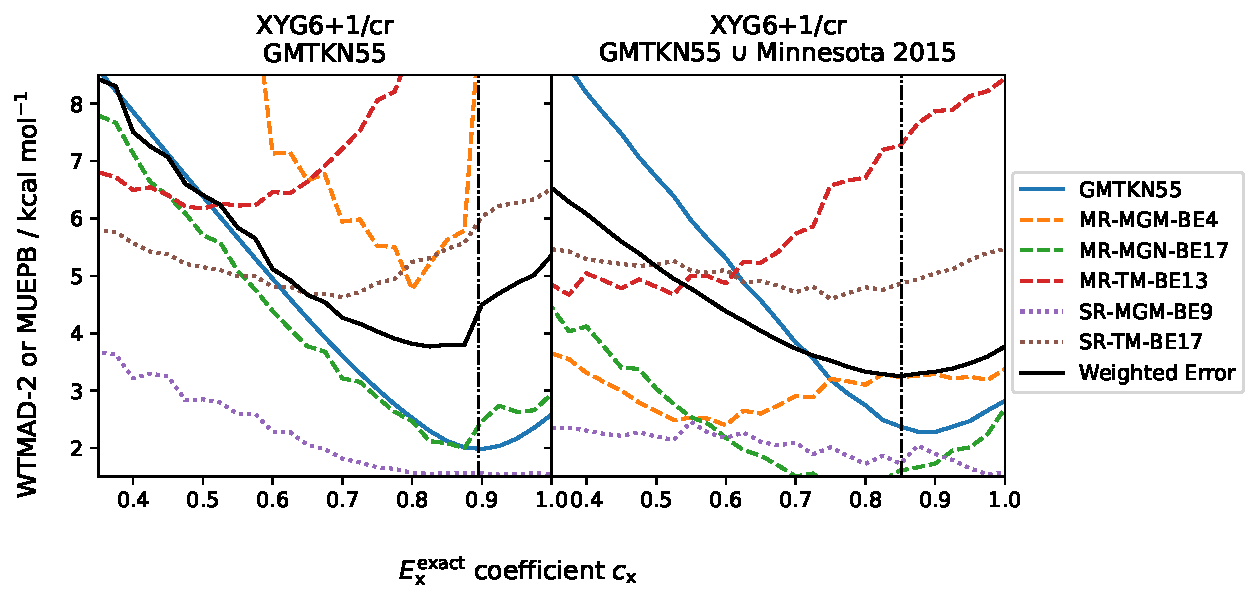
\includegraphics[width=0.9\textwidth]{assets/plot-seq-cr.pdf}
  \caption[XYG6+1/cr 模型在限制 $E_\textmt{x}^\textmt{exact}$ 系数下不同参数优化策略测评误差]{XYG6+1/cr 模型在限制参数 $c_\textmt{x} = a_1$ 下对数据集拟合后数据集的误差表现。左图针对 GMTKN55 的 WTMAD-2 误差量标优化,右图针对 GMTKN55 与 Minnesota 2015 五个子集的加权误差量标优化。点划线表示在对应误差量标下 $c_\textmt{x}$ 的最佳取值。}
  \label{fig.2.plot-seq-xyg7}
\end{figure}

\subsection{XYG6+1 模型泛函在分子解离曲线问题的表现}

在本节最后,将简短地考察 XYG6+1 模型泛函的在部分分子解离曲线问题的表现。

作为三键体系,\ce{N2} 氮气解离问题是最有挑战性的分子解离势能面问题之一。在图 \ref{fig.2.curve-N2} 中可以看到,在解离曲线 1.0--2.0 \AA 的范围内,XYG6+1/cr 方法与 DMC 方法之间的误差普遍在 30 \si{kcal.mol^{-1}} 以内;而 XYG6+1/IEPA 方法与 CCSD(T)、DMC 方法的结果在 1.0--2.0 \AA 非常接近。XYG6+1/sIEPA 尽管存在较大误差,但相较于 MP2、MP2/cr-III、XYG$n$ ($n=3,7$) 等方法,在键长超过 1.4 \AA 时严重下行的趋势上有所改善。

但需要指出,在图中所测评的基于单参考态的近似方法中,几乎没有可以正确预言超过 2.0 \AA 后解离的趋势。CCSD 方法尽管在解离后段趋于准确值 (两个氮原子的能量和),但由于在 1.0--2.0 \AA 区间高估了解离趋势,因此产生了非物理的凸包。CCSD(T) 与 XYG6+1/cr 方法尽管在 1.0--2.0 \AA 的范围内表现良好,但在 2.0 \AA 以后的区域有明显下行趋势。XYG6+1/sIEPA 与 XYG6+1/IEPA 方法则在 2.0 \AA 以后的区域有明显的上行趋势;这是因为尽管 sIEPA 与 IEPA 相关能的趋势是下行,但 MP2 相关能相比于 sIEPA 与 IEPA 相关能下行趋势要明显地多;而 XYG6+1/sIEPA 与 XYG6+1/IEPA 的 MP2 在总微扰型相关能中的占比分别约为 -0.42\% 和 -0.11\%,由于 MP2 相关能负系数的原因,XYG6+1/sIEPA 与 XYG6+1/IEPA 显现出了与 MP2 相反的上升趋势。由于 XYG6+1/sIEPA 中 MP2 相关能的负系数占比更大,因此 XYG6+1/sIEPA 比 XYG6+1/IEPA 更早、更明显地在势能面上显现出错误的上升趋势。

\begin{figure}[h]
  \centering
  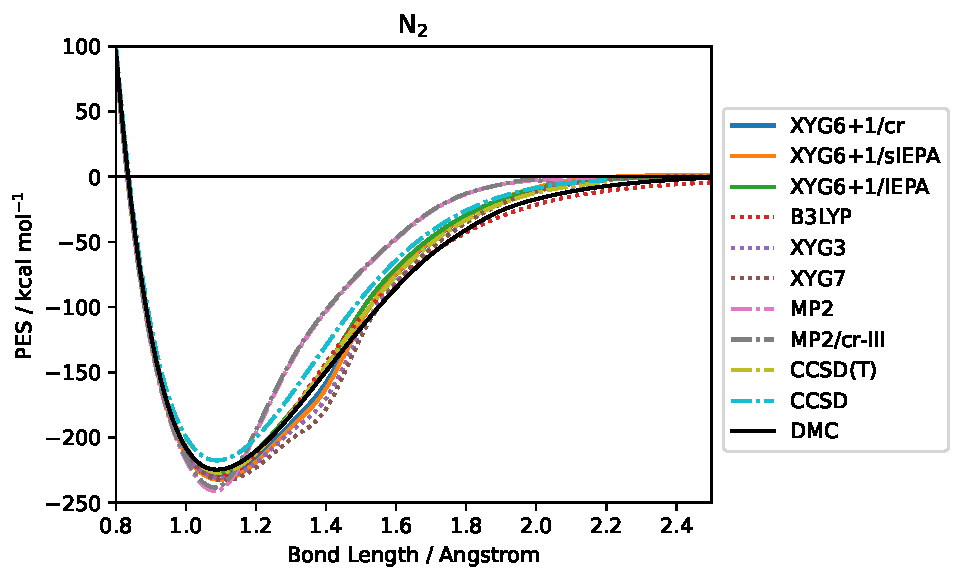
\includegraphics[width=0.7\textwidth]{assets/curve-N2.pdf}
  \caption[\ce{N2} 解离曲线表现]{各方法在 \ce{N2} 解离曲线的表现。}
  \label{fig.2.curve-N2}
\end{figure}

随后考虑 \ce{F2} 解离曲线。在图 \ref{fig.2.curve-F2} 中,仍然没有方法能完全正确地预言合理的解离趋势。尽管 CCSD(T) 的 \ce{F2} 解离曲线在 1.2 \AA 后始终是倾向于成键的 (势能面的能量在 0 \si{kcal.mol^{-1}} 以下),但在 2.2 \AA 以后显现出不正确的下行趋势。XYG6+1/cr、XYG6+1/sIEPA 与 XYG$n$ (n=3,7) 在 1.2--1.6 \AA 的成键区域中,能量与 CCSD(T) 非常接近。但在 2.0 \AA 后的区域中,XYG$n$ ($n=3,7$) 有着比 CCSD(T) 更加严重的下行。相反地,诸 XYG6+1 近似泛函与 CCSD、B3LYP、MP2/cr-III 等方法则在成键区域以后严重高估势能面;这些方法在 1.6--2.0 \AA 的区域中有比较接近的数值。

\begin{figure}[h]
  \centering
  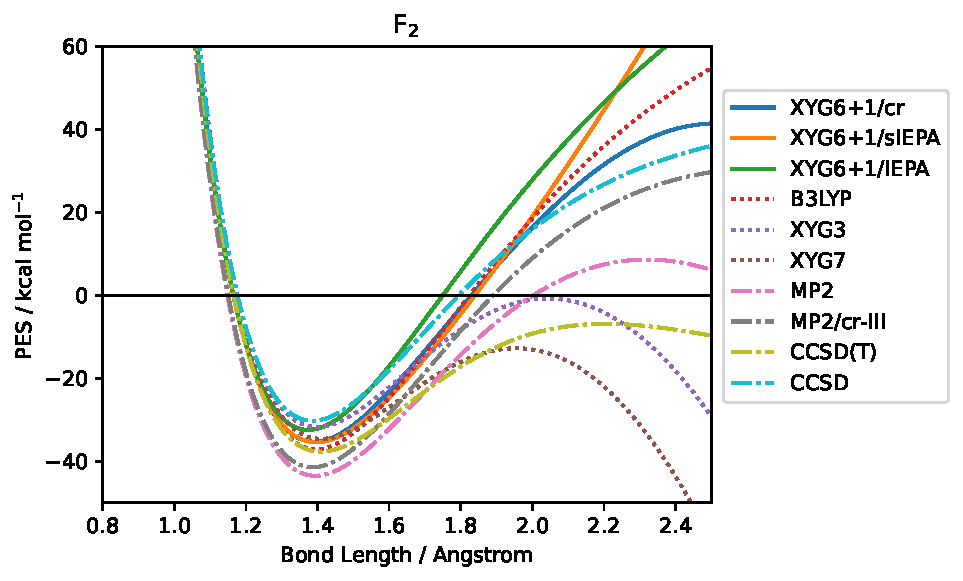
\includegraphics[width=0.7\textwidth]{assets/curve-F2.pdf}
  \caption[\ce{F2} 解离曲线表现]{各方法在 \ce{F2} 解离曲线的表现。}
  \label{fig.2.curve-F2}
\end{figure}

\ce{H2O} 与 \ce{F2} 体系同样是单键解离问题。从图 \ref{fig.2.curve-H2O} 与图 \ref{fig.2.curve-H2O-part} 中可以看出,相比于 \ce{F2},各方法在 \ce{H2O} 体系上的表现明显普遍较好,但仍然存在一些问题。CCSD(T)、XYG3 方法在 2.0 \AA 以前与 DMC 的结果非常接近,但 2.0 \AA 以后显现出下降的趋势。XYG7 在解离曲线后期普遍低估能量。除 CCSD(T)、XYG$n$ ($n=3, 7$) 外的方法则对解离曲线有一定程度的高估;其中 MP2 与 XYG6+1/sIEPA 方法在 1.4--1.8 \AA 与作为参考值的 DMC 结果非常接近、其它方法则在这一段解离曲线上也稍有误差。

\begin{figure}[h]
  \centering
  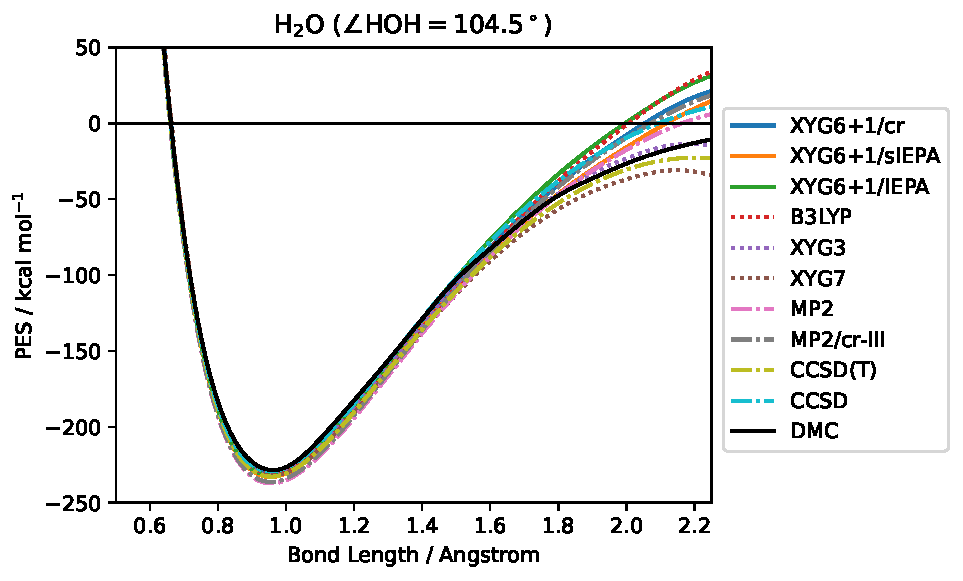
\includegraphics[width=0.7\textwidth]{assets/curve-H2O.pdf}
  \caption[\ce{H2O} 解离曲线表现]{各方法在 \ce{H2O} 解离曲线的表现。}
  \label{fig.2.curve-H2O}
\end{figure}

\begin{figure}[h]
  \centering
  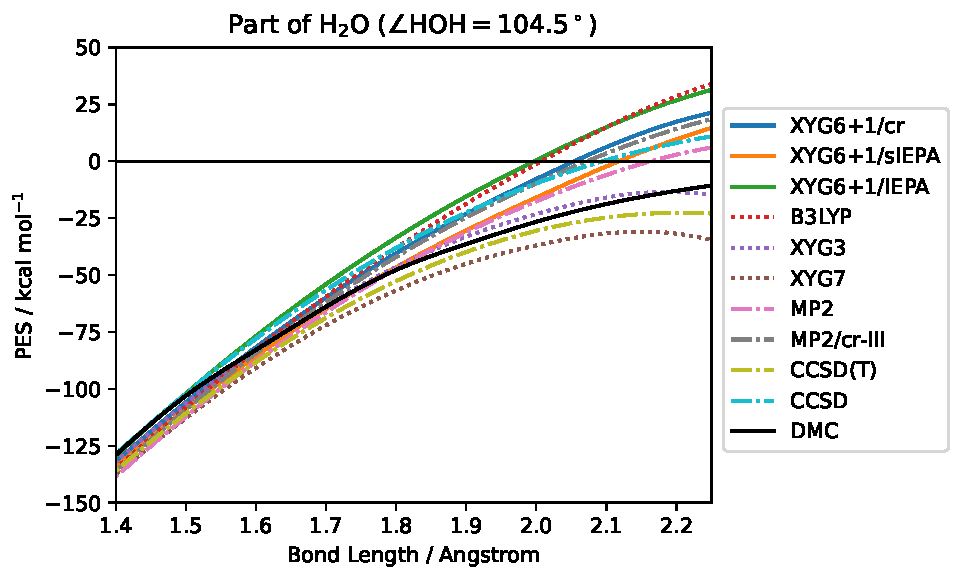
\includegraphics[width=0.7\textwidth]{assets/curve-H2O-part.pdf}
  \caption[\ce{H2O} 解离曲线 1.4--2.25 \AA 段表现]{各方法在 \ce{H2O} 解离曲线 1.4--2.25 \AA 段的表现。}
  \label{fig.2.curve-H2O-part}
\end{figure}

作为一种不太常规的单键解离问题,图 \ref{fig.2.curve-H6} 所示的环状 \ce{H6} 解离曲线也有一定挑战性。对于 CCSD 与 CCSD(T) 方法,它们在 1.8 \AA 以前的表现骄傲好,但在 2.0 \AA 以后能量明显地出现了不符合物理直觉的下降。MP2 与 MP2/cr-III 方法则不管是在 0.75--1.25 \AA 的成键区域、还是以后的解离区域,相比于参考值 DMC 都有一定程度的高估。B3LYP 在成键区域低估、但在解离区域则明显高估势能面上的能量。对于经测评的 xDH 型泛函,他们都在成键区域有良好的表现,但在解离区域产生明显的高估。

\begin{figure}[h]
  \centering
  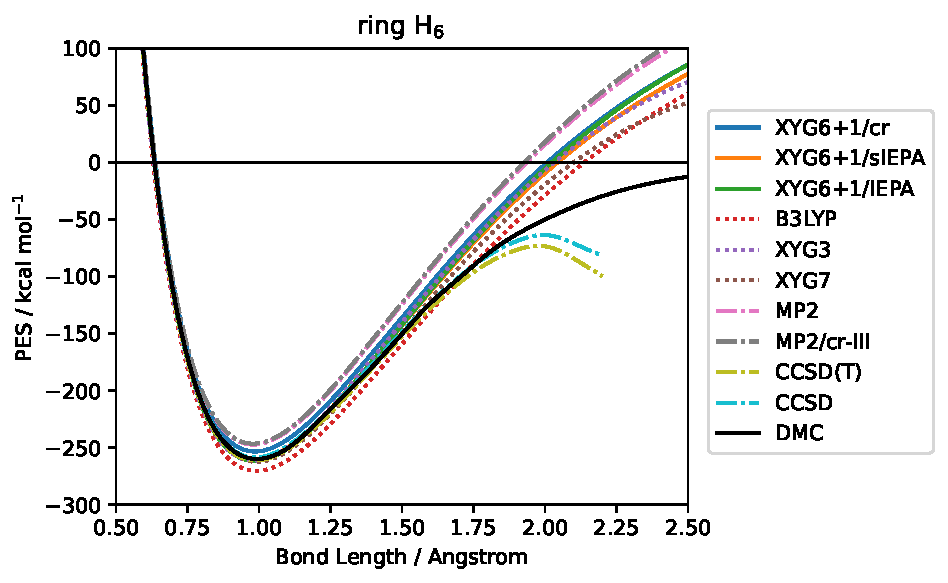
\includegraphics[width=0.7\textwidth]{assets/curve-H6.pdf}
  \caption[\ce{H6} 解离曲线表现]{各方法在 \ce{H6} 解离曲线的表现。}
  \label{fig.2.curve-H6}
\end{figure}

从上述的讨论中,我们看到大多数情形下,xDH 型泛函和 CCSD、CCSD(T) 方法在成键区域的势能面与参考值非常接近。但即使是计算化学中普遍受到认可的高精度 CCSD 与 CCSD(T) 方法,在闭壳层的限制下,也难以给出定性上正确的解离曲线;而对于其它 post-HF 与密度泛函近似方法更是如此。引入 EP 类型相关能的诸 XYG6+1 模型可以在 \ce{N2} 问题上,相较于 XYG$n$ ($n=3,7$) 有很大程度的改善,成功地避免了解离过程中段过于严重的负误差;但正因为一般来说 EP 型相关能绝对值小于 MP2 相关能、并且 HOMO/LUMO gap 愈小 EP 型相关能与 MP2 相关能之间的差距愈大,因此绝大多数情况下诸多 XYG6+1 模型近似泛函的势能面比 XYG$n$ 模型要高。对于所有经测评的单键解离体系,相比于 DMC 参考值、或者解离极限的原子能量之和而言,XYG$n$ ($n=3,7$) 的势能面在解离区域已经有较大程度的高估;在这种情况下,正因为引入了 EP 型相关能,XYG6+1 模型实际上会更严重地高估势能面。因此,我们无法给出简单的结论,表明 XYG6+1 模型是否在解离曲线问题上,相比于 XYG$n$ ($n=3,7$) 是否有改善。

\section{本章小结}

在本章工作中,我们简单回顾了作为双杂化泛函理论基础的 G\"orling-Levy 微扰理论。该理论联系起 post-HF 方法与密度泛函近似。作为该微扰理论的近似,GLPT2 是诸多双杂化泛函的理论基础。GLPT2 一般由 MP2 相关能实现,而 MP2 相关能在 HOMO/LUMO gap 较小时存在明显的负误差。籍此,我们简单梳理了 IEPA 与 MP2/cr 的理论,并表明这些 EP 型相关能可以缓解 MP2 相关能在 HOMO/LUMO gap 较小情况下的误差。类似于 post-HF 框架之于 IEPA 的关系,我们对 G\"orling-Levy 微扰框架下引入 EP 型相关能的理论合理性作了说明。

为缓解基于 MP2 型相关能的双杂化泛函在以 \ce{N2} 解离、含过渡金属体系为代表的 HOMO/LUMO gap 较小体系上存在一定负误差的情况,同时保证在以主族反应势垒、键解离能、弱相互作用能为代表的、主流双杂化泛函表现较好的问题上保持较小的误差,我们尝试在 GMTKN55 数据集上有优异表现的 xDH@B3LYP 框架下引入 EP 型相关能以构造新的 XYG6+1 参数模型。在参数优化上,除了着重主族化学的 GMTKN55 外,我们引入部分含有多参考信息与过渡金属信息的 Minnesota 2015 子数据集,作参数优化得到新的泛函近似;它们依引入的相关能形式不同,称为 XYG6+1/cr、XYG6+1/IEPA 与 XYG6+1/sIEPA。

参数优化与测评结果表明,XYG6+1/cr 近似泛函在各个数据集上的表现有良好的平衡。对于 \ce{KO-}、\ce{LiO-}、\ce{Zr2} 等 HOMO/LUMO gap 小于 1.5 eV 的体系,键解离能的计算误差从 20--40 \si{kcal.mol^{-1}} 降到 10 \si{kcal.mol^{-1}} 以下,有效地降低了这类体系误差。同时,XYG6+1/cr 在 GMTKN55 数据集上的总体 WTMAD-2 误差为 2.36 \si{kcal.mol^{-1}},其表现相比于目前流行的 MP2 型相关能的双杂化泛函仍然良好;在我们所定义的 GMTKN55 和 Minnesota 2015 部分子数据集上的加权误差为 3.28 \si{kcal.mol^{-1}},是表现最优异的泛函。XYG6+1/cr 很好地平衡了主族化学问题与多参考特性或过渡金属问题的误差,基本达到了设计该泛函近似的初衷。XYG6+1/sIEPA 泛函也有类似的良好表现。

但需要承认,仅引入 EP 型相关能、并作关于 GMTKN55 和 Minnesota 2015 部分子数据集的优化得到的泛函,仍然存在着困难。
\begin{itemize}[nosep]
  \item 首先,HOMO/LUMO gap 小的体系一般具有多参考特性,但多参考特性的体系 HOMO/LUMO gap 不一定小;在诸如 \ce{TiCl}、\ce{NiCH2+}、\ce{VO} 为代表的多参考特性的体系上,XYG6+1 模型泛函表现较差。此外,诸如 \ce{CoH}、\ce{FeH}、\ce{FeCl} 等单参考特性含过渡金属体系的键解离也存在较大误差,而多参考特性的 MR-MGN-BE17 数据集的总的误差相当低,表明 XYG6+1 模型的误差来源与单参考或多参考的关联性不一定很强,而可能与过渡金属本身关联性稍大。
  \item 在分子解离曲线问题上,在闭壳层限制下,尽管 XYG6+1 参数模型在 \ce{N2} 体系上 2.0 \AA 以前的表现较好,但仍然无法避免解离到更远时定性不正确的趋势;而在以 \ce{F2}、\ce{H2O}、环状 \ce{H6} 为代表的单键解离问题上,不论是否引入 EP 型或 MP2 型相关能,都在解离区域存在较大的正误差。这意味着在密度泛函近似中,仅仅矫正 MP2 相关能在 HOMO/LUMO gap 较小时的误差表现,不足以漂亮地解决解离曲线的问题。
  \item 对参数优化过程的讨论,表明严格交换能 $E_\textmt{x}^\textmt{exact}$ 占比愈大对 GMTKN55 主族化学问题的误差愈小、但相应地 MR-TM-BE13 等含过渡金属或多参考特性体系的数据集误差愈大;这个现象并不因为在泛函中引入 EP 型相关能而有所改善。同时,对于 XYG6+1 参数模型优化得到的泛函,误差容易随参与拟合数据集的变化而波动,表明该参数模型下的泛函不是非常稳健。我们无法建议将 XYG6+1 参数模型下优化的泛函,应用在 GMTKN55 与 Minnesota 2015 五个子数据集的目标化学问题以外的体系计算上。
\end{itemize}

\clearpage

\section{附录:补充数据}

\begin{table}[ht]
\centering
\caption[MR-MGM-BE4 子集测评误差]{部分 xDH@B3LYP 模型与 XYG6+1 模型近似泛函在 MR-MGM-BE4 子集上误差。\\反应能与 MUEPB 单位 \si{kcal.mol^{-1}};HOMO/LUMO gap 单位 eV。}
\label{tab.2.supp.MR-MGM-BE4}
\widetabular{
  \begin{tabular}{ld{1.2}d{3.2}d{3.2}d{3.2}d{3.2}d{3.2}d{3.2}}
  \toprule
  \multicolumn{2}{c}{MR-MGM-BE4} & \multicolumn{3}{c}{xDH@B3LYP} & \multicolumn{3}{c}{XYG6+1\tnote{a}} \\
  \cmidrule(lr){1-2} \cmidrule(lr){3-5} \cmidrule(lr){6-8}
  体系 & \multicolumn{1}{c}{gap} & 
  \multicolumn{1}{c}{XYG3} & \multicolumn{1}{c}{XYG6} & \multicolumn{1}{c}{XYG7} &
  \multicolumn{1}{c}{MP2/cr} & \multicolumn{1}{c}{sIEPA} & \multicolumn{1}{c}{IEPA} \\
  \midrule
  \ce{CaO } & 2.54 & 7.01  & 8.03  & 1.50  & 1.41      & 0.18         & 0.68        \\
  \ce{KO- } & 1.03 & 38.03 & 56.57 & 46.24 & 0.00      & 0.00         & 0.00        \\
  \ce{LiO-} & 1.03 & 19.40 & 25.28 & 20.65 & 5.80      & 9.54         & 3.99        \\
  \ce{MgS } & 1.75 & -3.27 & -1.52 & -2.83 & -5.75     & -4.77        & -5.81       \\
  \midrule
  MUEPB     &      & 16.93 & 22.85 & 17.81 & 3.24      & 3.62         & 2.62        \\
  \bottomrule
  \end{tabular}
}{
  \item[a] 为方便排版,表头第二行指代的是 XYG6+1 模型泛函所使用的 EP 型相关能 $E_\textmt{c}^\textmt{EP}$ 的具体类型;即 MP2/cr 指代 XYG6+1/cr、sIEPA 指代 XYG6+1/sIEPA、IEPA 指代 XYG6+1/IEPA。后续表格类同。
}
\end{table}

\begin{table}[ht]
\centering
\caption[MR-MGN-BE17 子集测评误差]{部分 xDH@B3LYP 模型与 XYG6+1 模型近似泛函在 MR-MGN-BE17 子集上误差。\\反应能与 MUEPB 单位 \si{kcal.mol^{-1}};HOMO/LUMO gap 单位 eV。}
\label{tab.2.supp.MR-MGN-BE17}
\widetabular{
  \begin{tabular}{ld{2.2}d{3.2}d{3.2}d{3.2}d{3.2}d{3.2}d{3.2}}
  \toprule
  \multicolumn{2}{c}{MR-MGN-BE17} & \multicolumn{3}{c}{xDH@B3LYP} & \multicolumn{3}{c}{XYG6+1} \\
  \cmidrule(lr){1-2} \cmidrule(lr){3-5} \cmidrule(lr){6-8}
  体系\tnote{a} & \multicolumn{1}{c}{gap\tnote{b}} & 
  \multicolumn{1}{c}{XYG3} & \multicolumn{1}{c}{XYG6} & \multicolumn{1}{c}{XYG7} &
  \multicolumn{1}{c}{MP2/cr} & \multicolumn{1}{c}{sIEPA} & \multicolumn{1}{c}{IEPA} \\
  \midrule
  \ce{NF3 }          &  10.08 & -2.57 & -0.70 & -1.54 & -0.60     & -0.89        & -1.13       \\
  \ce{CO2 }          &  9.87  & -0.40 & 1.84  & -0.25 & 0.61      & 0.42         & -0.12       \\
  \ce{SiO }          &  6.34  & 1.65  & 3.88  & 1.26  & -0.22     & 0.00         & -2.69       \\
  \ce{SO2 }          &  5.69  & -1.34 & 1.50  & -0.71 & -0.84     & -0.99        & -2.35       \\
  \ce{CO2 }          &  9.41  & -1.06 & 1.84  & -0.11 & -0.25     & 0.10         & -2.29       \\
  \ce{SO2 }          &  3.69  & 0.29  & 0.41  & -0.87 & -1.46     & -3.63        & -1.81       \\
  \ce{ClO }          &  2.78  & -1.94 & -0.71 & -1.48 & -1.95     & -3.02        & -2.43       \\
  \ce{F2  }          &  7.23  & -6.91 & -2.23 & -4.17 & -3.35     & -3.28        & -6.35       \\
  \ce{N2  }          &  10.99 & 1.17  & 2.60  & 2.31  & -1.35     & 1.97         & -3.23       \\
  \ce{O2  }          &  5.28  & -1.09 & -1.29 & -1.67 & -2.65     & -7.06        & -3.60       \\
  \ce{NO  }          &  3.01  & -0.43 & 1.33  & 0.77  & -1.27     & -0.43        & -3.02       \\
  \ce{CN  }          &  3.58  & 2.82  & 5.52  & 3.05  & -0.28     & 0.89         & -3.54       \\
  \ce{B2  }          &  2.17  & -1.12 & 2.16  & -0.67 & -5.74     & -9.10        & -7.72       \\
  \ce{O3  }\tnote{c} &  4.12  & 0.30  & 13.49 & 8.35  & 0.06      & 3.59         & -7.78       \\
  \ce{C2  }          &  1.80  & 4.19  & 17.97 & 10.48 & -5.59     & -2.42        & -15.25      \\
  \ce{S4  }\tnote{d} &  2.28  & 1.56  & 9.44  & 6.47  & -1.59     & 2.84         & -2.51       \\
  \ce{Cl2O}\tnote{e} &  4.31  & -1.98 & 0.60  & -0.61 & -0.29     & -0.45        & -1.64       \\
  \midrule
  MUEPB              &        & 1.81  & 3.97  & 2.63  & 1.65      & 2.42         & 3.97        \\
  \bottomrule
  \end{tabular}
}{
  \item[a] 对于未标明化学反应式的体系,其对应的反应是原子化反应。后续表格类同。
  \item[b] 对于开壳层体系,HOMO/LUMO gap 是通过 $\alpha, \beta$ 两种自旋的 HOMO 最大值与 LUMO 最小值的差减计算得到。后续表格类同。
  \item[c] \ce{O3 -> O2 + O}
  \item[d] \ce{S4 -> 2 S2}
  \item[e] \ce{Cl2O -> Cl2 + O}
}
\end{table}

\begin{table}[ht]
\centering
\caption[MR-TM-BE13 子集测评误差]{部分 xDH@B3LYP 模型与 XYG6+1 模型近似泛函在 MR-TM-BE13 子集上误差。\\反应能与 MUEPB 单位 \si{kcal.mol^{-1}};HOMO/LUMO gap 单位 eV。}
\label{tab.2.supp.MR-TM-BE13}
\widetabular{
  \begin{tabular}{ld{1.2}d{3.2}d{3.2}d{3.2}d{3.2}d{3.2}d{3.2}}
  \toprule
  \multicolumn{2}{c}{MR-TM-BE13} & \multicolumn{3}{c}{xDH@B3LYP} & \multicolumn{3}{c}{XYG6+1} \\
  \cmidrule(lr){1-2} \cmidrule(lr){3-5} \cmidrule(lr){6-8}
  体系 & \multicolumn{1}{c}{gap} & 
  \multicolumn{1}{c}{XYG3} & \multicolumn{1}{c}{XYG6} & \multicolumn{1}{c}{XYG7} &
  \multicolumn{1}{c}{MP2/cr} & \multicolumn{1}{c}{sIEPA} & \multicolumn{1}{c}{IEPA} \\
  \midrule
  \ce{TiCl    }          & 5.72 & -10.78 & -13.28 & -15.27 & -12.64    & -18.46       & -10.47      \\
  \ce{VF5     }          & 5.94 & 5.37   & 9.00   & 6.49   & 5.15      & 3.76         & 0.96        \\
  \ce{CrCl    }          & 2.93 & 3.09   & 3.13   & 3.18   & 1.10      & 2.35         & 0.69        \\
  \ce{CrOF    }          & 1.68 & -5.09  & 0.04   & -3.31  & -6.61     & -4.28        & -11.81      \\
  \ce{(FeBr2)2}          & 2.73 & 8.23   & 9.72   & 10.04  & 8.49      & 8.91         & 8.22        \\
  \ce{Co(CO)4H}          & 5.89 & 20.39  & 27.69  & 23.02  & 13.45     & 13.98        & 8.34        \\
  \ce{NiCH2+  }\tnote{a} & 3.90 & 18.44  & 20.94  & 18.52  & 12.16     & 8.34         & 8.73        \\
  \ce{FeCO5   }\tnote{b} & 4.96 & 24.37  & 29.99  & 26.32  & 12.90     & 15.84        & 11.56       \\
  \ce{VS      }          & 2.90 & 14.57  & 17.19  & 15.79  & 3.69      & 3.25         & -0.99       \\
  \ce{CuCl    }          & 3.99 & 1.28   & 3.15   & 2.59   & 1.21      & 1.81         & 0.75        \\
  \ce{CuH     }          & 4.23 & 2.29   & 2.91   & 3.57   & 0.97      & 2.20         & 0.33        \\
  \ce{NiCl    }          & 3.14 & 4.75   & 6.76   & 5.81   & 4.17      & 4.08         & 2.89        \\
  \ce{VO      }          & 2.55 & 20.04  & 27.78  & 23.64  & 13.58     & 13.49        & 3.22        \\
  \midrule
  MUEPB                  &      & 10.67  & 13.20  & 12.12  & 7.40      & 7.75         & 5.30        \\
  \bottomrule
  \end{tabular}
}{
  \item[a] \ce{NiCH2+ -> Ni+ + CH2}
  \item[b] \ce{FeCO5 -> Fe + 5CO}
}
\end{table}

\begin{table}[ht]
\centering
\caption[SR-MGM-BE9 子集测评误差]{部分 xDH@B3LYP 模型与 XYG6+1 模型近似泛函在 SR-MGM-BE9 子集上误差。\\反应能与 MUEPB 单位 \si{kcal.mol^{-1}};HOMO/LUMO gap 单位 eV。}
\label{tab.2.supp.SR-MGM-BE9}
\widetabular{
  \begin{tabular}{ld{1.2}d{3.2}d{3.2}d{3.2}d{3.2}d{3.2}d{3.2}}
  \toprule
  \multicolumn{2}{c}{SR-MGM-BE9} & \multicolumn{3}{c}{xDH@B3LYP} & \multicolumn{3}{c}{XYG6+1} \\
  \cmidrule(lr){1-2} \cmidrule(lr){3-5} \cmidrule(lr){6-8}
  体系 & \multicolumn{1}{c}{gap} & 
                 \multicolumn{1}{c}{XYG3} & \multicolumn{1}{c}{XYG6} & \multicolumn{1}{c}{XYG7} &
                 \multicolumn{1}{c}{MP2/cr} & \multicolumn{1}{c}{sIEPA} & \multicolumn{1}{c}{IEPA} \\
  \midrule
  \ce{AlCl3}          & 7.35 & 0.02  & 0.72  & -0.07 & -0.11     & 0.29         & 0.55        \\
  \ce{AlF3 }          & 9.43 & -1.23 & -0.30 & -3.03 & -0.74     & -1.39        & -1.18       \\
  \ce{KOH  }\tnote{a} & 3.72 & -1.73 & -0.79 & -3.14 & -2.71     & -2.55        & -3.59       \\
  \ce{NaO  }          & 3.09 & -2.18 & -2.62 & -4.22 & -4.25     & -3.79        & -4.47       \\
  \ce{LiO  }          & 3.41 & 1.83  & 0.52  & -0.92 & -0.72     & -0.12        & -0.03       \\
  \ce{LiCl }          & 5.31 & -0.87 & -1.58 & -2.43 & -2.99     & -2.17        & -2.00       \\
  \ce{AlCl3}          & 5.01 & -0.05 & 0.39  & -0.26 & -0.81     & -0.39        & -0.32       \\
  \ce{ZnSe }          & 1.64 & 6.16  & 7.86  & 7.89  & 4.51      & 5.43         & 4.55        \\
  \ce{ZnCl }          & 2.34 & 0.25  & 1.22  & 0.97  & 0.93      & 0.75         & 1.54        \\
  \midrule
  MUEPB              &      & 1.59  & 1.78  & 2.55  & 1.97      & 1.87         & 2.03        \\
  \bottomrule
  \end{tabular}
}{
  \item[a] \ce{KOH -> K + OH}
}
\end{table}

\begin{table}[ht]
\centering
\caption[SR-TM-BE17 子集测评误差]{部分 xDH@B3LYP 模型与 XYG6+1 模型近似泛函在 SR-TM-BE17 子集上误差。\\反应能与 MUEPB 单位 \si{kcal.mol^{-1}};HOMO/LUMO gap 单位 eV。}
\label{tab.2.supp.SR-TM-BE17}
\widetabular{
  \begin{tabular}{ld{1.2}d{3.2}d{3.2}d{3.2}d{3.2}d{3.2}d{3.2}}
  \toprule
  \multicolumn{2}{c}{SR-TM-BE17} & \multicolumn{3}{c}{xDH@B3LYP} & \multicolumn{3}{c}{XYG6+1} \\
  \cmidrule(lr){1-2} \cmidrule(lr){3-5} \cmidrule(lr){6-8}
  体系 & \multicolumn{1}{c}{gap} & 
                 \multicolumn{1}{c}{XYG3} & \multicolumn{1}{c}{XYG6} & \multicolumn{1}{c}{XYG7} &
                 \multicolumn{1}{c}{MP2/cr} & \multicolumn{1}{c}{sIEPA} & \multicolumn{1}{c}{IEPA} \\
  \midrule
  \ce{CrCl2           }          & 2.60 & 1.40  & 3.42  & 3.43  & 1.60      & 5.75         & 1.47        \\
  \ce{MnF2            }          & 5.12 & 2.27  & 3.63  & 0.51  & 3.28      & 1.43         & 1.76        \\
  \ce{FeCl2           }          & 2.93 & 5.41  & 7.02  & 7.75  & 5.57      & 6.11         & 5.36        \\
  \ce{CoCl2           }          & 3.16 & -1.54 & -0.79 & -0.27 & -2.80     & -3.80        & -2.89       \\
  \ce{Ag2             }          & 3.00 & 0.11  & 1.25  & 1.00  & -0.79     & -0.34        & -0.91       \\
  \ce{AgH             }          & 4.34 & 0.67  & 0.90  & 2.14  & -0.14     & 1.53         & 0.50        \\
  \ce{CoH             }          & 3.05 & 17.76 & 18.57 & 19.38 & 16.23     & 18.28        & 15.57       \\
  \ce{CrCH3+          }\tnote{a} & 3.49 & 3.52  & 5.06  & 5.93  & 3.78      & 5.04         & 2.89        \\
  \ce{Cu2             }          & 3.33 & -0.46 & 1.09  & 0.28  & -2.30     & -2.14        & -3.27       \\
  \ce{CuAg            }          & 3.35 & 0.10  & 1.61  & 0.89  & -0.96     & -0.84        & -1.93       \\
  \ce{CuH2O+          }\tnote{b} & 5.01 & 0.12  & 0.81  & 0.56  & 0.49      & -0.44        & 0.04        \\
  \ce{FeH             }          & 2.40 & 25.16 & 26.43 & 27.30 & 23.81     & 26.57        & 23.07       \\
  \ce{VCO+            }\tnote{c} & 2.52 & -1.99 & -4.30 & -3.33 & -4.60     & -8.32        & -3.79       \\
  \ce{Zr2             }          & 1.34 & 23.14 & 27.10 & 19.22 & 0.34      & -0.21        & -0.03       \\
  \ce{Pd(PH3)2(C6H8)  }\tnote{d} & 4.32 & 1.23  & 4.18  & 4.35  & 2.01      & 0.80         & -0.04       \\
  \ce{Pd(PH3)2(C10H12)}\tnote{e} & 4.19 & 0.29  & 4.51  & 4.62  & 1.86      & 0.21         & -1.86       \\
  \ce{FeCl            }          & 1.53 & 9.30  & 12.17 & 13.86 & 12.05     & 13.53        & 12.69       \\
  \midrule
  \ce{MUEPB           }          &      & 5.56  & 7.23  & 6.75  & 4.86      & 5.61         & 4.59        \\
  \bottomrule
  \end{tabular}
}{
  \item[a] \ce{CrCH3+ -> Cr+ + CH3}
  \item[b] \ce{CuH2O+ -> Cu+ + H2O}
  \item[c] \ce{VCO+ -> V+ + CO}
  \item[d] \ce{Pd(PH3)2(C6H8) -> Pd(PH3)2 + C6H8}
  \item[e] \ce{Pd(PH3)2(C10H12) -> Pd(PH3)2 + C10H12}
}
\end{table}

\clearpage

\begin{ThreePartTable}
\begin{longtable}{lld{2.2}d{2.2}d{2.2}d{2.2}d{2.2}d{2.2}}
  \caption[SR-TM-BE17 子集测评误差]{部分 xDH@B3LYP 模型与 XYG6+1 模型近似泛函在 SR-TM-BE17 子集上误差。\\小子集误差以 MAD 为量标,子集与总误差以 WTMAD-2 为量标,单位 \si{kcal.mol^{-1}}。}
  \label{tab.2.supp.GMTKN55}
  \\ \toprule
  \multicolumn{2}{c}{GMTKN55} & \multicolumn{3}{c}{xDH@B3LYP} & \multicolumn{3}{c}{XYG6+1} \\
  \cmidrule(lr){1-2} \cmidrule(lr){3-5} \cmidrule(lr){6-8}
  子集 & 小子集 & \multicolumn{1}{c}{XYG3}  & \multicolumn{1}{c}{XYG6}  & \multicolumn{1}{c}{XYG7}  & \multicolumn{1}{c}{MP2/cr} & \multicolumn{1}{c}{sIEPA} & \multicolumn{1}{c}{IEPA}  \\ \midrule
  \endfirsthead
  \caption[]{(续表)}
  \\ \toprule
  \multicolumn{2}{c}{GMTKN55} & \multicolumn{3}{c}{xDH@B3LYP} & \multicolumn{3}{c}{XYG6+1} \\
  \cmidrule(lr){1-2} \cmidrule(lr){3-5} \cmidrule(lr){6-8}
  子集 & 小子集 & \multicolumn{1}{c}{XYG3}  & \multicolumn{1}{c}{XYG6}  & \multicolumn{1}{c}{XYG7}  & \multicolumn{1}{c}{MP2/cr} & \multicolumn{1}{c}{sIEPA} & \multicolumn{1}{c}{IEPA}  \\ \midrule
  \endhead
  %
  Sub1    & W4-11     & 2.52  & 2.08  & 2.36  & 3.24   & 2.61  & 3.03  \\
          & G21EA     & 2.01  & 1.81  & 1.27  & 2.91   & 1.70  & 1.50  \\
          & G21IP     & 1.39  & 1.44  & 1.92  & 2.19   & 1.85  & 3.11  \\
          & DIPCS10   & 2.20  & 2.23  & 4.52  & 4.59   & 1.82  & 4.36  \\
          & PA26      & 0.97  & 0.82  & 1.86  & 0.80   & 1.04  & 1.11  \\
          & SIE4x4    & 2.43  & 0.48  & 0.56  & 0.56   & 0.87  & 3.59  \\
          & ALKBDE10  & 3.60  & 4.58  & 4.36  & 2.96   & 2.83  & 3.33  \\
          & YBDE18    & 1.06  & 1.33  & 0.73  & 0.67   & 1.49  & 0.70  \\
          & AL2X6     & 2.29  & 0.72  & 0.84  & 0.99   & 0.76  & 1.12  \\
          & HEAVYSB11 & 1.47  & 1.31  & 1.40  & 1.17   & 1.12  & 1.07  \\
          & NBPRC     & 1.42  & 0.57  & 0.64  & 0.88   & 1.42  & 1.66  \\
          & ALK8      & 1.33  & 2.11  & 1.82  & 1.24   & 2.02  & 1.21  \\
          & RC21      & 0.80  & 0.97  & 0.81  & 0.65   & 0.93  & 1.70  \\
          & G2RC      & 1.28  & 1.42  & 1.50  & 1.38   & 1.90  & 3.49  \\
          & BH76RC    & 1.03  & 0.93  & 0.86  & 0.90   & 0.93  & 1.15  \\
          & FH51      & 1.09  & 0.87  & 0.71  & 1.03   & 1.30  & 1.75  \\
          & TAUT15    & 0.49  & 0.56  & 0.38  & 0.49   & 0.69  & 0.58  \\
          & DC13      & 5.70  & 4.26  & 3.32  & 1.98   & 1.86  & 2.91  \\ \midrule
  Sub2    & MB16-43   & 24.12 & 17.85 & 23.55 & 17.06  & 22.47 & 18.13 \\
          & DARC      & 2.82  & 0.64  & 0.59  & 1.19   & 2.03  & 1.32  \\
          & RSE43     & 0.25  & 0.24  & 0.21  & 0.22   & 0.47  & 0.22  \\
          & BSR36     & 2.12  & 0.45  & 0.39  & 1.19   & 2.55  & 3.44  \\
          & CDIE20    & 0.49  & 0.19  & 0.17  & 0.20   & 0.32  & 0.41  \\
          & ISO34     & 0.80  & 0.43  & 0.40  & 0.42   & 0.53  & 0.63  \\
          & ISOL24    & 2.67  & 1.20  & 1.07  & 0.95   & 0.87  & 1.67  \\
          & C60ISO    & 9.86  & 13.07 & 11.15 & 1.78   & 4.79  & 3.19  \\
          & PArel     & 0.56  & 0.41  & 0.40  & 0.40   & 0.35  & 0.62  \\ \midrule
  Sub3    & BH76      & 0.71  & 1.02  & 0.69  & 0.75   & 1.33  & 0.82  \\
          & BHPERI    & 0.59  & 0.45  & 0.55  & 1.15   & 2.37  & 1.09  \\
          & BHDIV10   & 1.40  & 1.06  & 0.87  & 1.03   & 1.44  & 1.08  \\
          & INV24     & 0.68  & 0.62  & 0.66  & 0.84   & 0.99  & 1.11  \\
          & BHROT27   & 0.20  & 0.16  & 0.14  & 0.24   & 0.23  & 0.34  \\
          & PX13      & 0.50  & 0.93  & 1.39  & 1.43   & 0.92  & 1.81  \\
          & WCPT18    & 0.66  & 1.41  & 1.75  & 1.19   & 0.82  & 1.62  \\ \midrule
  Sub4    & RG18      & 0.15  & 0.07  & 0.08  & 0.08   & 0.09  & 0.29  \\
          & ADIM6     & 1.24  & 0.42  & 0.35  & 0.67   & 0.65  & 0.84  \\
          & S22       & 0.57  & 0.14  & 0.14  & 0.35   & 0.37  & 0.77  \\
          & S66       & 0.60  & 0.21  & 0.18  & 0.37   & 0.38  & 0.68  \\
          & HEAVY28   & 0.19  & 0.12  & 0.15  & 0.08   & 0.12  & 0.16  \\
          & WATER27   & 1.01  & 2.15  & 2.41  & 2.60   & 3.61  & 7.02  \\
          & CARBHB12  & 0.24  & 0.26  & 0.23  & 0.28   & 0.31  & 0.70  \\
          & PNICO23   & 0.38  & 0.11  & 0.09  & 0.19   & 0.24  & 0.39  \\
          & HAL59     & 0.30  & 0.33  & 0.30  & 0.31   & 0.28  & 0.41  \\
          & AHB21     & 0.39  & 0.39  & 0.40  & 0.36   & 0.56  & 1.21  \\
          & CHB6      & 1.26  & 1.14  & 1.00  & 1.28   & 1.52  & 1.49  \\
          & IL16      & 0.87  & 0.32  & 0.80  & 0.47   & 0.41  & 0.37  \\ \midrule
  Sub5    & IDISP     & 2.73  & 0.51  & 0.49  & 1.09   & 1.47  & 3.18  \\
          & ICONF     & 0.25  & 0.12  & 0.11  & 0.13   & 0.12  & 0.26  \\
          & ACONF     & 0.24  & 0.08  & 0.08  & 0.09   & 0.14  & 0.25  \\
          & Amino20x4 & 0.15  & 0.08  & 0.07  & 0.09   & 0.13  & 0.24  \\
          & PCONF21   & 0.56  & 0.17  & 0.14  & 0.28   & 0.38  & 1.04  \\
          & MCONF     & 0.21  & 0.31  & 0.25  & 0.15   & 0.13  & 0.38  \\
          & SCONF     & 0.10  & 0.11  & 0.12  & 0.09   & 0.10  & 0.10  \\
          & UPU23     & 0.55  & 0.37  & 0.37  & 0.43   & 0.52  & 0.75  \\
          & BUT14DIOL & 0.07  & 0.05  & 0.04  & 0.08   & 0.06  & 0.11  \\ \midrule
  WTMAD-2 & Sub1      & 1.74  & 1.50  & 1.29  & 1.53   & 1.69  & 2.10  \\
          & Sub2      & 4.70  & 2.45  & 2.38  & 2.54   & 3.97  & 4.53  \\
          & Sub3      & 1.71  & 2.11  & 1.82  & 2.22   & 3.28  & 2.57  \\
          & Sub4      & 5.15  & 2.83  & 2.86  & 3.38   & 3.70  & 6.97  \\
          & Sub5      & 4.25  & 2.43  & 2.10  & 2.59   & 3.11  & 6.60  \\
          & all       & 3.39  & 2.18  & 2.01  & 2.36   & 2.94  & 4.41  \\ \bottomrule
\end{longtable}
\end{ThreePartTable}

\begin{figure}[!h]
  \centering
  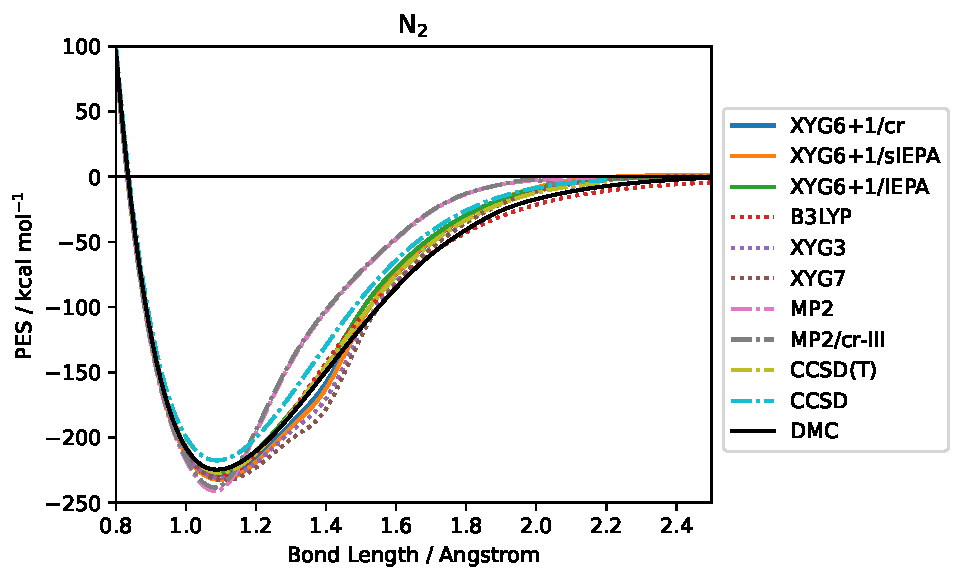
\includegraphics[width=0.7\textwidth]{assets/curve-N2-stab.pdf}
  \caption[\ce{N2} 解离曲线表现 (开壳层)]{各方法在 \ce{N2} 解离曲线的表现。参考态方法均在开壳层下优化到稳定。}
  \label{fig.2.curve-N2-stab}
\end{figure}

\begin{figure}[!h]
  \centering
  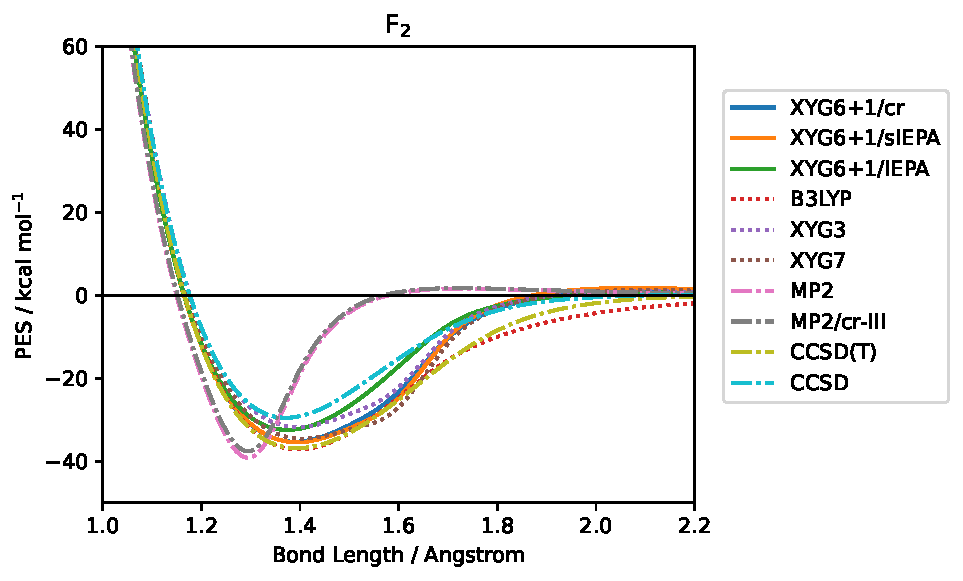
\includegraphics[width=0.7\textwidth]{assets/curve-F2-stab.pdf}
  \caption[\ce{F2} 解离曲线表现 (开壳层)]{各方法在 \ce{F2} 解离曲线的表现。参考态方法均在开壳层下优化到稳定。}
  \label{fig.2.curve-F2-stab}
\end{figure}

\begin{figure}[!h]
  \centering
  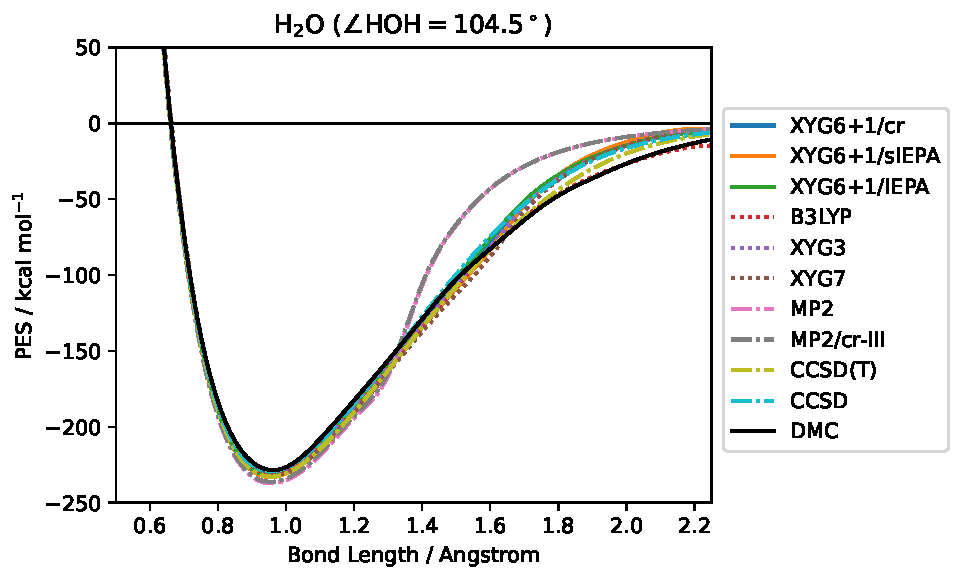
\includegraphics[width=0.7\textwidth]{assets/curve-H2O-stab.pdf}
  \caption[\ce{H2O} 解离曲线表现 (开壳层)]{各方法在 \ce{H2O} 解离曲线的表现。参考态方法均在开壳层下优化到稳定。}
  \label{fig.2.curve-H2O-stab}
\end{figure}

\begin{figure}[!h]
  \centering
  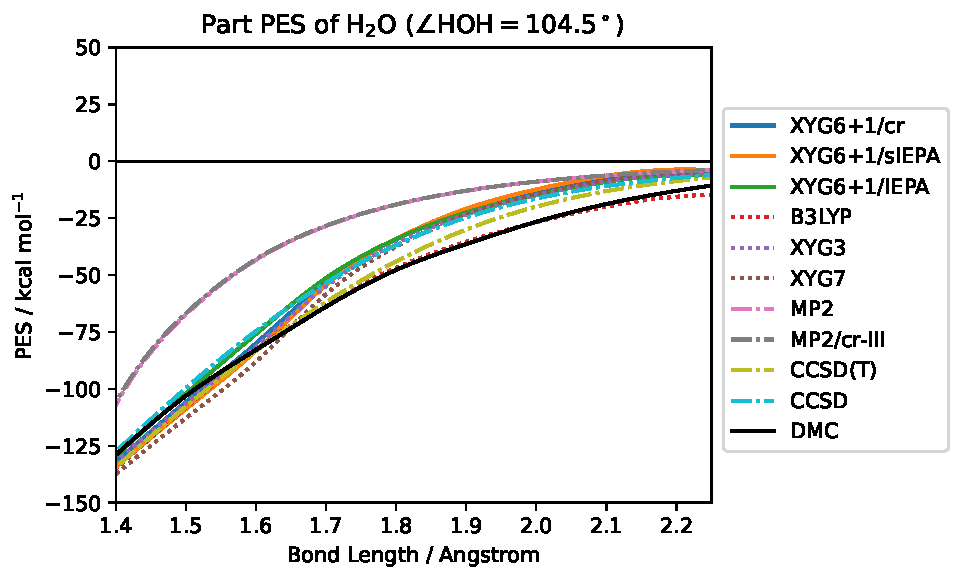
\includegraphics[width=0.7\textwidth]{assets/curve-H2O-part-stab.pdf}
  \caption[\ce{H2O} 解离曲线 1.4--2.25 \AA 段表现 (开壳层)]{各方法在 \ce{H2O} 解离曲线 1.4--2.25 \AA 段的表现。参考态方法均在开壳层下优化到稳定。}
  \label{fig.2.curve-H2O-part-stab}
\end{figure}

\begin{figure}[!h]
  \centering
  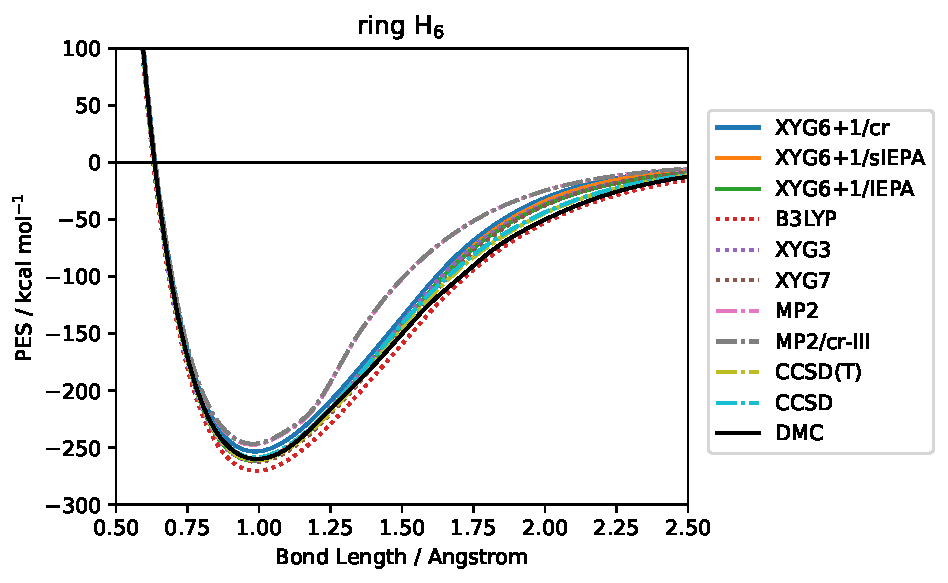
\includegraphics[width=0.7\textwidth]{assets/curve-H6-stab.pdf}
  \caption[\ce{H6} 解离曲线表现 (开壳层)]{各方法在 \ce{H6} 解离曲线的表现。参考态方法均在开壳层下优化到稳定。}
  \label{fig.2.curve-H6-stab}
\end{figure}

\pagebreak

\section{附录:电子对方法不具有正交不变性的说明}

对分子轨道的正交变换,会使得 Hartree-Fock 参考态对应分子轨道基的 Fock 矩阵并非对角矩阵。与 MP2 方法不同,本工作所考虑的电子对方法 MP2/cr 与 IEPA,其定义须基于正则 Hartree-Fock 轨道。因此,从定义上,MP2/cr 与 IEPA 方法等电子对方法,无法对非正则 Hartree-Fock 作计算,故而不存在正交不变性。

但是,对于正则 Hartree-Fock 能级简并的分子轨道,正交变换后的分子轨道仍然是正则的。此时,IEPA 或 MP2/cr 等电子对方法仍然是可以被定义的;从而,对简并分子轨道的正交变换不变性是可以讨论的。简并轨道可能源于下述四种情况:
\begin{enumerate}[nosep]
  \item 距离无穷远的两个完全等价体系产生的成对简并轨道;
  \item 因分子点群对称性而在二维不可约表示下产生的二重简并轨道;
  \item 因分子点群对称性而在三维不可约表示下产生的三重简并轨道;
  \item 偶然的能级简并。
\end{enumerate}
对于这些情形,我们将作简单的讨论与分析,并将表明本工作所考虑的电子对方法 (MP2/cr、IEPA) 依情况并非正交不变;同时,因简并分子轨道正交变换而导致的能量变化通常不严重,但也存在正交变换误差大于 0.5 eV 的情形。由于从表达式上,sIEPA 与 IEPA 具有相似的形式;因此,若 IEPA 并非正交不变,那么容易知道 sIEPA 也同样并非正交不变。但由于 sIEPA 引入了 erfc 形式的放缩函数,因此正交变换误差通常小于 IEPA。

这一小节的公式推演将基于自旋轨道;数值结果展现将基于闭壳层轨道。一些结论展示于表 \ref{tab.2.invariance-mp2cr-iepa}。该节的数值计算使用 cc-pVDZ 基组,程序使用 \textsc{PySCF} 与 \textsc{dh}。

\begin{table}[!ht]
\centering
\caption[MP2/cr 与 IEPA 在不同情形下的正交变换不变性]{MP2/cr 与 IEPA 在不同情形下能级简并轨道间的正交变换不变性。}
\label{tab.2.invariance-mp2cr-iepa}
\widetabular{
  \begin{tabular}{cccl}
  \toprule
  情形 & MP2/cr & IEPA & 情形描述   \\
  \midrule
  1  & 满足 & 不满足 & 无穷远两分子 \\
  2  & 满足 & 满足 & 二维不可约  \\
  3  & 满足 & 不满足 & 三维不可约  \\
  4  & 不满足 & 不满足 & 偶然简并  \\
  \bottomrule
  \end{tabular}
}{}
\end{table}

\subsection{MP2/cr 方法在完全分离体系下的正交变换不变性}

对于完全分离体系,即距离无穷远的分子 $A$ 与分子 $B$ 的复合物 $AB$,严格的复合物电子对方法相关能 $E_\textmt{c} (AB)$ 等于两个单体分子的能量之和 $E_\textmt{c} (A) + E_\textmt{c} (B)$。该性质在本工作中称为大小一致性。特别地,若 $A$ 与 $B$ 体系完全等价,那么就会因为完全分离的体系而产生成对的简并轨道,这些简并轨道的能量与单体 $A$ 或 $B$ 的轨道能量一致;在这些简并轨道的正交变换下,电子对相关能应当是不变的。

作为近似的相关能计算方法,对于这类完全分离体系问题,在 M{\o}ller-Plesset 微扰收敛的前提下,MP2 是大小一致且正交变换不变的\cite{Szabo-Ostlund.Dover.1996, Shavitt-Bartlett.Cambridge.2009};而 IEPA 方法依占据轨道的选取并非正交不变 (因此不是严格的大小一致),但仍然是大小可延展的\cite{Szabo-Ostlund.Dover.1996, Zhang-Scheffler.NJP.2016},即随着分离体系中的独立子体系的增多、相关能大致线性地增加。

这一小节将表明,对于 $A$ 与 $B$ 完全等价的情形,在特定的局域基下,它们构成的完全分离体系的复合物 $AB$ 的 MP2/cr 方法相关能 $E_\textmt{c}^\textmt{MP2/cr} (AB)$ 确实等于单体相关能之和 $E_\textmt{c}^\textmt{MP2/cr} (A) + E_\textmt{c}^\textmt{MP2/cr} (B)$。同时,在假定 $A, B$ 分子各自没有简并的占据轨道情形下,复合物 $AB$ 的一对占据简并轨道正交变换下能量不变。

\subsubsection{MP2/cr 方法因完全分离体系而简并的轨道下正交不变性}

令 $i, j, \cdots$ 与 $a, b, \cdots$ 为\textbf{单体} $A$ 或 $B$ 的占据与未占轨道。使用下角标 $A$ 与 $B$ 以区分轨道所在的分离单体。对于复合物 $AB$,若其分子轨道基选取为 $i_A, j_A, \cdots, \allowbreak a_A, b_A, \allowbreak i_B, j_B, \cdots, \allowbreak a_B, b_B$,则称其为\textbf{局域基}。由于 $A$ 与 $B$ 完全分离,因此局域基是 Hartree-Fock 的正则轨道。

为简化记号表述,这里省去成对电子能量 $e_{ij}^\textmt{MP2/cr}$ 与相关能 $E_\textmt{c}^\textmt{MP2/cr}$ 的上标 $\textmt{MP2/cr}$。

对于分子 $A$ 上的占据轨道 $l_A$ 与分子 $B$ 上的占据轨道 $l_B$,定义正交变换后的分子轨道 $\mathscr{l}_1$ 与 $\mathscr{l}_2$ 为
\begin{align}
  \label{eq.2.invariance-general}
  \begin{aligned}
    \mathscr{l}_1 &= \cos(\theta) l_A - \sin(\theta) l_B \\
    \mathscr{l}_2 &= \sin(\theta) l_A + \cos(\theta) l_B
  \end{aligned}
\end{align}
我们称 $\theta$ 为正交变换相位。特别地,在该段落中,我们仅对 $\theta = - \pi/4$ 的情形作讨论:
\begin{align}
  \label{eq.2.invariance-specific}
  \mathscr{l}_1 = \frac{1}{\sqrt{2}} (l_A + l_B), \quad \mathscr{l}_2 = \frac{1}{\sqrt{2}} (l_A - l_B)
\end{align}
除了 $l_A$ 与 $l_B$ 轨道作正交变换外,其余轨道均与局域基相同。这里称其为\textbf{离域基}。

首先简要表明 MP2/cr 方法在局域基下是大小一致的。简记分子轨道基的 ERI 张量 $\langle ij | ab \rangle$ 为 $g_{ij}^{ab}$,则对于分离的单体而言,对应式 (\ref{eq.2.eij-MP2cr}),成对电子 $ij$ 的相关能为
\begin{equation*}
  e_{ij} = \frac{1}{2} \sum_{ab} \frac{1}{N_{ij}} \frac{\big( g_{ij}^{ab} - g_{ij}^{ba} \big)^2}{D_{ij}^{ab}} = \frac{1}{2} \sum_{ab} \frac{1}{N_{ij}} \big( t_{ij}^{ab} \big)^2 D_{ij}^{ab}
\end{equation*}
MP2 激发张量 $t_{ij}^{ab}$ 是
\begin{equation*}
  t_{ij}^{ab} = \frac{g_{ij}^{ab} - g_{ij}^{ba}}{D_{ij}^{ab}}
\end{equation*}
MP2/cr 缩放比例 $N_{ij}$ 定义式在 (\ref{eq.2.Nij-MP2cr}) 已有表述。

对于复合物 $AB$ 的局域基,首先注意到 ERI 张量中,若有轨道分属于不同的原子,那么该张量元的值为零;即仅有类似于 $g_{i_A j_A}^{a_A b_A}$ 或 $g_{i_B j_B}^{a_B b_B}$ 的元素非零。可以得知的推论是,MP2 激发张量也仅有类似于 $t_{i_A j_A}^{a_A b_A}$ 或 $t_{i_B j_B}^{a_B b_B}$ 的元素非零;进而
\begin{gather*}
  N_{i_A j_A} = N_{i_B j_B} = N_{ij}, \quad N_{i_A j_B} = N_{i_A j_B} = 0 \quad (\forall i, j) \\
  e_{i_A j_A} = e_{i_B j_B} = e_{ij}, \quad e_{i_A j_B} = e_{i_A j_B} = 0 \quad (\forall i, j) \\
  E_\textmt{c} (AB) = \frac{1}{2} \sum_{i_A j_A} e_{i_A j_A} + \frac{1}{2} \sum_{i_B j_B} e_{i_B j_B} = \sum_{ij} e_{ij} = E_\textmt{c} (A) + E_\textmt{c} (B) \quad \text{(localized basis)}
\end{gather*}
因此容易表明,MP2/cr 在局域基下是大小一致的。

随后需要说明 MP2/cr 在离域基下的相关能与局域基是相同的。首先,$l_A$ 与 $l_B$ 的轨道能均为 $\varepsilon_l$;因此,对这两根轨道的正交变换后,得到的 $\mathscr{l}_1$ 与 $\mathscr{l}_2$ 轨道能仍然有
\begin{equation*}
  \varepsilon_{\mathscr{l}_1} = \varepsilon_{\mathscr{l}_2} = \varepsilon_l
\end{equation*}
对于离域基,占据轨道中并非 $\mathscr{l}_1$ 与 $\mathscr{l}_2$ 的部分,其结果与局域基完全一致;这部分的结果显然是相等的。因此,我们仅讨论涉及 $\mathscr{l}_1$ 与 $\mathscr{l}_2$ 的部分。对于 ${i_A \mathscr{l}_1}$ 电子对的情形 ($\forall i \neq l$),注意到对于 $\forall a, b$,
\begin{align*}
  g_{i_A \mathscr{l}_1}^{a_A b_A} &= \frac{1}{\sqrt{2}} g_{i_A l_A}^{a_A b_A} + \frac{1}{\sqrt{2}} g_{i_A l_B}^{a_A b_A} = \frac{1}{\sqrt{2}} g_{il}^{ab} \\
  t_{i_A \mathscr{l}_1}^{a_A b_A} &= \frac{1}{\sqrt{2}} \frac{g_{i_A l_A}^{a_A b_A} - g_{i_A l_A}^{b_A a_A}}{D_{il}^{ab}} = \frac{1}{\sqrt{2}} t_{il}^{ab}
\end{align*}
对于 $g_{i_A \mathscr{l}_2}^{a_A b_A}$ 与 $t_{i_A \mathscr{l}_2}^{a_A b_A}$ 有同样的结论。对于 $\mathscr{l}_1 \mathscr{l}_2$ 电子对的情形,注意到 ERI 张量的对称性 $g_{l_A l_A}^{a_A b_A} = g_{l_A l_A}^{b_A a_A}$,因此
\begin{align*}
  g_{\mathscr{l}_1 \mathscr{l}_2}^{a_A b_A} &= \frac{1}{2} g_{l_A l_A}^{a_A b_A} \\
  t_{\mathscr{l}_1 \mathscr{l}_2}^{a_A b_A} &= \frac{1}{2} \frac{g_{l_A l_A}^{a_A b_A} - g_{l_A l_A}^{b_A a_A}}{D_{il}^{ab}} = 0
\end{align*}
对于分子 $B$ 的情况也是类似的:
\begin{gather*}
  t_{i_B \mathscr{l}_1}^{a_B b_B} = - t_{i_B \mathscr{l}_2}^{a_B b_B} = \frac{1}{\sqrt{2}} t_{ij}^{ab} , \quad
  t_{\mathscr{l}_1 \mathscr{l}_2}^{a_B b_B} = 0
\end{gather*}

因此,对于 $\forall i, j \neq l$,
\begin{align*}
  N_{i_A j_A} &= 1 + \frac{1}{2} \sum_{\substack{k_A \neq l_A \\ a_A b_A}} \left( \big( t_{i_A k_A}^{a_A b_A} \big)^2 + \big( t_{j_A k_A}^{a_A b_A} \big)^2 \right) \\
  &\quad + \frac{1}{2} \left( \big( t_{i_A \mathscr{l}_1}^{a_A b_A} \big)^2 + \big( t_{i_A \mathscr{l}_2}^{a_A b_A} \big)^2 + \big( t_{j_A \mathscr{l}_1}^{a_A b_A} \big)^2 + \big( t_{j_A \mathscr{l}_2}^{a_A b_A} \big)^2 \right) \\
  &= 1 + \frac{1}{2} \sum_{\substack{k \neq l \\ ab}} \left( \big( t_{ik}^{ab} \big)^2 + \big( t_{jk}^{ab} \big)^2 \right) \\
  &\quad + \frac{1}{2} \left( \frac{1}{2} \big( t_{il}^{ab} \big)^2 + \frac{1}{2} \big( t_{il}^{ab} \big)^2 + \frac{1}{2} \big( t_{jl}^{ab} \big)^2 + \frac{1}{2} \big( t_{jl}^{ab} \big)^2 \right) \\
  &= 1 + \frac{1}{2} \sum_{kab} \left( \big( t_{ik}^{ab} \big)^2 + \big( t_{jk}^{ab} \big)^2 \right) \quad \text{(delocalized basis)}
\end{align*}
即对于 $\forall i, j \neq l$,缩放系数 $N_{i_A j_A}$ 不论是局域基还是离域基下,结果均相同。因此,可以证明成对电子 $i_A j_A$ 相关能也是一致的:
\begin{equation*}
  e_{i_A j_A} = \frac{1}{2} \sum_{ab} \frac{1}{N_{i_A j_A}} \big( t_{i_A j_A}^{a_A b_A} \big)^2 D_{ij}^{ab} = \frac{1}{2} \sum_{ab} \frac{1}{N_{ij}} \big( t_{ij}^{ab} \big)^2 D_{ij}^{ab} = e_{ij} \quad \text{(delocalized basis)}
\end{equation*}
上述结论对于分子 $B$ 同理。

对于 $\forall i \neq l$,首先注意到 MP2 激发张量中,相同占据轨道的元素是零,举例而言即 $t_{i_A i_A}^{a_A b_A} = 0$ 或 $t_{\mathscr{l}_1 \mathscr{l}_1}^{a_A b_A} = 0$ ($\forall i, a, b$);但同时需要注意到,回顾式 (\ref{eq.2.Nij-MP2cr}),对于 $AB$ 复合物而言,被求和的指标包括 $A$ 分子与 $B$ 分子的所有轨道,因此
\begingroup
\allowdisplaybreaks
\begin{align*}
  N_{i_A \mathscr{l}_1} &= 1 + \frac{1}{2} \sum_{\substack{k_A \neq l_A \\ a_A b_A}} \big( t_{i_A k_A}^{a_A b_A} \big)^2 + \frac{1}{2} \big( t_{i_A \mathscr{l}_1}^{a_A b_A} \big)^2 + \frac{1}{2} \big( t_{i_A \mathscr{l}_2}^{a_A b_A} \big)^2 \\
  &\quad + \frac{1}{2} \sum_{\substack{k_A \neq l_A \\ a_A b_A}} \big( t_{\mathscr{l}_1 k_A}^{a_A b_A} \big)^2 + \frac{1}{2} \sum_{\substack{k_B \neq l_B \\ a_B b_B}} \big( t_{\mathscr{l}_1 k_B}^{a_B b_B} \big)^2 + \frac{1}{2} \big( t_{\mathscr{l}_1 \mathscr{l}_1}^{a_A b_A} \big)^2 + \frac{1}{2} \big( t_{\mathscr{l}_1 \mathscr{l}_2}^{a_A b_A} \big)^2 \\
  &= 1 + \frac{1}{2} \sum_{\substack{k \neq l \\ ab}} \big( t_{ik}^{ab} \big)^2 + \frac{1}{4} \big( t_{il}^{ab} \big)^2 + \frac{1}{4} \big( t_{il}^{ab} \big)^2 \\
  &\quad + \frac{1}{4} \sum_{\substack{k \neq l \\ ab}} \big( t_{lk}^{ab} \big)^2 + \frac{1}{4} \sum_{\substack{k \neq l \\ ab}} \big( t_{lk}^{ab} \big)^2 + 0 + 0 \\
  &= 1 + \frac{1}{2} \sum_{kab} \left( \big( t_{ik}^{ab} \big)^2 + \big( t_{lk}^{ab} \big)^2 \right) \quad \text{(delocalized basis)}
\end{align*}
\endgroup
因此,对于 $\forall i \neq l$,缩放系数离域基下的 $N_{i_A \mathscr{l}_1}$ 与局域基下的 $N_{i_A l_A}$ 的结果、或者 $A$ 或 $B$ 单体的 $N_{ij}$ 相等。因此,
\begin{equation*}
  e_{i_A \mathscr{l}_1} = \sum_{a_A b_A} \frac{1}{N_{i_A \mathscr{l}_1}} \big( t_{i_A \mathscr{l}_1}^{a_A b_A} \big)^2 D_{il}^{ab} = \frac{1}{2} \sum_{ab} \frac{1}{N_{il}} \big( t_{il}^{ab} \big)^2 D_{il}^{ab} = \frac{1}{2} e_{il} \quad \text{(delocalized basis)}
\end{equation*}
从而,离域基下的成对电子能 $e_{i_A \mathscr{l}_1}$ 是单个分子的 $e_{il}$ 的一半。类似地可以表明,离域基下,
\begin{equation*}
  e_{i_A \mathscr{l}_2} = e_{i_B \mathscr{l}_1} = e_{i_B \mathscr{l}_2} = \frac{1}{2} e_{il} \quad \text{(delocalized basis)}
\end{equation*}

对于离域基下的占据电子对 $\mathscr{l}_1 \mathscr{l}_2$,注意到先前已表明 $t_{\mathscr{l}_1 \mathscr{l}_2}^{a_B b_B} = 0$ ($\forall a, b$),因此容易知道 $e_{\mathscr{l}_1 \mathscr{l}_2} = 0$。

因此,可以推知离域基下,复合物 $AB$ 的 MP2/cr 相关能为
\begin{align*}
  E_\textmt{c} (AB) &= \frac{1}{2} \sum_{i_A j_A \neq l_A} e_{i_A j_A} + \sum_{i_A \neq l_A} \big( e_{i_A \mathscr{l}_1} + e_{i_A \mathscr{l}_2} \big) \\
  &\quad + \frac{1}{2} \sum_{i_B j_B \neq l_B} e_{i_B j_B} + \sum_{i_B \neq l_B} \big( e_{i_B \mathscr{l}_1} + e_{i_B \mathscr{l}_2} \big) + e_{\mathscr{l}_1 \mathscr{l}_2} \\
  &= \frac{1}{2} \sum_{ij \neq l} e_{ij} + \sum_{i \neq l} e_{il} \\
  &\quad + \frac{1}{2} \sum_{ij \neq l} e_{ij} + \sum_{i \neq l} e_{il} + 0 \\
  &= \sum_{ij} e_{ij} = E_\textmt{c} (A) + E_\textmt{c} (B) \quad \text{(delocalized basis)}
\end{align*}
该离域基下的复合物 $AB$ 相关能与 $A$、$B$ 单体的相关能之和完全相等。

上述讨论表明,尽管离域基与局域基并不等价;但复合物 $AB$ 的能量,在相同能级轨道的式 (\ref{eq.2.invariance-specific}) 定义下的正交变换下是不变的。

尽管我们仅仅针对式 (\ref{eq.2.invariance-specific}) 的特殊情况,作正交不变性的说明;但可以预期,若针对因等同分离体系而简并的占据或非占轨道,作式 (\ref{eq.2.invariance-general}) 下各种角度 $\theta$ 的正交变换,相关能 $E_\textmt{c} (AB)$ 仍然不变。

\subsubsection{接近完全分离体系的正交变换误差数值表现}

与式 (\ref{eq.2.invariance-general}) 相同地,对于两个独立体系 $A$ 与 $B$,构造轨道 $\mathscr{i}_1, \mathscr{i}_2$ 为分子轨道 $i_A, i_B$ 的线性组合
\begin{align*}
  \mathscr{i}_1 &= \cos(\theta) i_A - \sin(\theta) i_B \\
  \mathscr{i}_2 &= \sin(\theta) i_A + \cos(\theta) i_B
\end{align*}
当正交变换相位 $\theta$ 变换到 $\pi/2$ 时,则恰好交换了 $i_A$ 与 $i_B$;因此我们仅需要考察 $\theta \in [0, \pi/2]$ 的区间。由于 MP2 容易被证明、MP2/cr 已经由上文说明在当前的正交变换下是不变的,因此可以预期这两种方法的正交变换误差严格为零。

\begin{figure}[!ht]
  \centering
  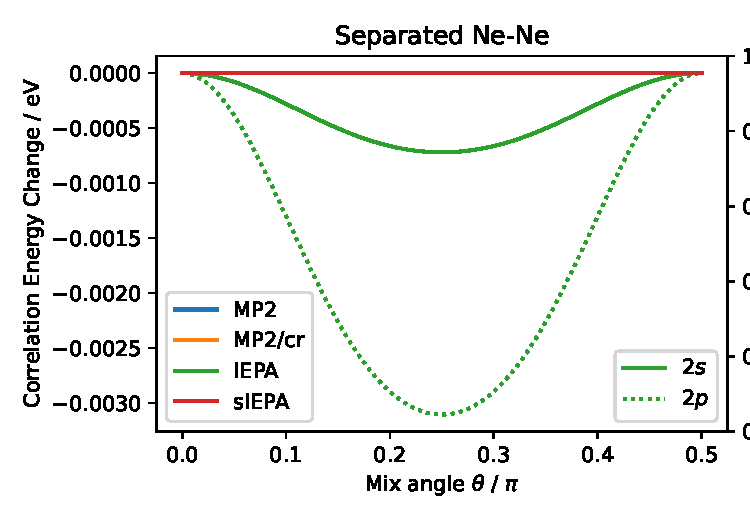
\includegraphics[width=0.6\textwidth]{assets/invar-sep-Ne.pdf}
  \caption[\ce{Ne2} 对称性简并轨道正交变换误差]{距离 100 \AA 的 \ce{Ne2} 的相关能随正交变换相位 $\theta$ 变化产生的误差。右下角图例表示被正交变换对应的单体分子轨道。该情形下 MP2、MP2/cr、sIEPA 的误差均为零或极其接近零,图上的曲线重合。}
  \label{fig.2.invar-sep-Ne}
\end{figure}

对于原子之间距离 100 \AA 的 \ce{Ne2} 体系,成对电子型相关能 $E_\textmt{c}^\textmt{EP}$ 依正交变换相位 $\theta$ 的变化情况展示于图 \ref{fig.2.invar-sep-Ne}。对于该体系,100 \AA 的距离可以看作相互没有影响 (复合物 MP2 相关能相比于两个 \ce{Ne} 原子相关能之和的误差是 \num{6e-8} eV,接近于自洽场能量收敛限)。对于该复合物的轨道正交变换,其导致的能量误差不超过 0.005 eV 或 0.1 kcal/mol;这种程度的影响并不是很大。作为比较,CISD 方法尽管是正交不变、但却是大小不可延展的;对于当前体系,距离 100 \AA 的 \ce{Ne2} 体系相关能与两个单独的 \ce{Ne} 原子相关能相差 0.246 eV。

注意到 sIEPA 在两个 \ce{Ne} 原子体系下接近于正交变换不变。这是因为 sIEPA 在 HOMO/LUMO gap 较大的情形下迅速退化到 MP2 (对于当前体系,sIEPA 与 MP2 能量的误差在机器精度即 $2^{-53}$ Hartree 量级)。因此,尽管 sIEPA 与 IEPA 有相似的表达形式、显然不是正交变换不变的,但其误差在 HOMO/LUMO gap 较大时,sIEPA 的正交变换误差会远小于 IEPA。

\begin{figure}[!ht]
  \centering
  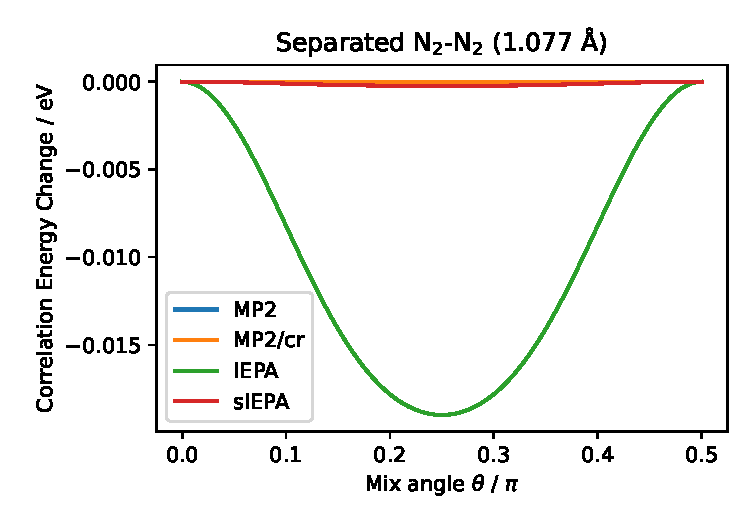
\includegraphics[width=0.6\textwidth]{assets/invar-sep-N2-1.pdf}
  \caption[\ce{N2} 对称性简并轨道正交变换误差 (键长 1.077 \AA)]{距离 100 \AA 的 \ce{N2} 的相关能随正交变换相位 $\theta$ 变化产生的误差。\ce{N2} 键长为 HF/cc-pVDZ 下平衡键长 1.077 \AA。右下角图例表示被正交变换对应的单体分子轨道。该情形下 MP2、MP2/cr、sIEPA 的误差均为零或极其接近零,图上的曲线重合。}
  \label{fig.2.invar-sep-N2-1}
\end{figure}

\begin{figure}[!ht]
  \centering
  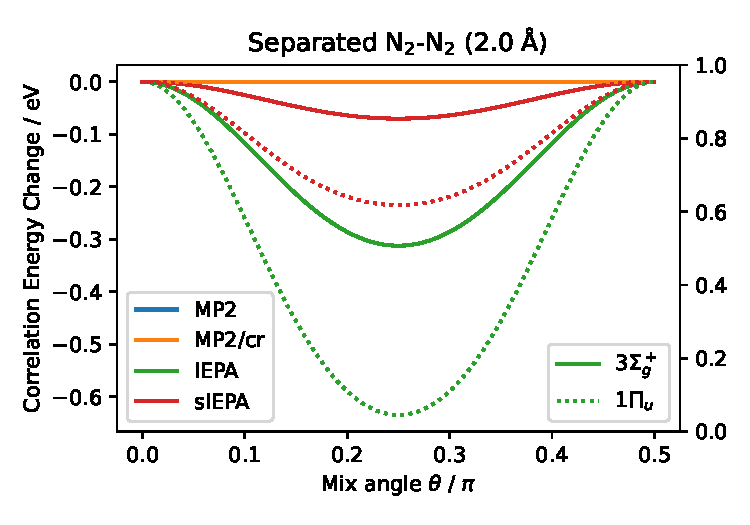
\includegraphics[width=0.6\textwidth]{assets/invar-sep-N2-2.pdf}
  \caption[\ce{N2} 对称性简并轨道正交变换误差 (键长 2.0 \AA)]{距离 100 \AA 的 \ce{N2} 的相关能随正交变换相位 $\theta$ 变化产生的误差。\ce{N2} 键长为 2.0 \AA。右下角图例表示被正交变换对应的单体分子轨道。该情形下 MP2、MP2/cr 的误差均为零,图上的曲线重合。}
  \label{fig.2.invar-sep-N2-2}
\end{figure}

如 Szabo 与 Ostlund 在 5.1.1 小节中对模型体系的讨论\cite{Szabo-Ostlund.Dover.1996},影响 IEPA 方法正交变换误差,受轨道能量差与双电子积分的共同影响。其中,轨道能差的影响较为关键;且被变换轨道与分子的 HOMO 或 LUMO 越接近,正交变换的误差就越大。对于两个 \ce{Ne} 原子体系而言,$2p$ 轨道的能级相比于 $2s$ 更高、与 LUMO 能级更接近,因此有更大的正交变换误差。从图 \ref{fig.2.invar-sep-N2-1} 与图 \ref{fig.2.invar-sep-N2-2} 上可以看出,对于两个 \ce{N2} 原子体系,若对其 HOMO 轨道 ($1 \symup{\Pi}_u$) 作正交变换,该情形更为明显。当 \ce{N2} 键长较短时,IEPA 的正交变换误差是较小的 $-0.019$ eV;但当 \ce{N2} 键长较长时,IEPA 的正交变换误差是较大的 $-0.635$ eV。同时,键长较长时,由于 HOMO/LUMO gap 也同时较小;因此 sIEPA 不再与 MP2 有相似的数值,从而显现出较大的正交变换误差。

\subsection{因点群对称性而简并的轨道下正交不变性}

\subsubsection{MP2/cr 该情形下正交不变性的简要说明}

MP2/cr 方法在数值计算结果上,对于因点群对称性而简并的轨道,显现出正交不变性。这里对 MP2/cr 方法在该情形下的正交不变性作不严格的说明。

首先,定义其中一种分子轨道基为 $i, j, \cdots, a, b, \cdots$。当前我们仅考虑占据轨道上的实正交变换;变换后的基为 $i', j', \cdots, a, b, \cdots$;变换后的张量上标波浪号。占据轨道的正交变换矩阵记为 $U_{i' i}$;若变换前的分子轨道到原子轨道线性组合的系数矩阵是 $C_{\mu i}$,则变换后的系数矩阵 $\tilde{C}_{\mu i'}$ 是
\begin{equation*}
  \tilde{C}_{\mu i'} = \sum_{i} C_{\mu i} U_{i' i}
  \quad \text{or} \quad
  \tilde{\mathbf{C}} = \mathbf{C} \mathbf{U}^\dagger
\end{equation*}
由于我们仅考虑因点群对称性而简并的轨道,因此 $U_{i' i}$ 矩阵除了简并轨道外,其余部分是单位矩阵。由于 ERI 张量对轨道的变换是线性的,因此容易表明对于下述定义的矩阵 $\mathscr{G}_{ij}$
\begin{equation*}
  \mathscr{G}_{ij} = \sum_{kab} g_{ik}^{ab} g_{jk}^{ab}
\end{equation*}
轨道变换后的矩阵有
\begin{equation*}
  \tilde{\mathscr{G}}_{i'j'} = \sum_{ij} U_{i' i} \mathscr{G}_{ij} U_{j' j}
  \quad \text{or} \quad
  \tilde{\symbfscr{G}} = \mathbf{U} \symbfscr{G} \mathbf{U}^\dagger
\end{equation*}
由于轨道变换不影响能级,因此对于下述定义的矩阵 $\mathscr{T}_{ij}$
\begin{equation*}
  \mathscr{T}_{ij} = \sum_{kab} t_{ik}^{ab} t_{jk}^{ab}
\end{equation*}
同样容易验证有
\begin{equation*}
  \tilde{\mathscr{T}}_{i'j'} = \sum_{ij} U_{i' i} \mathscr{T}_{ij} U_{j' j}
  \quad \text{or} \quad
  \tilde{\symbfscr{T}} = \mathbf{U} \symbfscr{T} \mathbf{U}^\dagger
\end{equation*}

回顾到 MP2/cr 的定义,式 (\ref{eq.2.Nij-MP2cr}) 所给出的缩放系数 $N_{ij}$ 同样可以写为
\begin{equation*}
  N_{ij} = 1 + \frac{1}{2} \big( \mathscr{T}_{ii} + \mathscr{T}_{jj} \big)
\end{equation*}
因此,尽管缩放系数的指标是成对电子 $ij$,但实际上仅由单指标的对角元 $\mathscr{T}_{ii}$ 确定。注意到我们变换的是二维或三维不可约表示下简并轨道;这些轨道之间在对称性上相互正交,因此 $\symbfscr{T}$ 矩阵在被变换的轨道上非对角元为零。同时,这些简并轨道出于相同的对称性,矩阵 $\symbfscr{T}$ 在这些简并轨道上的对角元数值相等,即是单位矩阵的倍数。在正交变换下,单位矩阵不变;因此,变换后的矩阵对角元 $\tilde{\mathscr{T}}_{i'i'}$ 对于被变换的简并轨道并未改变。对于没有被变换的轨道,正交变换矩阵 $U_{i'i}$ 在这些轨道上是单位矩阵,因此变换后的 $\tilde{\mathscr{T}}_{i' j'}$ 与变换前的 $\mathscr{T}_{ij}$ 相同。从而,正交变换后的 $\tilde{N}_{i'j'}$ 与变换前的 $N_{ij}$ 完全相同。

这里不对总相关能 $E_\textmt{c}^\textmt{MP2/cr}$ 的正交不变性作证明,但作补充说明与推测。成对电子能量 $e_{ij}^\textmt{MP2/cr}$ 在上述正交变换下,\textbf{并非}与 $\tilde{e}_{i'j'}^\textmt{MP2/cr}$ 相等;但对于 $i$ 代表被正交变换的基、$j$ 代表能级相同但未被正交变换的另一组基,那么对这些特定占据轨道的 $\sum_{ij} e_{ij}^\textmt{MP2/cr}$ 正交变换前后是不变的。从而,总相关能 $E_\textmt{c}^\textmt{MP2/cr}$ 在当前的正交变换下,也是不变的。

\subsubsection{点群对称性下简并轨道正交变换误差数值表现}

数值计算的体系选用 \ce{C4H4} 模型体系;该体系为 $T_d$ 点群,碳原子之间构成正四面体且键长为 2 \AA;氢原子与临近碳原子的键长为 2 \AA。该体系的电子共 14 对,占据排布是
$$
(1 A_1)^2 (1 T_2)^6 (2 A_1)^2 (2 T_2)^6 (3 A_1)^2 (3 T_2)^6 (1 E)^4
$$
我们分别考察 $3 T_d$ 和 $1 E$ 内部的电子正交变换。对于 $1E$ 的占据轨道,对其正交变换的方式在式 (\ref{eq.2.invariance-general}) 中定义;对于 $3 T_d$ 的占据轨道,我们仅旋转其中的两组,旋转过程也与式 (\ref{eq.2.invariance-general}) 一致。

\begin{figure}[!ht]
  \centering
  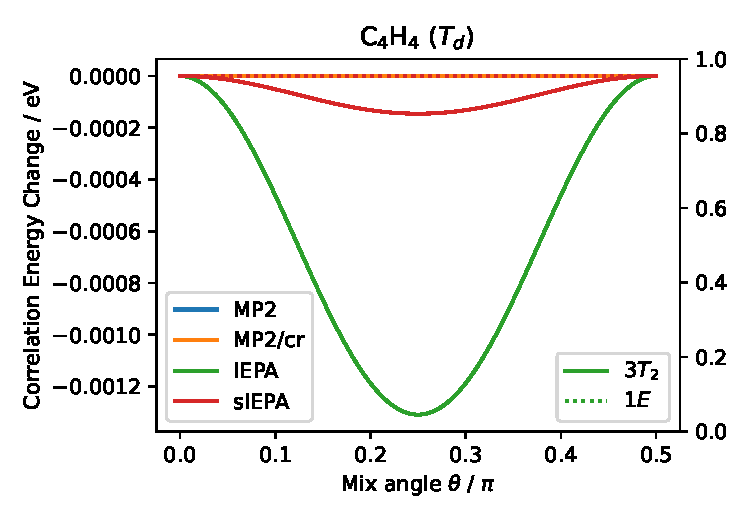
\includegraphics[width=0.6\textwidth]{assets/invar-sep-C4H4-1.pdf}
  \caption[$T_d$ 点群下 \ce{C4H4} 对称性简并轨道正交变换误差]{$T_d$ 点群下 \ce{C4H4} 的相关能随相同不可约表示简并轨道下正交变换相位 $\theta$ 变化产生的误差。右下角图例表示被正交变换对应的分子轨道。该情形下 MP2、MP2/cr 的误差,以及 $1E$ 轨道下所有方法的误差均为零,图上的曲线重合。}
  \label{fig.2.invar-sep-C4H4-1}
\end{figure}

对于当前情形,正交变换的相关能误差展示于图 \ref{fig.2.invar-sep-C4H4-1}。可以看到,对于二维不可约表示 $E$,所有方法都表现出了正交变换的不变性。但对于 $T_2$ 不可约表示,IEPA 与 sIEPA 方法存在一定的正交变换误差;其中,IEPA 方法误差最大为 $-0.0013$ eV,对于当前体系是相当小的数值。

\subsection{偶然能级简并的正交不变性}

这里仅使用数值表现,表明 MP2/cr 与 IEPA 均在偶然能级简并的轨道正交变换下存在误差。这里考察键长为 1.82116696109 \AA 的 \ce{CO} 分子。该分子的占据排布是
$$
(1 \symup{\Sigma}^+)^2 (2 \symup{\Sigma}^+)^2 (3 \symup{\Sigma}^+)^2 (4 \symup{\Sigma}^+)^2 (1 \symup{\Pi})^4 (5 \symup{\Sigma}^+)^2
$$
RHF/cc-pVDZ 基组下以能量 \num{1e-13} Hartree、轨道梯度 \num{1e-11} Hartree 为收敛限时,$1 \symup{\Pi}$ 轨道与 $5 \symup{\Sigma}^+$ 轨道的能级差小于 \num{1e-11} Hartree;在当前的分析中,该能极差可以认为接近于零,即这两种轨道是简并的。我们对其中一根 $1 \symup{\Pi}$ 轨道与 $5 \symup{\Sigma}^+$ 轨道作正交变换,变换相位在式 (\ref{eq.2.invariance-general}) 中定义。对于该情形,MP2/cr 与 IEPA 方法都展现出一定的正交变换误差,但误差数值不大于 0.005 eV。尽管在完全分离体系、以及二维或三维不可约简并轨道正交变换下,MP2/cr 展现出正交不变性;但该例子可以表明,MP2/cr 一般而言不具有正交不变性。

\begin{figure}[!ht]
  \centering
  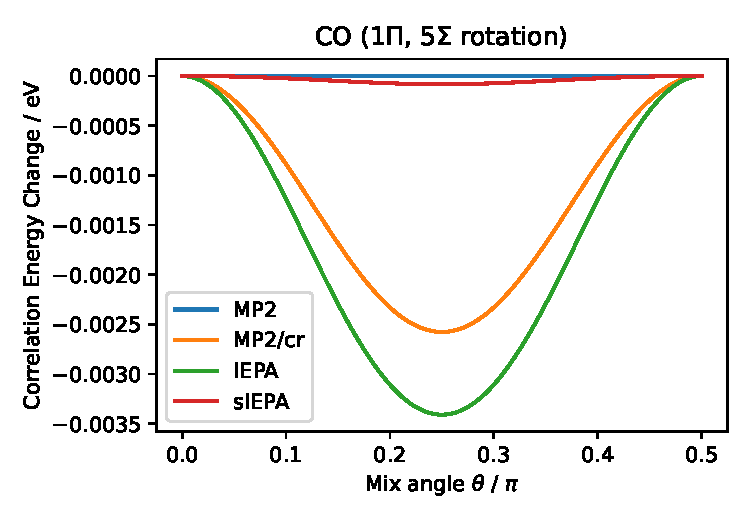
\includegraphics[width=0.6\textwidth]{assets/invar-sep-CO.pdf}
  \caption[\ce{CO} 偶然简并轨道正交变换误差]{\ce{CO} 分子的相关能在能级偶然简并的 $1 \symup{\Pi}$ 轨道与 $5 \symup{\Sigma}^+$ 轨道间依正交变换相位 $\theta$ 变化产生的误差。该情形下 MP2 的误差为零。}
  \label{fig.2.invar-sep-CO}
\end{figure}


\graphicspath{{../chap-03/}}
% !TEX root=./chap-03-dummy.tex

\section{双杂化泛函的电性质梯度理论与程序实现}

\subsection{引言}

表征技术是实验科学问题的重要分支之一。对于化学而言,经典的红外 (IR, \underline{I}nf\underline{r}ared)、紫外或可见光 (UV-Vis, \underline{U}ltra-\underline{V}iolet and \underline{Vis}able)、拉曼 (Raman)、核磁 (NMR, \underline{N}uclear \underline{M}agnetic \underline{R}esonance) 等表征手段被合称为“四大光谱”\footnote{“四大光谱”的说法并不是正式的。也有将拉曼光谱替换为质谱 (MS, \underline{M}ass \underline{S}pectrometry) 或 X 射线衍射谱 (XRD, \underline{X}-\underline{R}ay \underline{D}iffraction) 等。正文中说道计算化学对谱学问题有所帮助;但并不是所有谱学问题都与电子结构有紧密的关系、基于第一性的计算化学也未必能解决或解释所有谱学问题。例如质谱与分子构型关联度更大、X 射线衍射与晶格本身更有关、通过计算化学难以给出色谱的保留时间等。},在以有机化学为代表的分支学科中是必要的佐证手段。近年来,扫描隧道显微镜 (STM, \underline{S}canning \underline{T}unneling \underline{M}icroscopy)、原位红外 (\emph{in situ} IR)、表面增强拉曼 (SERS, \underline{S}urface-\underline{E}nhanced \underline{R}aman \underline{S}catting/\underline{S}pectroscopy)、扫描电化学显微镜 (SEM, \underline{S}canning \underline{E}lectron \underline{M}icroscopy) 等众多新兴表征手段兴起。由于其中的许多表征问题可以归结为电子结构或分子振动效应,因此可以或有希望通过第一性的计算化学方法计算得到,从而实验与理论或计算可以相互印证,推动化学学科的发展。

在前几章中已经表明密度泛函方法,特别是双杂化密度泛函近似,在基态能量计算上有较好的表现。我们预期在谱学计算上,双杂化密度泛函方法也能有良好的表现。为此,我们需要发展双杂化泛函的谱学计算方法。由于较多光谱问题 (包括 IR、Raman、NMR 等) 可以归结为偶极电场或磁场 $\pmb{\mathcal{E}}$ 下平衡态分子的基态能量 $E(\pmb{\mathcal{E}})$ 扰动问题,其中 $\pmb{\mathcal{E}}$ 为微扰外场;那么光谱的强度经常取决于导数量
\begin{equation}
  \lim_{|\pmb{\mathcal{E}}| \rightarrow 0} \frac{\mathrm{d}^n E(\pmb{\mathcal{E}})}{\mathrm{d} \pmb{\mathcal{E}}^n}
\end{equation}
或其导出量、或多种外场下的混合导数量。光谱问题也经常与分子振动有关;若上式的外场 $\pmb{\mathcal{E}}$ 替换为原子坐标移动向量,那么分子振动将化归为 $n = 2$ 即二阶导数问题。对于这类光谱计算问题,为通过计算化学手段进行模拟,我们需要对能量在外场下的梯度理论作研究与程序化。我们也称可以化归为梯度计算的光谱或振动问题为\textsf{梯度性质}问题。

双杂化泛函的梯度性质已经有先驱性的程序实现与测评\cite{Neese-Grimme.JCP.2007, Biczysko-Barone.JCTC.2010, Su-Xu.JCC.2013, Stoychev-Neese.JCTC.2018, Gu-Xu.JCTC.2021, Yan-Xu.JCTC.2022}。这些工作表明,双杂化泛函,特别是 xDH 型泛函,在分子振动、NMR 光谱预测等问题上有优异的表现。但目前的程序在计算双杂化解析梯度问题上,效率还一定提升空间。同时,考虑到双杂化泛函除了 MP2 型相关能外还有其它的杂化可能性;在理论推导与程序化过程中,也应尽量留出空间以容纳其它杂化形式。

在本章工作中,基于前人的工作\cite{Gerratt-Mills.JCP.1968, Gerratt-Mills.JCP.1968a, Pople-Binkley.IJQC.1979, Dykstra-Jasien.CPL.1984, Handy-Schaefer.JCP.1984, Handy-Simandiras.CPL.1985, Pulay-Saeboe.TCA.1986, Trucks-Bartlett.CPL.1988, Frisch-Pople.CP.1990, Frisch-Pople.CPL.1990, Frisch-Pople.CPL.1990a, Gauss-Bartlett.JCP.1992, Stanton-Bartlett.CPL.1992, Johnson-Frisch.CPL.1993, Head-Gordon-Head-Gordon.CPL.1994, Yamaguchi-Schaefer.Oxford.1994, Weigend-Haeser.TCA.1997, Aikens-Gordon.TCA.2003, Cammi-Frisch.TCA.2004, Distasio-Head-Gordon.JCC.2007, Neese-Grimme.JCP.2007, Biczysko-Barone.JCTC.2010, Su-Xu.JCC.2013, Ji-Jung.JCTC.2013, Bykov-Neese.MP.2015, Stoychev-Neese.JCTC.2018, Gu-Xu.JCTC.2021, Yan-Xu.JCTC.2022},将以电性质外场微扰为前提下,进行双杂化二阶梯度梯度的理论推演、与基于原子轨道基的程序化。\ref{sec.3.background} 节将介绍物理问题背景与程序化背景,以确定大体的技术线路。\ref{sec.3.theory} 节将介绍一般双杂化泛函电性质解析梯度理论。MP2 型泛函作为双杂化泛函的其中一个重要的分支,其在 RI 近似下解析静态极化率的 Python 代码在 CPU 上的实现细节将在 \ref{sec.3.program} 阐述,并作简单的效率测评。

\subsection{背景:记号定义}

\subsubsection{Einstein 求和记号}

出于简化公式表达,后文将对张量缩并大量使用变种的 Einstein 求和记号 (Einstein notation)。一些例子是
\begin{subequations}
\begin{align}
  \label{eq.einsum.1}
  (ia|jb) = \sum_{\mu \nu \kappa \lambda} C_{\mu i} C_{\nu a} (\mu \nu | \kappa \lambda) C_{\kappa j} C_{\lambda b}
  &\Rightarrow 
  (ia|jb) = C_{\mu i} C_{\nu a} (\mu \nu | \kappa \lambda) C_{\kappa j} C_{\lambda b} \\
  \label{eq.einsum.2}
  E_\mathrm{c}^\textsf{(2)} = - \frac{1}{4} \sum_{iajb} \frac{\big| \langle i j || a b \rangle \big|^2}{\varepsilon_i + \varepsilon_j - \varepsilon_a - \varepsilon_b}
  &\Rightarrow
  E_\mathrm{c}^\textsf{(2)} = - \frac{1}{4} \frac{\big| \langle i j || a b \rangle \big|^2}{\varepsilon_i + \varepsilon_j - \varepsilon_a - \varepsilon_b} \\
  \label{eq.einsum.3}
  \rho_g = \sum_{\mu \nu} D_{\mu \nu} \phi_{g \mu} \phi_{g \nu}
  &\Rightarrow
  \rho_g = D_{\mu \nu} \phi_{g \mu} \phi_{g \nu} \\
  \label{eq.einsum.4}
  L_{ai}^\textsf{xDH} = - (\varepsilon_a - \varepsilon_i) Z_{ai}^\textsf{xDH} - \sum_{bj} A_{ai, bj} Z_{bj}^\textsf{xDH}
  &\Rightarrow
  L_{ai}^\textsf{xDH} = - (\varepsilon_a - \varepsilon_i) Z_{ai}^\textsf{xDH} - A_{ai, bj} Z_{bj}^\textsf{xDH}
\end{align}
\end{subequations}
需要指出,这里的 Einstein 求和记号与物理中通常使用的记号不同\cite{Einstein-Einstein.AP.1916}。在物理中的 Einstein 求和记号依据对偶空间分上下标;以式 (\ref{eq.einsum.1}) 为例,若记 $g_{ij}^{ab} = (ia|jb)$,则通常物理的 Einstein 求和应写为:
\begin{equation*}
  g_{ij}^{ab} = C^\mu_i C^a_\nu g^{\nu \lambda}_{\mu \kappa} C^\kappa_j C^b_\lambda
\end{equation*}
物理中的 Einstein 求和,会将等式一侧任何重复出现的角标进行求和;但对于式 (\ref{eq.einsum.3}, \ref{eq.einsum.4}),我们所使用的变种的 Einstein 求和记号的等式右出现重复了两次的角标但并未被求和,而是对角标作元素乘法 (elementwise multiplication)。对于式 (\ref{eq.einsum.3}),角标 $g$ 并不处于 $\mu, \nu$ 所在的对偶空间,因此没有物理中 Einstein 记号的对应写法。对于式 (\ref{eq.einsum.4}),由于我们一般要求自洽场计算是正则的 (canonical),即 Fock 矩阵 $F_{pq}$ (或依物理的 Einstein 记号记为 $F_p^q$) 是对角矩阵且其对角元 $\varepsilon_p$ 被称为轨道能;因此式 (\ref{eq.einsum.4}) 在物理的 Einstein 记号下是
\begin{equation*}
  (L_a^i){}^\textsf{(2)} = - F_a^b (D_b^i){}^\textsf{(2)} - F_j^i (D_a^j){}^\textsf{(2)} - A_{aj}^{ib} (D_b^j){}^\textsf{(2)}
\end{equation*}
本文档的公式所使用的变种 Einstein 求和记号,会比较接近于具体程序实现时的情形 (\verb|NumPy.einsum| 或 \verb|opt_einsum.contract|),并允许打破一些物理记号的限制。

\subsubsection{记号与角标}

本工作通常使用下述记号:
\begin{itemize}[nosep]
  \item 下标 $\mu, \nu, \kappa, \lambda, \eta, \xi$:原子轨道 (基轨道);
  \item 下标 $i, j, k, l$:占据分子轨道;
  \item 下标 $a, b, c$:非占分子轨道;
  \item 下标 $p, q, r, s, m$:任意分子轨道;
  \item 下标 $P, Q, R, S$:RI 辅助基轨道;
  \item 上下标 $\mathbb{A}, \mathbb{B}$:外场微扰量、被求导量;
  \item 下标或向量 $A, B, M$:原子核;
  \item 下标 $w, t$:坐标分量 (用于指代 $x, y, z$);
  \item 下标 $\rho, \gamma$:密度与梯度导出量;
  \item 上标 $\mathrm{n}$:非变分泛函 (\underline{N}on-variational,相对于自洽场泛函);
  \item 上标 $\mathrm{S}$:\underline{S}keleton 导数;
  \item 上标 $\mathrm{U}$:轨道旋转导数 (\underline{U}nitary Transformation,涉及 U 矩阵 (\ref{eq.def.U}) 的导数);
  \item 上标 $\sigma, \varsigma$:自旋 (指代 $\alpha$ 或 $\beta$);
  \item 临时记号 $\mathscr{T}$ 作为算法中间张量,仅在局部的前后文中有意义。
\end{itemize}

本工作在不作额外说明的情形时,将讨论闭壳层 (closed-shell) 实现;对于开壳层问题,不同自旋下的轨道通过上标横线区分 ($p$ 表示 $\alpha$ 自旋、$\bar p$ 表示 $\beta$ 自旋),矩阵或张量则将上标具体的自旋。

本工作的全部理论推导与程序实现使用实数。为简化公式表达,大多数情形将不使用复共轭记号 (上标星号 $*$)。通常使用 $\phi_\mu (\bm{r})$ 表示原子轨道 $\mu$ 在空间坐标 $\bm{r}$ 下的函数表达式。对于 DFT 格点积分,若记坐标在角标 $g$ 下的离散格点为 $\bm{r}_g$,那么也经常用 $\phi_{g \mu}$ 作为二阶张量表示空间格点下的原子轨道函数值 $\phi_\mu (\bm{r}_g)$。

\subsubsection{部分常用表达式}

本工作使用到的电子积分有:
\begin{itemize}[nosep]
  \item 重叠积分 $S_{\mu \nu}$ (overlap):
        \begin{equation}
          S_{\mu \nu} := \int \phi_\mu (\bm{r}) \phi_\nu (\bm{r}) \, \mathrm{d} \bm{r}
        \end{equation}
  \item 无外场下的外势积分 $V_{\mu \nu}$:
        \begin{equation}
          V_{\mu \nu} := \int \phi_\mu (\bm{r}) \frac{- Z_A}{|\bm{r} - \bm{A}|} \phi_\nu (\bm{r}) \, \mathrm{d} \bm{r}
        \end{equation}
        上式对原子核角标 $A$ 求和;$Z_A$ 是原子单位下的原子核电荷数。
  \item 无外场下单电子积分 $h_{\mu \nu}$ (Hamiltonian core):
        \begin{equation}
          h_{\mu \nu} := S_{\mu \nu} + V_{\mu \nu}
        \end{equation}
  \item 四中心双电子互斥积分 $(\mu \nu | \kappa \lambda)$ (4c-2e ERI, 4-\underline{c}enter 2-\underline{e}lectron \underline{E}lectron \underline{R}epulsion \underline{I}ntegral):
        \begin{equation}
          (\mu \nu | \kappa \lambda) := \iint \phi_\mu (\bm{r}_1) \phi_\nu (\bm{r}_1) \frac{1}{r_{12}} \phi_\kappa (\bm{r}_2) \phi_\lambda (\bm{r}_2) \, \mathrm{d} \bm{r}_1 \mathrm{d} \bm{r}_2
        \end{equation}
        该积分也称传统双电子积分 conventional ERI 或简记为 conv ERI。
  \item 三中心双电子互斥积分 $(\mu \nu | P)$ (3c-2e ERI):
        \begin{equation}
          (\mu \nu | P) := \iint \phi_\mu (\bm{r}_1) \phi_\nu (\bm{r}_1) \frac{1}{r_{12}} \phi_P (\bm{r}_2) \, \mathrm{d} \bm{r}_1 \mathrm{d} \bm{r}_2
        \end{equation}
  \item 双中心双电子互斥积分 $J_{PQ}$ (2c-2e ERI):
        \begin{equation}
          J_{PQ} := \iint \phi_P (\bm{r}_1) \frac{1}{r_{12}} \phi_Q (\bm{r}_2) \, \mathrm{d} \bm{r}_1 \mathrm{d} \bm{r}_2
        \end{equation}
\end{itemize}

除了密度矩阵、弛豫张量等情形外,其它的原子轨道基下的张量,转换到分子轨道基时总是乘以轨道系数矩阵 $C_{\mu p}$。以原子与分子轨道混合基下的三中心双电子积分 $(\mu i | P)$ 为例,
\begin{equation*}
  (\mu i | P) = (\mu \nu | P) C_{\nu i}
\end{equation*}

在不引起歧义的情况下,将使用矩阵或张量元素指代矩阵或张量本身,例如用 $D_{\mu \nu}$ 表示完整的自洽场密度矩阵 $\mathbf{D}$。

本工作常用到的表达式有
\begin{itemize}[nosep]
  \item 闭壳层自洽场密度矩阵 $D_{\mu \nu}$ 与 $D_{pq}$:
        \begin{alignat}{10}
          \label{eq.def.dm-scf-closed}
          D_{\mu \nu} &:= C_{\mu p} D_{pq} C_{\nu q} = 2 C_{\mu i} C_{\nu i} \quad &&\text{(closed-shell)} \\
          D_{pq} &:= 2 \delta_{pq} \delta_{p \in \mathrm{occ}} \quad &&\text{(closed-shell)}
        \end{alignat}
        上式的 $\delta_{p \in \mathrm{occ}}$ 是指当 $p$ 属于占据轨道时取 1、不属于占据轨道时取 0。后文将涉及其它类型的密度 (譬如 xDH 约化密度 $D_{pq}^{\textsf{xDH}, \textsf{RDM}}$ 与弛豫密度 $D_{pq}^{\textsf{xDH}}$),需要上标类型以作区分;除自旋记号、没有额外上标的密度,均视为自洽场密度。
  \item 开壳层自洽场密度矩阵 $D_{\mu \nu}^\alpha$ 与 $D_{pq}$:
        \begin{align}
          D_{\mu \nu}^\alpha &:= C_{\mu p} D_{pq} C_{\nu q} = C_{\mu i} C_{\nu i} \\
          D_{pq} &:= \delta_{pq} \delta_{p \in \mathrm{occ}}
        \end{align}
        对于 $\beta$ 自旋的情形是类似的:
        \begin{align}
          D_{\mu \nu}^\beta &:= C_{\mu \bar p} D_{\bar p \bar q} C_{\nu \bar q} = C_{\mu \bar i} C_{\nu \bar i} \\
          D_{\bar p \bar q} &:= \delta_{\bar p \bar q} \delta_{\bar p \in \mathrm{occ}}
        \end{align}
        开壳层自洽场的总密度矩阵记为 $D_{\mu \nu} = D_{\mu \nu}^\alpha + D_{\mu \nu}^\beta$。
  \item 双杂化泛函总能量 $E^\textsf{tot}$:
        \begin{equation}
          \label{eq.def-E-tot}
          E^\textsf{tot} := E^\textsf{core} [\mathbf{D}] + E^\textsf{ERI} [\mathbf{D}] + E^\textsf{DFA} [\mathbf{D}] + E^\textsf{PT} [\mathbf{C}] + E^\textsf{non-elec} \\
        \end{equation}
        对于杂化泛函,$E^\textsf{PT} [\mathbf{C}]$ 取零值。每个能量分项的计算将在下面列举。需要指出,上式表述的是目前流行的双杂化泛函的能量表达式,而并非定义式。
  \item 单电子积分能量 $E^\textsf{core} [\mathbf{D}]$:
        \begin{equation}
          E^\textsf{core} [\mathbf{D}] := h_{\mu \nu} D_{\mu \nu}
        \end{equation}
  \item 双电子积分能量 $E^\textsf{ERI} [\mathbf{D}]$:
        \begin{equation}
          \label{eq.def.eng-eri}
          E^\textsf{ERI} [\mathbf{D}] := E^\textsf{J} [\mathbf{D}] + c_\mathrm{x} E_\mathrm{x}^\textsf{exact} [\mathbf{D}] + c_\mathrm{x}^\textsf{LR} E_\mathrm{x}^\textsf{LR} [\mathbf{D}]
        \end{equation}
        其中,$E^\textsf{J} [\mathbf{D}]$ 是库伦能\footnote{事实上,尽管本工作对双电子积分 $(\mu \nu | \kappa \lambda)$ 作近似;但该近似是 \ref{sec.rijk-rimp2-efficiency} 小节 RI 近似,它使用了计算复杂度为 $O(n_\mathrm{AO}^2 n_\mathrm{aux}) \sim O(N^3)$ 的三中心双电子积分 $(\mu \nu | P)$,因而在实际程序中仍然使用密度矩阵 $\mathbf{D}$ 描述库伦能。库伦能在程序实现上,确实可以通过密度格点 $\rho$ 而非具有更多细节的密度矩阵 $\mathbf{D}$ 计算实现、且计算复杂度为更小的 $O(N^2)$\cite{Toivanen-Sundholm.PCCP.2015};但我们的主要研究对象是双杂化泛函,在交换能 $E_\mathrm{x}^\textsf{exact}$ 与微扰能 $E^\textsf{PT}$ 难以使用密度格点 $\rho$ 进行计算的情况下,在程序实现中使用密度矩阵 $\mathbf{D}$ 以描述库伦能相信是可以接受的。}
        \begin{equation}
          \label{eq.def.ej}
          E^\textsf{J} [\mathbf{D}] = J[\rho] := \frac{1}{2} D_{\mu \nu} (\mu \nu | \kappa \lambda) D_{\kappa \lambda}
        \end{equation}
        $c_\mathrm{x}$ 特指严格交换系数 (区别于其它 DFA 交换系数),$E_\mathrm{x}^\textsf{exact} [\mathbf{D}]$ 是严格交换能
        \begin{equation}
          E_\mathrm{x}^\textsf{exact} [\mathbf{D}] = E_\mathrm{x}^\textsf{exact} [\rho] := - \frac{1}{2} D_{\mu \nu}^\sigma (\mu \lambda | \kappa \nu) D_{\kappa \lambda}^\sigma
        \end{equation}
        对于闭壳层问题,严格交换能可以写为
        \begin{equation}
          E_\mathrm{x}^\textsf{exact} [\mathbf{D}] := - \frac{1}{4} D_{\mu \nu} (\mu \lambda | \kappa \nu) D_{\kappa \lambda} \quad \text{(closed-shell)}
        \end{equation}
        部分泛函在交换能部分考虑了长短程效应;长程 (LR, \underline{L}ong-\underline{R}ange) 部分能量 $E_\mathrm{x}^\textsf{LR}$ 的双电子除了积分算符通常是 $\mathrm{erf} (\mu r_{12}) / r_{12}$\footnote{$\mu$ 是长程矫正的参数,通常小于 1。对于长程矫正作用,使用误差函数 $\mathrm{erf} (\mu r_{12}) / r_{12}$ 是常见且最多程序实现的方法;但除此之外,Yukawa 衰减算符 $\mathrm{exp} (-\mu r_{12}) / r_{12}$\cite{Savin-Flad.IJQC.1995} 与 $\mathrm{terf}$ 函数 $$\mathrm{terf} (r, r_0) := \frac{1}{2} \left( \mathrm{erf} \left(\frac{r - r_0}{\sqrt{2} r_0}\right) + \mathrm{erf} \left(\frac{r + r_0}{\sqrt{2} r_0}\right) \right)$$ 所构成的衰减算符 $\mathrm{terf} (-\mu r_{12}) / r_{12}$\cite{Goldey-Head-Gordon.PCCP.2013},也是其它可能使用到的长程矫正方案。},在计算、程序调用、张量分解等具体的程序实现上等同于严格交换能 $E_\mathrm{x}^\textsf{exact}$\footnote{需要指出,这只是双电子能量积分的一种表达方法。以 Cammi 等\cite{Cammi-Frisch.TCA.2004}对溶剂化模型下 MP2 二阶梯度理论为例,该文将电子效应诱导的溶剂化能量与双电子积分能量合并处理;而溶剂化能量的计算本身是不具有双电子积分。同时,在以较为抽象的层面上推导二阶梯度问题时,DFA 格点积分能量 $E^\textsf{DFA} [\mathbf{D}]$ 与双电子积分有类似的推演过程;因此从梯度理论的角度来讲,拆分双电子积分能量 $E^\textsf{ERI}$ 与 DFA 格点积分能量 $E^\textsf{DFA}$ 是人为的。在本工作中,我们不涉及溶剂化、基于密度的长程弥散矫正等其它无法简单纳入单电子积分能量的贡献;因此从程序实现方便、或计算量差异的角度,拆分了双电子积分能量与 DFA 格点积分能量。}。
  \item DFA 格点积分能量 $E^\textsf{DFA} [\mathbf{D}]$\footnote{区别于 DFA 近似总能量 $E^\textsf{tot}$。} 用以处理“Jacob 阶梯”上 1--3 阶 (LDA, GGA, meta-GGA) 交换相关能;它可以表示为对空间的积分
        \begin{equation}
          E^\textsf{DFA} [\mathbf{D}] := \int f[\rho, \gamma, \tau, \nabla^2 \rho, \cdots] \rho \, \mathrm{d} \bm{r}
        \end{equation}
        上式的 $f$ 若看作关于电子坐标 $\bm{r}$ 的函数,则其物理意义是在 $\bm{r}$ 处每个电子所具有的能量分布。$f$ 的具体表达式,取决于不同密度泛函所作不同的近似。其中,$\gamma$ 为 GGA 所用到的密度梯度导出量
        \begin{equation}
          \gamma := \nabla \rho \cdot \nabla \rho
        \end{equation}
        需要指出,动能密度 $\tau$ 导出自 Kohn-Sham 占据轨道 $\phi_i$ 而非密度 $\rho$ 本身,从而 $\tau$ \alert{引用第一章公式} 需要通过密度矩阵 $\mathbf{D}$、而非密度 $\rho$ 导出\footnote{对于 GGA 与 LDA,其能量或高阶导数确实是通过密度格点 $\rho$ 本身导出。以密度矩阵 $\mathbf{D}$ 作为参数不影响后文讨论;见库伦能定义式 (\ref{eq.def.ej}) 的脚注。}。因此在本工作中,为容许 meta-GGA 的程序实现,我们将 $E^\textsf{DFA}$ 视作密度矩阵 $\mathbf{D}$ 的泛函。在程序实现中,空间积分将化为格点积分求和式:
        \begin{equation}
          E^\textsf{DFA} \simeq w_g f_g \rho_g
        \end{equation}
        其中,$w_g$ 是空间坐标 $\bm{r}_g$ 下的格点积分权重、$f_g$ 与 $\rho_g$ 是能量分布函数与电子云密度在空间坐标 $\bm{r}_g$ 下的数值。
  \item 微扰能量 $E^\textsf{PT}[\mathbf{C}]$ 是双杂化泛函中的高阶近似部分。由于目前流行的杂化形式是 MP2 型相关能,因此这里统称为微扰能;但它也可以代表 IEPA 型相关能、RPA 型相关能等其它种类能量贡献项。一般来说,微扰能量 $E^\textsf{PT}$ 不纳入自洽场计算中,且并非密度矩阵 $\mathbf{D}$ 而是作为自洽场结果的轨道系数 $\mathbf{C}$ 的泛函。
  \item 无外场下的非电子效应能量 $E^\textsf{non-elec}$:
        \begin{equation}
          E^\textsf{non-elec} := \frac{1}{2} \frac{Z_A Z_B}{r_{AB}}
        \end{equation}
        其中,距离 $r_{AB}$ 定义为
        \begin{equation*}
          r_{AB} :=
          \begin{cases}
              | \boldsymbol{A} - \boldsymbol{B} | & A \neq B \\
              + \infty & A = B
          \end{cases}
        \end{equation*}
\end{itemize}

\subsubsection{xDH 型自洽场泛函与能量泛函}

xDH 型泛函分别对自洽场与总能量使用两种泛函形式;我们分别称之为\textsf{自洽场泛函}与\textsf{能量泛函}。由于 xDH 型泛函最终的能量并非通过变分得到,我们也称能量泛函为非变分泛函。自洽场是对下述能量求取分子轨道系数 $C_{\mu i}$ 的变分极小得到:
\begin{equation}
  \label{eq.def.eng-SCF}
  E^\textsf{SCF} = E^\textsf{core} [\mathbf{D}] + E^\textsf{ERI} [\mathbf{D}] + E^\textsf{DFA} [\mathbf{D}] + E^\textsf{non-elec}
\end{equation}
能量泛函部分项使用上标 $\mathrm{n}$ 进行区分;将自洽场给出的分子轨道系数 $C_{\mu p}$ 代入下式得到 xDH 能量:
\begin{equation}
  \label{eq.def.eng-xDH}
  E^\textsf{xDH} = E^\textsf{core} [\mathbf{D}] + E^{\mathrm{n}, \textsf{ERI}} [\mathbf{D}] + E^{\mathrm{n}, \textsf{DFA}} [\mathbf{D}] + E^\textsf{PT} [\mathbf{C}] + E^\textsf{non-elec}
\end{equation}
其中,$E^\textsf{core} [\mathbf{D}]$ 与 $E^\textsf{non-elec}$ 对于能量泛函和自洽场泛函没有区别。微扰能 $E^\textsf{PT} [\mathbf{C}]$ 仅在能量泛函出现;出于行文便利,将不对其作 $\mathrm{n}$ 的上标区分。为了后文讨论上的方便,我们额外定义 $E^{\mathrm{n}, \textsf{hyb}}$ 作为 $E^\textsf{xDH}$ 中,仅与密度矩阵 $\mathbf{D}$ 依赖的所有项之和:
\begin{equation}
  \label{eq.def.eng-n-hyb}
  E^{\mathrm{n}, \textsf{hyb}} := E^\textsf{core} [\mathbf{D}] + E^{\mathrm{n}, \textsf{ERI}} [\mathbf{D}] + E^{\mathrm{n}, \textsf{DFA}} [\mathbf{D}]
\end{equation}

需要补充的是,bDH 型泛函是当 xDH 型泛函的 $E^{\mathrm{n}, \textsf{ERI}} = E^\textsf{ERI}$、$E^{\mathrm{n}, \textsf{DFA}} = E^\textsf{DFA}$ 时的退化版本。bDH 型泛函由于仍然存有 $E^\textsf{PT} [\mathbf{C}]$ 一项,因此总能量泛函与 xDH 同样都是通过非变分途径计算得来。在目前的程序实现上,我们不需要区分 bDH 与 xDH 两者。

\subsubsection{导数记号与耦合微扰}

本工作将依是否存在耦合微扰 (CP, \underline{C}oupled \underline{P}erturbed),分为 Skeleton 导数 (骨架导数,部分文献也称为 core 导数即核导数)、轨道旋转导数、与一般的全导数。对于导数记号,在不引起歧义的情况下,
\begin{itemize}[nosep]
  \item 以分数形式描述的导数,$\frac{\mathrm{d}}{\mathrm{d} \mathbb{A}}$ 表示全导数,$\frac{\partial}{\partial \mathbb{A}}$ 表示偏导数;
  \item 以简写形式描述的导数,$\partial_\mathbb{A}$ 记号是\textsf{全导数} $\frac{\mathrm{d}}{\mathrm{d} \mathbb{A}}$ 的简记 (并非偏导数的含义,这是为了字母 $\mathrm{d}$ 被认为是变量);对性质量 $\mathbb{A}$ 的偏导数称为 Skeleton 导数并记为 $\partial_\mathbb{A}^\mathrm{S}$;涉及轨道系数的导数记为 $\partial_\mathbb{A}^\mathrm{U}$。$\partial_\mathbb{A}^\mathrm{S}$ 与 $\partial_\mathbb{A}^\mathrm{U}$ 将在这一小节的后文定义。
\end{itemize}

以总能量为例,在\textsf{特定的}外加微扰 $\mathbb{A}$ 与轨道系数 $\mathbf{C}$ 下,其能量记为 $E^\textsf{xDH} (\mathbb{A}, \mathbf{C})$。对于 xDH 型泛函,轨道系数是通过自洽场泛函得到;该轨道系数是随外加微扰而变化的\footnote{在本工作中,我们假定轨道系数随外加微扰是可以变化的,进而定义 U 矩阵 (\ref{eq.def.U}) 以描述轨道扰动情况\cite{Handy-Schaefer.JCP.1984}。尽管这一小节明确分别定义了对微扰外场与对分子轨道的偏导数,但当能量项的计算比较复杂时、或导数阶数高时,分子轨道系数对微扰外场的依赖性会增加推导难度。

另一类做法是完全避免使用 U 矩阵,而将轨道系数 $C_{\mu p}$、自洽场方程 (\ref{eq.SCF-working-equation}) 的 Lagrange 乘子 $\varepsilon_{pq}$、弛豫密度矩阵 $D_{pq}^\textsf{xDH}$ 作为自洽场方程 (\ref{eq.SCF-working-equation}) 的 Lagrange 乘子、加权密度矩阵 $W_{pq}^\textsf{xDH}$ 作为正交条件 (\ref{eq.constraint.ortho}) 的 Lagrange 乘子,这些变量都作为新构造的 Lagrangian 的参数;从而对该 Lagrangian 作梯度推演\cite{Helgaker-Joergensen.TCA.1989, Burow-Eshuis.JCTC.2014}。通过这个大量利用 Lagrange 乘子的方法,弛豫密度与能量加权密度矩阵都是自然定义的,而不需要像本工作以 Skeleton 梯度 (\ref{eq.collary.rdm-definition}) 定义 (难以通过波函数确定的、非变分方法的) 约化密度、以 Z-Vector 方程 (\ref{eq.Z-vector}) 进一步定义弛豫密度这样绕弯子的做法。同时,该推导途径也不需要特意引入作为数学技巧的 Z-Vector 方法 (\ref{eq.Z-vector-contrib-to-eng-deriv}) 与交换定理 (\ref{eq.interchange-theorem});且不需要考虑因轨道能级简并,而产生在强的正则自洽场条件 (\ref{eq.constraint.canonical-SCF}) 下,U 矩阵部分矩阵元数值不稳定的情形 (\ref{eq.unstable-Uij})。但该推导途径在目前大量涉及 MP2 型相关能的二阶梯度推演与计算中不是主流,且不会因其推演方式不同而给出更简洁或更高效的公式与程序;因此我们的工作仍然依主流的方法,使用 U 矩阵。\label{footnote.full-lagrangian}}:
\begin{equation*}
  \mathbf{C}^\textsf{SCF} (\mathbb{A}) := \arg \min_\mathbf{C} E^\textsf{SCF} (\mathbb{A}, \mathbf{C}) \quad \text{(with eq (\ref{eq.constraint.ortho}) satisfied)}
\end{equation*}
从而,实际的 xDH 能量不仅受外加微扰 $\mathbb{A}$ (作为函数 $E^\textsf{xDH} (\mathbb{A}, \mathbf{C})$ 的变量参数第一项) 而产生变化,同时轨道系数 $\mathbf{C}^\textsf{SCF} (\mathbb{A})$ (作为变量参数的第二项) 也受外加微扰 $\mathbb{A}$ 的耦合扰动;因此准确地来说,xDH \textsf{基态能量}应写为 $E^\textsf{xDH} (\mathbb{A}, \mathbf{C}^\textsf{SCF} (\mathbb{A}))$。由于我们总是处理基态的能量与梯度计算问题,因此后文默认轨道系数 $\mathbf{C}$ 是自洽场变分极小的 $\mathbf{C}^\textsf{SCF}$。

为讨论问题的方便,定义 Skeleton 导数为轨道系数未耦合扰动下的导数。以 xDH 能量为例,
\begin{equation}
  \partial_\mathbb{A}^\mathrm{S} E^\textsf{xDH} := \frac{\partial E^\textsf{xDH} (\mathbb{A}, \mathbf{C} (0))}{\partial \mathbb{A}}
\end{equation}
为与一般的全导数作区分,Skeleton 导数使用记号 $\partial_\mathbb{A}^\mathrm{S}$,即上标 $\mathrm{S}$。同时,我们定义轨道旋转导数
\begin{equation}
  \partial_\mathbb{A}^\mathrm{U} E^\textsf{xDH} := \frac{\partial E^\textsf{xDH} (\mathbb{A}, \mathbf{C})}{\partial \mathbf{C}} \frac{\partial \mathbf{C} (\mathbb{A})}{\partial \mathbb{A}}
\end{equation}
我们使用 $\partial_\mathbb{A}^\mathrm{U}$,即上标 $\mathrm{U}$,表示轨道旋转导数。

进而,xDH 能量的全导数,依据求导规则,它等于 Skeleton 导数与对轨道系数导数的和:
\begin{equation}
  \partial_\mathbb{A} E^\textsf{xDH} = \partial_\mathbb{A}^\mathrm{S} E^\textsf{xDH} + \partial_\mathbb{A}^\mathrm{U} E^\textsf{xDH}
\end{equation}

除能量外,上述导数记号对其它标量或张量也成立。以分子轨道基下单电子积分矩阵 $h_{pq}$ 导数为例,
\begin{equation*}
  h_{pq} = C_{\mu p} h_{\mu \nu} C_{\nu q}
\end{equation*}
注意到原子轨道基下 $h_{\mu \nu}$ 没有分子轨道系数的参与,因此 Skeleton 导数是
\begin{equation*}
  h_{pq}^\mathbb{A} := \partial_\mathbb{A}^\mathrm{S} h_{pq} := C_{\mu p} \frac{\partial h_{\mu \nu}}{\partial \mathbb{A}} C_{\nu q}
\end{equation*}
而轨道系数导数为
\begin{equation*}
  \partial_\mathbb{A}^\mathrm{U} h_{pq} := \frac{\partial C_{\mu p}}{\partial \mathbb{A}} h_{\mu \nu} C_{\nu q} + C_{\mu p} h_{\mu \nu} \frac{\partial C_{\nu q}}{\partial \mathbb{A}}
\end{equation*}
全导数为上述三项之和:
\begin{align*}
  \partial_\mathbb{A} h_{pq} &= \partial_\mathbb{A}^\mathrm{S} h_{pq} + \partial_\mathbb{A}^\mathrm{U} h_{pq} \\
  &= \frac{\partial C_{\mu p}}{\partial \mathbb{A}} h_{\mu \nu} C_{\nu q} + C_{\mu p} \frac{\partial h_{\mu \nu}}{\partial \mathbb{A}} C_{\nu q} + C_{\mu p} h_{\mu \nu} \frac{\partial C_{\nu q}}{\partial \mathbb{A}} \\
  &= \frac{\partial C_{\mu p}}{\partial \mathbb{A}} \frac{\partial h_{pq}}{\partial C_{\mu p}} + h_{pq}^\mathbb{A} + \frac{\partial h_{pq}}{\partial C_{\nu q}} \frac{\partial C_{\nu q}}{\partial \mathbb{A}}
\end{align*}


\subsection{背景:物理背景与程序化}
\label{sec.3.background}

\subsubsection{Python 相关背景}

本工作的程序实现化完全使用 Python 实现。

第一性计算化学的程序化问题,通常涉及到大量的浮点运算与内存调用,对程序性能的效率要求相当高。因此,目前计算化学程序通常使用效率较高的编译语言。计算化学尽管存在商业化前景,但受益的受众较小、并非民生或娱乐所必须;因此程序开发对化学工作者之外的人才吸引力有限。计算化学软件的开发由于专业性要求高、公式较复杂、模块化较困难,因此存在程序开发与管理上的难度。这些特性使得曾经与当前的计算化学程序开发周期较长,因此现在流行的计算化学软件通常都使用 1960 年代发展至今的 Fortran 语言 (包括但不限于 Gaussian、ORCA、VASP、NWChem、CP2K、Quantum ESPRESSO、GAMESS-US、TurboMole、Molpro、CFOUR、MRCC、FHI-Aims、BDF)。

早期发展的 Fortran 与 C 等编译语言,其程序可读性与可复用性、安全性、可扩展性通常较差。为解决这些困难,计算机工作者开发了众多新型的编译语言,譬如 C++ 或 Rust。基于这类新的编译语言,Q-Chem (Fortran、C、C++ 混合)、Psi4 (C++、Python 混合)、ABACUS (C++)、REST (Rust) 得以开发。这类编译语言尽管运行耗时通常较低,但通常编译与调试耗时较长;同时语言的学习成本较高。类如 Java、C\# 等语言通过引入虚拟机而有较低的编译耗时;但这类语言的设计初衷大多并非科学计算、而更着重窗体设计与并发,因此这些语言的科学计算生态不太完整。

以 Python、Julia 为代表的语言与传统的编译或基于虚拟机的语言有许多不同。这类语言作为脚本或类脚本的语言,程序在编写时就能运行得到结果,这可以大幅加快程序开发周期;同时不需要严格的类型推断,因此这类语言从设计上就是泛型的,且便于对于复杂多变的条件判断或程序流程设计;但这经常以牺牲代码安全性为代价。对于 Python,尽管它不具有函数重载 (overload) 等功能,但具有绝大多数现代程序设计的要素,譬如类、继承与虚函数、文件模块化、属性、修饰等;因此可以很好地应对绝大多数业务逻辑。同时,由于 Python 在语言发展的早期搭建了 PyPI (\underline{Py}thon \underline{P}ackage \underline{I}ndex),有良好的程序生态与开源社群,帮助众多程序设计者借用其它人的工作,快速搭建程序。

Python 在性能上的缺陷,特别是 for 循环的效率问题,是众所周知的。这意味着仅使用 Python 语言特性本身,无法实现高性能运算。但 Python 允许使用封装 C、C++、Fortran 等其它语言所编译得到的程序库。以 NumPy、SciPy、Numba、PyTorch、Jax 为代表的高性能数学库或接口是基于 C++ 底层实现编写而来;如果一些计算特性难以通过通用数学库实现,Python 也允许用户自行编写并编译 C、C++、Fortran 库函数,使用 ctypes、pybind11、f2py 等库调用这些库。Psi4NumPy 等程序作为雏形软件与教程,有效地将 Python 高计算效率与开发效率引入到计算化学中。PySCF 作为计算化学软件,在程序的业务逻辑上完全以 Python 实现;但在具体的计算密集问题上,在性能损耗不严重的情形下使用纯 Python,而性能关键的代码则用 NumPy、SciPy 或 C 程序结合 ctypes 调用。在合理的算法支持下,基于 Python 的程序仍然可以达到相当高的计算效率。

第一性计算化学,特别是 post-HF 方法和梯度性质计算问题,经常可以化归为多步张量缩并 (tensor contraction) 问题。张量缩并本身经常也可以化归为张量转置合并矩阵计算问题。尽管已经有高效率的库函数用以实现张量转置 (以 HPTT 为代表) 与矩阵乘法 (以 BLAS 为基础的各数学库),但一方面这种拆分会将程序逻辑复杂化,降低开发效率;另一方面张量转置本身是访存密集型问题从而难以有高并行效率与高速缓存利用率、且不产生有效的浮点运算 (FLOPs, \underline{Fl}oating-point \underline{Op}eration\underline{s}),因此张量缩并分解为转置与乘法的方法不一定能发挥最高的浮点运算效率 (FLOPS, \underline{Fl}oating-point \underline{O}perations \underline{P}er \underline{S}econd)。因此,以 TBLIS、opt\_einsum 为代表的众多工作直接实现张量缩并,避免转置对 FLOPS 的浪费,且实现了简单易用的函数签名。这些程序在以四中心双电子的积分转换为代表的访存计算混合型问题中
\begin{equation*}
  (ia|jb) = \sum_{\mu \nu \kappa \lambda} C_{\mu i} C_{\nu a} (\mu \nu | \kappa \lambda) C_{\kappa j} C_{\lambda b}
\end{equation*}
有良好的表现;但这类程序作为通用张量缩并的优化,对特化的缩并问题不一定能提供最高的优化效率。PySCF 中,不需要额外调用转置的乘法问题将使用 NumPy 的矩阵乘法、复杂的张量缩并调用 TBLIS 实现、访存密集的问题使用 \verb|numpy.einsum| 实现。在我们当前对双杂化泛函的梯度实现中,为编写程序上的便利,将大量使用 PySCF 封装的 TLIBS 接口。

\subsubsection{RI 近似、RI-JK 与 RI-MP2 程序化与效率测试}
\label{sec.rijk-rimp2-efficiency}

这一节将引入 RI (\underline{R}esolution of \underline{I}dentity 或 Density Fitting) 近似;并通过简单的程序实现与效率测试,表明仅使用 Python 编写程序,充分利用现有的 Python 库函数,在内存充足的单节点 CPU 前提下,至少对于 RI-MP2 的相关能 $E_\mathrm{c}^\textsf{(2)}$ 计算,其程序效率可以不亚于流行的计算化学软件。

不论是 Hartree-Fock、密度泛函或 post-HF 方法,都需要在计算中使用双电子互斥算符 $1 / r_{12} = 1 / |\bm{r}_1 - \bm{r}_2|$。在原子轨道表示下,通常使用传统双电子积分 4c-2e ERI $(\mu \nu | \kappa \lambda)$ 展开该算符。由于 Hartree-Fock 或密度泛函的自洽场计算中,涉及 ERI 的部分相当耗时,且为 $O(n_\mathrm{basis}^4)$ 计算复杂度。

为降低电子积分部分的计算量,基于 Friesner 的伪谱法对电子积分的尝试\cite{Friesner-Friesner.CPL.1985, Friesner-Friesner.JCP.1987},Vahtras、Alml\"of、Feyereisn 等人具体地提出了分解 4c-2e ERI 到 3c-2e ERI 与 2c-2e ERI 或双中心重叠积分的三种策略 (SVS, S, V)\cite{Vahtras-Feyereisen.CPL.1993}。目前广为使用的策略是 V 策略,也称为 RI-V (\underline{R}esolution-of-\underline{I}dentity V):
\begin{equation}
  (\mu \nu | \kappa \lambda) := (\mu \nu | P) (\mathbf{J}^{-1})_{PQ} (\kappa \lambda | Q) \quad \text{(RI-V)}
\end{equation}
后文所有 RI 均默认是 RI-V 模式。

以 RI 近似计算自洽场的方法称为 RI-JK。该方法确实有效地降低了电子积分的复杂度到 $O(n_\mathrm{basis}^3)$,且将不含严格交换能 $E_\mathrm{x}^\textsf{exact}$ 的密度泛函计算量降至 $O(n_\mathrm{basis}^2 n_\mathrm{aux}) + O(n_\mathrm{aux}^3)$ 计算量;具体来说,密度矩阵 $\mathbf{D}$ 下的库伦能 $E^\textsf{J} [\mathbf{D}]$:
\begin{align*}
  \mathcal{J}_P &:= D_{\mu \nu} (\mu \nu | P) \\
  E^\textsf{J} [\mathbf{D}] &= \frac{1}{2} D_{\mu \nu} (\mu \nu | \kappa \lambda) D_{\kappa \lambda} \simeq \mathcal{J}_P (\mathbf{J}^{-1})_{PQ} \mathcal{J}_Q
\end{align*}
其中,中间张量 $\mathcal{J}_P$ 的计算复杂度是 $O(n_\mathrm{basis}^2 n_\mathrm{aux})$。$(\mathbf{J}^{-1})_{PQ}$ 的求逆计算复杂度是 $O(n_\mathrm{aux}^3)$;求逆运算可以通过 Cholesky 分解与线性方程求解加速,但该加速不改变计算复杂度\footnote{目前对自洽场或 ERI 的近似手段有许多种;上述的 RI 是其中一种策略。所有近似方法都是利用了 ERI 积分的某种稀疏性。举例而言,以 Schwarz pre-screening 为代表的策略利用了 ERI 张量的零值稀疏性\cite{Horn-Ahlrichs.JCC.1991};以 RI 为代表的策略利用了 ERI 张量在数值结构上的稀疏性\cite{Vahtras-Feyereisen.CPL.1993};以 COSX (\underline{C}hain-\underline{O}f-\underline{S}phere e\underline{X}change) 为代表策略利用了 ERI 张量在空间上的稀疏性\cite{Neese-Becker.CP.2009}。在本文档使用 PySCF 计算的部分中,能量与梯度计算仅使用 RI 近似;但在自洽场给出参考态的轨道系数中,额外使用 PySCF 默认的 Schwarz pre-screening。}。因此,总体而言,库伦能的计算量是体系的三次方。

但需要指出,含有严格交换能 $E_\mathrm{x}^\textsf{exact}$ 的 Hartree-Fock 或杂化密度泛函,计算量仍然是四次方级别的 $O(n_\mathrm{occ} n_\mathrm{basis}^2 n_\mathrm{aux}) + O(n_\mathrm{aux}^3)$;以闭壳层情形为例,这是因为下述生成 $\mathcal{K}_{ij, P}$ 所需要的 $O(n_\mathrm{occ} n_\mathrm{basis}^2 n_\mathrm{aux})$ 复杂度的积分转换,对于严格交换能计算仍然是不可避免的:
\begin{align*}
  \mathcal{K}_{ij, P} &:= C_{\mu i} C_{\nu j} (\mu \nu | P) \\
  E_\mathrm{x}^\textsf{exact} [\mathbf{D}] &= - \frac{1}{4} D_{\mu \kappa} (\mu \nu | \kappa \lambda) D_{\nu \lambda} \simeq - \frac{1}{4} \mathcal{K}_{ij, P} (\mathbf{J}^{-1})_{PQ} \mathcal{K}_{ji, Q}
\end{align*}
但一方面,若基组较大,则一般会有 $n_\mathrm{occ} n_\mathrm{aux} > n_\mathrm{basis}^2$;因此 RI-JK 的 FLOPs 计算量仍然可能少于 conv ERI。另一方面,若从内存与计算量最大开销的步骤来看,conv ERI 或者需要大量的 $O(n_\mathrm{occ} n_\mathrm{basis}^3)$ 内存消耗、或者需要开销较大且难以优化的 $O(n_\mathrm{basis}^4)$ 电子积分计算;而 RI-JK 需要的是较小的 $O(n_\mathrm{basis}^2 n_\mathrm{aux})$ 内存以及开销较小的 $O(n_\mathrm{occ} n_\mathrm{basis}^2 n_\mathrm{aux})$ 随机内存访问与乘积累加运算 (FMA, \underline{F}used-\underline{M}ultiply-\underline{A}dd)。因此,RI-JK 的程序效率经常比基于 conv ERI 程序的效率高。

RI-JK 是通过张量分解降低 4c-2e ERI 的计算量、将占用空间少的 3c-2e ERI 置于内存,从而达到加速的目的。但对于 MP2 计算而言,其积分转换的耗时最大,计算复杂度为 $O(n_\mathrm{occ} n_\mathrm{basis}^4)$ 且需要占用 $O(n_\mathrm{occ} n_\mathrm{basis}^3)$ 内存或硬盘空间:
\begin{equation}
  (ia|jb) = C_{\mu i} C_{\nu a} (\mu \nu | \kappa \lambda) C_{\kappa j} C_{\lambda b}
\end{equation}
相比之下 4c-2e ERI 积分 $(\mu \nu | \kappa \lambda)$ 的计算耗时反而并不关键。但是,借由 RI 近似具有张量分解的特性,MP2 相关能计算得以大幅加速;这种 MP2 计算模式称为 RI-MP2\cite{Feyereisen-Komornicki.CPL.1993, 10.1016/S0009-2614(98)00862-8}。以闭壳层 RI-MP2 相关能计算为例,
\begin{subequations}
\label{eqs.ri-mp2-ecorr}
\begin{alignat}{10}
  (\mu \nu | P) & && \quad \text{(3c-2e ERI)} \\
  (ia|P) &= (\mu \nu | P) C_{\mu i} C_{\nu a} && \quad \text{(integral transformation)} \\
  \label{eq.def.L-cholesky}
  \mathbf{L} &= \mathrm{Cholesky} (\mathbf{J}) && \quad \text{(Cholesky decomposition)} \\
  Y_{ia, P} &= (ia|Q) (\mathbf{L}^{-1})_{QP} && \quad \text{(Cholesky decomposed ERI)} \\
  (ia|jb) &= Y_{ia, P} Y_{jb, P} && \quad \text{(4c-2e ERI generation)} \\
  \label{eq.def.D-ijab}
  D_{ij}^{ab} &= \varepsilon_i + \varepsilon_j - \varepsilon_a - \varepsilon_b \\
  t_{ij}^{ab} &= \frac{(ia|jb)}{D_{ij}^{ab}} \\
  E_\mathrm{c}^\textsf{(2)} &= t_{ij}^{ab} \big(2 (ia|jb) - (ib|ja) \big) && \quad \text{(energy accumulation)}
\end{alignat}
\end{subequations}
关于 RI-MP2 相关能计算的讨论与实现细节是
\begin{itemize}[nosep]
  \item 在 PySCF 中,3c-2e ERI 可以利用对称性 $(\mu \nu | P) = (\nu \mu | P)$ 以节省大约一半内存与计算消耗;计算复杂度是开销较大的 $O(n_\mathrm{basis}^2 n_\mathrm{aux})$;该步骤通过调用 PySCF 封装的 libcint 积分库接口实现;
  \item 分子轨道积分转换步骤计算复杂度是 $O(n_\mathrm{occ} n_\mathrm{basis}^2 n_\mathrm{aux})$;该步骤通过 PySCF 库中封装的 C 程序实现;
  \item 2c-2e ERI 的 Cholesky 分解是开销小的 $O(n_\mathrm{aux}^3)$;实际运行时,这部分耗时通常占比非常少;
  \item Cholesky 分解积分 $Y_{ia, P}$ 计算复杂度是 $O(n_\mathrm{occ} n_\mathrm{vir} n_\mathrm{aux}^2)$;该步骤通过 SciPy 库函数实现;
  \item 分子轨道基下的 4c-2e ERI 的生成过程计算复杂度是 $O(n_\mathrm{occ}^2 n_\mathrm{vir}^2 n_\mathrm{aux})$,是整个 RI-MP2 相关能计算中计算复杂度最高的步骤;该步骤化归为矩阵乘法问题,并通过 NumPy 库函数实现;
  \item 能量累加步骤的计算复杂度是 $O(n_\mathrm{occ}^2 n_\mathrm{vir}^2)$;但该步骤涉及大量数乘,是访存密集型问题,其访存开销也是 $O(n_\mathrm{occ}^2 n_\mathrm{vir}^2)$;该步骤通过 Numba 的即时编译 (JIT, \underline{J}ust-\underline{I}n-\underline{T}ime) 实现。
\end{itemize}
其中,分子轨道基下的 4c-2e ERI 的生成与能量累加步骤可以利用分子轨道表示下 $(ia|jb) = (jb|ia)$ 的对称性,以节省大约两倍的计算时间。

在附录 \ref{sec.python-ri-mp2} 小节中,展示了通过纯 Python 语言实现了 RI-MP2 相关能的计算代码。在图 \ref{fig.timing-rimp2-implemented} 展示的测评中,可以看到 \ref{sec.python-ri-mp2} 小节的程序相比于其它现成的程序有更高的效率。使用 RI 近似的算法相比于 conv ERI 的效率有明显的提升。对于 conv ERI 的情形,6 碳以上体系的 MP2 相关能的计算耗时比 HF 更大;但对于 RI 近似算法,即使是效率最高的 Psi4 RI-JK,在 14 碳体系 (约 2000 基函数) 的耗时仍然比 RI-MP2 大。这意味着,对于效率测评所涉及的体系,若使用 RI 算法计算 MP2 型相关能,那么高阶的 MP2 型双杂化泛函计算耗时并不明显大于低阶的杂化泛函。而同时,\alert{在绪论中}展示了双杂化泛函在反应能数据集上的测评表现相较于杂化泛函有明显的进步;因此,双杂化泛函在能量计算问题上有良好的性价比。我们期望,在最理想的情况下,通过合适的算法与程序实现,双杂化泛函的梯度性质的计算量不会明显地大于杂化泛函,从而在梯度性质上也有良好的性价比;但目前既有程序耗时仍然较大。本章的其中一个重要目标,即是向着高效实现双杂化泛函的梯度性质迈进。

\begin{figure}[b!]
  \centering
  \caption{HF 与 MP2 程序效率测评}
  \label{fig.timing-rimp2-implemented}
  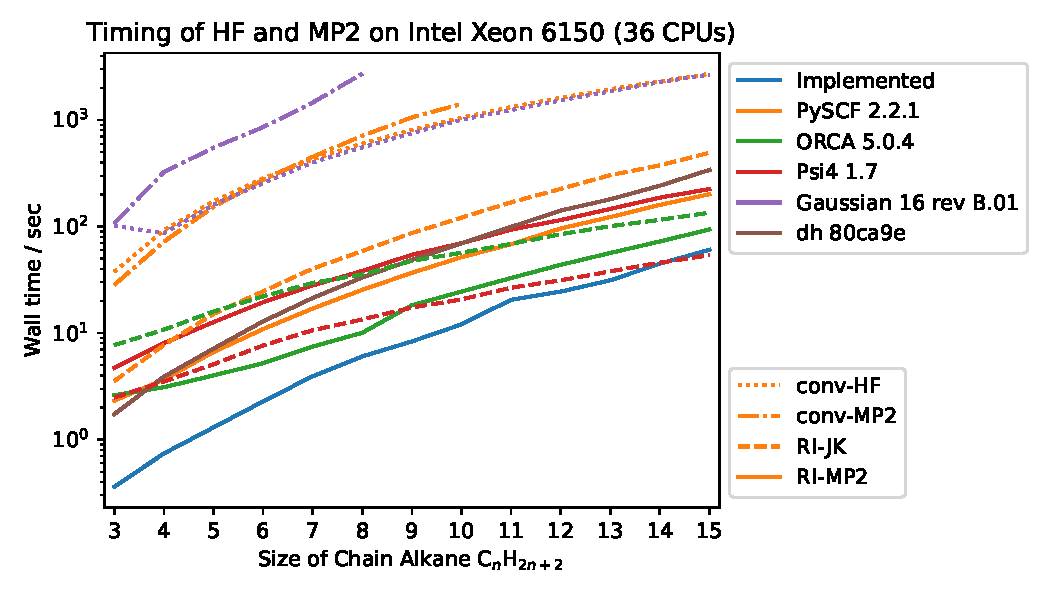
\includegraphics[width=0.8\textwidth]{assets/timing-rimp2-implemented.pdf}

  \raggedright
  \begin{itemize}[nosep]
    \item 测评体系是链状烷烃 \ce{C_n H_{2n+2}},基组 def2-QZVPPD、RI-JK 与 RI-MP2 分别使用对应于 def2-QZVPPD 的辅助基组。计算设备为 Intel Xeon Gold 6150 (36 cores, 72 threads, 2 NUMA nodes);所有计算任务使用 36 线程 (PySCF, Psi4, Gaussian) 或进程 (ORCA) 并行。
    \item 图中 Implemented (蓝色线) 是通过与附录 \ref{sec.python-ri-mp2} 相似的纯 Python 程序的测评结果。
    \item 除 PySCF conv-HF 或 conv-MP2 限制使用 32 GB 内存空间外,其余情形提供 300 GB 的充足内存以保证所有 3c-2e 积分可置于内存中,并使用默认的算法进行计算。
    \item 不同程序的自洽场收敛判据不同、迭代步数不同。3 碳以上所有测评涉及程序的迭代步数一般在 9--11 步。
  \end{itemize}
\end{figure}

\subsubsection{偶极矩与静态极化率:偶极电场下的能量与梯度}

这一小节将引入偶极电场下的梯度量:偶极矩 (dipole) 与静态极化率 (static polarizability)\footnote{需要指出,极化率作为二阶梯度量,与 M\o{}ller-Plesset 二阶微扰 (MP2) 一样,可以通过 Rayleigh-Schr\"odinger 微扰理论导出。在该理论下,还可以得出一定频率下外加偶极电场扰动下能量的变化;此情形下的极化率称为动态极化率 (dynamic polarizability)。动态极化率在以化学增强 SERS 为代表的问题中有重要的意义\cite{Jensen-Schatz.CSR.2008, Perez-Jimenez-Ren.CS.2020, Li-Xu.C.2022};但在本工作中,我们将不考察动态极化率问题。}。

在偶极电场 $\pmb{\mathcal{E}}$ 的微扰下,Hamilton 算符的形式\alert{在绪论中}已经阐明。令外场下微扰 Hamilton 算符为 $\hat H^{(1)}$;微扰算符是由单电子算符与常数项所构成:
\begin{equation}
  \label{eq.electric-perturbed-hamiltonian}
  \hat H^{(1)} = - \sum_i^{n_\mathrm{elec}} \pmb{\mathcal{E}}^\dagger \bm{r}_i + \sum_{A}^{n_\mathrm{atom}} Z_A \pmb{\mathcal{E}}^\dagger \bm{A} \quad \text{(not Einstein notation)}
\end{equation}
作为三维向量的偶极矩 $\bm{\mu}$ 与作为三维矩阵的极化率 $\bm{\alpha}$ 分别定义为分子基态能量受偶极电场扰动的一阶导数与二阶导数量\cite{Atkins-Friedman.Oxford.2011}:
\begin{align}
  E(\pmb{\mathcal{E}}) &= E(\bm{0}) + \pmb{\mathcal{E}}^\dagger \cdot \bm{\mu} - \pmb{\mathcal{E}} \cdot \bm{\alpha} \cdot \pmb{\mathcal{E}} + o(|\pmb{\mathcal{E}}|^3) \notag\\
  &= E(\bm{0}) + \mathcal{E}_t \mu_t - \mathcal{E}_t \alpha_{ts} \mathcal{E}_s + o(|\pmb{\mathcal{E}}|^3)
\end{align}
上式的 $t, s$ 指代坐标分量 $x, y, z$。偶极矩 $\bm{\mu}$ 与极化率 $\bm{\alpha}$ 也可以通过下式定义:
\begin{equation}
  \bm{\mu} := \left. \frac{\mathrm{d} E}{\mathrm{d} \pmb{\mathcal{E}}} \right|_{\pmb{\mathcal{E}} = \bm{0}}, \quad
  \bm{\alpha} := - \left. \frac{\mathrm{d}^2 E}{\mathrm{d} \pmb{\mathcal{E}}^2} \right|_{\pmb{\mathcal{E}} = \bm{0}}
\end{equation}
分量的数值定义为
\begin{equation}
  \mu_t = \left. \frac{\mathrm{d} E}{\mathrm{d} \mathcal{E}_t} \right|_{\pmb{\mathcal{E}} = \bm{0}}, \quad
  \alpha_{ts} = - \left. \frac{\mathrm{d}^2 E}{\mathrm{d} \mathcal{E}_t \mathrm{d} \mathcal{E}_s} \right|_{\pmb{\mathcal{E}} = \bm{0}}
\end{equation}

在计算化学程序中,定义微扰下的单电子积分
\begin{align}
  h_{\mu \nu}^{t} &= - \int \phi_\mu (\bm{r}) t \phi_\nu (\bm{r}) \, \mathrm{d} \bm{r} \\
  \label{eq.def.huv-with-perturb}
  h_{\mu \nu} (\pmb{\mathcal{E}}) &= h_{\mu \nu} (\bm{0}) + \mathcal{E}_t h_{\mu \nu}^t
\end{align}
以及微扰下的原子核能量
\begin{equation}
  E^\textsf{non-elec} (\pmb{\mathcal{E}}) = \frac{1}{2} \frac{Z_A Z_B}{r_{AB}} + Z_A \mathcal{E}_t A_t
\end{equation}
可以求得偶极电场 $\pmb{\mathcal{E}}$ 下的分子能量。因此,偶极矩 $\bm{\mu}$ 与极化率 $\bm{\alpha}$ 可以通过对 $E^\textsf{tot} (\pmb{\mathcal{E}})$ 作数值差分或解析导数得到。

\begin{figure}
  \centering
  \caption{能量在外场下的变化情况 $E(\pmb{\mathcal{E}})$。图中的体系是键长 0.9914 \AA、键角 116.10$^\circ$ 的 \ce{NH_3} 体系;$C_3$ 旋转轴与 $z$ 轴重合;计算模型为 HF/6-31G;外场沿 $z$ 轴即外场强度向量 $\pmb{\mathcal{E}}^\dagger = (0, 0, \mathcal{E}_z)$。蓝色曲线绘制了 $E(\pmb{\mathcal{E}})$ 关于 $\mathcal{E}_z$ 的函数。橙色曲线绘制了 $\mathcal{E}_z = 0$ 时 $\partial_{\mathcal{E}_z} E$ 的导数值;该导数值等于偶极矩在 $z$ 轴上的分量 $\mu_z$。}
  \label{fig.NumDipole-z}
  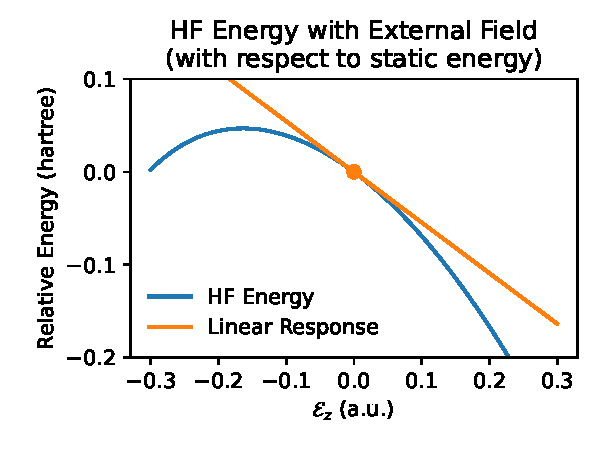
\includegraphics[width=0.5\textwidth]{assets/NumDipole-z.pdf}
\end{figure}

需要指出,式 (\ref{eq.electric-perturbed-hamiltonian}) 所述的 $- \pmb{\mathcal{E}}^\dagger \bm{r}$ 形式的偶极电场仅仅是外加电场其中一种可能性。若外加电场是 $- \pmb{\mathcal{E}}^\dagger \bm{Q} \pmb{\mathcal{E}}$ 的形式,其中
\begin{equation*}
  \bm{Q} =
  \begin{pmatrix}
    x^2 & xy & xz \\
    yx & y^2 & yz \\
    zx & zy & z^2
  \end{pmatrix}
\end{equation*}
那么在该类型的外加电场下,一阶梯度将给出四极矩 (quadrupole)。电场的其它多级展开还将给出八极矩 (octupole)、十六极矩 (hexadecapole) 等等。所有类型的外加电场,在计算化学程序中都表现为对单电子积分与原子核能量的微扰,而对双电子积分、DFA 格点积分能量、原子轨道等部分不产生微扰。本工作着重于极化率,即 $- \pmb{\mathcal{E}}^\dagger \bm{r}$ 形式的偶极电场下的一阶与二阶梯度,即偶极矩与静态极化率的推导与程序实现;但该推导能比较容易地拓展到其它形式的外加电场一阶与二阶梯度。

\subsection{双杂化泛函电性质解析梯度}
\label{sec.3.theory}

本节将在 xDH 框架下,讨论电性质导数问题;被求导的性质将以 $\mathbb{A}, \mathbb{B}$ 表示。除非特别指明,一般讨论的是闭壳层情形。不同于分子坐标导数或 GIAO 轨道导数,许多 Skeleton 导数对于电性质是零值;因此,这里的讨论不适合推广到所有的梯度问题中。

\subsubsection{正交条件、自洽场条件与自洽场泛函对密度矩阵的依赖关系}

在开始梯度理论推演前,先对式 (\ref{eq.def.eng-SCF}) 所给出的自洽场计算过程与结果作必要的回顾。这一小节不考虑外场效应。

作为低阶泛函,闭壳层自洽场能量 $E^\textsf{SCF}$ 仅决定于依式 (\ref{eq.def.dm-scf-closed}) 所定义的双占据的密度矩阵 $D_{\mu \nu}$。密度矩阵 $D_{\mu \nu}$ 由分子轨道系数 $C_{\mu i}$ 构成;分子轨道正交归一条件 (后文简称为\textsf{正交条件}) 具体表达为
\begin{empheq}[box=\fbox]{equation}
  \label{eq.constraint.ortho}
  S_{pq} = C_{\mu p} S_{\mu \nu} C_{\nu q} = \delta_{pq} \quad \text{(orthogonalization constraint)}
\end{empheq}
原子轨道基的 Fock 矩阵定义为自洽场能量对密度矩阵的导数:
\begin{equation}
  \label{eq.def.fock-ao}
  F_{\mu \nu} := \frac{\partial E^\textsf{SCF}}{\partial D_{\mu \nu}}
\end{equation}
它是自洽场作为变分方法的重要中间量,且为对称矩阵。自洽场能量 $E^\textsf{SCF}$ 对占据轨道 $C_{\mu i}$ 的导数为
\begin{align}
  \label{eq.eng-deriv-wrt-coeff}
  \frac{\partial E^\textsf{SCF}}{\partial C_{\mu i}} &= \frac{\partial E^\textsf{SCF}}{\partial D_{\kappa \lambda}} \frac{\partial D_{\kappa \lambda}}{\partial C_{\mu i}}
  = F_{\kappa \lambda} \left( 2 \delta_{\kappa \mu} C_{\lambda i} + 2 \delta_{\lambda \mu} C_{\kappa i} \right) = 4 F_{\mu \nu} C_{\nu i}
\end{align}
占据轨道系数 $C_{\mu i}$ 是通过引入正交条件 (\ref{eq.constraint.ortho}) 对 $E^\textsf{SCF}$ 作条件极小值计算得到。定义对称的 Lagrange 乘子矩阵为 $\varepsilon_{jk}$;下式作为变分方程,对指标 $\nu, j, k$ 求和:
\begin{equation}
  \label{eq.hartree-fock-roothaan}
  \frac{\partial}{\partial C_{\mu i}} \big( E^\textsf{SCF} - 2 \varepsilon_{jk} (S_{jk} - \delta_{jk}) \big) = 4 \big( F_{\mu \nu} C_{\nu i} - S_{\mu \nu} C_{\nu j} \varepsilon_{ji} \big) = 0
\end{equation}
若自洽场泛函是 Hartree-Fock,那么上式即 Hartree-Fock-Roothaan 方程\cite{Roothaan-Roothaan.RMP.1951}。

$F_{\mu \nu}$ 作为原子轨道基下的矩阵,秩 $n_\mathrm{MO}$ 明显大于占据轨道数 $n_\mathrm{nocc}$;在程序实现中,一般将求取 $n_\mathrm{MO}$ 个分子轨道的系数 $C_{\mu p}$:
\begin{equation}
  \label{eq.SCF-working-equation}
  F_{\mu \nu} C_{\nu p} = S_{\mu \nu} C_{\nu q} \varepsilon_{qp} \quad \text{(SCF working equation)}
\end{equation}
但需要注意到,只有占据轨道对自洽场能量产生贡献。关于自洽场对占据布局的限制条件,可以通过对式 (\ref{eq.hartree-fock-roothaan}) 等式两边乘以非占轨道系数 $C_{\mu a}$、并对原子轨道指标 $\mu, \nu$ 求和结果所体现:
\begin{equation*}
  4 (C_{\mu a} F_{\mu \nu} C_{\nu i} - C_{\mu a} S_{\mu \nu} C_{\nu j} \varepsilon_{ji}) = 4 (F_{ai} - S_{aj} \varepsilon_{ji}) = 0
\end{equation*}
或更简洁地,Fock 矩阵在分子轨道基下是分块对角化的:
\begin{empheq}[box=\fbox]{equation}
  \label{eq.constraint.SCF}
  F_{ai} = 0 \quad \text{(SCF constraint)}
\end{empheq}
上式在后文称为\textsf{自洽场条件};推演过程利用了正交条件 (\ref{eq.constraint.ortho}) 所给出的 $S_{aj} = 0$ (占据轨道与非占轨道角标不可能一致)。

正交条件与自洽场条件是梯度推演中,所有必要的额外限制条件。

最后,为了后面推导的便利,这里引入 A 张量的前导张量 $\tilde A_{\mu \nu, \kappa \lambda}$ (Fock 轨道响应张量) 作为 Fock 矩阵对密度矩阵的导数量:
\begin{equation}
  \label{eq.def.Auvkl-pre}
  \tilde A_{\mu \nu, \kappa \lambda} := \frac{\partial^2 E^\textsf{SCF}}{\partial D_{\mu \nu} \partial D_{\kappa \lambda}} = \frac{\partial F_{\mu \nu}}{\partial D_{\kappa \lambda}}
\end{equation}
该张量通常具有 4 重对称性:
\begin{equation*}
  \tilde A_{\mu \nu, \kappa \lambda} = \tilde A_{\kappa \lambda, \mu \nu} = \tilde A_{\nu \mu, \lambda \kappa} = \tilde A_{\lambda \kappa, \nu \mu}
\end{equation*}
但需要指出,若交换能 $E_\mathrm{x}^\textsf{exact}$ (或其长程的对应 $E_\mathrm{x}^\textsf{LR}$) 对能量项有贡献,那么该张量不是 8 重对称性的 (即不满足 $\tilde A_{\mu \nu, \kappa \lambda} = \tilde A_{\mu \nu, \lambda \kappa}$)。出于便利,我们将定义下述 8 重对称性的张量 $A_{\mu \nu, \kappa \lambda}$,该张量称为 A 张量:
\begin{equation}
  \label{eq.def.Auvkl}
  A_{\mu \nu, \kappa \lambda} := 2 \left( \tilde A_{\mu \nu, \kappa \lambda} + \tilde A_{\mu \nu, \lambda \kappa} \right)
\end{equation}
上式定义中的 2 倍,是出于闭壳层情形下,下述表达式方便而给出:
\begin{align}
  \frac{\partial F_{\mu \nu}}{\partial C_{\kappa i}} &= \frac{\partial F_{\mu \nu}}{\partial D_{\eta \lambda}} \frac{\partial D_{\eta \lambda}}{\partial C_{\kappa i}}
  = 2 \tilde A_{\mu \nu, \eta \kappa} \left( \delta_{\eta \kappa} C_{\lambda i} + \delta_{\lambda \kappa} C_{\eta i} \right) \notag\\
  &= 2 \left( \tilde A_{\mu \nu, \kappa \lambda} + \tilde A_{\mu \nu, \lambda \kappa} \right) C_{\lambda i} \notag\\
  &= A_{\mu \nu, \kappa \lambda} C_{\lambda i} = A_{\mu \nu, \kappa i}
\end{align}
上式的第三个等号利用了被求和角标 $\eta, \lambda$ 的轮换。

\subsubsection{一阶梯度:轨道系数随外场的变化}

自洽场泛函 $E^\textsf{SCF}$ 与能量泛函 $E^\textsf{xDH}$ 的运算共用同一轨道系数 $C_{\mu i}$。这一小节进一步讨论正交条件、自洽场条件在外场微扰 $\mathbb{A}$ 下的响应,并籍此给出描述轨道系数在外场微扰下变化的 U 矩阵 $U_{pq}^\mathbb{A}$\footnote{式 (\ref{eq.def.U}) 中 U 矩阵的定义并非在等式左边。利用正交条件 (\ref{eq.constraint.ortho}),可知
\begin{equation*}
  U_{pq}^\mathbb{A} := C_{\mu p} S_{\mu \nu} \partial_\mathbb{A} C_{\nu q}
\end{equation*}
该式与定义式 (\ref{eq.def.U}) 是等价的。出于推演方便,我们仅使用定义式 (\ref{eq.def.U})。}:
\begin{empheq}[box=\fbox]{equation}
  \label{eq.def.U}
  \partial_\mathbb{A} C_{\mu q} = C_{\mu p} U_{pq}^\mathbb{A}
\end{empheq}
这一小节首先确定 U 矩阵在占据-非占部分 $U_{ai}^\mathbb{A}$ 的表达式。其余部分在后一小节详细描述。

对正交条件 (\ref{eq.constraint.ortho}) 作性质 $\mathbb{A}$ 的导数:
\begin{align*}
  \partial_{\mathbb{A}} S_{pq} &= \partial_\mathbb{A} C_{\mu p} S_{\mu \nu} C_{\nu q} + C_{\mu p} \partial_\mathbb{A} S_{\mu \nu} C_{\nu q} + C_{\mu p} S_{\mu \nu} \partial_\mathbb{A} C_{\nu q} \notag\\
  &= S_{mq} U_{mp}^\mathbb{A} + S_{pm} U_{mq}^\mathbb{A} = U_{pq}^\mathbb{A} + U_{qp}^\mathbb{A} = 0
\end{align*}
或更简洁地,
\begin{empheq}[box=\fbox]{equation}
  \label{eq.collary.ortho}
  U_{pq}^\mathbb{A} + U_{qp}^\mathbb{A} = 0 \quad \text{(corollary of orthogonalization constraint)}
\end{empheq}
其中,$\partial_\mathbb{A} S_{pq}$ 推导过程中利用到电性质微扰下基轨道没有变化,因此 $\partial_\mathbb{A} S_{\mu \nu} = 0$。上述结论表明,U 矩阵在电性质导数下是反对称的\footnote{需要指出,对于其它性质梯度,由于 $\partial_\mathbb{A} S_{\mu \nu}$ 未必是零,因此 U 矩阵一般来说未必是反对称或反厄米的。后文将有许多结论只能用于电性质微扰,而无法简单地扩展到所有情形。在本工作中,不会一一列举所有情形。}。

进而将对自洽场条件 (\ref{eq.constraint.SCF}) 的等式两边作性质 $\mathbb{A}$ 的导数。但在考虑 $\partial_\mathbb{A} F_{ai}$ 前,我们先考虑更一般的原子轨道基下 Fock 矩阵的导数:
\begin{equation}
  \label{eq.deduct.pd-Fuv}
  \partial_\mathbb{A} F_{\mu \nu} = \partial_\mathbb{A}^\mathrm{S} F_{\mu \nu} + \partial_\mathbb{A}^\mathrm{U} F_{\mu \nu}
  = F_{\mu \nu}^\mathbb{A} + \frac{\partial F_{\mu \nu}}{\partial C_{\kappa i}} \partial_\mathbb{A} C_{\kappa i}= F_{\mu \nu}^\mathbb{A} + A_{\mu \nu, mi} U_{mi}^\mathbb{A}
\end{equation}
其中,$F_{\mu \nu}^\mathbb{A} := \partial_\mathbb{A}^\mathrm{S} F_{\mu \nu}$ 定义为不受密度矩阵扰动、而仅受外场扰动产生变化的 Skeleton 导数部分。作为特例,对于外加偶极电场而言,从式 (\ref{eq.def.huv-with-perturb}) 附近的讨论出发,仅有单电子算符部分产生贡献:
\begin{align}
  \label{eq.def.sleketon-huv}
  F_{\mu \nu}^{\mathcal{E}_t} = h_{\mu \nu}^{\mathcal{E}_t} &:= \partial_{\mathcal{E}_t} h_{\mu \nu} = h_{\mu \nu}^t \\
  F_{pq}^{\mathcal{E}_t} = h_{pq}^{\mathcal{E}_t} &:= C_{\mu p} F_{\mu \nu}^{\mathcal{E}_t} C_{\nu q}
\end{align}
对于多级展开的外电场也是类似的;我们将在所有电性质导数问题中,假定 $F_{\mu \nu}^\mathbb{A} = h_{\mu \nu}^\mathbb{A}$ 与 $F_{pq}^\mathbb{A} = h_{pq}^\mathbb{A}$。

在得到原子轨道基 Fock 矩阵导数 $\partial_\mathbb{A} F_{\mu \nu}$ 后,分子轨道下的导数可以顺势得到:
\begin{align}
  \label{eq.pd-Fpq-0}
  \partial_\mathbb{A} F_{pq} &= F_{mq} U_{mp}^\mathbb{A} + F_{pm} U_{mq}^\mathbb{A} + C_{\mu p} \partial_\mathbb{A} F_{\mu \nu} C_{\nu q} \notag\\
  &= F_{mq} U_{mp}^\mathbb{A} + F_{pm} U_{mq}^\mathbb{A} + F_{pq}^\mathbb{A} + A_{pq, mj} U_{mj}^\mathbb{A}
\end{align}
上式在二阶梯度求取、以及 MP2 的激发张量导数计算上经常用到;但在这一小节,我们只对其非占-占据部分感兴趣。对自洽场条件 (\ref{eq.constraint.SCF}) 的两边求导,得到
\begin{align}
  \label{eq.pd-Fai-0}
  \partial_\mathbb{A} F_{ai} &= F_{mi} U_{ma}^\mathbb{A} + F_{am} U_{mi}^\mathbb{A} + F_{ai}^\mathbb{A} + A_{ai, mj} U_{mj}^\mathbb{A} = 0
  \quad \text{(corollary of SCF constraint)}
\end{align}
若引入\textsf{正则自洽场条件},即 Fock 矩阵是对角化的:
\begin{equation}
  \label{eq.constraint.canonical-SCF}
  F_{pq} = \varepsilon_p \delta_{pq} \quad \text{(canonical SCF constraint)}
\end{equation}
那么,式 (\ref{eq.pd-Fai-0}) 可以写为
\begin{equation}
  \label{eq.intermediate-pd-Fai-1}
  \partial_\mathbb{A} F_{ai} = \varepsilon_i U_{ia}^\mathbb{A} + \varepsilon_a U_{ai}^\mathbb{A} + F_{ai}^\mathbb{A} + A_{ai, mj} U_{mj}^\mathbb{A} = 0
\end{equation}
该式还可以简化。利用 U 矩阵的反对称性和 A 张量的对称性,$A_{ai, mj} U_{mj}^\mathbb{A}$ 中 $m$ 仅对占据轨道求和时,
\begin{align*}
  \partial_\mathbb{A} F_{ai} \leftarrow A_{ai, kj} U_{kj}^\mathbb{A} = \frac{1}{2} \left( A_{ai, kj} U_{kj}^\mathbb{A} + A_{ai, jk} U_{kj}^\mathbb{A} \right) = \frac{1}{2} \left( A_{ai, kj} U_{kj}^\mathbb{A} + A_{ai, kj} U_{jk}^\mathbb{A} \right) = 0
\end{align*}
上式的 $\leftarrow$ 是指右侧表达式对左侧表达式产生贡献。因此,式 (\ref{eq.intermediate-pd-Fai-1}) 的 $A_{ai, mj} U_{mj}^\mathbb{A}$ 中 $m$ 仅有非占轨道求和的贡献。从而,式 (\ref{eq.intermediate-pd-Fai-1}) 简化为
\begin{empheq}[box=\fbox]{align}
  \label{eq.CP-SCF}
  F_{ai}^\mathbb{A} &= - (\varepsilon_a - \varepsilon_i) U_{ai}^\mathbb{A} - A_{ai, bj} U_{bj}^\mathbb{A} \notag\\
  &= - \left( (\varepsilon_a - \varepsilon_i) \delta_{ai, bj} + A_{ai, bj} \right) U_{bj}^\mathbb{A} \quad \text{(CP-SCF)}
\end{empheq}
该式是电性质导数下的 CP-SCF (\underline{C}oupled-\underline{P}erturbed \underline{SCF}) 方程;通过该方程可以求得 U 矩阵的非占-占据部分 $U_{ai}^\mathbb{A}$。其耦合微扰的意义是,不仅 Hamilton 算符受外场扰动、自洽场波函数也因 Hamilton 算符的微扰而随之产生变化;CP-SCF 方程所给出的 U 矩阵确定了轨道系数 (作为描述自洽场波函数的参数) 是如何随外场发生扰动的。

\subsubsection{一阶梯度:U 矩阵占据-占据和非占-非占部分}
\label{sec.3.Uia-Uai}

对于自洽场方法,轨道正交条件 $S_{pq} = 0$ 与自洽场条件 $F_{ai} = 0$ 是必须满足的条件;但正则自洽场条件 $F_{pq} = \varepsilon_p \delta_{pq}$ 仅仅是出于公式推导的便利与程序实现的方便,而引入的可选条件。这意味着在微扰下,只有占据与非占轨道相互之间的变化情况是非平凡的,即 $U_{ai}^\mathbb{A}$ 与 $U_{ia}^\mathbb{A} = - U_{ai}^\mathbb{A}$ 的数值是非平凡的;占据-占据的 $U_{ij}^\mathbb{A}$ 与非占-非占的 $U_{ab}^\mathbb{A}$ 的数值并非是关键的。因此,只要 $U_{ij}^\mathbb{A}$ 与 $U_{ab}^\mathbb{A}$ 满足式 (\ref{eq.collary.ortho}) 给出的轨道正交条件的结论即可。对于电性质导数而言,最简单的定义方式是置零:
\begin{empheq}[box=\fbox]{equation}
  \label{eq.Uij-Uab-zero}
  U_{ij}^\mathbb{A} = U_{ab}^\mathbb{A} = 0 \quad \text{(definition of program implementation)}
\end{empheq}

在程序实现中,我们将依照式 (\ref{eq.Uij-Uab-zero}) 所给出的定义实现 U 矩阵的占据-占据与非占-非占部分。该式将使得 Fock 矩阵的导数在非对角元上未必为零:
\begin{equation}
  \label{eq.pd-Fpq-not-diagonal}
  \partial_\mathbb{A} F_{pq} \not \equiv 0 \quad (p \neq q, \text{(\ref{eq.Uij-Uab-zero}) satisfied})
\end{equation}
这意味着,Fock 矩阵在外场为零的情形下仍然可以是对角化的,即满足 $F_{pq} |_{\mathbb{A} = 0} = \varepsilon_p \delta_{pq}$;但外场不为零时,Fock 矩阵不再是对角化的;这不同于正交条件与自洽场条件\footnote{许多微扰能形式,譬如 MP2、IEPA、MP2/cr、RPA,在计算时需要引入自洽场轨道能 $\varepsilon_p$;但若 Fock 矩阵 $F_{pq}$ 并非对角的,那么轨道能就无法准确地定义。如果某一方法可以由 Fock 矩阵定义,且无论 Fock 矩阵是否对角、能量结果都是一致的,那么该方法一般来说是正交变换不变的 (Unitary Invariance)。MP2、RPA 方法是正交不变的,但 IEPA、MP2/cr 方法则并非正交不变。这一小节涉及到的推演,特别是式 (\ref{eq.Uij-Uab-zero}) 的定义,应仅对正交不变方法是合理的。}。

下面我们将讨论式 (\ref{eq.pd-Fpq-not-diagonal}) 占据-占据部分情形。利用 Fock 矩阵为对角阵、以及 U 矩阵反对称性质,
\begin{align}
  \partial_\mathbb{A} F_{ij} &= F_{im} U_{mj}^\mathbb{A} + F_{mj} U_{mi}^\mathbb{A} + F_{ij}^\mathbb{A} + A_{ij, mk} U_{mk}^\mathbb{A} \notag\\
  &= (\varepsilon_i - \varepsilon_j) U_{ij}^\mathbb{A} + F_{ij}^\mathbb{A} + A_{ij, bk} U_{bk}^\mathbb{A}
\end{align}
在上式的推导中,当角标 $m$ 作为占据轨道 $l$ 时,贡献项 $\partial_\mathbb{A} F_{ij} \leftarrow A_{ij, lk} U_{lk}^\mathbb{A}$ 由于 $A_{ij, lk}$ 与 $U_{lk}^\mathbb{A}$ 关于 $l, k$ 角标分别对称与反对称,因此该项为零。故而,仅有角标 $m$ 取非占轨道 $b$ 时,$\partial_\mathbb{A} F_{ij} \leftarrow A_{ij, bk} U_{bk}^\mathbb{A}$ 是非平凡的贡献项。通过 CP-SCF 方程,我们已经可以求得 $U_{bj}^\mathbb{A}$;从而,通过上式可以求得
\begin{equation}
  U_{ij}^\mathbb{A} = 
  \begin{cases}
    \displaystyle
    - \frac{F_{ij}^\mathbb{A} + A_{ij, bk} U_{bk}^\mathbb{A} - \partial_\mathbb{A} F_{ij}}{\varepsilon_i - \varepsilon_j} & (i \neq j) \\
    0 & (i = j)
  \end{cases}
\end{equation}
其中,$U_{ii}^\mathbb{A} = 0$ 直接由轨道正交条件 (\ref{eq.collary.ortho}) 所导出。

假使,Fock 矩阵导数也满足正则自洽场条件,即 $\partial_\mathbb{A} F_{ij} = \delta_{ij} \partial_\mathbb{A} \varepsilon_i$,那么
\begin{equation}
  \label{eq.unstable-Uij}
  U_{ij}^\mathbb{A} = - \frac{F_{ij}^\mathbb{A} + A_{ij, bk} U_{bk}^\mathbb{A}}{\varepsilon_i - \varepsilon_j} \quad \left( i \neq j, \, \partial_\mathbb{A} F_{ij} = 0 \right)
\end{equation}
上式的分子一般非零,而分母 $\varepsilon_i - \varepsilon_j$ 则有可能接近于零;举例而言,甲烷分子的最高能级占据轨道为 $T_d$ 不可约表示,即三重简并,因此存在 $i \neq j$ 且 $\varepsilon_i - \varepsilon_j = 0$ 的情形,从而将 $U_{ij}^\mathbb{A}$ 推向无穷大,导致严重的数值误差。因此,为在程序实现中避免这类数值误差,那么 $\partial_\mathbb{A} F_{ij}$ 不适合在 $i \neq j$ 时设为零。

方才分析的是 Fock 矩阵导数占据-占据部分 $\partial_\mathbb{A} F_{ij}$;对于非占-非占部分 $\partial_\mathbb{A} F_{ab}$ 也有类似的结论。

需要指出,尽管令 $\partial_\mathbb{A} F_{pq}$ 为非对角矩阵尽管可以避免数值误差,但同时也有可能增加计算量。对于后续将定义的 MP2 型相关激发张量 $t_{ij}^{ab}$ 的导数,
\begin{equation*}
  \partial_\mathbb{A} t_{ij}^{ab} \leftarrow - \partial_\mathbb{A} F_{ca} t_{ij}^{cb}
\end{equation*}
若 $\partial_\mathbb{A} F_{ca}$ 不是对角矩阵,那么上述贡献项的计算复杂度将是 $O(n_\mathrm{prop} n_\mathrm{occ}^2 n_\mathrm{vir}^3)$,即随体系增大而呈五次复杂度 (作为电性质,偶极外场的 $n_\mathrm{prop} = 3$ 即三个坐标分量方向);但若 $\partial_\mathbb{A} F_{ca}$ 是对角矩阵,则尽管有更低的 $O(n_\mathrm{prop} n_\mathrm{occ}^2 n_\mathrm{vir}^2)$ 即四次复杂度,但仍然是内存密集型运算且存在潜在严重数值误差的可能性。一种可能的解决方案是,对于简并或近简并的一部分轨道,定义非对角的 $\partial_\mathbb{A} F_{pq}$;而剩余下来不存在简并情况的轨道,它们构成的 $\partial_\mathbb{A} F_{pq}$ 仍然是对角的。在这种方案下由于三维空间的最大不可约表示是三维,因此 FLOPs 不会超过 9 倍于 $n_\mathrm{prop} n_\mathrm{occ}^2 n_\mathrm{vir}^2$ 的乘积累加运算\cite{Stoychev-Neese.JCTC.2018}。但这种方案并非简单的张量乘积,程序实现上会引入一定的复杂性;在我们目前的程序实现中,没有将其纳入考虑。

\subsubsection{一阶梯度:能量泛函导数}

这一小节讨论能量泛函 $E^\textsf{xDH}$ 在性质 $\mathbb{A}$ 微扰下的导数。

xDH 总能量的全导数可以分为 Skeleton 部分与对轨道系数的导数两部分:
\begin{equation}
  \label{eq.def.pdA-xDH-0}
  \partial_\mathbb{A} E^\textsf{xDH} = \partial_\mathbb{A}^\mathrm{S} E^\textsf{xDH} + \frac{\partial E^\textsf{xDH}}{\partial C_{\mu q}} \partial_\mathbb{A} C_{\mu q}
\end{equation}
对于轨道系数导数部分,我们作更多讨论。定义 xDH 的广义 Fock 矩阵 (generalized Fock matrix) 为
\begin{equation}
  \label{eq.def.generalized-fock}
  F_{pq}^\textsf{xDH} := C_{\mu p} \frac{\partial E^\textsf{xDH}}{\partial C_{\mu q}}
\end{equation}
该矩阵的性质是
\begin{itemize}[nosep]
  \item 若 $E^\textsf{xDH} = E^\textsf{SCF}$,则广义 Fock 矩阵的占据-占据部分 $F_{ij}^\textsf{xDH}$ 退化到自洽场 Fock 矩阵 $F_{ij}$;但非占-非占部分 $F_{ab}^\textsf{xDH}$ 数值上是零,因非占轨道对自洽场能量没有影响;
  \item 广义 Fock 矩阵不一定是对角化的、对称的;非占-占据或占据-非占部分也未必为零\footnote{对于一般的 bDH 或 xDH 型泛函,广义 Fock 矩阵不一定对角化。轨道优化 (orbital-optimized) MP2 或双杂化泛函,则要求广义 Fock 矩阵对角化是对角化的\cite{Bozkaya-Sherrill.JCP.2011}。但轨道优化的代价,是要多次迭代地计算广义 Fock 矩阵、单步 MP2 相关能因非正则 SCF 的缘故需迭代计算得到,且广义 Fock 矩阵计算消耗一般不小于 MP2 相关能计算。}。
\end{itemize}
进而引入 xDH Lagrangian 为广义 Fock 反对称化矩阵\footnote{在本文中,Lagrangian 通过广义 Fock 矩阵所定义。但一般来说,Lagrangian 应当通过轨道或密度在旋转矩阵下的导数定义\cite{Helgaker-Jorgensen.Wiley.2013};因此,应当认为广义 Fock 反对称化矩阵的结果等于 Lagrangian,而非后者为前者所定义。但比较严格地引入 Lagrangian 将占用一定的篇幅。}:
\begin{equation}
  \label{eq.def.lagrangian}
  L_{pq}^\textsf{xDH} := F_{pq}^\textsf{xDH} - F_{qp}^\textsf{xDH}
\end{equation}
注意到对于电性质而言,U 矩阵是反对称、且在占据-占据部分与非占-非占部分可以置零;因此,
\begin{align}
  \label{eq.derivation-contrib-Lai-to-engderiv}
  \partial_\mathbb{A} E^\textsf{xDH} &\leftarrow \frac{\partial E^\textsf{xDH}}{\partial C_{\mu q}} \frac{\partial C_{\mu q}}{\partial \mathbb{A}} = F_{pq}^\textsf{xDH} U_{pq}^\mathbb{A} \notag\\
  &= F_{ai}^\textsf{xDH} U_{ai}^\mathbb{A} + F_{ia}^\textsf{xDH} U_{ia}^\mathbb{A} + F_{ij}^\textsf{xDH} U_{ij}^\mathbb{A} + F_{ab}^\textsf{xDH} U_{ab}^\mathbb{A} \notag\\
  &= (F_{ai}^\textsf{xDH} - F_{ia}^\textsf{xDH}) U_{ai}^\mathbb{A} + 0 = L_{ai}^\textsf{xDH} U_{ai}^\mathbb{A}
\end{align}
特别地,对于自洽场方法,$L_{ai}^\textsf{SCF} = 0$。从而,电性质微扰下 xDH 一阶泛函能量导数可以写为
\begin{empheq}[box=\fbox]{equation}
  \label{eq.derivation-xdh-energy-deriv-abstract}
  \partial_\mathbb{A} E^\textsf{xDH} = \partial_\mathbb{A}^\mathrm{S} E^\textsf{xDH} + L_{ai}^\textsf{xDH} U_{ai}^\mathbb{A}
\end{empheq}

正因为 xDH 型泛函包含了公式形式复杂的 $E^\textsf{PT} [\mathbf{C}]$、以及其 Lagrangian 一般地非零 $L_{ai}^\textsf{xDH} \not \equiv 0$,从而 xDH 型泛函的梯度理论相比之自洽场而言要复杂不少。

\subsubsection{一阶梯度:约化密度矩阵}

约化密度与电性质 Skeleton 导数有直接的联系。这里先以 CI 波函数 $| \Psi^\textsf{CI} \rangle$ 开始讨论,随后引申到 xDH 型泛函的约化密度。本小节与下一小节同时参考 Trucks 等的文献\cite{Trucks-Bartlett.CPL.1988}。

CI 的 (一阶) 约化密度 (RDM, \underline{R}educed \underline{D}ensity \underline{M}atrix) 在分子轨道基下,一般定义为
\begin{equation}
  \label{eq.def.rdm-ci}
  D_{qp}^{\textsf{CI},\textsf{RDM}} := \frac{\langle \Psi^\textsf{CI} | a_p^\dagger a_q | \Psi^\textsf{CI} \rangle}{\langle \Psi^\textsf{CI} | \Psi^\textsf{CI} \rangle}
\end{equation}
约化密度矩阵的意义是,对于任意的单电子算符 $\hat o = o_{pq} a_p^\dagger a_q$,其期望值总是可以写为约化密度矩阵 $D_{qp}^{\textsf{CI},\textsf{RDM}}$ 与算符矩阵表示 $o_{pq}$ 的乘积:
\begin{equation*}
  \langle \hat o \rangle = \frac{\langle \Psi^\textsf{CI} | \hat o | \Psi^\textsf{CI} \rangle}{\langle \Psi^\textsf{CI} | \Psi^\textsf{CI} \rangle} = o_{pq} D_{qp}^{\textsf{CI},\textsf{RDM}}
\end{equation*}
注意到 $(a_p^\dagger a_q)^\dagger = a_q^\dagger a_p$,因此 $D_{qp}^{\textsf{CI},\textsf{RDM}}$ 是复共轭的。由于本工作仅考虑实数范围内的问题,因此可以认为约化密度矩阵是对称的。

现在考虑 CI 波函数的电性质 Skeleton 导数问题。对于 Hamilton 算符 $\hat H$,电子所引起的能量效应中,电性质仅对单电子算符 $\hat h = \hat T + \hat V_\mathrm{ext}$ 中的外势 $\hat V_\mathrm{ext}$ 有微扰贡献:
\begin{equation}
  \partial_\mathbb{A}^\mathrm{S} \hat H = \partial_\mathbb{A}^\mathrm{S} \hat h + \partial_\mathbb{A} \hat V_\textsf{non-elec} = h_{pq}^\mathbb{A} a_p^\dagger a_q + \partial_\mathbb{A} \hat V_\textsf{non-elec}
\end{equation}
依 Hellmann-Feynman 定理,算符期望的 Skeleton 导数等于 Skeleton 导数下算符的期望:
\begin{equation}
  \partial_\mathbb{A}^\mathrm{S} E^\textsf{CI} = \partial_\mathbb{A}^\mathrm{S} \langle \hat H \rangle = \langle \partial_\mathbb{A}^\mathrm{S} \hat H \rangle = \langle \partial_\mathbb{A}^\mathrm{S} \hat h \rangle + \partial_\mathbb{A} E^\textsf{non-elec} = h_{pq}^\mathbb{A} D_{pq}^{\textsf{CI}, \textsf{RDM}} + \partial_\mathbb{A} E^\textsf{non-elec}
\end{equation}

但作为常见的 xDH 型泛函能量贡献项,MP2 相关能或其它形式的相关能,在定义约化密度的问题上存在一些困难。MP2 方法的波函数并非是对 $\hat H$ 变分极小的,因此 Hellmann-Feynman 定理失效,从而 MP2 方法的约化密度矩阵不能通过与 CI 相同的方式 (\ref{eq.def.rdm-ci}) 所定义\footnote{
  注意到 MP2 相关能可以通过 Hylleraas 泛函给出\cite{Hylleraas-Hylleraas.ZP.1930, Pulay-Saeboe.TCA.1986}:
  \begin{equation*}
    E_\mathrm{c}^\textsf{(2)} = \min_{\Psi^{(1)}} \left( 2 \langle \Psi^\textsf{(1)} | \hat H - E^\textsf{0} | \Phi^\textsf{0} \rangle - \langle \Psi^\textsf{(1)} | \hat F - E^\textsf{0} | \Psi^\textsf{(1)} \rangle \right)
  \end{equation*}
  这里的 $\Phi^\textsf{0}$ 是 Hartree-Fock 行列式,$E^\textsf{0} = \langle \Phi^\textsf{0} | \hat F | \Phi^\textsf{0} \rangle$ 为零阶能量 (占据轨道能之和),$\Psi^\textsf{(1)}$ 是 MP2 相关波函数。上式可以看作对 $\Psi^\textsf{(1)}$ 取变分极小,因此 Hellmann-Feynman 定理适用于此。又由于 Brillouin 定理,$\Psi^\textsf{(1)}$ 只有二次激发项贡献、没有单次激发项,故对于任何单电子算符 $\hat o$ 总有 $\langle \Psi^\textsf{(1)} | \hat o | \Phi^\textsf{0} \rangle = 0$。故 MP2 相关部分对约化密度矩阵贡献是
  \begin{equation*}
    D_{pq}^{\textsf{(2)},\textsf{RDM}} = - \langle \Psi^\textsf{(1)} | a_p^\dagger a_q | \Psi^\textsf{(1)} \rangle
  \end{equation*}
  上述推导是基于自旋轨道下的;应当可以验证,在开壳层或闭壳层的限制下,通过 $\partial_\mathbb{A}^\mathrm{S} E \leftarrow h_{pq}^\mathbb{A} D_{pq}^\textsf{RDM}$ 给出的约化密度矩阵,与通过二次量子化算符下给出的约化密度矩阵是一致的。
}。但我们注意到,若能量的电性质 Skeleton 导数的电子效应部分可以写为下述矩阵乘积与非电子效应导数之和:
\begin{empheq}[box=\fbox]{equation}
  \label{eq.collary.rdm-definition}
  \partial_\mathbb{A}^\mathrm{S} E = h_{pq}^\mathbb{A} D_{pq}^\textsf{RDM} + \partial_\mathbb{A} E^\textsf{non-elec} \quad \text{(electric property)}
\end{empheq}
那么就可以从 Skeleton 导数 $\partial_\mathbb{A}^\mathrm{S} E$ 推出约化密度矩阵 $D_{pq}^\textsf{RDM}$\footnote{
  但注意到,若是其它性质,譬如原子核导数问题,Skeleton 导数对基组本身产生扰动,因而式 (\ref{eq.def-E-tot}) 所定义的能量项的每一项都有 Skeleton 导数的贡献;这将导致表达式较为复杂,即单电子 Skeleton 导数 $\partial_\mathbb{A}^\mathrm{S} E \leftarrow h_{pq}^\mathbb{A} D_{pq}^\textsf{RDM}$ 只是原子核导数问题的其中一个电子效应贡献项。因此,通过 Skeleton 导数给出约化密度,只能在电性质梯度下、或其它仅对单电子算符产生微扰的性质下,方能成立。
}。该约化密度矩阵的定义不仅适用于 MP2 等非变分的后自洽场方法,也适用于 xDH 型泛函。我们记 xDH 型泛函的约化密度为 $D_{pq}^{\textsf{xDH}, \textsf{RDM}}$。

\subsubsection{一阶梯度:Z-Vector 方法与弛豫密度}

式 (\ref{eq.derivation-xdh-energy-deriv-abstract}) 中 $\partial_\mathbb{A} E^\textsf{xDH}$ 求取的第二项可以进一步整理。该整理过程对二阶梯度的推导也是重要的。

注意到 $U_{ai}^\mathbb{A}$ 有三个角标,其张量维度是 $(n_\mathrm{prop}, n_\mathrm{vir}, n_\mathrm{occ})$。$U_{ai}^\mathbb{A}$ 的求取是通过 CP-SCF 方程 (\ref{eq.CP-SCF}) 给出,其计算量在不预先存储 A 张量 $A_{ia, jb}$ 时较大,是有效率优化价值的计算过程。

Handy 与 Schaefer III 指出\cite{Handy-Schaefer.JCP.1984},对于一阶梯度,若 Lagrangian 为 $L_{ai}$,则不需要求取 $(n_\mathrm{prop}, n_\mathrm{vir}, n_\mathrm{occ})$ 维度的 U 矩阵 $U_{ai}^\mathbb{A}$,而只需要求取 $(n_\mathrm{vir}, n_\mathrm{occ})$ 维度的 Z 矩阵 $Z_{ai}$:
\begin{empheq}[box=\fbox]{equation}
  \label{eq.Z-vector}
  - (\varepsilon_a - \varepsilon_i) Z_{ai} - A_{ai, bj} Z_{bj} = L_{ai} \quad \text{(definition of } Z_{ai} \text{)}
\end{empheq}
在本工作中,该方程称为 Z-Vector 方程。那么 Lagrangian 对能量的贡献可以化为
\begin{empheq}[box=\fbox]{equation}
  \label{eq.Z-vector-contrib-to-eng-deriv}
  \partial_\mathbb{A} E \leftarrow L_{ai} U_{ai}^\mathbb{A} = Z_{ai} F_{ai}^\mathbb{A}
\end{empheq}

这里有必要回顾 Z-Vector 方法,因为其推演过程将对二阶梯度的计算有所帮助。为方便起见,定义
\begin{equation}
  \label{eq.def.scrA}
  \mathscr{A}_{ai,bj} := - \left( (\varepsilon_a - \varepsilon_i) \delta_{ai, bj} + A_{ai, bj} \right)
\end{equation}
现在将角标 $ai$ 和 $bj$ 看作联合角标 (即将 $Z_{ai}$ 视作关于角标 $ai$ 的一维向量 $\mathbf{Z}$、将 $\mathscr{A}_{ai, bj}$ 视作关于角标 $ai$、$bj$ 的二维矩阵 $\pmb{\mathscr{A}}$)。那么,CP-SCF 方程 (\ref{eq.CP-SCF}) 与 Z-Vector 方程 (\ref{eq.Z-vector}) 分别写为
\begin{align}
  \label{eq.CP-SCF-matrix-form}
  \pmb{\mathscr{A}} \mathbf{U}^\mathbb{A} &= \mathbf{F}^\mathbb{A} \\
  \label{eq.Z-Vector-matrix-form}
  \pmb{\mathscr{A}} \mathbf{Z} &= \mathbf{L}
\end{align}
从而,U 矩阵可以表示为 $\mathbf{U}^\mathbb{A} = \pmb{\mathscr{A}}^{-1} \mathbf{F}^\mathbb{A}$,Z 矩阵可以表示为 $\mathbf{Z} = \pmb{\mathscr{A}}^{-1} \mathbf{L}$。注意到 $\mathscr{A}_{ai,bj} = \mathscr{A}_{bj,ai}$ 即 $\pmb{\mathscr{A}}$ 具有对称性,式 (\ref{eq.derivation-xdh-energy-deriv-abstract}) 中 Lagrangian 对能量的贡献,可以写为
\begin{equation}
  \partial_\mathbb{A} E \leftarrow \mathbf{L}^\dagger \mathbf{U}^\mathbb{A} = \mathbf{L}^\dagger (\pmb{\mathscr{A}}^{-1} \mathbf{F}^\mathbb{A}) = \mathbf{L}^\dagger (\pmb{\mathscr{A}}^{-1} \mathbf{F}^\mathbb{A}) = (\pmb{\mathscr{A}}^{-1} \mathbf{L})^\dagger \mathbf{F}^\mathbb{A} = \mathbf{Z}^\dagger \mathbf{F}^\mathbb{A}
\end{equation}
这就证明了式 (\ref{eq.Z-vector-contrib-to-eng-deriv})。该推导也适用于 xDH 型泛函;我们记 xDH 型泛函的 Z 矩阵为 $Z_{ai}^\textsf{xDH}$。

最后,我们引入弛豫密度矩阵 (Response/Relax/Lagragian Density Matrix)。注意到对于 xDH 型泛函,由式 (\ref{eq.collary.rdm-definition}) 给出的电性质的 Skeleton 导数对总梯度的贡献是 $\partial_\mathbb{A} E^\textsf{xDH} \leftarrow \partial_\mathbb{A}^\mathrm{S} E^\textsf{xDH} = D_{pq}^{\textsf{xDH}, \textsf{RDM}} F_{pq}^\mathbb{A} + \partial_\mathbb{A} E^\textsf{non-elec}$,轨道导数对总梯度的贡献是 $\partial_\mathbb{A} E^\textsf{xDH} \leftarrow L_{ai}^\textsf{xDH} U_{ai}^\mathbb{A} = Z_{ai}^\textsf{xDH} F_{ai}^\mathbb{A}$;两者都可以写为矩阵与 $F_{pq}^\mathbb{A}$ 的乘积之和。那么就令 xDH 弛豫密度 $D_{pq}^\textsf{xDH}$ 为 xDH 约化密度与 Z 矩阵之和;弛豫密度与 Fock 矩阵 Skeleton 导数的乘积和就是 xDH 型泛函电子效应的电性质梯度:
\begin{empheq}[box=\fbox]{align}
  \label{eq.def.xdh-resp-dm}
  D_{pq}^\textsf{xDH} &:= D_{pq}^{\textsf{xDH}, \textsf{RDM}} + Z_{ai}^{\textsf{xDH}} \delta_{ap} \delta_{qi} \\
  \label{eq.collary.deriv-xdh-1st-order}
  \partial_\mathbb{A} E^\textsf{xDH} &= D_{pq}^\textsf{xDH} F_{pq}^\mathbb{A} + \partial_\mathbb{A} E^\textsf{non-elec}
\end{empheq}

\subsubsection{二阶梯度:二阶能量泛函导数}

从式 (\ref{eq.collary.deriv-xdh-1st-order}),利用链式法则,立即可以导出 xDH 能量泛函的电性质二阶导数:
\begin{empheq}[box=\fbox]{equation}
  \label{eq.def.second-deriv-xdh-eng}
  \partial_\mathbb{A} \partial_\mathbb{B} E^\textsf{xDH} = D_{pq}^\textsf{xDH} \partial_\mathbb{B} F_{pq}^\mathbb{A} + \partial_\mathbb{B} D_{pq}^{\textsf{xDH}, \textsf{RDM}} F_{pq}^\mathbb{A} + \partial_\mathbb{B} Z_{ai}^\textsf{xDH} F_{ai}^\mathbb{A} + \partial_\mathbb{A} \partial_\mathbb{B} E^\textsf{non-elec}
\end{empheq}

式 (\ref{eq.def.second-deriv-xdh-eng}) 的第一项比较容易求取:
\begin{equation}
  \label{eq.second-deriv-xdh-eng-term1}
  \partial_\mathbb{B} F_{pq}^\mathbb{A} = U_{mp}^\mathbb{B} F_{mq}^\mathbb{A} + U_{mq}^\mathbb{B} F_{mp}^\mathbb{A} + F_{pq}^\mathbb{AB}
\end{equation}
特别地,对于外加偶极电场而言,由于式 (\ref{eq.def.huv-with-perturb}) 所给出的 $h_{\mu\nu} (\pmb{\mathcal{E}})$ 关于外场 $\pmb{\mathcal{E}}$ 的微扰只有一阶项,因此二阶导数为零即当 $\mathbb{A}, \mathbb{B}$ 指代电场微扰量 $\pmb{\mathcal{E}}$ 时,$F_{pq}^\mathbb{AB} = 0$。非电子效应项出于同样的理由,也有 $\partial_\mathbb{A} \partial_\mathbb{B} E^\textsf{non-elec} = 0$。

式 (\ref{eq.def.second-deriv-xdh-eng}) 的第二项需要求取 xDH 的约化密度梯度;对于不同的泛函而言,其具体表达式不同,我们将在后一节中对 MP2 型 xDH 泛函的具体实现作更多说明。

\subsubsection{二阶梯度:Z 矩阵导数与交换定理}

式 (\ref{eq.def.second-deriv-xdh-eng}) 的第三项需要求取 Z 矩阵的导数与 Fock 矩阵 Skeleton 导数的乘积和。这里我们将用与 Z-Vector 方法相同的思路处理该项的计算。

首先回顾到一阶梯度的运算。从式 (\ref{eq.collary.deriv-xdh-1st-order}) 的推导结果与式 (\ref{eq.Z-vector}) 附近的讨论来看,xDH 能量的一阶梯度不需要给出 $(n_\mathrm{prop}, n_\mathrm{vir}, n_\mathrm{occ})$ 维度的 U 矩阵 $U_{ai}^\mathbb{A}$,而只需要计算出 $(n_\mathrm{vir}, n_\mathrm{occ})$ 维度的 Z 矩阵 $Z_{ai}$;这很大程度上是为了节省计算量。但对于二阶梯度,对式 (\ref{eq.second-deriv-xdh-eng-term1}) 的计算不可避免地用到 U 矩阵。因此,这里的推导以已经计算得到 U 矩阵为前提。

首先仿照式 (\ref{eq.Z-vector-contrib-to-eng-deriv}) 的形式,写出 Z 矩阵导数对能量二阶梯度的贡献:
\begin{equation}
  \partial_\mathbb{A} \partial_\mathbb{B} E \leftarrow \partial_\mathbb{B} \mathbf{Z}^\dagger \mathbf{F}^\mathbb{A}
\end{equation}
为给出 Z 矩阵的导数 $\partial_\mathbb{B} Z_{ai}$,我们对式 (\ref{eq.Z-Vector-matrix-form}) 两边作关于性质 $\mathbb{B}$ 的导数:
\begin{equation*}
  \partial_\mathbb{B} \pmb{\mathscr{A}} \mathbf{Z} + \pmb{\mathscr{A}} \partial_\mathbb{B} \mathbf{Z} = \partial_\mathbb{B} \mathbf{L}
\end{equation*}
定义
\begin{equation*}
  \pmb{\mathscr{R}}^\mathbb{B} = \partial_\mathbb{B} \mathbf{L} - \partial_\mathbb{B} \pmb{\mathscr{A}} \mathbf{Z}
\end{equation*}
或依矩阵元素的定义
\begin{equation}
  \label{eq.def.Rai-B}
  \mathscr{R}_{ai}^\mathbb{B} := \partial_\mathbb{B} L_{ai} - \partial_\mathbb{B} \mathscr{A}_{ai, bj} Z_{bj}
\end{equation}
于是可整理得到
\begin{equation}
  \pmb{\mathscr{A}} \partial_\mathbb{B} \mathbf{Z} = \pmb{\mathscr{R}}^\mathbb{B}
\end{equation}
这意味着求取维度为 $(n_\mathrm{prop}, n_\mathrm{vir}, n_\mathrm{occ})$ 的 $\partial_\mathbb{B} Z_{ai}$ 矩阵导数,需要与 CP-SCF 相同的计算过程。但事实上,可以再一次使用 Z-Vector 方法避免直接求取 $\partial_\mathbb{B} Z_{ai}$。利用式 (\ref{eq.CP-SCF-matrix-form}) 的结论,
\begin{equation*}
  \partial_\mathbb{A} \partial_\mathbb{B} E \leftarrow \partial_\mathbb{B} \mathbf{Z}^\dagger \mathbf{F}^\mathbb{A} = (\pmb{\mathscr{A}}^{-1} \pmb{\mathscr{R}}^\mathbb{B})^\dagger \mathbf{F}^\mathbb{A} = \pmb{\mathscr{R}}^\mathbb{B}{}^\dagger (\pmb{\mathscr{A}}^{-1} \mathbf{F}^\mathbb{A}) = \pmb{\mathscr{R}}^\mathbb{B}{}^\dagger \mathbf{U}^\mathbb{A}
\end{equation*}
或者写为矩阵元素乘积和的形式:
\begin{empheq}[box=\fbox]{equation}
  \label{eq.interchange-theorem}
  \partial_\mathbb{A} \partial_\mathbb{B} E \leftarrow \mathscr{R}_{ai}^\mathbb{B} U_{ai}^\mathbb{A}
\end{empheq}
该过程也被称为交换定理 (interchange theorem)\cite{Cammi-Frisch.TCA.2004}。

Z 矩阵导数对总能量二阶梯度的贡献,其求取难度在于如何给出 $\partial_\mathbb{B} L_{ai}$ 与 $\partial_\mathbb{B} \mathscr{A}_{ai, bj}$。其中,式 $\partial_\mathbb{B} \mathscr{A}_{ai, bj}$ 在这里可以进一步展开讨论。注意到式 (\ref{eq.def.scrA}) 对 $\mathscr{A}_{ai, bj}$ 的定义中,存在轨道能 $\varepsilon_p$;但在 \ref{sec.3.Uia-Uai} 小节中的讨论中,表明由于轨道能的导数本身只在正则自洽场条件下成立、而这将会使得 U 矩阵的占据-占据与非占-非占部分 $U_{ij}^\mathbb{A}, U_{ab}^\mathbb{A}$ 出现数值问题。由于二阶梯度 (\ref{eq.def.second-deriv-xdh-eng}) 的其它项计算中确实需要使用到 $U_{ij}^\mathbb{A}, U_{ab}^\mathbb{A}$,因而我们不能简单地对轨道能导数 $\partial_\mathbb{B} \varepsilon_p$ 直接作计算。为此,我们回顾式 (\ref{eq.pd-Fai-0}),并注意到自洽场条件 (\ref{eq.constraint.SCF}) 与 U 矩阵反对称性 (\ref{eq.collary.ortho}),在允许非正则 SCF 的情形下对 $\mathscr{A}_{ai, bj}$ 作重新定义:
\begin{equation}
  \label{eq.def.scrA-noncanonical}
  \mathscr{A}_{ai, bj} := F_{ij} \delta_{ab} - F_{ab} \delta_{ij} - A_{ai, bj}
\end{equation}
其全导数的项目很多,但都可以利用基本的链式法则给出。

\subsubsection{总结}

至此,我们推演了 xDH 框架下双杂化泛函的电性质一阶与二阶梯度。目前为止的推演没有引入具体的能量计算表达式,因此该推导预期应可用于任何基于 SCF 所给出的分子轨道 $C_{\mu p}$、进行非变分能量 $E^\textsf{xDH}$ 计算的方法;这种计算方法可以是类如 B2PLYP 的能量泛函中低阶部分与自洽场相同的 bDH 泛函、可以是类如 XYGJ-OS 的 OS-MP2 型泛函、也应预期可以是 dRPA75 的 RPA 型泛函。为具体地实现该框架下的二阶梯度程序化,需要做的是细化框架的表达式。

这里总结二阶梯度的计算流程,以及有必要进行细化的表达式:
\begin{itemize}[nosep]
  \item 电性质的梯度量 $F_{\mu \nu}^\mathbb{A} = h_{\mu \nu}^\mathbb{A}$,对于偶极外场依式 (\ref{eq.def.sleketon-huv}) 给出;
  \item 自洽场泛函 A 张量 $A_{\mu \nu, \kappa \lambda}$ 依式 (\ref{eq.def.Auvkl}) 给出;该项有待细化;
  \item 能量泛函的广义 Fock 矩阵 $F_{pq}^\textsf{xDH}$ 与 Lagrangian $L_{ai}^\textsf{xDH}$ 分别依式 (\ref{eq.def.generalized-fock}, \ref{eq.def.lagrangian}) 给出;该项有待细化;
  \item 通过 Z-Vector 方法,通过与 CP-SCF 相同的计算过程 (\ref{eq.Z-vector}) 给出 Z 矩阵 $Z_{ai}^\textsf{xDH}$;
  \item 通过类如式 (\ref{eq.def.rdm-ci}) 所使用的二次量子化算符运算、或通过式 (\ref{eq.collary.rdm-definition}) 的 Skeleton 导数推演,给出能量泛函对应的约化密度矩阵 $D_{pq}^{\textsf{xDH}, \textsf{RDM}}$,进而依式 (\ref{eq.def.xdh-resp-dm}) 与 Z 矩阵结合给出弛豫密度 $D_{pq}^\textsf{xDH}$;该项有待细化;
  \item 通过式 (\ref{eq.collary.deriv-xdh-1st-order}) 给出能量一阶梯度$\partial_\mathbb{A} E^\textsf{xDH}$;
  \item 描述轨道旋转的 U 矩阵的非占-占据部分 $U_{ai}^\mathbb{A}$ 依式 (\ref{eq.CP-SCF}) 给出;占据-非占部分 $U_{ia}^\mathbb{A}$ 依轨道正交条件推论 (\ref{eq.collary.ortho}) 给出;其余部分对于电性质可以依式 (\ref{eq.Uij-Uab-zero}) 直接置零,也可以依其它规则给出;
  \item 电性质的二阶梯度量 $F_{\mu \nu}^\mathbb{AB}$,对于偶极外场为零;
  \item 依导数规则求取 Fock 导数 $\partial_\mathbb{B} F_{pq}$、约化密度导数 $\partial_\mathbb{B} D_{pq}^{\textsf{xDH}, \textsf{RDM}}$、Lagrangian 导数 $\partial_\mathbb{B} L_{ai}$、A 张量导数 $\partial_\mathbb{B} A_{ai, bj}$,计算得到 $\mathscr{R}_{ai}^\mathbb{B}$ (\ref{eq.def.Rai-B}) 并最终汇总到能量二阶梯度 $\partial_\mathbb{A} \partial_\mathbb{B} E^\textsf{xDH}$ (\ref{eq.def.second-deriv-xdh-eng})。
\end{itemize}

\subsection{闭壳层 MP2 型双杂化泛函解析静态极化率程序化}
\label{sec.3.program}

\subsubsection{记号定义与补充说明}

这一节中,我们将具体地考察双杂化泛函在偶极电场下的二阶梯度计算过程与程序化思路。关于程序化实现的一些具体路线与限制、以及必要的补充记号定义是
\begin{itemize}[nosep]
  \item 可以实现以 XYG7 (作为区分同自旋与异自旋 MP2 相关能的泛函)、$\omega$B97X-2(TQZ) (作为含有长程交换能的泛函)、TPSS0-DH (作为含有 meta-GGA 的双杂化泛函)、lrc-XYG3 (作为含有普通、长程、短程 MP2 相关能的泛函) 等为代表的双杂化泛函的极化率计算。
  \item 对于含有多种 MP2 相关能形式的泛函 (以 lrc-XYG3、RS-PBE-P86 为代表),其微扰能形式是
        \begin{equation*}
          E^\textsf{PT} = c_\mathrm{c}^\textsf{(2)} E_\mathrm{c}^\textsf{(2)} + c_\mathrm{c}^{\textsf{(2)}, \textsf{LR}} E_\mathrm{c}^{\textsf{(2)}, \textsf{LR}} + c_\mathrm{c}^{\textsf{(2)}, \textsf{SR}} E_\mathrm{c}^{\textsf{(2)}, \textsf{SR}}
        \end{equation*}
        假使我们希望求取微扰能对 Lagrangian 的贡献,那么这类泛函的贡献应写为
        \begin{equation*}
          L_{ai}^\textsf{PT} = c_\mathrm{c}^\textsf{(2)} L_{ai}^\textsf{(2)} + c_\mathrm{c}^{\textsf{(2)}, \textsf{LR}} L_{ai}^{\textsf{(2)}, \textsf{LR}} + c_\mathrm{c}^{\textsf{(2)}, \textsf{SR}} L_{ai}^{\textsf{(2)}, \textsf{SR}}
        \end{equation*}
        即微扰总 Lagrangian 的贡献等于各子项的 Lagrangian、依其对能量贡献的比例的加权和。这种可加性也同样可以应用到交换相关泛函的子项拆分;以及弛豫密度、Z 矩阵、A 张量等也适用这种可加性。同时,除了使用了不同类型但维度相同的 ERI,短程、长程 MP2 相关能计算方式与普通的 MP2 完全一致;因此,不失一般性,我们仅讨论 $E^\textsf{PT} = c_\mathrm{c}^\textsf{(2)} E_\mathrm{c}^\textsf{(2)}$ 的情形,而在程序中实现所有类型的 MP2 相关能。
  \item 对于含有多种严格交换能的泛函 (以 $\omega$B97X-2(TQZ)、RS-PBE-P86 为代表),首先短程交换能 $E_\mathrm{x}^\textsf{SR}$ 可以拆分为普通的严格交换能 $E_\mathrm{x}^\textsf{exact}$ 与长程交换能 $E_\mathrm{x}^\textsf{LR}$ 的差减;其次,长程交换能的计算与普通严格交换能计算流程一致。与 MP2 相关能同样,我们也仅在正文中引入严格交换能 $E_\mathrm{x}^\textsf{exact}$,而在程序中引入长程交换能。
  \item MP2 相关能依自旋平行或反平行,拆分为同自旋 (SS, \underline{S}ame-\underline{S}pin) 与异自旋 (OS, \underline{O}pposite-\underline{S}pin) 两部分:
        \begin{align}
          E_\mathrm{c}^{\textsf{(2)}, \textsf{SS}} &= (t_{ij}^{ab} - t_{ij}^{ba}) (ia|jb) \\
          E_\mathrm{c}^{\textsf{(2)}, \textsf{OS}} &= t_{ij}^{ab} (ia|jb) 
        \end{align}
        若同自旋能量系数为 $c_\mathrm{c}^\textsf{SS}$、异自旋能量系数为 $c_\mathrm{c}^\textsf{OS}$,则总 MP2 相关能是
        \begin{equation}
          E_\mathrm{c}^{\textsf{(2)}} = c_\mathrm{c}^\textsf{SS} E_\mathrm{c}^{\textsf{(2)}, \textsf{SS}} + c_\mathrm{c}^\textsf{OS} E_\mathrm{c}^{\textsf{(2)}, \textsf{OS}} = \big( (c_\mathrm{c}^\textsf{SS} + c_\mathrm{c}^\textsf{OS}) t_{ij}^{ab} - c_\mathrm{c}^\textsf{SS} t_{ij}^{ba} \big) (ia|jb)
        \end{equation}
        出于公式推演的方便,我们会记
        \begin{align}
          g_{ij}^{ab} &:= (ia|jb) \\
          T_{ij}^{ab} &:= (c_\mathrm{c}^\textsf{SS} + c_\mathrm{c}^\textsf{OS}) t_{ij}^{ab} - c_\mathrm{c}^\textsf{SS} t_{ij}^{ba} \\
          G_{ij}^{ab} &:= (c_\mathrm{c}^\textsf{SS} + c_\mathrm{c}^\textsf{OS}) g_{ij}^{ab} - c_\mathrm{c}^\textsf{SS} g_{ij}^{ba}
        \end{align}
        由此,MP2 相关能还可以写为
        \begin{align}
          E_\mathrm{c}^\textsf{(2)} = T_{ij}^{ab} g_{ij}^{ab} = t_{ij}^{ab} G_{ij}^{ab}
        \end{align}
  \item 在极化率问题中,$F_{\mu \nu}^\mathbb{AB} = 0$ 且 $\partial_\mathbb{A} \partial_\mathbb{B} E^\textsf{non-elec} = 0$。
  \item 在当前的所有程序实现中,要求可以在内存储存 $n_\mathrm{prop} n_\mathrm{occ} n_\mathrm{vir} n_\mathrm{aux}$ (用于计算涉及 MP2 相关的性质张量) 与 $n_\mathrm{vir}^2 n_\mathrm{aux}$ 大小的张量 (用于对 MP2 激发振幅张量 $t_{ij}^{ab}$ 的指标 $i$ 作迭代)、以及在硬盘储存 $n_\mathrm{AO}^2 n_\mathrm{aux}$ 与 $n_\mathrm{occ}^2 n_\mathrm{vir}^2$ 大小的张量。在本文涉及的效率测评中,所有张量都置于内存中,不涉及硬盘 I/O;但实际程序实现中,会考虑到低内存设备的情形而设计通过 h5py 库实现的硬盘 I/O 算法。
\end{itemize}

\subsubsection{A 张量:问题背景}

A 张量 $A_{\mu \nu, \kappa \lambda}$ 或其分子轨道基表示,不仅出现在 CP-SCF 方程的计算中、也出现在后续各表达式。其调用次数较多,且涉及到双电子积分、计算较为耗时;因此涉及 A 张量的运算有讨论和效率优化的价值。

在 xDH 型双杂化泛函中,不仅自洽场泛函下会导出 A 张量 (\ref{eq.def.Auvkl});非变分部分也会使用到该量。回顾到在非变分的 xDH 能量 $E^\textsf{xDH}$ (\ref{eq.def.eng-xDH}) 中,所有仅与密度矩阵相关的部分被提取出为 $E^{\mathrm{n}, \textsf{hyb}}$。仿照式 (\ref{eq.def.fock-ao}, \ref{eq.def.Auvkl-pre}) 对该能量在密度矩阵下的导数,可以给出非变分 Fock 矩阵 $F_{\mu \nu}^\mathrm{n}$ 与非变分 A 张量的前导量 $\tilde A_{\mu \nu, \kappa \lambda}^\mathrm{n}$:
\begin{align}
  F_{\mu \nu}^\mathrm{n} &:= \frac{\partial E^{\mathrm{n}, \textsf{hyb}}}{\partial D_{\mu \nu}} \\
  \tilde A_{\mu \nu, \kappa \lambda}^\mathrm{n} &:= \frac{\partial^2 E^{\mathrm{n}, \textsf{hyb}}}{\partial D_{\mu \nu} \partial D_{\kappa \lambda}} = \frac{\partial F_{\mu \nu}^\mathrm{n}}{\partial D_{\kappa \lambda}} \\
  A_{\mu \nu, \kappa \lambda} &= 2 (\tilde A_{\mu \nu, \kappa \lambda} + \tilde A_{\mu \nu, \lambda \kappa})
\end{align}
由于非变分的能量 $E^{\mathrm{n}, \textsf{hyb}}$ 在数学结构上与自洽场能量 $E^\textsf{xDH}$ 完全相同,因此我们在这一小节仅讨论自洽场泛函的 A 张量计算问题。但在后文讨论 xDH 梯度计算时,仍然需要引入该量。

由于单电子 Hamilton 算符的矩阵表示 $h_{\mu \nu}$ 与电子密度 $D_{\mu \nu}$ 无关,因此作为 Fock 矩阵的贡献项之一,其对密度矩阵 $D_{\kappa \lambda}$ 的导数为零,即不对 A 张量产生贡献。因此,A 张量仅由 ERI 部分与 DFA 部分所构成;即 A 张量的前导量可以写为:
\begin{equation}
  \tilde A_{\mu \nu, \kappa \lambda} = \tilde A_{\mu \nu, \kappa \lambda}^\textsf{ERI} + \tilde A_{\mu \nu, \kappa \lambda}^\textsf{DFA} := \frac{\partial^2 E^\textsf{ERI}}{\partial D_{\mu \nu} \partial D_{\kappa \lambda}} + \frac{\partial^2 E^\textsf{DFA}}{\partial D_{\mu \nu} \partial D_{\kappa \lambda}}
\end{equation}
同样地,A 张量也将拆分为 $A_{\mu \nu, \kappa \lambda} = A_{\mu \nu, \kappa \lambda}^\textsf{ERI} + A_{\mu \nu, \kappa \lambda}^\textsf{DFA}$ 两部分。在程序实践中,出于实现上的便利、以及计算复杂度的区别,这两部分通常是分开计算的。

\subsubsection{A 张量:ERI 贡献部分与密度矩阵缩并实现策略}

依式 (\ref{eq.def.eng-eri}) 的定义,若不考虑长程交换能 $E_\mathrm{x}^\textsf{LR}$,闭壳层下双电子积分能量可以写为
\begin{equation*}
  E^\textsf{ERI} = \frac{1}{2} D_{\mu \nu} (\mu \nu | \kappa \lambda) D_{\kappa \lambda} - \frac{c_\mathrm{x}}{4} D_{\mu \nu} (\mu \lambda | \kappa \nu) D_{\kappa \lambda}
\end{equation*}
依据导数规则,ERI 对 A 张量的贡献是
\begin{equation}
  \label{eq.deduct.A-eri-expand}
  A_{\mu \nu, \kappa \lambda}^\textsf{ERI} = 4 (\mu \nu | \kappa \lambda) - c_\mathrm{x} (\mu \lambda | \kappa \nu) - c_\mathrm{x} (\mu \kappa | \lambda \nu)
\end{equation}
在程序计算中,一般 A 张量不会单独出现,而是会与特定的 X 矩阵 $X_{\kappa \lambda}$ 进行乘积得到 $B_{\mu \nu}$:
\begin{equation}
  B_{\mu \nu} = A_{\mu \nu, \kappa \lambda}^\textsf{ERI} X_{\kappa \lambda}
\end{equation}

首先,考虑到 A 张量的对称性,不论矩阵 $X_{\kappa \lambda}$ 是否有对称性,容易验证 A 张量对 X 矩阵或其转置乘积后的结果总是相同的:
\begin{equation*}
  B_{\mu \nu} = A_{\mu \nu, \kappa \lambda}^\textsf{ERI} X_{\kappa \lambda} = A_{\mu \nu, \kappa \lambda}^\textsf{ERI} X_{\lambda \kappa}
\end{equation*}
从而,在实际程序实现中,会首先给出对称化的 X 矩阵:
\begin{equation*}
  \tilde X_{\kappa \lambda} := \frac{1}{2} \left( X_{\kappa \lambda} + X_{\lambda \kappa} \right)
\end{equation*}
对 X 矩阵的对称化的意义在于,式 (\ref{eq.deduct.A-eri-expand}) 对 $A_{\mu \nu, \kappa \lambda}^\textsf{ERI}$ 原先给出了三项双电子积分;若要与 $X_{\kappa \lambda}$ 作乘积求和,则需要调用三次 ERI 与 X 矩阵乘法的过程;但当 X 矩阵化为对称的 $\tilde X_{\kappa \lambda}$ 后,则可以验证只需要两次乘法调用:
\begin{equation}
  \label{eq.A-contract-AO-JK}
  B_{\mu \nu} = 4 (\mu \nu | \kappa \lambda) \tilde X_{\kappa \lambda} - 2 c_\mathrm{x} (\mu \lambda | \kappa \nu) \tilde X_{\kappa \lambda}
\end{equation}
上式的计算过程与 Fock 矩阵中涉及双电子积分的计算过程完全一致。在我们的程序中,一般将直接使用 PySCF 的接口给出结果,不对此作程序实现。除开系数,我们称上式前者为 J 积分、后者为 K 积分:
\begin{align}
  \label{eq.def.J}
  J_{\mu \nu} [\tilde{\mathbf{X}}] &:= (\mu \nu | \kappa \lambda) \tilde X_{\kappa \lambda} \\
  \label{eq.def.K}
  K_{\mu \nu} [\tilde{\mathbf{X}}] &:= (\mu \lambda | \kappa \nu) \tilde X_{\kappa \lambda}
\end{align}

这里将简单地补充讨论 RI 近似对程序的效率影响、以及 A 张量与密度矩阵缩并的计算复杂度。在当前问题中,我们假定已经给出了 Cholesky 分解后的原子轨道 ERI $Y_{\mu \nu, P}$:
\begin{equation}
  Y_{\mu \nu, P} = (\mu \nu | Q) (\mathbf{L}^{-1})_{QP}
\end{equation}
其中 Cholesky 分解矩阵 $\mathbf{L}$ 由式 (\ref{eq.def.L-cholesky}) 所定义。依此定义,RI 近似下原子轨道基下 ERI 近似为
\begin{equation}
  (\mu \nu | \kappa \lambda) \simeq Y_{\mu \nu, P} Y_{\kappa \lambda, P}
\end{equation}
由此,J 积分的复杂度在 RI 近似下可以是较低的 $O(n_\mathrm{AO}^2 n_\mathrm{aux}) \sim O(N^3)$:
\begin{alignat*}{10}
  \mathscr{T}_{P} &= Y_{\kappa \lambda, P} \tilde X_{\kappa \lambda} &&\quad (n_\mathrm{AO}^2 n_\mathrm{aux} \text{ FMAs}) \\
  J_{\mu \nu} &\simeq Y_{\mu \nu, P} \mathscr{T}_P &&\quad (n_\mathrm{AO}^2 n_\mathrm{aux} \text{ FMAs})
\end{alignat*}
但 K 积分仍然需要 $O(n_\mathrm{AO}^3 n_\mathrm{aux}) \sim O(N^4)$ 复杂度的计算量:
\begin{alignat*}{10}
  \mathscr{T}_{\lambda \nu, P} &= Y_{\kappa \nu, P} \tilde X_{\kappa \lambda} &&\quad (n_\mathrm{AO}^3 n_\mathrm{aux} \text{ FMAs}) \\
  K_{\mu \nu} &\simeq Y_{\mu \nu, P} \mathscr{T}_{\lambda \nu, P} &&\quad (n_\mathrm{AO}^3 n_\mathrm{aux} \text{ FMAs})
\end{alignat*}
这里的运算数没有考虑到张量对称性可能会产生的加速。相比较而言,对于传统 ERI 下的 J 与 K 积分 (\ref{eq.def.J}, \ref{eq.def.K}) 而言,它们所需要的 FMA 运算次数都是 $O(n_\mathrm{AO}^4) \sim O(N^4)$ 的。由于 RI 近似下的 K 积分需要进行两次 $n_\mathrm{AO}^3 n_\mathrm{aux}$ 的 FMA 计算,因此仅从 FMA 运算次数而言 RI 近似的计算量会比传统 ERI 情形要大。但实际情况是,RI 近似下不论 J 或 K 积分,从 wall time 测评上都比传统 ERI 情形下的结果要更快。PySCF 所实现的 RI 近似默认是全内存算法 (所有电子积分都预先存于 RAM 中)。传统 ERI 若走全内存算法,则其内存占用比之于 RI 近似要更大、从而有更严重的访存消耗;若走 on-the-fly 算法 (即时生成需要使用到的 ERI),则会因为 ERI 本身的计算开销而拖累 J 与 K 积分的计算时间 (单个电子积分元素 $(\mu \nu | \kappa \lambda)$ 的计算耗时远超两次 FMA 运算与相应的内存访问时间)。因此,即使 RI 近似下的 K 积分 FMA 运算次数更多,但仍然有更高的 (wall time) 计算效率。

\begin{table}[h]
  \centering
  \caption{单次 J 积分与 K 积分计算耗时比较 (sec)\tabnote{a}。}
  \label{tab.timing-jk-integral}
  \begin{tabular}{ll:d{2.4}d{2.4}:d{2.4}d{2.3}}
  \hline
                &                & \multicolumn{2}{c:}{\ce{C3H8}} & \multicolumn{2}{c}{\ce{C6H14}} \\
  Integral Type & Implementation & \multicolumn{1}{c}{RI} & \multicolumn{1}{c:}{Conv} & \multicolumn{1}{c}{RI} & \multicolumn{1}{c}{Conv} \\ \hline
  J Symm        & PySCF/incore   & 0.056\tabnote{b} & 0.306 & 0.366 &       \\
                & PySCF/direct   &       & 3.257 &       & 20.50 \\ \hdashline
  J NoSymm      & NumPy einsum   & 0.009 & 1.763 &       &       \\
                & TBLIS          & 0.031 & 1.815 &       &       \\ \hdashline
  K Symm        & PySCF/incore   & 0.112 & 0.394 & 0.930 &       \\
                & PySCF/direct   &       & 3.408 &       & 21.52 \\ \hdashline
  K NoSymm      & NumPy einsum   & 1.128 & \multicolumn{1}{c:}{-\tabnote{c}} &       &       \\
                & TBLIS          & 0.211 & 1.706 &       &       \\ \hline
  \end{tabular}

  \raggedright
  \par\tabnote{a} 关于表格测评过程与名词的说明是
  \begin{itemize}[nosep]
    \item 除 \ce{C6H14} 体系下的 Conv ERI 仅计算一次外,其余效率测评均测试 20 次后取平均时间。时间单位为秒 (sec);
    \item 所用基组是 def2-QZVPP;其对应的辅助基是 def2-universal-jkfit;
    \item 所用机器是双路 Intel Xeon Gold 6150 (36 Cores)。并行核数设置为 36 线程,未使用超线程;
    \item 积分近似类型:RI 指 RI 近似下的 ERI 积分;Conv 指传统的 4c-2e ERI 积分;
    \item 积分对称性:NoSymm 指不利用对称性的 ERI;Symm 指 PySCF 实现中对 3c-2e ERI 利用的 2 重对称性、以及 4c-2e ERI 利用的 8 重对称性;
    \item 积分算法:incore 指所有电子积分存于内存;direct 指所有电子积分在需要时现算 (on-the-fly);NumPy einsum (1.24.3) 与 TBLIS 是张量缩并计算引擎;
  \end{itemize}
  \par\tabnote{b} PySCF 默认使用对称性对电子积分作内存占用的优化;尽管这通常也能带来 2 倍计算 FMA 运算次数的减少,但会额外增加访存负担;
  \par\tabnote{c} NumPy 在处理该电子积分计算时无法作并行计算,耗时过大。尽管 NumPy 在处理 J 积分时相比于 TBLIS 有更高的效率,但对于更复杂的张量缩并计算问题,NumPy 的缩并效率并不稳定。因此,此后的大多数工作将使用 TBLIS 作为张量缩并工具。
\end{table}

\subsubsection{A 张量:ERI 贡献部分与分子轨道基下矩阵缩并实现策略}

在本工作中,处理 xDH 型双杂化泛函二阶梯度问题时,A 张量通常是通过分子轨道基所表示:
\begin{equation}
  \label{eq.A-tensor-RI-expansion}
  A_{pq, rs}^\textsf{ERI} = 4 (pq | rs) - c_\mathrm{x} (ps | rq) - c_\mathrm{x} (pr | sq)
\end{equation}
但并非所有情况都会使用全部的 $A_{pq, rs}$ 元素:以 CP-SCF 方程 (\ref{eq.CP-SCF}) 的求解过程为例,其使用到的仅仅是 A 张量的非占-占据-非占-占据部分 $A_{ai, bj}$。由于 CP-SCF 方程求解的程序调用次数较多,有比较重要的优化价值,因此我们先对 $A_{ai, bj}^\textsf{ERI}$ 与分子轨道基下的 X 矩阵 $X_{bj}$ 作讨论:
\begin{equation}
  \label{eq.A-contract-MO-directly}
  B_{ai} = A_{ai, bj}^\textsf{ERI} X_{bj}
\end{equation}
随后再扩展到更一般的情况。

首先,在分子轨道基下,$A_{ai, bj}^\textsf{ERI}$ 的 RI 近似可以展开为
\begin{equation}
  \label{eq.A-tensor-ERI-RI}
  A_{ai, bj}^\textsf{ERI} = 4 Y_{ai, P} Y_{bj, P} - c_\mathrm{x} Y_{aj, P} Y_{bi, P} - c_\mathrm{x} Y_{ab, P} Y_{ji, P}
\end{equation}
与原子轨道基的情况不同,分子轨道基下 K 积分部分无法利用对称性进行计算简化:
\begin{align}
  \label{eq.A-contract-MO-RI-decompose}
  B_{ai} &= 4 (ai | bj) X_{bj} - c_\mathrm{x} (aj | bi) X_{bj} - c_\mathrm{x} (ab | ji) X_{bj} \notag\\
  &\simeq 4 Y_{ai, P} Y_{bj, P} X_{bj} - c_\mathrm{x} Y_{aj, P} Y_{bi, P} X_{bj} - c_\mathrm{x} Y_{ab, P} Y_{ji, P} X_{bj}
\end{align}
因此,对于 $B_{ai} = A_{ai, bj}^\textsf{ERI} X_{bj}$ 张量缩并过程,其有三种具体的实现方式:
\begin{itemize}[nosep]
  \item 依式 (\ref{eq.A-contract-AO-JK}) 在原子轨道基下作 J/K 积分 (后称为 AO/JK);
  \item 依式 (\ref{eq.A-tensor-ERI-RI}) 通过实现生成的 RI 近似下的 $A_{ai, bj}^\textsf{ERI}$ (\ref{eq.A-tensor-RI-expansion}),随后作直接张量缩并 (后称为 MO/directly);该实现方法在 ORCA 中以 \verb|RITrafo| 关键词实现;
  \item 依式 (\ref{eq.A-contract-MO-RI-decompose}) 进行 RI 近似下 ERI 拆解时的张量缩并 (后称为 MO/decomposed)。
\end{itemize}



\begin{table}[h]
  \centering
  \caption{单次 A 张量缩并计算过程 $B_{ai} = A_{ai, bj}^\textsf{ERI} X_{bj}$ 计算耗时比较 (sec)\tabnote{a}。}
  \label{tab.A-tensor-contraction-MO}
  \begin{tabular}{ll:d{2.4}d{2.4}}
  \hline
  Algorithm     & Process\tabnote{b}  & \multicolumn{1}{c}{\ce{C6H14}} & \multicolumn{1}{c}{\ce{C10H22}} \\ \hline
  AO/JK         & J/K integral        & 1.018 & 5.822  \\
  MO            & AO to MO            & 0.759 & 4.929  \\
  MO/directly   & approx MO ERI       & 1.380 & 13.841 \\
                & summation (NumExpr) & 0.134 & 0.893  \\
                & summation (NumPy)   & 3.481 & 24.531 \\
                & contraction         & 0.028 & 0.162  \\
  MO/decomposed & contraction         & 0.100 & 0.420  \\ \hline
  \end{tabular}

  \raggedright
  \tabnote{a} 关于表格测评过程与名词的说明是
  \begin{itemize}[nosep]
    \item 除 summation (NumPy) 计算过程仅计算一次外,其余效率测评均测试 20 次后取平均时间。时间单位为秒 (sec);
    \item 所用基组是 def2-QZVPP;其对应的辅助基是 def2-universal-jkfit;
    \item 所用机器是双路 Intel Xeon Gold 6150 (36 Cores)。并行核数设置为 36 线程,未使用超线程。
  \end{itemize}
  \tabnote{b} 关于计算过程的说明是
  \begin{itemize}[nosep]
    \item J/K integral 是指在 RI 近似下,通过 PySCF 接口给出原子轨道下 $J_{\mu \nu} [\tilde{\mathbf{X}}] = (\mu \nu | \kappa \lambda) \tilde X_{\kappa \lambda}$ 与 $K_{\mu \nu} [\tilde{\mathbf{X}}] = (\mu \lambda | \kappa \nu) \tilde X_{\kappa \lambda}$ 的计算过程;其中 $\tilde{X}_{\kappa \lambda} = \frac{1}{2} (C_{\kappa a} X_{ai} C_{\lambda i} + C_{\lambda a} X_{ai} C_{\kappa i})$;
    \item AO to MO 是指 3c-2e Cholesky 分解积分 $Y_{pq, P} = Y_{\mu \nu, P} C_{\mu p} C_{\nu q}$ 的计算过程;该计算调用 PySCF 接口,$Y_{\mu \nu, P}$ 使用 2 重对称性,$Y_{pq, P}$ 不使用对称性;Cholesky 分解积分在储存时,首维度均表示辅助基 $P$ 的指标,即实际上是以 $(P, p, q)$ 的方式储存;
    \item approx MO ERI 是指三次张量缩并运算 $(ai|bj) \simeq Y_{ai, P} Y_{bj, P}$、$(aj|bi) \simeq Y_{aj, P} Y_{bi, P}$、$(ab|ji) \simeq Y_{ab, P} Y_{ji, P}$ 的总过程;在实际应用中,可以利用 $(ai|bj)$ 到 $(aj|bi)$ 的转置而简化一次缩并计算;
    \item summation 是指将三个缩并运算的结果相加 $A_{ai, bj}^\textsf{ERI} = 4 (ai | bj) - c_\mathrm{x} (aj | bi) - c_\mathrm{x} (ab | ij)$;该步骤是内存密集型运算,在 NumPy 中只作单线程运算、NumExpr 可以作并行运算;
    \item contraction 分为两种类型:1 dim 是指待缩并的密度矩阵是 $X_{ai}$ 即二维矩阵 (对应 Z-Vector $Z_{ai}$ 的求取过程 (\ref{eq.Z-vector}))、3 dim 是指带缩并的密度矩阵 $X_{ai}^\mathbb{A}$ 在性质维度 $\mathbb{A}$ 可以取 3 个值 (对应偶极电场下 U 矩阵 $U_{ai}^\mathbb{A}$ 的求取过程(\ref{eq.def.U}))。
  \end{itemize}
\end{table}

关于这三种缩并的具体实现,对照表 \ref{tab.A-tensor-contraction-MO},我们作如下理解:
\begin{itemize}[nosep]
  \item 尽管均是复杂度为 $O(N^4)$ 的运算问题,通过 AO/JK 进行 A 张量缩并,相比于通过 MO 基下的缩并,单次计算耗时高许多;这是因为具体地说,AO/JK 是 $O(n_\mathrm{AO}^3 n_\mathrm{aux})$、MO 算法 (除开 approx MO ERI 计算过程) 是 $O(n_\mathrm{occ}^2 n_\mathrm{vir} n_\mathrm{aux})$ 的计算复杂度,由于一般来说 $n_\mathrm{vir} \simeq n_\mathrm{AO}$、因此当 $n_\mathrm{occ} \ll n_\mathrm{AO}$ 时 MO 算法会更有优势;这意味着一般来说,对于以 CP-SCF 为代表的涉及 $A_{ai, bj}^\textsf{ERI}$ 的缩并,从效率上更适合使用分子轨道基表示作计算;同时,对于相同的分子,基组愈大使用 MO 算法计算的效率也会愈高;
  \item 相对于原子轨道基的缩并,使用分子轨道基时需要事先进行 Chokesly 分解的电子积分在分子轨道基下张量 $Y_{pq, P}$ 的计算;该计算过程是一次性的 $O(n_\mathrm{AO}^2 n_\mathrm{MO} n_\mathrm{aux})$ 复杂度、且耗时通常不超过一次 J/K 矩阵计算;
  \item MO/directly 的张量缩并效率大约比 MO/decomposed 的效率快三倍;对于当前的 def2-QZVPP 基组,这是因为其辅助基 $n_\mathrm{aux}$ 的大小接近于非占轨道数量 $n_\mathrm{vir}$;而涉及到 $n_\mathrm{occ}^2 n_\mathrm{vir}^2$ 的缩并计算问题上,MO/decomposed 需要进行 4 次而 MO/directly 仅进行 1 次;在内存效率上,MO/directly 使用到的 $A_{ai, bj}^\textsf{ERI}$ 在电子数较大时占用更多内存、MO/decomposed 算法过程中需要生成大量中间张量,因此两者都有被内存带宽拖累的可能;
  \item 需要注意到,MO/directly 需要事先实现 (\ref{eq.A-tensor-ERI-RI}) 所给出的 $A_{ai, bj}^\textsf{ERI}$,而该步计算 (approx MO ERI) 的复杂度是 3 次 $O(n_\mathrm{occ}^2 n_\mathrm{vir}^2 n_\mathrm{aux}) \sim O(N^5)$ 的 FMA 运算。因此,MO/directly 相比于 MO/decomposed 的计算效率尽管很高,但代价是实现实现一次巨大计算量与内存消耗的 $A_{ai, bj}^\textsf{ERI}$ 的生成过程;对于 def2-QZVPP 基组,这个代价在 \ce{C6H14} 下是约 21 次、在 \ce{C10H22} 下则是约 57 次 Z-Vector 方程 (\ref{eq.Z-vector}) 迭代计算过程;
  \item 但同时需要注意到,MO/decomposed 算法也对内存消耗有额外的要求,因其需要预先准备 $Y_{ab, P}$ 即 $n_\mathrm{vir}^2 n_\mathrm{aux}$ 个浮点数的空间;当体系电子数较小时,$Y_{ab, P}$ 对内存空间的占用经常比 $A_{ai, bj}^\textsf{ERI}$;即使电子数较多时,$Y_{ab, P}$ 的储存仍然也是负担;
  \item 对于 MO/directly 算法依 (\ref{eq.A-tensor-ERI-RI}) 生成 $A_{ai, bj}^\textsf{ERI}$ 的过程,除了张量缩并外,还涉及到大量的 $O(n_\mathrm{occ}^2 n_\mathrm{vir}^2)$ 的加减法运算;NumPy 在处理张量数乘与加法时一般总是单线程,会造成较严重的效率损耗,其 wall time 消耗甚至会大于 $O(N^5)$ 的电子积分计算过程 (approx MO ERI);使用 NumExpr 或 Numba 可以对张量加减法作多线程与缓存优化,从而该计算步骤不再是最耗时过程。
\end{itemize}
从这些分析,我们认为,对于非占-占据-非占-占据 A 张量缩并问题 (\ref{eq.A-contract-MO-directly}),使用分子轨道基表示进行计算尽管存在无法充分利用张量对称性、需要较多中间张量的困难,但计算效率相比于原子轨道基下的 J/K 矩阵计算效率高许多。当分子电子数较小时 MO/directly 算法效率较高、而电子数较多时 MO/decomposed 效率较高。在实际程序中,\alert{我们将使用 MO/decomposed 算法}。

\begin{table}[h]
  \centering
  \caption{单次不同类型 A 张量缩并计算过程计算耗时比较 (sec)\tabnote{a}。}
  \label{tab.A-tensor-contraction-more-MO}
  \begin{tabular}{ll:d{2.4}d{2.4}}
  \hline
  Algorithm     & Process          & \multicolumn{1}{c}{\ce{C6H14}} & \multicolumn{1}{c}{\ce{C10H22}} \\ \hline
  AO/JK         & JK integral      & 1.018 & 5.822  \\
  MO            & AO to MO         & 0.759 & 4.929  \\
  MO/decomposed & $A_{ai, bj}$ (3 terms) & 0.100 & 0.420  \\
                & $A_{ai, pq}$ (3 terms) & 0.487 & 1.752  \\
                & $A_{ai, pq}$ (2 terms) & 0.262 & 0.923  \\
                & $A_{rs, pq}$ (2 terms) & 1.497 & 8.068  \\ \hline
  \end{tabular}

  \raggedright
  \tabnote{a} 计算细节与表 \ref{tab.A-tensor-contraction-MO} 相同。
\end{table}

在涉及 MP2 相关的梯度计算问题中,还将遇到\alert{其它分子轨道}下的 A 张量缩并计算,例如非占-占据-全轨-全轨的情形 $A_{ai, pq}^\textsf{ERI}$ 或全轨道情形 $A_{rs, pq}^\textsf{ERI}$。这两类情形有一个共性,即对应的被缩并张量是 $X_{pq}$;该矩阵对称化后,
\begin{equation*}
  \tilde X_{pq} = \frac{1}{2} \left( X_{pq} + X_{qp} \right)
\end{equation*}
则即使是分子轨道基下,K 矩阵的计算不需要像 $A_{ai, bj}^\textsf{ERI}$ 分为两项:
\begin{equation}
  B_{rs} = A_{rs, pq}^\textsf{ERI} X_{pq} \simeq 4 Y_{rs, P} Y_{pq, P} X_{pq} - 2 c_\mathrm{x} Y_{rp, P} Y_{sq, P} X_{pq}
\end{equation}
对于 $A_{ai, pq}^\textsf{ERI}$ 


\subsubsection{MP2 型双杂化泛函弛豫密度实现}

回顾式 (\ref{eq.def.xdh-resp-dm}),电性质的一阶梯度中涉及到电子效应的部分,可以写为弛豫密度与

\subsubsection{MP2 型电性质解析静态极化率实现}

\subsubsection{效率测评}

\newpage

\subsection{附录:闭壳层实分子轨道 RI-MP2 相关能的 Python 代码实现}
\label{sec.python-ri-mp2}

下述 Python 程序应能复现正文 \ref{sec.rijk-rimp2-efficiency} 小节对 RI-MP2 相关能的效率测评。实际程序与此略有差异:增加了计时与打印语句、函数结构有少量区别。

\begin{lstlisting}[language=Python]
  from pyscf import lib, df
  from pyscf.ao2mo._ao2mo import nr_e2
  import numba
  import scipy
  import numpy as np
  
  
  def get_cderi_uov(mol, mo_coeff, mo_occ, auxbasis=None):
      """ Obtain cholesky decomposed ERI Y_{ia,P} """
      mask = mo_occ > 0
      nocc = mask.sum()
      nmo = mask.size
      nvir = nmo - nocc
      auxmol = df.make_auxmol(mol, auxbasis=df.make_auxbasis(mol, mp2fit=True)).build()
      naux = auxmol.nao
      
      int3c2e = df.incore.aux_e2(mol, auxmol, aosym="s2ij").T
      int3c2e = nr_e2(int3c2e, mo_coeff, (0, nocc, nocc, nmo), aosym="s2", mosym="s1")
      int3c2e = int3c2e.reshape(naux, nocc, nvir)
      int2c2e = auxmol.intor("int2c2e")
      int2c2e_cd = np.linalg.cholesky(int2c2e)
      int3c2e = scipy.linalg.solve_triangular(int2c2e_cd, int3c2e.reshape(naux, -1), lower=True)
      int3c2e = int3c2e.reshape(naux, nocc, nvir)
      return int3c2e
  
  
  @numba.jit("UniTuple(f8, 2)(f8[:,:,:,::1], f8[:,::1], f8[:,::1])", parallel=True, nopython=True)
  def accumulate_eng_rmp2(eri_ab, d_ia, d_jb):
      """ Accumulate energy by 4c-2e ERI and molecular orbital energy. """
      ni, na, nj, nb = eri_ab.shape
      eng_bi1, eng_bi2 = 0, 0
      for ij in numba.prange(ni * nj):
          i, j = ij // nj, ij % nj
          d_ab = d_ia[i].reshape(-1, 1) + d_jb[j].reshape(1, -1)
          e_ab = eri_ab[i, :, j]
          t_ab = e_ab / d_ab
          eng_bi1 += (e_ab   * t_ab).sum()
          eng_bi2 += (e_ab.T * t_ab).sum()
      eng_os = eng_bi1
      eng_ss = eng_bi1 - eng_bi2
      return eng_os, eng_ss
  
  
  def eng_rmp2(cderi_uov, mo_energy, batch=12):
      """ Restricted MP2 energy.
      cderi_uov : cholesky decomposed ERI in molecular basis (P|ia)
      mo_energy : molecular orbital energies
      batch     : number of occupied orbitals evaluated in a batch when energy accumulation
      """
      naux, nocc, nvir = cderi_uov.shape
      eng_mp2 = eng_os = eng_ss = 0
      mo_energy_dev = mo_energy[:nocc, None] - mo_energy[None, nocc:]
      batched_pair = list(lib.prange(0, nocc, batch))
      
      def load_cderi_Pia(i_pair):
          si = slice(*i_pair)
          return cderi_uov[:, si].reshape(naux, -1)
  
      for i_pair, cderi_Pia in zip(batched_pair, lib.map_with_prefetch(load_cderi_Pia, batched_pair)):
          j_pair_list = [j_pair for j_pair in batched_pair if j_pair[0] <= i_pair[0]]
          for j_pair, cderi_Pjb in zip(batched_pair, lib.map_with_prefetch(load_cderi_Pia, j_pair_list)):
              len_i = i_pair[1] - i_pair[0]
              len_j = j_pair[1] - j_pair[0]
              factor = 2 if i_pair[1] != j_pair[1] else 1
  
              eri_ab = (cderi_Pia.T @ cderi_Pjb).reshape(len_i, nvir, len_j, nvir)
              d_ia = mo_energy_dev[slice(*i_pair)]
              d_jb = mo_energy_dev[slice(*j_pair)]
  
              e_os, e_ss = accumulate_eng_rmp2(eri_ab, d_ia, d_jb)
              eng_os += factor * e_os
              eng_ss += factor * e_ss
              eng_mp2 += factor * (e_os + e_ss)
      
      return eng_mp2, eng_os, eng_ss
  
  
  if __name__ == "__main__":
      from pyscf import gto, scf
      mol = gto.Mole(atom="O; H 1 0.94; H 1 0.94 2 104.5", basis="6-31G").build()
      mf = scf.RHF(mol).density_fit().run()
      cderi_uov = get_cderi_uov(mol, mf.mo_coeff, mf.mo_occ)
      res = eng_rmp2(cderi_uov, mf.mo_energy)
      print(res)  
\end{lstlisting}

\subsection{附录:非正则 MP2 相关能及其梯度}
\label{sec.3.non-canonical-mp2-gradient}

这一节的目的是给出 MP2 相关能在电性质下的导数。Aikens 等基于正则 SCF 下对 MP2 相关能作梯度推导与实现\cite{Aikens-Gordon.TCA.2003};在本工作的早期进展中也以该方式进行推演,并且由于计算程序的结果总是给出正则 SCF 下的结果,从而容易通过数值梯度验证解析梯度的公式推导与程序是否正确。但基于非正则 MP2 的情形以推演导数,比较容易清楚地区分 Skeleton 导数和对轨道系数导数,并且自然地消除 U 矩阵数值误差 (为避免 U 矩阵严重的数值误差,一阶梯度不适合使用正则条件、即 $\partial_\mathbb{A} F_{pq}$ 不再是对角的;而 Aikens 的推演过程依赖于正则情形下的 $\partial_\mathbb{A} \varepsilon_p$,为此需要花费精力与技巧合并求和值为零的、涉及 $U_{ij}^\mathbb{A}$ 和 $U_{ab}^\mathbb{A}$ 的同类项)。因而,非正则 MP2 从公式推演的角度上,会更清晰明了。

由于涉及隐函数,因此偏导记号 $\partial$ 将回归本来的用途;全导数记号为 $\mathrm{d}$。仅考虑闭壳层情形。同时,不同于正文,在 \ref{sec.3.non-canonical}--\ref{sec.3.coefficient-deriv} 小节中,性质量 $\mathbb{A}$ 与轨道系数 $\mathbf{C}$ 是去耦的 (即并非耦合微扰的,或者说 $\mathbf{C}$ 在这里不看作 $\mathbb{A}$ 的函数)。在 \ref{sec.3.amplitude-deriv} 小节将讨论 MP2 激发张量的全导数问题,此时的 $\mathbf{C}$ 将看作 $\mathbb{A}$ 的函数。

尽管 MP2 的相关能可以通过轨道能与轨道系数,一次性地计算得到 (以 RI-MP2 计算过程 (\ref{eqs.ri-mp2-ecorr}) 为例);但在梯度推导中,尽管 Fock 矩阵本身 $F_{pq}$ 不管是程序实现还是公式推导中都将是对角的;但由于我们不要求 Fock 矩阵的导数 $\frac{\mathrm{d}}{\mathrm{d} \mathbb{A}} F_{pq}$ 也是对角矩阵,因此仍然需要关注非正则 SCF 情形下的 MP2 计算方式。

\subsubsection{非正则 MP2 相关能}
\label{sec.3.non-canonical}

对于闭壳层 MP2,非正则情形的能量与正则情形相同,都可以用激发系数与电子积分的乘积得到:
\begin{align}
  E_\mathrm{c}^\textsf{(2)} &= T_{ij}^{ab} (ia|jb) \\
  T_{ij}^{ab} &= 2 t_{ij}^{ab} - t_{ij}^{ba}
\end{align}
但激发系数并非是正则情形下的 $t_{ij}^{ab} = (ia|jb) / D_{ij}^{ab}$,而是需要通过类似于 CISD 的迭代过程求解\cite{Pulay-Saeboe.TCA.1986}:
\begin{equation}
  (ia|jb) = F_{ki} t_{kj}^{ab} + F_{kj} t_{ik}^{ab} - F_{ca} t_{ij}^{cb} - F_{cb} t_{ij}^{ac} \quad \text{(non-canonical MP2)}
\end{equation}
为后续讨论的方便,定义辅助函数 $\pmb{\mathscr{F}} (\mathbb{A}, \mathbf{C}, \mathbf{t})$;参数 $\mathbf{C}$ 是指自洽场系数 $C_{\mu p}$、$\mathbf{t}$ 是指 MP2 激发系数 $t_{ij}^{ab}$;辅助函数 $\pmb{\mathscr{F}}$ 是四脚标张量 $\mathscr{F}_{ij}^{ab}$:
\begin{empheq}[box=\fbox]{equation}
  \mathscr{F}_{ij}^{ab} = F_{ki} t_{kj}^{ab} + F_{kj} t_{ik}^{ab} - F_{ca} t_{ij}^{cb} - F_{cb} t_{ij}^{ac} - (ia|jb) = 0 \quad \text{(non-canonical MP2)}
\end{empheq}
上述辅助函数的目的是为了求取激发张量 $\mathbf{t} (\mathbb{A}, \mathbf{C})$ 作为隐函数对轨道系数 $\mathbf{C}$ 或对性质量 $\mathbb{A}$ 的导数。对辅助函数 $\pmb{\mathscr{F}} (\mathbb{A}, \mathbf{C}, \mathbf{t})$ 求偏导时,我们认为分子轨道基的 Fock 矩阵 $\mathbf{F}$ 依赖于性质量 $\mathbb{A}$ 与轨道系数 $\mathbf{C}$。

为后续讨论方便,仿照激发张量 $t_{ij}^{ab}$ 与闭壳层下的对偶正交激发张量 $T_{ij}^{ab}$,我们也定义分子轨道下 ERI 的张量与对偶正交 ERI 张量为
\begin{align}
  g_{ij}^{ab} &= (ia|jb) \\
  G_{ij}^{ab} &= 2 g_{ij}^{ab} - g_{ij}^{ba}
\end{align}
在角标 $a, b$ 求和的前提下,容易证明对偶正交可以从激发张量迁移到 ERI 张量:
\begin{equation}
  E_\mathrm{c}^\textsf{(2)} = T_{ij}^{ab} g_{ij}^{ab} = t_{ij}^{ab} G_{ij}^{ab}
\end{equation}
后续推导中经常使用类似的技巧。

\subsubsection{电性质一阶梯度:MP2 相关能对性质的 Skeleton 导数}
\label{sec.3.skeleton}

本小节将给出 MP2 相关能的 Skeleton 导数 $\partial_\mathbb{A}^\mathrm{S} E_\mathrm{c}^\textsf{(2)}$。

对于电性质,Skeleton 导数仅在涉及 Fock 矩阵或单电子积分矩阵、或者原子核互斥能时出现。对于分子轨道 ERI 积分 $g_{ij}^{ab}$,其 Skeleton 导数为零。因此,MP2 相关能的 Skeleton 导数为
\begin{equation}
  \label{eq.pdSA-Ec-MP2-0}
  \partial_\mathbb{A}^\mathrm{S} E_\mathrm{c}^\textsf{(2)} = \frac{\partial E_\mathrm{c}^\textsf{(2)} (\mathbb{A}, \mathbf{C})}{\partial \mathbb{A}} = \frac{\partial t_{ij}^{ab}}{\partial \mathbb{A}} G_{ij}^{ab}
\end{equation}
因此,对于 Skeleton 导数,唯一需要关注的是激发张量 $t_{ij}^{ab}$ 在外场微扰 $\mathbb{A}$ 下的导数。

出于辅助函数 $\pmb{\mathscr{F}} (\mathbb{A}, \mathbf{C}, \mathbf{t}) = 0$、以及轨道系数 $\mathbf{C}$ 在讨论 Skeleton 导数时不发生变化,因此,
\begin{equation}
  \label{eq.auxfunc-pdA}
  \frac{\partial \pmb{\mathscr{F}}}{\partial \mathbb{A}} + \frac{\partial \pmb{\mathscr{F}}}{\partial \mathbf{t}} \frac{\partial \mathbf{t}}{\partial \mathbb{A}} = 0
\end{equation}
由于 Fock 矩阵不是 MP2 激发张量 $\mathbf{t}$ 的函数,因此讨论 $\partial_\mathbf{t} \pmb{\mathscr{F}}$ 时,可以安全地引入正则自洽场条件 $F_{pq} = \varepsilon_p \delta_{pq}$;在该情形下,
\begin{equation*}
  \mathscr{F}_{ij}^{ab} = D_{ij}^{ab} t_{ij}^{ab} - (ia|jb) \quad \text{(when derivative not related to Fock matrix)}
\end{equation*}
$D_{ij}^{ab}$ 定义见式 (\ref{eq.def.D-ijab})。从而,对 $F_{ij}^{ab}$ 产生贡献的项一定是 $t_{ij}^{ab}$、而不会是激发张量 $\mathbf{t}$ 中其它元素。因此,
\begin{align}
  \label{eq.auxfunc-pdt}
  \frac{\partial \mathscr{F}_{ij}^{ab}}{\partial t_{ij}^{ab}} &= D_{ij}^{ab} \\
  \frac{\partial \mathscr{F}_{ij}^{ab}}{\partial t_{kl}^{cd}} &= 0 \quad (i,j,a,b \neq k,l,c,d)
\end{align}

对辅助函数 $\partial_\mathbb{A} \pmb{\mathscr{F}}$ 产生贡献的仅有 Fock 矩阵的 Skeleton 导数,因此
\begin{equation}
  \frac{\partial \mathscr{F}_{ij}^{ab}}{\partial \mathbb{A}} = F_{ki}^\mathbb{A} t_{kj}^{ab} + F_{kj}^\mathbb{A} t_{ik}^{ab} - F_{ca}^\mathbb{A} t_{ij}^{cb} - F_{cb}^\mathbb{A} t_{ij}^{ac}
\end{equation}
联系式 (\ref{eq.auxfunc-pdA}),可以得到
\begin{equation}
  \frac{\partial t_{ij}^{ab}}{\partial \mathbb{A}} = - \frac{\displaystyle \frac{\partial \mathscr{F}_{ij}^{ab}}{\partial \mathbb{A}}}{\displaystyle \frac{\partial \mathscr{F}_{ij}^{ab}}{\partial t_{ij}^{ab}}} = \frac{- F_{ki}^\mathbb{A} t_{kj}^{ab} - F_{kj}^\mathbb{A} t_{ik}^{ab} + F_{ca}^\mathbb{A} t_{ij}^{cb} + F_{cb}^\mathbb{A} t_{ij}^{ac}}{D_{ij}^{ab}}
\end{equation}
代入式 (\ref{eq.pdSA-Ec-MP2-0}),并作角标对换与应用张量对称性,可以得到
\begin{empheq}[box=\fbox]{align}
  \partial_\mathbb{A}^\mathrm{S} E_\mathrm{c}^\textsf{(2)} &= \left( - F_{ki}^\mathbb{A} t_{kj}^{ab} - F_{kj}^\mathbb{A} t_{ik}^{ab} + F_{ca}^\mathbb{A} t_{ij}^{cb} + F_{cb}^\mathbb{A} t_{ij}^{ac} \right) T_{ij}^{ab} \notag\\
  &= - 2 F_{ij}^\mathbb{A} T_{ik}^{ab} t_{jk}^{ab} + 2 F_{ab}^\mathbb{A} T_{ij}^{ac} t_{ij}^{bc}
\end{empheq}

通过上式,结合 (\ref{eq.collary.rdm-definition}) 附近的讨论,并且注意到对于电性质而言 $F_{pq}^\mathbb{A} = h_{pq}^\mathbb{A}$,那么可以通过 Skeleton 导数给出 MP2 相关效应对约化密度矩阵的贡献:
\begin{align}
  D_{ij}^{\textsf{(2)}, \textsf{RDM}} &= - 2 T_{ik}^{ab} t_{jk}^{ab} \\
  D_{ab}^{\textsf{(2)}, \textsf{RDM}} &= 2 T_{ij}^{ac} t_{ij}^{bc}
\end{align}
此情形下的约化密度是对称的。需要补充的是,一般来说约化密度矩阵的非占-占据和占据-非占不一定是零值;但由于 MP2 方法的一阶微扰波函数 $| \Psi^\textsf{(1)} \rangle$ 只含有二次激发波函数,使得对于 MP2 相关效应而言,$D_{ai}^{\textsf{(2)}, \textsf{RDM}} = D_{ia}^{\textsf{(2)}, \textsf{RDM}} = 0$。

\subsubsection{电性质一阶梯度:MP2 相关能对轨道系数的导数}
\label{sec.3.coefficient-deriv}

本小节将给出 MP2 相关效应对广义 Fock 矩阵 $F_{pq}^\textsf{(2)}$ 的贡献,以及对应的 Lagrangian $L_{ai}^\textsf{(2)}$。

MP2 相关能对轨道系数的梯度相关量写为 (乘以 $C_{\mu p}$ 是因为方便在分子轨道基下进行讨论)
\begin{equation}
  \label{eq.def-fock-cmp2}
  F_{mp}^\textsf{(2)} := C_{\mu m} \frac{\mathrm{d} E_\mathrm{c}^\textsf{(2)}}{\mathrm{d} C_{\mu p}} = T_{ij}^{ab} C_{\mu m} \frac{\mathrm{d} g_{ij}^{ab}}{\mathrm{d} C_{\mu p}} + C_{\mu m} \frac{\mathrm{d} t_{ij}^{ab}}{\mathrm{d} C_{\mu p}} G_{ij}^{ab}
\end{equation}
上式定义了 $F_{mp}^\textsf{(2)}$ 即 MP2 相关能对广义 Fock 矩阵的贡献。

其中,ERI $g_{ij}^{ab}$ 的导数比较容易求得:
\begin{equation}
  C_{\mu m} \frac{\mathrm{d} g_{ij}^{ab}}{\mathrm{d} C_{\mu p}} = g_{mj}^{ab} \delta_{pi} + g_{im}^{ab} \delta_{pj} + g_{ij}^{mb} \delta_{pa} + g_{ij}^{am} \delta_{pb}
\end{equation}
从而,ERI 导数总相关能导数的贡献是
\begin{align}
  F_{mp}^\textsf{(2)} \leftarrow T_{ij}^{ab} C_{\mu m} \frac{\mathrm{d} g_{ij}^{ab}}{\mathrm{d} C_{\mu p}} &= T_{ij}^{ab} \big( g_{mj}^{ab} \delta_{pi} + g_{im}^{ab} \delta_{pj} + g_{ij}^{mb} \delta_{pa} + g_{ij}^{am} \delta_{pb} \big) \notag\\
  &= 2 T_{ij}^{ab} g_{mj}^{ab} \delta_{pi} + 2 T_{ij}^{ab} g_{ij}^{mb} \delta_{pa}
\end{align}
上式含 $\delta_{pj}$、$\delta_{pb}$ 的项在角标求和的前提下,可以分别归并到 $\delta_{pi}$、$\delta_{pa}$ 的项;以 $\delta_{pj}$ 为例,
\begin{align*}
  F_{mp}^\textsf{(2)} \leftarrow T_{ij}^{ab} g_{im}^{ab} \delta_{pj} = T_{ji}^{ba} g_{jm}^{ba} \delta_{pi} = T_{ij}^{ab} g_{mj}^{ab} \delta_{pi}
\end{align*}
上式推导的第一个等号利用 $i, j$ 与 $a, b$ 角标求和时交换、第二个等号利用张量对称性。由于使用 Kronecker delta 记号比较臃肿,我们也可以对 $p$ 是否为占据轨道或非占轨道进行分类讨论:
\begin{align}
  \label{eq.fock-cmp2-part1-mi}
  F_{mi}^\textsf{(2)} &\leftarrow 2 T_{ij}^{ab} g_{mj}^{ab} \\
  \label{eq.fock-cmp2-part1-ma}
  F_{ma}^\textsf{(2)} &\leftarrow 2 T_{ij}^{ab} g_{ij}^{mb}
\end{align}

激发张量对轨道系数 $\partial_\mathbf{C} \mathbf{t}$ 的求取稍复杂。出于辅助函数 $\pmb{\mathscr{F}} (\mathbb{A}, \mathbf{C}, \mathbf{t}) = 0$、以及外加微扰 $\mathbb{A}$ 在讨论轨道系数导数时不发生变化,因此,
\begin{equation}
  \label{eq.auxfunc-pdC}
  \frac{\partial \pmb{\mathscr{F}}}{\partial \mathbf{C}} + \frac{\partial \pmb{\mathscr{F}}}{\partial \mathbf{t}} \frac{\partial \mathbf{t}}{\partial \mathbf{C}} = 0
\end{equation}
回顾式 (\ref{eq.auxfunc-pdC}, \ref{eq.auxfunc-pdt}),通过隐函数求导规则,可以推知 MP2 激发张量 $t_{ij}^{ab}$ 对轨道系数的导数是
\begin{align}
  \label{eq.relation-tpdc-fpdc}
  C_{\mu m} \frac{\partial t_{ij}^{ab}}{\partial C_{\mu r}}
  = - C_{\mu m} \frac{\partial \mathscr{F}_{ij}^{ab}}{\partial C_{\mu r}} \left( \frac{\partial \mathscr{F}_{ij}^{ab}}{\partial t_{ij}^{ab}} \right)^{-1}
  = - C_{\mu m} \frac{\partial \mathscr{F}_{ij}^{ab}}{\partial C_{\mu r}} \frac{1}{D_{ij}^{ab}}
\end{align}
从而将 MP2 激发系数对轨道系数的导数 $\partial_\mathbf{C} \mathbf{t}$ 的求取问题,转化为辅助函数对轨道系数的导数 $\partial_\mathbf{C} \pmb{\mathscr{F}}$ 的求取问题。

在进一步讨论前,先对 Fock 矩阵的导数作补充。回顾式 (\ref{eq.def.Auvkl}) 所给出的 Fock 矩阵对自洽场密度矩阵的导数,可以知道
\begin{align}
  C_{\mu m} \frac{\partial F_{pq}}{\partial C_{\mu r}} &= \delta_{pr} F_{mq} + \delta_{qr} F_{pm} + C_{\mu m} C_{\eta p} C_{\theta q} \frac{\partial F_{\eta \theta}}{\partial D_{\kappa \lambda}} \frac{\partial D_{\kappa \lambda}}{\partial C_{\mu r}} \notag\\
  &= \delta_{pr} F_{mq} + \delta_{qr} F_{pm} + \frac{1}{4} A_{pq, \kappa \lambda} C_{\mu m} \frac{\partial D_{\kappa \lambda}}{\partial C_{\mu r}}
\end{align}
上式临时使用了 $\eta, \theta$ 作为原子轨道角标。涉及自洽场密度矩阵 $D_{\kappa \lambda}$ 对轨道系数 $C_{\mu r}$ 导数的部分,注意到密度矩阵仅由占据轨道所决定 (同时注意到闭壳层是电子双占据的):
\begin{equation}
  \frac{\partial D_{\kappa \lambda}}{\partial C_{\mu r}} = \big( 2 \delta_{\kappa \mu} C_{\lambda r} + 2 \delta_{\lambda \mu} C_{\kappa r} \big) \delta_{r \in \mathrm{occ}}
\end{equation}
因此分类讨论比较方便。当角标 $r$ 指代非占轨道 $c$ 时,
\begin{equation}
  C_{\mu m} \frac{\partial F_{pq}}{\partial C_{\mu c}} = \delta_{pc} F_{mq} + \delta_{qc} F_{pm}
\end{equation}
当角标 $r$ 指代占据轨道 $k$ 时,注意到 A 张量的对称性,
\begin{equation}
  C_{\mu m} \frac{\partial F_{pq}}{\partial C_{\mu k}} = \delta_{pk} F_{mq} + \delta_{qk} F_{pm} + A_{pq, mk}
\end{equation}

随后可以考虑辅助函数对轨道系数的偏导数 $\partial_\mathbf{C} \pmb{\mathscr{F}}$。经过一些简化,
\begin{align}
  C_{\mu m} \frac{\partial \mathscr{F}_{ij}^{ab}}{\partial C_{\mu k}} &= (\delta_{ki} F_{ml} + \delta_{kl} F_{mi} + A_{li, mk}) t_{lj}^{ab} + (\delta_{kj} F_{ml} + \delta_{kl} F_{mj} + A_{lj, mk}) t_{il}^{ab} \notag\\
  &\quad - A_{ca, mk} t_{ij}^{cb} - A_{cb, mk} t_{ij}^{ac} - \delta_{ki} g_{mj}^{ab} - \delta_{kj} g_{im}^{ab} \\
  C_{\mu m} \frac{\partial \mathscr{F}_{ij}^{ab}}{\partial C_{\mu c}} &= - (\delta_{ca} F_{md} + \delta_{cd} F_{ma}) t_{ij}^{db} - (\delta_{cb} F_{md} + \delta_{cd} F_{mb}) t_{ij}^{ad} - \delta_{ca} g_{ij}^{mb} - \delta_{cb} g_{ij}^{am}
\end{align}
依据式 (\ref{eq.relation-tpdc-fpdc}) 所给出的关系、张量对称性、求和时角标对换、引入正则自洽场条件 $F_{pq} = \varepsilon_p \delta_{pq}$,将 $\partial_\mathbf{C} \mathbf{t}$ 并入式 (\ref{eq.def-fock-cmp2}) 第二项的计算将化简得到:
\begin{align}
  \label{eq.fock-cmp2-part2-mk}
  F_{mk}^\textsf{(2)} &\leftarrow C_{\mu m} \frac{\mathrm{d} t_{ij}^{ab}}{\mathrm{d} C_{\mu k}} G_{ij}^{ab} = - C_{\mu m} \frac{\partial \mathscr{F}_{ij}^{ab}}{\partial C_{\mu k}} T_{ij}^{ab} \notag\\
  &= - 4 \delta_{mi} \varepsilon_i T_{kj}^{ab} t_{ij}^{ab} + 2 T_{kj}^{ab} g_{mj}^{ab} - 2 A_{mk, il} T_{ij}^{ab} t_{lj}^{ab} + 2 A_{mk, ac} T_{ij}^{ab} t_{ij}^{cb} \\
  \label{eq.fock-cmp2-part2-mc}
  F_{mc}^\textsf{(2)} &\leftarrow C_{\mu m} \frac{\mathrm{d} t_{ij}^{ab}}{\mathrm{d} C_{\mu c}} G_{ij}^{ab} = - C_{\mu m} \frac{\partial \mathscr{F}_{ij}^{ab}}{\partial C_{\mu c}} T_{ij}^{ab} \notag\\
  &= 4 \delta_{ma} \varepsilon_a T_{ij}^{cb} t_{ij}^{ab} + 2 T_{ij}^{ca} g_{ij}^{mb}
\end{align}
式 (\ref{eq.fock-cmp2-part2-mk}) 中,涉及到 A 张量的部分,可以用 MP2 相关约化密度 $D_{pq}^{(2),\textsf{RDM}}$ 简化。式 (\ref{eq.fock-cmp2-part2-mk}, \ref{eq.fock-cmp2-part2-mc}) 分别与式 (\ref{eq.fock-cmp2-part1-mi}, \ref{eq.fock-cmp2-part1-ma}) 结合,并经过一些角标置换,得到总的 MP2 相关效应对广义 Fock 矩阵的贡献:
\begin{empheq}[box=\fbox]{align}
  F_{ij}^\textsf{(2)} &= 4 T_{ik}^{ab} g_{jk}^{ab} - 4 \varepsilon_j T_{ik}^{ab} t_{jk}^{ab} + A_{ij, pq} D_{pq}^{(2),\textsf{RDM}} \\
  F_{ai}^\textsf{(2)} &= 4 T_{ij}^{bc} g_{aj}^{bc} + A_{ai, pq} D_{pq}^{(2),\textsf{RDM}} \\
  F_{ia}^\textsf{(2)} &= 4 T_{jk}^{ab} g_{jk}^{ib} \\
  F_{ab}^\textsf{(2)} &= 4 T_{ij}^{ac} g_{ij}^{bc} + 4 \varepsilon_b T_{ij}^{ac} t_{ij}^{bc}
\end{empheq}
依式 (\ref{eq.def.lagrangian}),我们可以得到 MP2 相关效应对 Lagrangian 的贡献:
\begin{empheq}[box=\fbox]{equation}
  L_{ai}^\textsf{(2)} = F_{ai}^\textsf{(2)} - F_{ia}^\textsf{(2)} = 4 T_{ij}^{bc} g_{aj}^{bc} - 4 T_{jk}^{ab} g_{jk}^{ib} + A_{ai, pq} D_{pq}^{\textsf{(2)}, \textsf{RDM}}
\end{empheq}

如正文中式 (\ref{eq.derivation-contrib-Lai-to-engderiv}) 附近所讨论的,由于电性质梯度的 $U_{ij}^\mathbb{A}$ 与 $U_{ab}^\mathbb{A}$ 可以取零值;因此,广义 Fock 矩阵中,仅有占据-非占 $F_{ai}^\textsf{(2)}$ 和非占-占据 $F_{ai}^\textsf{(2)}$ 部分,对能量梯度有所贡献。但对于更一般的梯度问题,例如原子核坐标梯度,广义 Fock 矩阵的占据-占据 $F_{ij}^\textsf{(2)}$ 和非占-非占 $F_{ab}^\textsf{(2)}$ 部分将对能量加权密度矩阵 $W_{pq}$ 产生贡献 (见 Aikens 等式 (77--83)\cite{Aikens-Gordon.TCA.2003});进而该矩阵与重叠矩阵的 Skeleton 导数 $S_{pq}^\mathbb{A}$ 作乘积对能量梯度产生贡献。

\subsubsection{电性质一阶梯度:MP2 激发张量全导数}
\label{sec.3.amplitude-deriv}

本小节将给出 MP2 激发张量的全导数 $\frac{\mathrm{d} \mathbf{t}}{\mathrm{d} \mathbb{A}}$;该量将用于 MP2 的二阶梯度计算中。

事实上,上两小节分别可以给出激发张量对性质的偏导数 (Skeleton 导数) $\frac{\partial \mathbf{t}}{\partial \mathbb{A}}$ 与对轨道系数的偏导数 $\frac{\partial \mathbf{t}}{\partial \mathbf{C}}$;两者的加和就可以导出 $\frac{\mathrm{d} \mathbf{t}}{\mathrm{d} \mathbb{A}}$ (下式将激发系数 $\mathbf{t}$ 看作轨道系数 $\mathbf{C}$ 与性质 $\mathbb{A}$ 的函数):
\begin{equation*}
  \frac{\mathrm{d} t_{ij}^{ab}}{\mathrm{d} \mathbb{A}} = \frac{\partial t_{ij}^{ab}}{\partial \mathbb{A}} + \frac{\partial t_{ij}^{ab}}{\partial C_{\mu p}} \frac{\mathrm{d} C_{\mu p}}{\mathrm{d} \mathbb{A}}
\end{equation*}
但该表达式会比较复杂;在程序实现中,将使用下述方式给出激发张量全导数。

现在将轨道系数 $\mathbf{C}$ 与性质量 $\mathbf{A}$ 耦合;那么辅助函数将写为 $\pmb{\mathscr{F}} (\mathbb{A}, \mathbf{t}) = 0$。仿照式 (\ref{eq.auxfunc-pdA}) 附近的推导;但同时注意到不同于 Skeleton 导数的情形,$\frac{\mathrm{d}}{\mathrm{d} \mathbb{A}} (ia|jb)$ 作为全导数是非零的;那么容易得到
\begin{equation}
  \frac{\mathrm{d} t_{ij}^{ab}}{\mathrm{d} \mathbb{A}} = \frac{1}{D_{ij}^{ab}} \left(
    - \frac{\mathrm{d} F_{ki}}{\mathrm{d} \mathbb{A}} t_{kj}^{ab}
    - \frac{\mathrm{d} F_{kj}}{\mathrm{d} \mathbb{A}} t_{ik}^{ab}
    + \frac{\mathrm{d} F_{ca}}{\mathrm{d} \mathbb{A}} t_{ij}^{cb}
    + \frac{\mathrm{d} F_{cb}}{\mathrm{d} \mathbb{A}} t_{ij}^{ac}
    - \frac{\mathrm{d}}{\mathrm{d} \mathbb{A}} (ia|jb)
  \right)
\end{equation}

\subsubsection{None}


% 后文中,用于实现双杂化电性质梯度的程序是 dh (ver 80ca9e)。该程序仅在计算复杂度上有合理的表现;但出于实现便利与快速开发的目的,该程序并没有通过张量对称性、JIT 等策略加速程序。从图 \ref{fig.timing-rimp2-implemented} 中的表现来看,对于 RI-MP2 能量计算,dh 程序并未能发挥最高的效能。因% 此,我们预期未来
% 
% \subsubsection{重要的解析梯度先驱性工作}
% 
% 本工作的目标之一是高效率实现 RI 近似下 MP2 型 xDH 双杂化泛函的电性质二阶梯度;其理论推导与实现基于大量先驱性工作。其中,不完全的、具有代表性的或对本工作有一定影响的文献列举如下:
% \begin{itemize}[nosep]
%   \item Gerratt 与 Mills 在 1968 年发展了 Hartree-Fock 方法二阶梯度理论,并提出耦合微扰方程 (CPHF, \underline{C}oupled \underline{P}erturbed \underline{H}artree-\underline{F}ock)\cite{Gerratt-Mills.JCP.1968, Gerratt-Mills.JCP.1968a};
%   \item Pople 等在 1979 年发展了 MP2 方法的一阶梯度理论\cite{Pople-Binkley.IJQC.1979};
%   \item Dykstra 与 Jasien 在 1984 年发展了 Hartree-Fock 方法任意阶梯度理论,并提出了高阶轨道系数导数计算方法、与梯度理论的 $2n+1$ 规则\cite{Dykstra-Jasien.CPL.1984};
%   \item Handy 与 Schaefer III 在 1984 年发展了 CISD 方法四阶梯度理论,提出了 Z-Vector 方法,并指出 Z-Vector 方法在 MP2 等微扰方法下的应用前景\cite{Handy-Schaefer.JCP.1984};
%   \item Handy 在 1985 年针对轨道系数梯度矩阵中可能存在的奇点的问题,提出数值上更稳定的梯度计算方法\cite{Handy-Simandiras.CPL.1985};
%   \item Pulay 与 Saebø 在 1986 年提出 MP2 方法在非正则 Hartree-Fock 方法下的表达式,并指出该理论在二阶梯度下的应用前景\cite{Pulay-Saeboe.TCA.1986};
%   \item Frisch、Head-Gordon、Pople 在 1990 年基于 Gaussian 程序实现了 Hartree-Fock 方法的二阶梯度与 MP2 方法的一阶梯度\cite{Frisch-Pople.CP.1990, Frisch-Pople.CPL.1990, Frisch-Pople.CPL.1990a};
%   \item Bartlett、Gauss 与 Stanton 在 1992 年基于 ACES II 程序 (后期发展为 CFOUR) 实现了 MP2 方法的二阶梯度\cite{Gauss-Bartlett.JCP.1992, Stanton-Bartlett.CPL.1992};
%   \item Johnson 与 Frisch 在 1993 年基于 Gaussian 程序实现了 GGA 泛函的二阶梯度\cite{Johnson-Frisch.CPL.1993};
%   \item Head-Gordon 与 Head-Gordon 在 1994 年基于 Gaussian 程序实现了 MP2 方法的二阶梯度\cite{Head-Gordon-Head-Gordon.CPL.1994};
%   \item Yamaguchi、Goddard、Osamura 与 Schaefer III 在 1994 年对变分方法下的梯度理论作全面的总结\cite{Yamaguchi-Schaefer.Oxford.1994};
%   \item Weigend 与 H\"aser 在 1997 年发展并基于 TURBOMOLE 程序实现了 RI-MP2 方法的一阶梯度\cite{Weigend-Haeser.TCA.1997};
%   \item Gordon 课题组 Aikens 等在 2004 年发展并基于 GAMESS US 程序实现了冻结轨道的 MP2 方法一阶梯度\cite{Aikens-Gordon.TCA.2003};
%   \item Cammi 等在 2004 年发展并基于 Gaussian 程序实现了溶剂化 MP2 方法二阶梯度\cite{Cammi-Frisch.TCA.2004};
%   \item Head-Gordon 课题组 Distasio, Jr.\ 等在 2007 年基于 Q-Chem 程序实现了 RI-MP2 方法的一阶梯度\cite{Distasio-Head-Gordon.JCC.2007};
%   \item Neese、Schwabe 与 Grimme 在 2007 年发展并基于 ORCA 程序实现了 MP2 型 bDH 双杂化泛函的一阶梯度\cite{Neese-Grimme.JCP.2007};
%   \item Biczysko 等在 2010 年发展并基于 Gaussian 程序实现了 MP2 型 bDH 双杂化泛函二阶梯度\cite{Biczysko-Barone.JCTC.2010};
%   \item 苏乃强、张颖、徐昕在 2013 年发展并基于 NWChem 程序实现了 MP2 型 xDH 双杂化泛函一阶梯度\cite{Su-Xu.JCC.2013};
%   \item Jung 课题组 Ji 等在 2013 年发展并基于 Q-Chem 程序实现了 Laplace-Transform 近似 ($1/x$ 的指数函数展开近似) OS-MP2 型 xDH 双杂化泛函一阶梯度\cite{Ji-Jung.JCTC.2013};
%   \item Neese 课题组 Bykov 等与 Valeev 合作在 2015 年发展并基于 ORCA 程序实现了 RIJ-COSX 近似下的二阶梯度,并高效实现了 RI 近似下自洽场的二阶梯度\cite{Bykov-Neese.MP.2015};
%   \item Stoychev、Auer 与 Neese 在 2018 年发展并基于 ORCA 程序实现了 RI-MP2 以及 RI 近似下 MP2 型 bDH 双杂化泛函电性质和磁性质二阶梯度\cite{Stoychev-Neese.JCTC.2018};
%   \item 谷永浩、祝震予、徐昕在 2021 年发展并基于 Gaussian 程序实现了 MP2 型 xDH 双杂化泛函振动频率与极化率二阶梯度\cite{Gu-Xu.JCTC.2021}。
%   \item 颜文杰、徐昕在 2022 年发展并基于 Gaussian 程序实现了 MP2 型 xDH 双杂化泛函磁化率与核磁矩二阶梯度\cite{Yan-Xu.JCTC.2022}。
% \end{itemize}





\graphicspath{{../chap-04/}}
% !TEX root=./dummy-04.tex

\chapter{双杂化泛函原子体系电子云密度与能量测评}

\section{引言}

DFT (密度泛函理论) 在 Hohenberg-Kohn 定理\cite{Hohenberg-Kohn.PR.1964}的框架下,是原理上严格的理论;即没有引入任何近似,且必然存在一个对所有体系普适的、严格正确的泛函 $F[\rho]$;它可以导出精确的能量、电子云密度、各种分子或物质性质、以至于精确的波函数本身。

但现实是,我们难以获得严格的密度泛函本身。依 Levy 的设想\cite{Levy-Levy.PNAS.1979},真实泛函需要在完整的波函数空间下作搜索,其代价是巨大的。更晚的讨论表明,所有 $k$-local Hamiltonian 问题 ($k > 2$) 与 $N$ 可表示问题是 QMA 的\cite{Kempe-Regev.SJC.2006, Liu-Verstraete.PRL.2007};进而 DFT 问题也是 QMA 的\cite{Schuch-Verstraete.NP.2009}。具体来说,普适泛函的计算消耗、泛函变量的空间两者总存在其一是 QMA 问题:
\begin{itemize}[nosep]
    \item 使用波函数 $\Psi$ 作为基本变量,而不用密度 $\rho(\bm{r})$ 描述;则由于过大的变量空间,计算消耗是 QMA 的 (Full-CI、QMC 或 Levy 约束搜索);
    \item 电子云密度 $\rho(\bm{r})$ 作为变量,则普适泛函 $F[\rho]$ 的计算消耗是 QMA 的;所有对 $F[\rho]$ 计算消耗将至 P (多项式复杂度) 的尝试都必然是近似 (DFT 理论);
    \item 若不使用单粒子密度 $\rho(\bm{r})$ 而使用双粒子密度 $\rho_2(\bm{r}, \bm{r}')$ 构造泛函,那么即使 $F[\rho_2]$ 的计算复杂度可能降至 P;但为限制双粒子密度 $\rho_2 (\bm{r}, \bm{r}')$ 在其定义域 ($N$ 可表示空间),其代价仍然是 QMA 的 (2-RDM 框架)。
\end{itemize}
因此,任何理论或实现框架都无法简单地解决分子或物质模拟问题。

但从具体实现上,DFT 理论近似的普适泛函 $F[\rho]$ 计算消耗小、且 $\rho(\bm{r})$ 作为变量的空间小,从而广受物质计算工作者的欢迎。而跨越构造普适泛函 $F[\rho]$ 的困难,则成为泛函开发者不懈的追求。

但在如何克服 $F[\rho]$ 构造上的困难,对其作有效的近似,不同的研究者持有不同的态度。一些研究者坚持对 $F[\rho]$ 的形式与性质作深入的研究;若了解愈多 $F[\rho]$ 的严格性质 (exact constraints),就愈接近真实的严格普适泛函\cite{Kohn-Sham.PR.1965, Slater-Slater.PR.1951, Vosko-Nusair.CJP.1980, Perdew-Ernzerhof.PRL.1996, Adamo-Barone.JCP.1999, Ernzerhof-Scuseria.JCP.1999, Tao-Scuseria.PRL.2003, Cohen-Yang.CR.2012, Su-Xu.JCP.2014, Sun-Perdew.PRL.2015, Medvedev-Lyssenko.S.2017}。
另一些研究者在承认可预见的未来内 $F[\rho]$ 难以精确地构造的基础上,着重于更准确地描述具体的、当前物质科学所关心的问题;愈多类型的体系与性质可以被精确地描述,就愈接近真实的严格普适泛函\cite{Becke-Becke.PRA.1988, Lee-Parr.PRB.1988, Becke-Becke.JCP.1993, Zhao-Truhlar.JCP.2006, Grimme-Grimme.JCP.2006, Zhao-Truhlar.TCA.2008, Zhang-Goddard.PNAS.2009, Chai-Head-Gordon.JCP.2009, Zhang-Goddard.PNAS.2011, Zhang-Xu.JCP.2012, Yu-Truhlar.JCP.2016, Chen-Weinan.JCTC.2021}。

表面上,这两种看法的差异在于构造 $F[\rho]$ 时,是否存在经验参数。一般来说,前者通过严格性质构造 $F[\rho]$ 的途径,会使用较少甚至于没有经验参数。后者则通常对 $F[\rho]$ 作参数化;针对其所关心的物质计算问题,拟定数据训练集与验证集,对参数化的 $F[\rho]$ 作监督学习。而从实践的经验上,对于经验参数拟合的泛函,若计算问题处在训练集或验证集中,则通常有优异的表现;但若超出这些数据集的范围,则其表现很有可能因过拟合现象而粗强人意。相比之下,非经验参数拟合的泛函更有可能在各种物质及其性质上有良好的表现。

目前常用的密度泛函近似中,大多数都带有经验参数;而这些经验参数通常是针对能量性质的数据集而优化的。Medvedev 等\cite{Medvedev-Lyssenko.S.2017}指出,目前绝大多数泛函开发者关注于更精确地描述物质能量;其中不乏声音认为对能量更好的描述,可以给出更精确地泛函。但另一方面,电子云密度 $\rho(\bm{r})$ 作为密度泛函 $F[\rho]$ 的参量,作为连接多电子体系与能量的关键桥梁,却很少被关注到。基于对轻原子与正离子体系的电子云密度系统性的分析与测评,Medvedev 等认为,依泛函提出的年代顺序,2000 年以前发展的泛函在电子云密度上的表现较好、表现出 DFT 理论与其近似的进步;但 2000 年以后发展的泛函中,一部分泛函由于物理上不满足严格的性质、以及过分宽松的多经验参数拟合,使得后来的泛函在电子云密度的总体表现上逐年次第劣化。注意到密度泛函近似的目标是逼近普适泛函,而普适泛函应当能对所有的物质性质作精确的模拟;电子云密度作为密度泛函的重要物理量,当然并不例外。因此,对于这部分泛函,Medvedev 等人无法认同它们正在逼近普适泛函的道路上。同时他们认为,对于非参数或少量经验参数拟合的另一部分泛函,电子云密度确实地随“Jacob 阶梯”\cite{Perdew-Schmidt.ACP.2001}的爬升而愈加精确。

对于 Medvedev 等人的工作,不同的研究者表达过不同的看法。在 Kepp 的评论\cite{Kepp-Kepp.S.2017}中,其中一个重要的着眼点是,$F[\rho]$ (或者引入外势后的 $E[\rho]$) 作为泛函,它是 $\rho(\bm{r})$ 作为宗量、到能量值作为应变量的映射;只有两者都能描述好,近似的泛函才能认为真正地走在正确的道路上。同时,Kepp\cite{Kepp-Kepp.S.2017} 与王颖等人\cite{Wang-He.JCTC.2017} 对评价标准,特别关于涉及 $\nabla^2 \rho(\bm{r})$ 的径向函数 LR 与基组选取的问题上有针对性的深入研究。

而对于双杂化泛函,特别是 XYG3 型泛函 (xDH 型泛函)\cite{Zhang-Goddard.PNAS.2009},其一方面在“Jacob 阶梯”的顶端,原则上通过这些信息可以精确的描述真实泛函的性质。它同时包含非局域交换 (严格交换能) 与相关效应 (以 MP2 型相关能为典型);其基于 G\"orling-Levy 二阶微扰\cite{Goerling-Levy.PRB.1993, Goerling-Levy.PRA.1994}、且 xDH 型泛函在自洽场与能量两步计算都使用了包含完整的相关与交换信息,理论上有可靠的依据。另一方面,多数双杂化泛函含有少量的经验参数;这既能保证泛函在化学关心的问题上有良好的表现,但同时也不会轻易地过度拟合,而破坏泛函在训练集外的表现、以及对理论发展的偏离。因此我们期待,以 xDH 型泛函为代表的双杂化泛函,在除能量以外的其他训练集所没有涵盖到的性质上,也可能有良好的表现。

在本章与第六章,我们将对上述猜测作验证。我们基于 Medvedev 等人的工作\cite{Medvedev-Lyssenko.S.2017},对双杂化泛函作较为系统地评测。我们将同时关注能量 $E$ 与密度 $\rho(\bm{r})$ 的表现,并对基组依赖性作简要的讨论。我们期望表明,双杂化泛函不仅在反应能量上有良好的表现\cite{Su-Xu.WCMS.2016, Goerigk-Grimme.PCCP.2017, Zhang-Xu.JPCL.2021, Santra-Martin.JPCL.2021};在原子体系的电离和电子云密度的表现上,也沿着“Jacob 阶梯”仍然走在正确的道路上。

\section{实现细节}

\subsection{计算体系与方法}

本工作所涉及的体系是 14 个原子或离子体系 (\ce{Be^0}, \ce{B^+}, \ce{B^3+}, \ce{C^2+}, \ce{C^4+}, \ce{N^3+}, \ce{N^5+}, \ce{O^4+}, \ce{O^6+}, \ce{F^5+}, \ce{F^7+}, \ce{Ne^0}, \ce{Ne^6+}, \ce{Ne^8+}) 的电子云密度与能量。这些体系均为 2 ($1s^2$)、4 ($1s^2 2s^2$)、10 ($1s^2 2s^2 2p^6$) 电子体系。

与 Medvedev 等人的工作\cite{Medvedev-Lyssenko.S.2017}一致地,对于非变分方法,电子云密度 $\rho (\bm{r})$ 均使用弛豫密度生成 (对于 xDH 型泛函弛豫密度以 $D_{\mu \nu}^\textsf{PT2}$ 表示\alert{第三章公式})。测评过程所选用的基组是 aug-cc-p$\omega$CV5Z\cite{Dunning-Dunning.JCP.1989, Kendall-Harrison.JCP.1992, Peterson-Dunning.JCP.2002};对于使用到 RI 近似的情形,其辅助基组使用 PySCF 默认的自动生成方案\cite{Stoychev-Neese.JCTC.2017}。所有双杂化密度泛函选用经 PySCF 默认简化的 (120, 770) 格点积分,测评所用程序为 PySCF (2.4.0)\cite{Sun-Chan.WCMS.2018, Sun-Chan.JCP.2020} 与 dh (commit 80ca9e8);密度泛函计算使用到 LibXC (commit 2a8caee)\cite{Lehtola-Marques.S.2018}。对于 CCSD 方法,其自洽场能量收敛限是 $10^{-11} \ \text{Hartree}$、CCSD 能量收敛限是 $10^{-9} \ \text{Hartree}$;其余方法的能量收敛限均为 $10^{-9} \ \text{Hartree}$。本工作中其他 post-HF 方法 (MP4(sdq)、MP3) 计算使用 Gaussian 09 实现\cite{Gaussian09, Su-Xu.PNAS.2018}。

密度测评的参考值是 CCSD/aug-cc-p$\omega$CV5Z 下的弛豫密度;$1s^2 2s^2 \rightarrow 1s^2$ 过程电离能测评的参考值是经 HF 方法下 Douglas-Kroll 近似对相对论效应作矫正后的实验值\cite{Kepp-Kepp.S.2017, Douglas-Kroll.APY.1974, NIST.Atomic}。本工作也会对基组依赖性、RI 近似精度等问题作讨论;其具体的计算方法将在具体的讨论中展开。

\alert{这里有对本工作原文的引用。在盲审阶段,这里的文段需要修改。}

本工作对 Medvedev 等人的工作\cite{Medvedev-Lyssenko.S.2017}和苏乃强等人的工作\cite{Su-Xu.PNAS.2018}所测评的泛函作重新计算与验证、并补充目前流行的双杂化泛函。由于 PySCF 目前不支持含 $\nabla^2 \rho(\bm{r})$ 的 meta-GGA,因此未对 B98 作测评;同时不支持多长短程参数的泛函,因此不对 HISS 作测评。出于收敛困难,因此未对含有 G96 交换的泛函 (包括 Gill, GLYP, GOP, GP86, GPBE, GPW91, GPZ81, GVWN, GVWN1RPA)、以及 MVS 和 SCAN 泛函作测评。出于实现方式不一致,本工作不展示 X$\alpha$ 的测评结果。因此,在 Medvedev 等人测评的 128 个泛函中,本工作测评并汇报其中 114 个泛函。同时,我们将引入 15 个 2015 年以后发展的低阶 (“Jacob 阶梯”上 1--4 阶) 新泛函、以及 44 个双杂化泛函,即总共 173 个泛函近似,如图 \ref{fig.functionals-distribution} 所示。由于不同程序的实现差异,BC, M05, M05-2X, M06-2X, M06-HF, M06-L, M08-SO, M11-L, MN12-L, SOGGA11, SOP, $\tau$HTCH, xDH-PBE0 等泛函的结果与早先文献有数值上的略微差异,但不影响总体结论。

\begin{figure}[hp]
    \centering
    \caption{本工作测评泛函的大致分类与数量示意图。}
    \label{fig.functionals-distribution}
    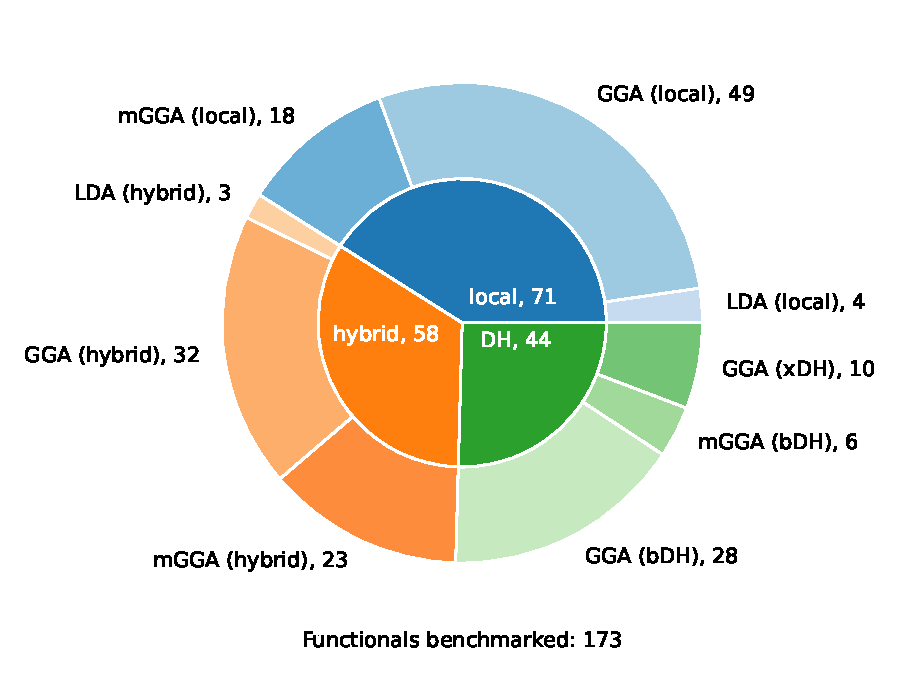
\includegraphics[width=0.6\textwidth]{assets/functionals-distribution.pdf}
\end{figure}

\subsection{径向函数与密度测评标准定义}

本工作所采用的测评标准与 Medvedev 等人的工作\cite{Medvedev-Lyssenko.S.2017}一致,通过分析密度格点的 RDF 以作评测。该 RDF 的坐标选取为以原子核为中心均匀分布的 0 -- 10 \AA 的 50000 个格点。

在特定密度矩阵 $D_{\mu \nu}$ 下,电子云密度 $\rho(\bm{r})$ 定义为
\begin{equation}
    \rho(\bm{r}) = \sum_{\mu \nu} D_{\mu \nu} \phi_{\mu} (\bm{r}) \phi_{\nu} (\bm{r})
\end{equation}
对于原子体系,上述函数仅与电子到原子核距离 $r$ 有关,因此上述密度也写为 $\rho(r)$。密度径向函数 RHO、梯度 GRD 与二阶梯度 LR 分别定义为
\begin{align}
    \text{RHO}(r) &= 4 \pi r^2 \rho(r) \\
    \text{GRD}(r) &= 4 \pi r^2 | \nabla \rho(r) | = 4 \pi r^2 \left| \frac{\partial \rho(r)}{\partial r} \right| \\
    \text{LR}(r) &= 4 \pi r^2 \nabla^2 \rho(r) = 4 \pi r^2 \frac{\partial^2 \rho(r)}{\partial r^2}
\end{align}
对于给定的性质 $P \in \{\text{RHO}, \text{GRD}, \text{LR}\}$、原子或离子 $a \in \{\ce{Be^0}, \ce{B^+}, \cdots, \ce{Ne^8+}\}$、以及泛函近似或 post-HF 方法 $f, g$,RMSD 误差定义为
\begin{equation}
    \text{RMSD}_{P, a, (f, g)} = \sqrt{\frac{1}{N} \sum_i^N \big(P_{a, f} (r_i) - P_{a, g} (r_i) \big)^2}
\end{equation}
其中 $N = 50000$ 为格点数。特别地,若 $g = \textsf{CCSD}$,则简记 $\text{RMSD}_{P, a, f} = \text{RMSD}_{P, a, (f, \textsf{CCSD})}$。为了合理地将不同性质的误差作公平的对比,上述的 RMSD 误差将除以性质均值数 median RMSD,得到均值数归一后的方均误差 MNAE:
\begin{equation}
    \text{MNAE}_{P, a, (f, g)} = \frac{\text{RMSD}_{P, a, (f, g)}}{\text{median}_{P} \text{RMSD}_{P, a, (f, g)}}
\end{equation}
最后,通过对原子指标 $a$ 求取极大值或平均值,可以得到泛函或方法 $f$ 在性质 $P$ 上的表现:
\begin{align}
    \text{maxMNAE}_{P, (f, g)} &= \max_a \text{MNAE}_{P, a, (f, g)} \\
    \text{meanMNAE}_{P, (f, g)} &= \underset{a}{\text{mean}} \, \text{MNAE}_{P, a, (f, g)}
\end{align}

本工作的 median RMSD,对于 RHO (单位 $\text{e} \, \text{\AA}^{-1}$) 为 0.009943368,对于 GRD (单位 $\text{e} \, \text{\AA}^{-1} \, \text{Bohr}^{-1}$) 为 0.092398036,对 LR (单位 $\text{e} \, \text{\AA}^{-1} \, \text{Bohr}^{-2}$) 为 1.445110833\footnote{在 Medvedev 等人的工作\cite{Medvedev-Lyssenko.S.2017} 中,用于图片展示的 GRD 的单位是 $\text{e} \, \text{\AA}^{-2}$、LR 的单位是 $\text{e} \, \text{\AA}^{-3}$;但我们的验证认为其单位换算可能存在问题。尽管如此,由于实际用于衡量泛函或方法间误差与优劣的标准是无量纲的 maxMNAE 或 meanMNAE,因此物理单位的问题不影响结论与讨论。}。

\section{测评结果}

完整的测评结果参考附录的表 \ref{tab.full-atom-benchmark}。由于数据较多,后文将对该表格的结果作分析与讨论。

\subsection{依年代发展的总体表现}

\begin{figure}[tp]
    \centering
    \caption{诸泛函密度径向函数最大均值数归一方均误差 (maxMNAE) 对其年代的散点图。实线表示的平均值曲线是通过对年代作 5 年为期的二次平均所得,因此反映的是前后 10 年左右的总体趋势变化。交换泛函中,局域部分所对应的泛函类型 (LDA、GGA、meta-GGA 或 mGGA) 以散点形状 (三角、叉号、加号) 区分;非局域部分 (无非局域、杂化、双杂化) 以颜色 (蓝色、橙色、绿色) 区分。由于部分数据点误差较大,在 GRD 图中 M11-L, N12, N12-SX, MN15, MN15-L 五个泛函、以及 LR 图中 M11-L, MN12-L, MN12-SX, MN15, MN15-L 五个泛函未展示在图中。}
    \label{fig.maxMNAE-against-year}
    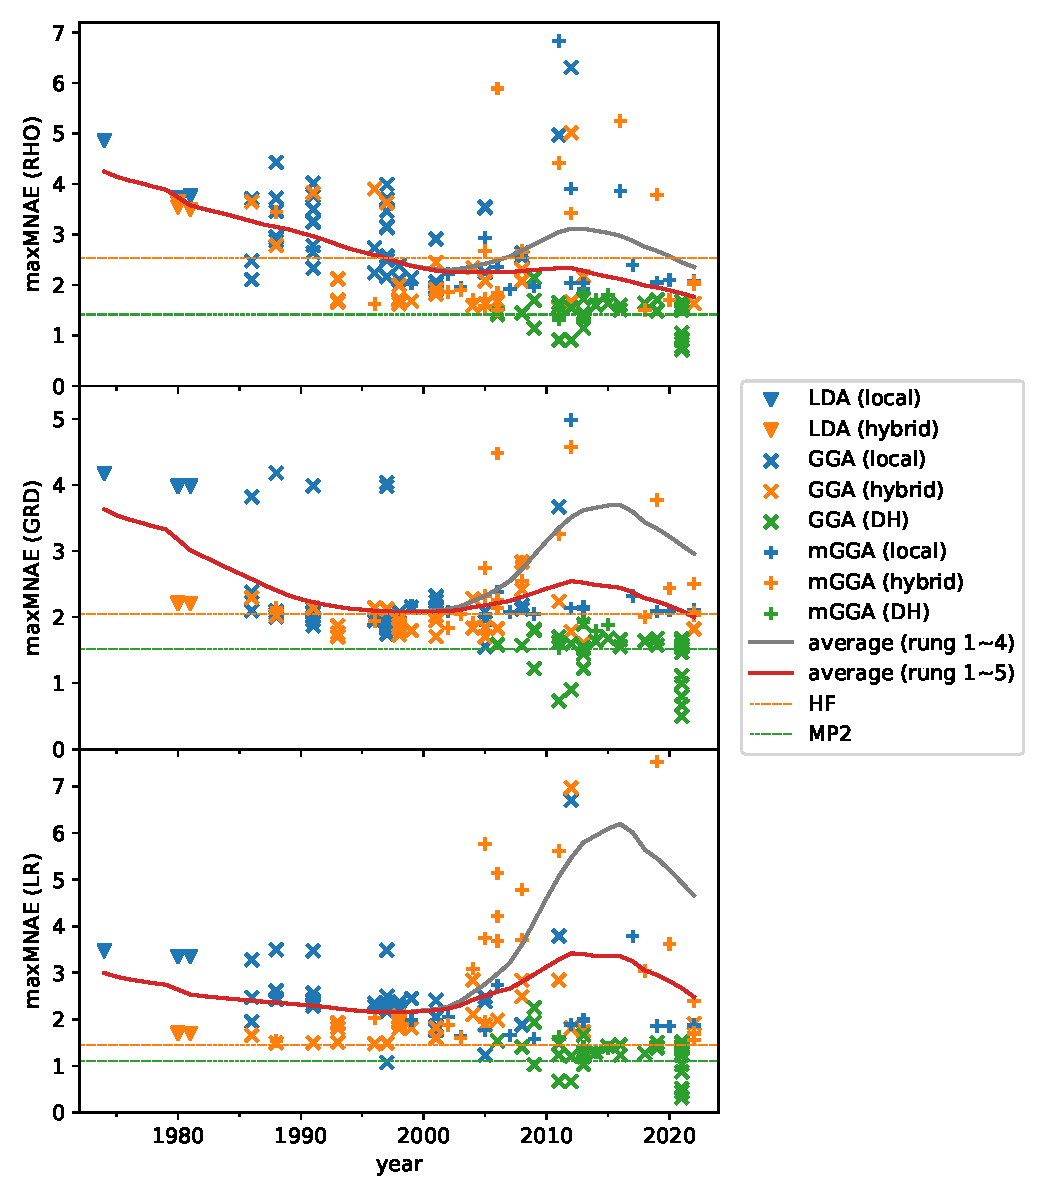
\includegraphics[width=0.8\textwidth]{assets/maxMNAE-against-year.pdf}
\end{figure}

Medvedev 等人工作的 Fig.\ 1 中,展现了随着年代的发展,泛函在密度径向函数 RHO 的测评上,平均误差在 2003 年左右先逐渐减小、尔后到 2015 年显著增大的情况。基于我们的测评,在图 \ref{fig.maxMNAE-against-year} 中,我们复现了这一趋势、并且对该图像作了拓展。图 \ref{fig.maxMNAE-against-year} 的灰色实线是“Jacob 阶梯”上低阶泛函依发展年代平均下密度径向函数的 maxMNAE 误差表现。相比于 Medvedev 等人的工作中,看到低阶密度泛函近似逐渐偏离正确结果的结论,我们看到误差在 2015 年达到高点以后逐渐下降的趋势。因此,从现在的眼光来看,低阶密度泛函近似确实回到了正确的道路上。

除此之外,我们补充了双杂化密度泛函近似的结果。图 \ref{fig.maxMNAE-against-year} 的红色实线体现了“Jacob 阶梯”上所有泛函近似依发展年代平均下密度径向函数的 maxMNAE 误差表现。Medvedev 等人的工作指出,在 2005 年以前,泛函近似大体上依“Jacob 阶梯”的爬升而在密度径向函数上的误差次第降低。而从图 \ref{fig.maxMNAE-against-year} 中,我们看到作为“Jacob 阶梯”上更高级别的方法啊,双杂化泛函相比于低阶泛函,其误差有显著的进一步降低。被测评的所有低阶泛函中,没有泛函在密度的表现上超越 MP2 方法;但不少双杂化泛函的表现相较于 MP2 更好。因此,尽管双杂化泛函付出了一定程度的计算代价,引入了对大体系而言计算量较大的 MP2 型相关能、以及对小体系而言计算量较大的密度泛函近似;但密度表现上有显著提升,同时好于低阶的泛函或 MP2 方法。

与此同时注意到,对于图 \ref{fig.maxMNAE-against-year},局域、杂化与双杂化泛函三个层级之间有较为明显的差别;但在每个层级内部,对于泛函是否掺杂 LDA、GGA 或 meta-GGA 形式的近似,影响不是非常显著。这表明,总体上来说,相比于引入局域信息仔细程度的多寡而言,泛函包含多少程度的非局域信息,将比较显著地影响泛函近似在密度上的测评结果。由于双杂化泛函同时包含了交换与相关两者的非局域效应,因此更有可能给出更好的密度表现。但同时需要指出,Medvedev 等人 Fig.\ 2 附近的讨论中,表明对于交换能,并非引入愈多的非局域杂化效应,密度上的表现愈好;引入适当的非局域效应才能正确描述密度性质。

除了密度性质外,在图 \ref{fig.MAE-etot-against-year} 中,我们也对诸泛函在离子体系的 $1s^2 2s^2 \rightarrow 1s^2$ 过程的电离能问题的表现作依年代发展的测评。从年代的发展趋势来看,泛函近似的误差走势在原子电离能测评上与密度测评近乎一致,但细节的结构上有比较明显的不同。相比于密度的测评表现,对于原子的电离能,尽管一般来说包含愈多的非局域信息 (即泛函从“Jacob 阶梯”的第 1--3 阶爬升到第 4 到第 5 阶) 通常有愈稳定且愈低的误差,但这种优势并非是绝对的。事实上,如果仅从表现最优异的泛函来看,甚至结论是相反的:不含任何杂化的 PBELYP (MAD 误差 0.12 eV) 比杂化泛函 M06-2X (MAD 误差 0.23 eV) 比双杂化泛函 revXYG3 (MAD 误差 0.31 eV) 要更为精确。但一方面,误差较大的泛函通常是低阶泛函、而高阶泛函在电离能上的表现可以保证稳定地好于 HF 方法。而另一方面,对于低阶泛函,不少情形下可以对能量或密度的其中一者有良好的描述,但往往难以同时对两者都有出色的表现。以上面列举的三个泛函为例,若以 RHO、GRD、LR 三者的 maxMNAE 取最大值作为密度径向函数的测评标准,则 revXYG3 (1.113) 比 PBELYP (3.710) 比 M06-2X (4.214) 要更为出色。双杂化泛函则确实可以在平衡能量和密度误差的同时,对两者同时有显著的提升。

\begin{figure}[t]
    \centering
    \caption{诸泛函密度电离能平均误差 MAE 对其年代的散点图。图例参考图 \ref{fig.maxMNAE-against-year}。}
    \label{fig.MAE-etot-against-year}
    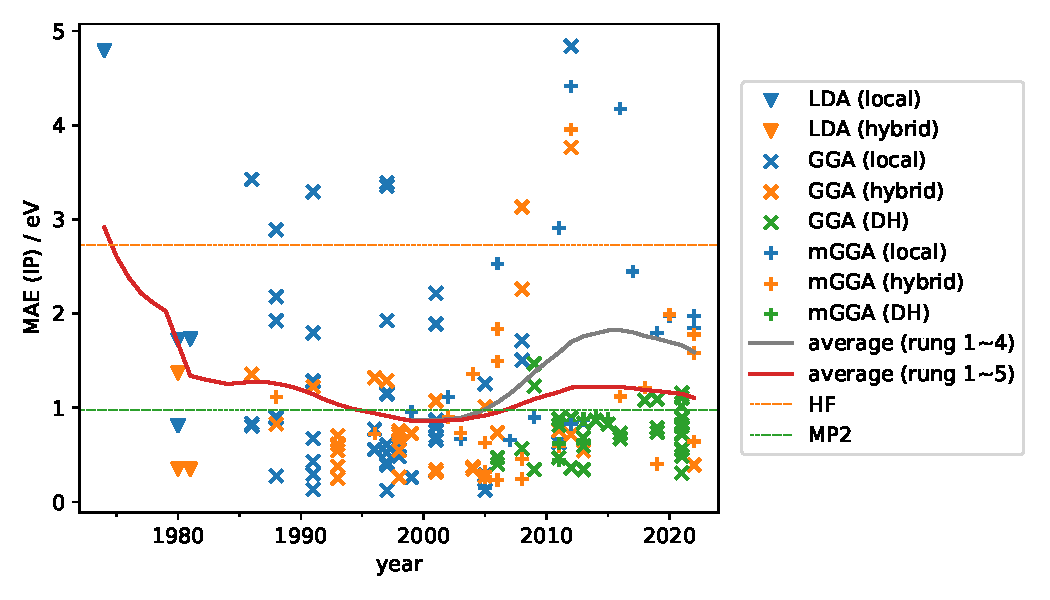
\includegraphics[width=0.7\textwidth]{assets/MAE-etot-against-year.pdf}
\end{figure}

\subsection{具体测评表现}

这里我们将更具体地讨论泛函的测评误差表现。

密度径向函数的测评包含三个指标,即 RHO ($\rho(\bm{r})$)、GRD ($|\nabla \rho(\bm{r})|$) 与 LR ($\nabla^2 \rho(\bm{r})$)。由于这些指标之间有比较强的相互关联,因此泛函在其中一个指标上的表现若更好,往往也在其他的指标上有不错的表现。图 \ref{fig.compare-err-RHO-GRD} 作为一个离子,对 RHO 与 GRD 的指标误差进行绘制,可以印证上述结论。同时注意到,相比于局域与杂化泛函而言,双杂化泛函在不同的密度径向函数误差指标上的一致性更强,即在图 \ref{fig.compare-err-RHO-GRD} 上代表双杂化泛函的散点更靠近黑色的实线。

\begin{figure}[t]
    \centering
    \caption{诸泛函密度径向函数测评的 $\text{maxMNAE}_\text{RHO}$ 与 $\text{maxMNAE}_\text{GRD}$ 对照图。}
    \label{fig.compare-err-RHO-GRD}
    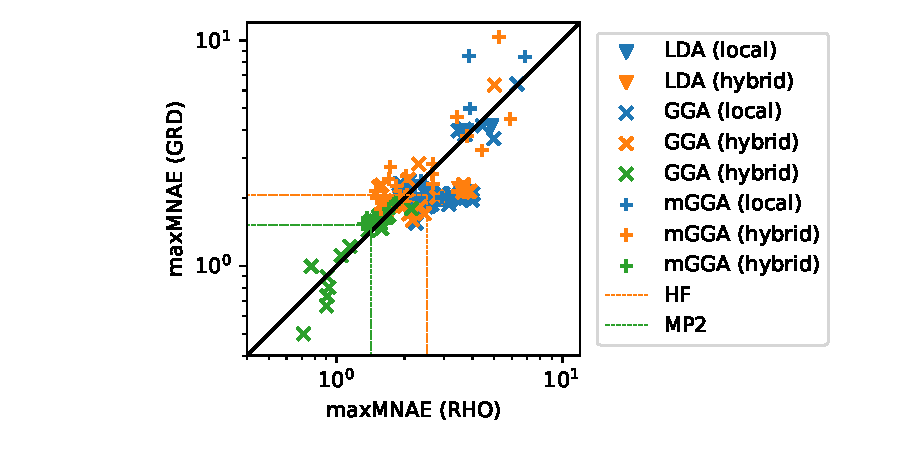
\includegraphics[width=0.6\textwidth]{assets/compare-err-RHO-GRD.pdf}
\end{figure}

但类似的情况,对于电离能和密度径向函数的比较上并不成立。以图 \ref{fig.compare-err-maxMNAE-MAEIP} 为例,尽管大多数泛函大体上在当密度表现较好时,电离能的表现也较好;但注意到低阶的局域与杂化泛函中,不少在能量表现上优异、但在密度表现则稍差。图 \ref{fig.compare-err-maxMNAE-MAEIP} 中橙色虚线表示 HF 方法的误差;我们发现绝大多数能量误差最低的泛函 (包括 PBELYP (0.12 eV), mPWLYP1w (0.12 eV), PW91LYP (0.13 eV), TPSSLYP1w (0.15 eV), M06-2X (0.23 eV), M08-SO (0.25 eV) 等) 的密度误差显著地大于 HF 方法。一般来说,以 maxMNAE 为考察标准,重参数拟合的泛函如 M08-SO (4.78), M06-2X (4.21) 的误差要大于少参数或无参数泛函如 PBELYP (3.71), mPWLYP1w (3.53);这在 M11-L (16.27) 与 MN12-SX (13.00) 等泛函体现地更为明显。对于能量表现良好、但密度表现较差的泛函,我们认为这是由于密度 $\rho$ 的误差与能量泛函的误差 $E[\rho]$ 相互抵消所致;正确的结果不能因为两次错误恰好相互抵消,而就这样认为能量结果导出的过程便是正确的\cite{Hammes-Schiffer-Hammes-Schiffer.S.2017, Korth-Korth.ACIE.2017, Graziano-Graziano.NRC.2017};一旦泛函的优化方式有所改变,原本有可能正确的能量,很可能会产生严重的错误 (以电离能的 MAE 作为测评标准,尽管 M06-2X 误差很小,但其衍生发展的泛函误差相当大,其中 M11-L 误差 2.91 eV、MN12-SX 误差 3.96 eV)。而 B3LYPV1R (Gaussian 与 LibXC 默认的 B3LYP 方法,0.25 eV) 与 mPW1LYP (0.26 eV) 等泛函近似的密度误差 (以 maxMNAE 评测) 也小于 HF 方法;这些泛函在与 HF 方法计算量相当的前提下,可以认为有效地同时处理好密度与能量的计算。

\begin{figure}[t]
    \centering
    \caption{诸泛函密度径向函数测评的 $\text{maxMNAE}$ 与电离能的平均绝对值误差 (MAE) 对照图。这里的 maxMNAE 是指三个密度测评指标 $\text{maxMNAE}_\text{RHO}$、$\text{maxMNAE}_\text{GRD}$、$\text{maxMNAE}_\text{LR}$ 的最大值。}
    \label{fig.compare-err-maxMNAE-MAEIP}
    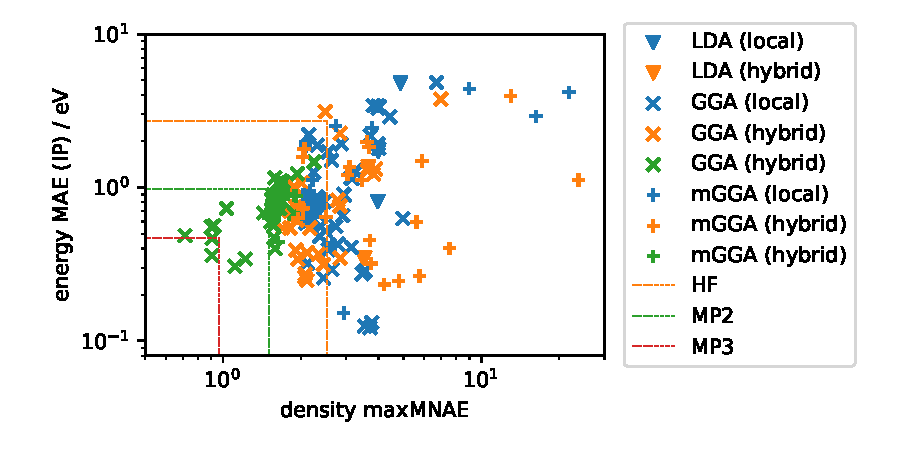
\includegraphics[width=0.6\textwidth]{assets/compare-err-maxMNAE-MAEIP.pdf}
\end{figure}

但我们同时注意到,目前没有任何低阶的局域与杂化泛函,在密度的表现上 (以 maxMNAE 评测) 可以优于 MP2 方法。这个情形不仅在 2015 年以前发展的低阶泛函成立,也在 2015 年以后发展的低阶泛函成立。但对于双杂化泛函而言,一方面不少泛函的密度与能量误差同时小于或接近 MP2 方法的级别;即使超出了 MP2 的误差,也通常不会大于 HF 方法的误差。因此,目前所有双杂化泛函的密度与能量都可以认为比较可靠。另一方面,revXYGJ-OS, XYG6, xDH-PBE0, XYGJ-OS, XYG5 等五个泛函的能量与密度的表现甚至超越了 MP3 方法;因此,双杂化泛函有希望以较低的代价,同时在密度与能量的表现上逼近计算量更为庞大的波函数方法。

\begin{figure}[t]
    \centering
    \caption{双杂化泛函密度径向函数测评的 $\text{maxMNAE}$ 与电离能的平均绝对值误差 (MAE) 对照图。这里的 maxMNAE 是指三个密度测评指标 $\text{maxMNAE}_\text{RHO}$、$\text{maxMNAE}_\text{GRD}$、$\text{maxMNAE}_\text{LR}$ 的最大值。}
    \label{fig.compare-err-maxMNAE-MAEIP-dh}
    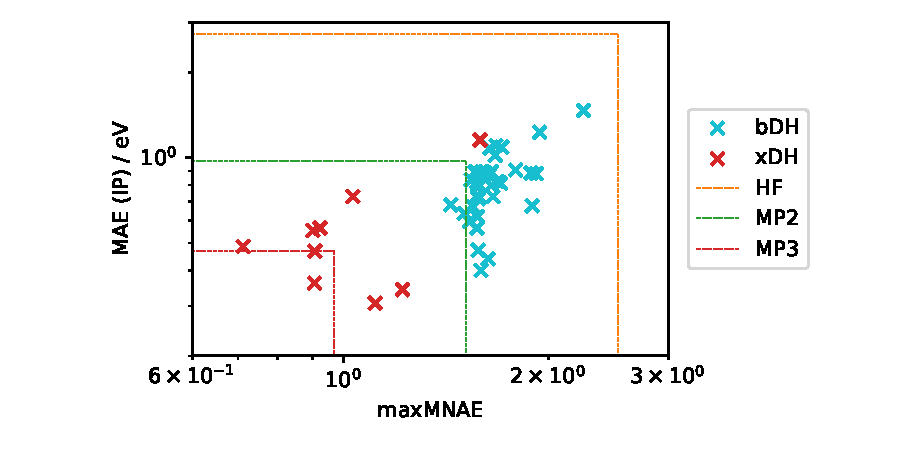
\includegraphics[width=0.6\textwidth]{assets/compare-err-maxMNAE-MAEIP-dh.pdf}
\end{figure}

在双杂化泛函中,XYG3 型 (xDH) 泛函的表现与 B2PLYP 型 (bDH) 泛函的表现也有所差异。图 \ref{fig.compare-err-maxMNAE-MAEIP-dh} 与图 \ref{fig.compare-err-maxMNAE-MAEIP} 相同,但仅绘制双杂化泛函的数据,并区分 xDH 型与 bDH 型泛函。可以看到,xDH 型泛函不仅在能量、也同时在密度上,有着比 bDH 型泛函更优异的表现。在 bDH 型泛函中,仅有 DSD-PBEPBE-D3BJ 与 DSD-PBEB95-D3BJ 相较于 MP2 而言有更优异的密度与能量表现;但除 XYG7 外的所有测评的 xDH 型泛函,其表现都优于 MP2 方法,且也与 DSD 系列泛函拉开了一定的差距。

\section{讨论与本章小结}

\begin{figure}[t]
    \centering
    \caption{部分泛函的密度径向函数最大误差 maxMNAE 与电离能平均绝对误差 MAD 测评表现示意图。线图 (maxMNAE) 的误差是指三个密度测评指标 $\text{maxMNAE}_\text{RHO}$、$\text{maxMNAE}_\text{GRD}$、$\text{maxMNAE}_\text{LR}$ 的最大值。柱状图 (电离能误差) 的零点选取为 MP2 的误差 (0.973 eV)。对于特定泛函近似,只有其在图上对应的条形柱与散点都在红色五角星标识的 MP2 误差的情形下,该方法才能被认为同时在电离能与密度径向函数的表现上都优于 MP2 方法。}
    \label{fig.compare-err-relative}
    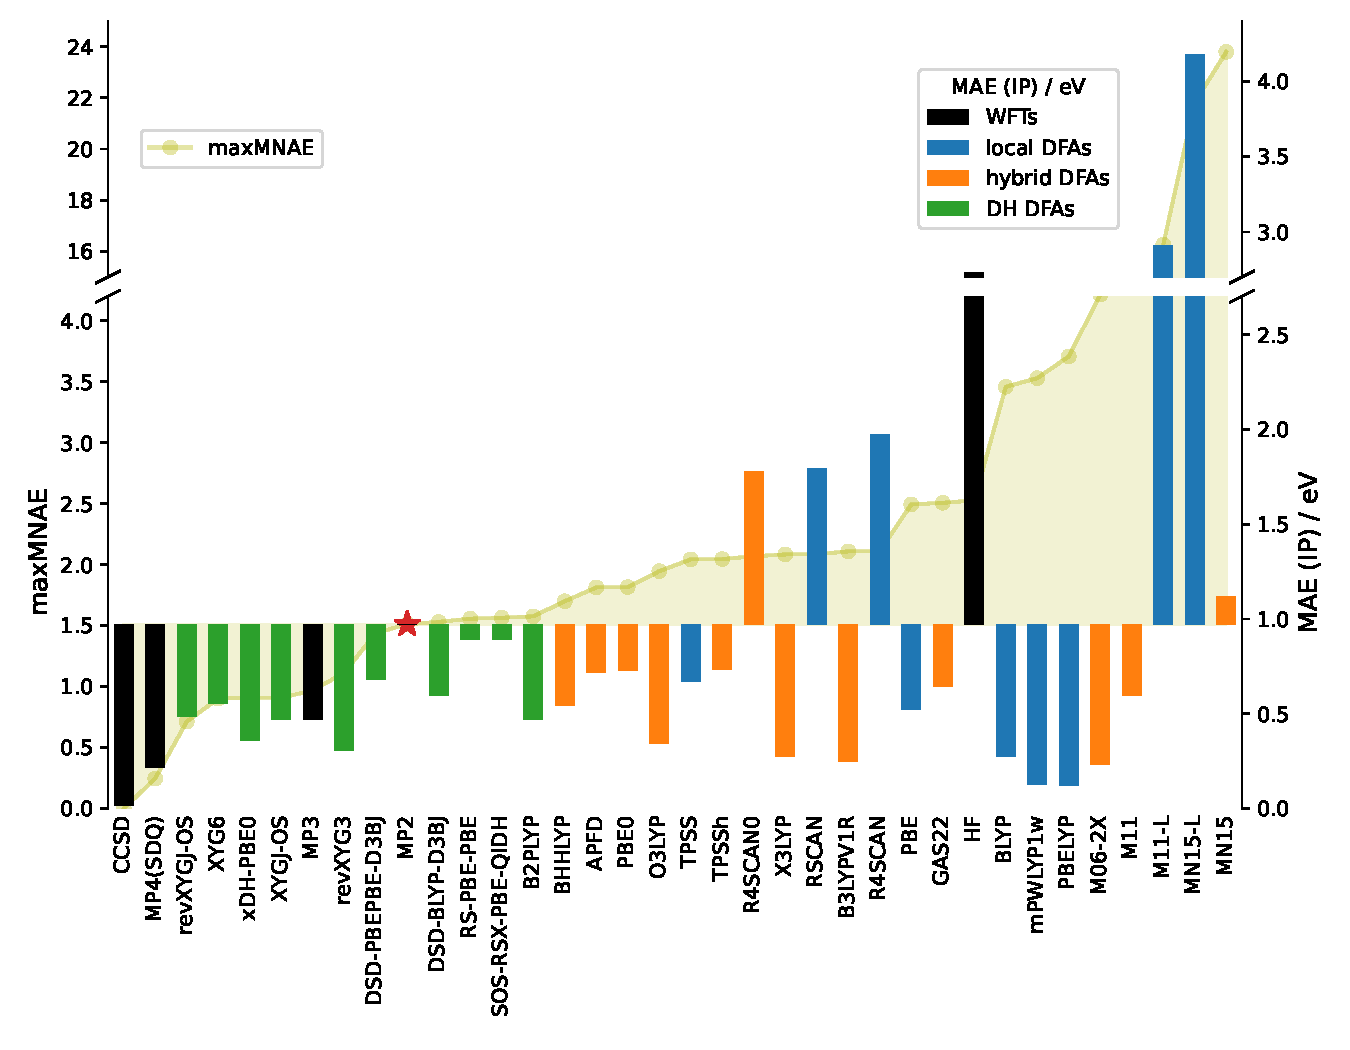
\includegraphics[width=0.9\textwidth]{assets/compare-err-relative.pdf}
\end{figure}

上面的结果分析,确实地验证了当前双杂化泛函、特别是 xDH 型双杂化泛函,在原子体系的电离能与电子云密度上有良好的表现。作为具体的例子,部分泛函的测评结果用更加直观的方式,呈现在图 \ref{fig.compare-err-relative} 中。需要注意到,所有本章涉及到的密度泛函,都并未专门针对这些测评标准所优化;因此几乎不存在因为经验参数拟合而有更好表现的可能——良好的测评表现更适合归因于泛函本身的优势。

Medvedev 等人的工作也已经表明,除了少数特定的泛函,泛函的“Jacob 阶梯”越高、电子云密度表现越好。我们注意到特别在电子云密度的表现上,作为“Jacob 阶梯”上最高的类别,双杂化泛函相比于其他泛函都有明显的优势;从而我们的工作印证并延伸了 Medvedev 等人的结论。因此,对于 xDH 型泛函,其优势之一在于它是“Jacob 阶梯”最高阶的双杂化泛函。

而其优势之二在于,它提供了一种切实可行、易于实现的同时矫正能量与密度误差的方案。现在一种普遍接受与流行的观点是,密度泛函近似存在两个误差来源:一是能量驱动误差、二是密度驱动误差。一般来说,能量驱动误差更为关键\cite{Cohen-Yang.CR.2012};但在一些的情况下,密度驱动的误差也会产生重要的影响\cite{Kim-Burke.JCP.2014}。事实上,这两种误差在标准的 Kohn-Sham 框架下是相互耦合的:欠佳的交换相关泛函将会给出欠佳的能量;而对这个欠佳的能量作变分,将会给出偏离真实的 Kohn-Sham 势函数,进而无法给出真实精确地密度。因此,能量与密度通过 Kohn-Sham 势函数得以联系起来\alert{第二章公式 eq.v-x, eq.v-c-lambda}:
\begin{equation}
    v_\mathrm{xc} (\bm{r}) = v_\mathrm{x} (\bm{r}) + v_{\mathrm{c}, \lambda=1} (\bm{r}) = \frac{\delta E_\mathrm{xc} [\rho]}{\delta \rho(\bm{r})}
\end{equation}
或者在 Generalized Kohn-Sham 理论下,将 $E_\mathrm{xc}$ 看作双粒子密度的泛函 (而并非是局域的关于 $\bm{r}$ 函数的泛函) 时,能量与密度通过下述势函数得以联系:
\begin{equation}
    v_\mathrm{xc}^\mathrm{GKS} (\bm{r}, \bm{r}') = \frac{\delta E_\mathrm{xc}}{\delta \rho(\bm{r}, \bm{r}')}
\end{equation}
后者实际上已经突破了 Kohn-Sham 理论框架本身了\cite{Su-Xu.WCMS.2016, Su-Xu.IJQC.2015, Su-Xu.MP.2016}。对于“Jacob 阶梯”上第五阶泛函,它并非表示为密度 $\rho(\bm{r})$ 或密度矩阵 $D_{\mu \nu}$ 的显式泛函;而这应当是真实泛函的特征\cite{Kohn-Kohn.PRB.1986, Yang-Mori-Sanchez.JCP.2012}。对于 xDH 型泛函,其使用较低阶的泛函近似,大体上可信与精确、但同时又以良好效率性价比地给出密度与轨道信息;而同时,在最终能量计算时,则引入更高阶的双杂化泛函近似形式,以通过引入非局域相关能效应 (也是 GKS 框架下泛函应当具有的特性) 的方式,进一步提升能量计算的精度。低阶泛函自洽场的电子云密度,则可以通过高阶能量泛函相对于自洽场泛函之差所给出的微扰,以 Z-Vector 方法矫正\cite{Handy-Schaefer.JCP.1984, Su-Xu.JCC.2013}。相比之下,低阶泛函所包含的非局域信息不足;而 bDH 型泛函则在自洽场泛函中没有引入完整的相关效应,因此自洽场所给出的密度也缺失一些相关效应。正因为 xDH 型泛函近似在框架设计上克服了上述两类泛函的困难,可以对能量与密度两者分别作精度的调整与提升;从而,xDH 型泛函近似相比于其他低阶泛函近似、以及 bDH 型双杂化泛函近似,更有可能同时在能量与密度上有良好的表现。

对于低阶泛函普遍逊色于高阶泛函、特别是 xDH 型泛函;我们作如下理解。从分数电荷的表现上,xDH 型泛函表现显著地好于传统泛函\cite{Su-Xu.IJQC.2015, Su-Xu.WCMS.2016, Su-Xu.MP.2016, Su-Xu.ARPC.2017},即更接近 PPLB 定理所要求的直线型分数电离趋势\cite{Perdew-Balduz.PRL.1982}。作为第四阶的杂化泛函,分数电荷表现欠佳;这可以归因于非局域的严格交换效应没有很好地被非局域的相关效应所平衡;而 MP2 型相关效应,作为一种非局域相关效应,其引入可以很大程度上缓解分数电荷的计算误差。分数电荷在概念上与电子云有密切的联系,因此上述讨论,很可能适用于对以 xDH 型泛函为代表的双杂化泛函,在密度表现上断档式地好于低阶泛函,这种现象的一种解释。

作为展望,“Jacob 阶梯”不仅是对现有的泛函近似的一种归类方式,同样也是对未来泛函发展思路的一种指导。一方面,对于分子体系计算,从泛函近似的发展上、或从计算可行性上,引入严格交换能已经成为比较普遍的共识;因此,如果泛函近似还有哪些不足,则应该认为在相关贡献上有更多文章可作。为拓展泛函近似的可能性,作为一条前进的道路,在本论文的第二章中,我们尝试了 IEPA 型,以避免 MP2 型相关能在 HOMO/LUMO gap 过小的体系的误差。我们也期待在“Jacob 阶梯”的最高阶上有更多的工作,以拓展双杂化泛函的应用范围,在计算量可接受的方法与算法下,其能量与性质越来越接近普适泛函、达到梦想的化学精度。

\section{附录}

\subsection{密度径向函数的 RI 近似误差}

我们对 HF 与 MP2 方法的 RI 近似在密度径向函数上的误差作简要的评测与分析。在本评测中,参考值取为非 RI 近似 (传统 ERI 积分) 的情形,而非以 CCSD 精确地密度作为参考。我们仅针对 aug-cc-pV$X$Z 与 aug-cc-p$\omega$CV$X$Z ($X=\mathrm{D,T,Q,5}$) 作测评。该小节不考察 Be 原子,即总共考察 13 个原子或离子体系。

HF 方法的 RI 近似也即 RI-JK 方法。我们分别考察了 aug-cc-pV$X$Z-jkfit 辅助基\cite{Weigend-Weigend.PCCP.2002}与自动生成辅助基 ETB\cite{Stoychev-Neese.JCTC.2017}的表现。在图 \ref{fig.HF-RI-err} 与 \ref{fig.HF-RI-mean} 中,可以看出,RI 近似对于 HF 方法的密度径向函数所引入的误差,在所有体系下 MNAE 最大不超过 $2 \times 10^{-3}$。由于泛函近似或 post-HF 方法与与 CCSD 之间的密度径向函数误差通常大于 0.1,因此 RI 所引入的误差完全可以忽略。同时,我们注意到普遍来说,通过对库伦与交换能作数值优化的 aug-cc-pV$X$Z-jkfit 基组尽管大小较小,但误差相比于自动生成的 ETB 基组要更大一些。ETB 基组的误差通常随着基组的增大 (基数 $X$ 的增大) 而减小。

\begin{figure}[t]
  \centering
  \caption{HF 方法 RI 近似下的 maxMNAE 误差。}
  \label{fig.HF-RI-err}
  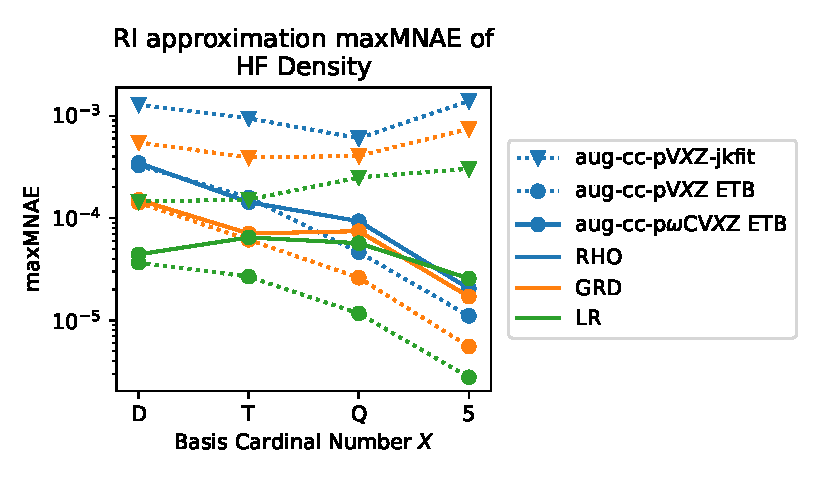
\includegraphics[width=0.7\textwidth]{assets/HF-RI-err.pdf}
\end{figure}

\begin{figure}[t]
  \centering
  \caption{HF 方法 RI 近似下的 meanMNAE 误差。}
  \label{fig.HF-RI-mean}
  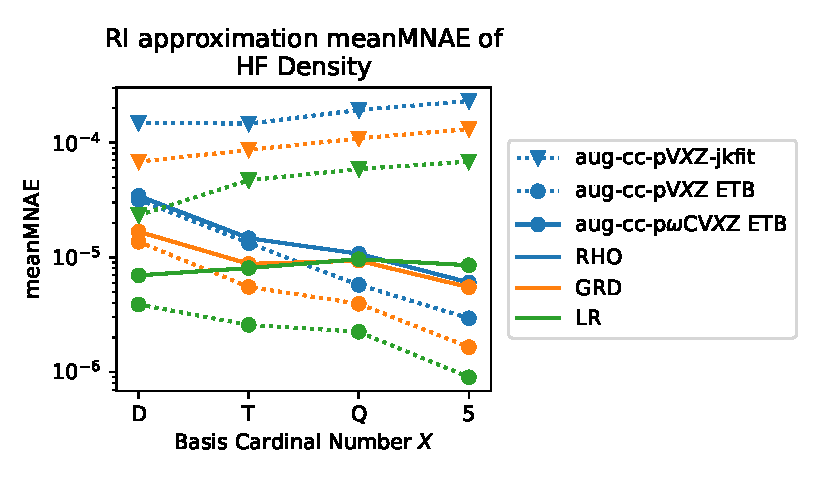
\includegraphics[width=0.7\textwidth]{assets/HF-RI-mean.pdf}
\end{figure}

对于 MP2 方法而言,我们也分别考察了 aug-cc-pV$X$Z-rifit 辅助基\cite{Weigend-Haettig.JCP.2002}、aug-cc-p$\omega$CV$X$Z 辅助基\cite{10.1039/b415208e}与自动辅助基 ETB\cite{Stoychev-Neese.JCTC.2017}的表现。这里自洽场部分使用传统 ERI 积分实现,以保证 RI 近似误差仅出现在 MP2 的相关贡献部分。在图 \ref{fig.MP2-RI-err} 与 \ref{fig.MP2-RI-mean} 中,可以看出,采用对 MP2 相关能作优化的 aug-cc-pV$X$Z-rifit 辅助基或 aug-cc-p$\omega$CV$X$Z 辅助基时,密度梯度径向函数 GRD 与二阶梯度径向函数 LR 的误差会较大;对于 GRD,其最大的 MNAE 误差可以达到 0.9;这将会影响泛函或方法在密度径向函数上的评测准确性。相较而言,自动生成辅助基 ETB 方案将给出小于 $10^{-3}$ 的密度径向函数误差;这个误差不会影响测评表现。

\begin{figure}[t]
  \centering
  \caption{MP2 方法相关贡献 RI 近似下的 maxMNAE 误差。}
  \label{fig.MP2-RI-err}
  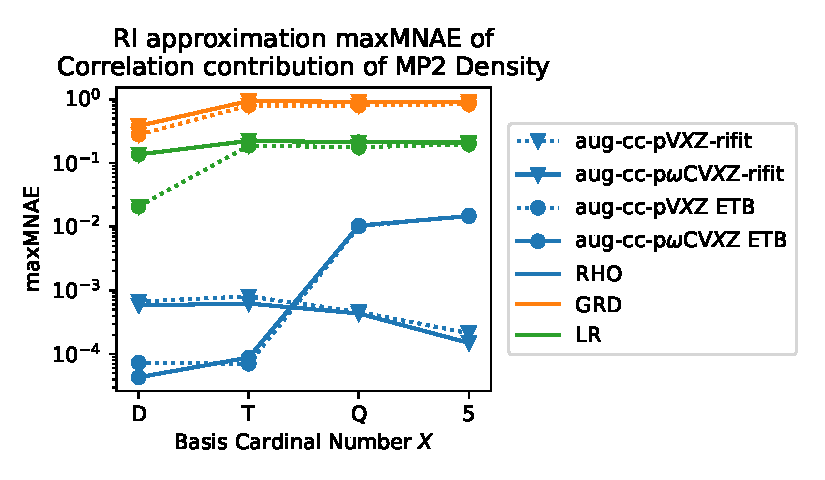
\includegraphics[width=0.7\textwidth]{assets/MP2-RI-err.pdf}
\end{figure}

\begin{figure}[t]
  \centering
  \caption{MP2 方法相关贡献 RI 近似下的 meanMNAE 误差。}
  \label{fig.MP2-RI-mean}
  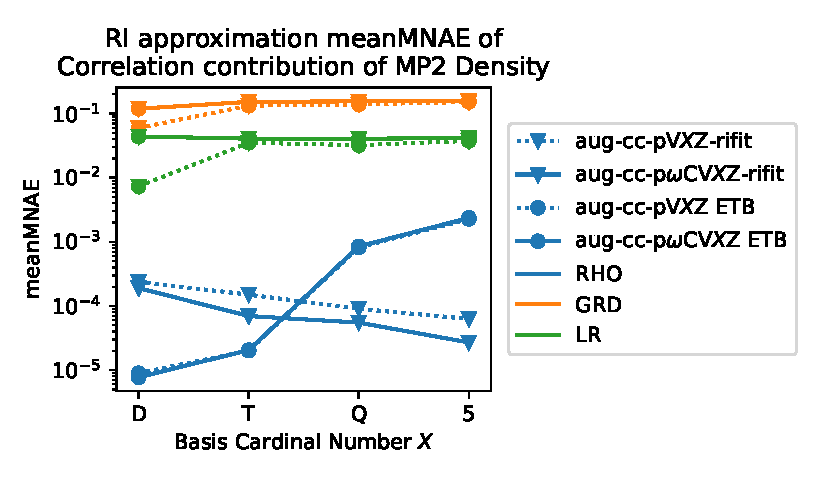
\includegraphics[width=0.7\textwidth]{assets/MP2-RI-mean.pdf}
\end{figure}

从上述简要的分析,我们认为,对自洽场与微扰部分使用自动生成辅助基的 ETB 方案、作 RI 近似,对密度径向函数的影响非常小以至于可以忽略;而采用预制的针对能量计算作优化的辅助基,对于自洽场部分的影响较小、但对微扰部分的影响较大以至于不能忽略。因此,在本工作中,我们统一使用 ETB 方案的辅助基。

\subsection{电离能的 RI 近似误差}

我们对 HF 与 MP2 方法的 RI 近似在离子电离能上的误差作简要的评测与分析。评测的方式与上一小节相似。该小节考察的体系是 \ce{Be^+}, \ce{C^2+}, \ce{N^3+}, \ce{O^4+}, \ce{F^5+}, \ce{Ne^6+} 六个离子体系电离两个电子,即 $1s^2 2s^2 \rightarrow 1s^2$ 的电离能。

从图 \ref{fig.HF-RI-eng} 与 \ref{fig.MP2-RI-eng} 可以看出,RI 近似对第二周期元素 $1s^2 2s^2 \rightarrow 1s^2$ 电离能所产生的误差总是小于 $5 \times 10^{-3} \, \text{eV}$;该程度的不影响测评结果。同时,我们注意到,与密度径向函数的情形不同,自动生成辅助基的 ETB 方案在 MP2 相关能计算上的误差,在 $X=\mathrm{T}$ 或更大的基组下,相比于预制辅助基而言要大。

\begin{figure}[t]
    \centering
    \caption{HF 方法 RI 近似下电离能最大误差。}
    \label{fig.HF-RI-eng}
    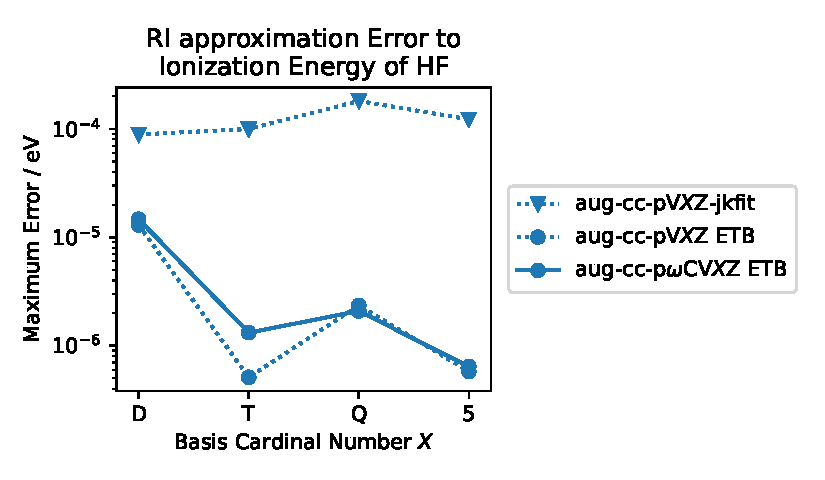
\includegraphics[width=0.7\textwidth]{assets/HF-RI-eng.pdf}
\end{figure}

\begin{figure}[t]
    \centering
    \caption{MP2 方法相关贡献 RI 近似下电离能最大误差。}
    \label{fig.MP2-RI-eng}
    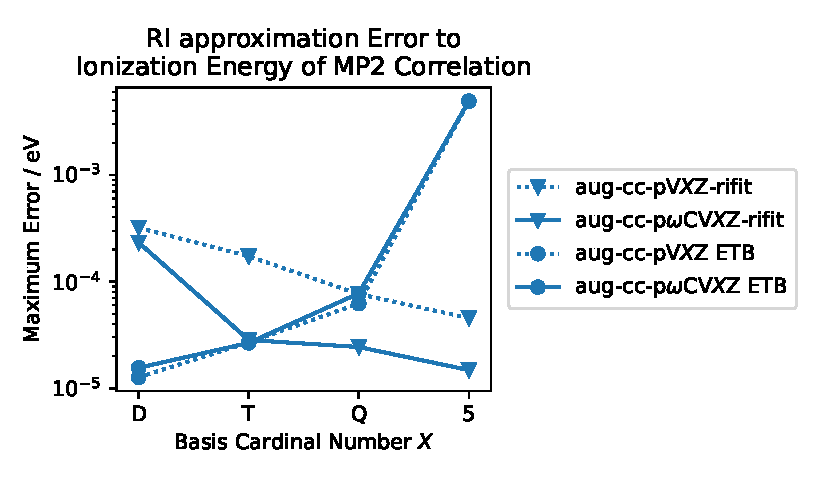
\includegraphics[width=0.7\textwidth]{assets/MP2-RI-eng.pdf}
\end{figure}

我们认为,对于杂化泛函或双杂化泛函,由于其严格交换能和微扰相关能贡献占比小于 100\%,从而 RI 近似对这部分能量或密度所产生的误差,预期不会比完整的 HF 和 MP2 方法更大。因此,我们认为可以在本工作的泛函测评过程中使用 RI 近似。

\subsection{密度径向函数测评的基组依赖性}

\begin{figure}[t]
    \centering
    \caption{诸泛函的密度径向函数在 aug-cc-p$\omega$CV5Z 与 aug-cc-pV5Z 基组下 maxMNAE 误差的比较。该图对横纵坐标使用对数坐标。}
    \label{fig.basisdep-RDF}
    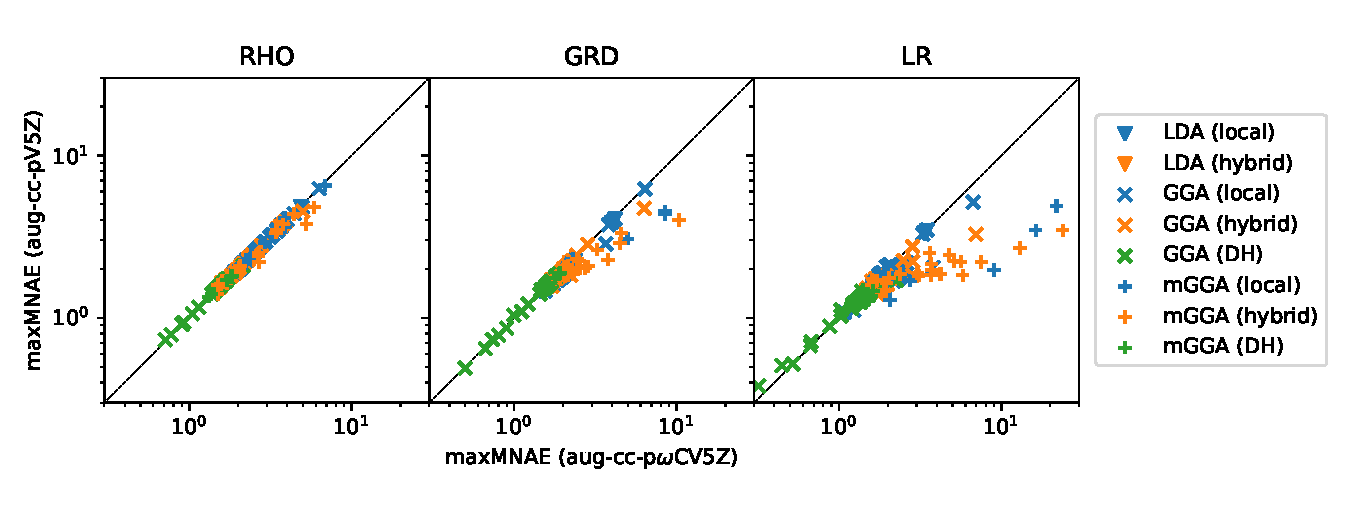
\includegraphics[width=0.95\textwidth]{assets/basisdep-RDF.pdf}
\end{figure}

王颖等人\cite{Wang-He.JCTC.2017}的工作指出,Medvedev 等人\cite{Medvedev-Lyssenko.S.2017}测评所使用的标准,在部分泛函上对基组的过于敏感。若测评所选用的基组从 aug-cc-p$\omega$CV5Z 降级为 aug-cc-pV5Z,尽管对大多数泛函不产生显著影响,但对部分泛函、特别是 Minnesota 系列泛函,其误差将显著降低。在图 \ref{fig.basisdep-RDF} 中\footnote{该图中的数据较多,但不适合放在论文的正文中。\alert{我们将会在 github 的仓库中展示绘制该图的具体数据。}},我们对所有泛函在这两个基组下的表现作测评。在该图中,若散点接近黑色虚线,则意味着泛函的密度径向函数误差不随基组的降级而产生明显变化。从该图中,我们可以看到的信息有
\begin{itemize}[nosep]
    \item 对于 $\text{maxMNAE}_\text{RHO}$ 与 $\text{maxMNAE}_\text{GRD}$ 的测评,绝大多数泛函在 aug-cc-p$\omega$CV5Z 与 aug-cc-pV5Z 基组的误差表现较为接近。
    \item 对于 $\text{maxMNAE}_\text{LR}$ 的测评,许多泛函,特别是 Minnesota 系列泛函的 aug-cc-pV5Z 误差显著地小于 aug-cc-p$\omega$CV5Z。从实用的角度上来说,Minnesota 系列泛函的适用情形是中等到大型分子体系的反应,主要关注电子的价层效应、而通常不必要使用专注于内核电子效应的 aug-cc-p$\omega$CV$X$Z 基组。因此,对于这类泛函,包括 Minnesota 系列泛函,使用 aug-cc-pV5Z 基组确实有其合理性。
    \item 从误差分析的角度上,aug-cc-p$\omega$CV5Z 基组所张成的空间比 aug-cc-pV5Z 要更大;而作测评时,若参考值足够准确,那么不论波函数或密度泛函近似方法,其误差总是包含方法误差、基组误差、与数值误差三者;当方法误差是着重关心的问题时,基组误差与数值误差应当越小越好。在假定数值误差足够小的前提下,基组误差是通过增大基组而减小的。使用基组 aug-cc-p$\omega$CV5Z 测评的结果应当更接近方法误差本身。由于我们工作的结果可以与其他工作合理地比对\cite{Medvedev-Lyssenko.S.2017, Kepp-Kepp.S.2017, Wang-He.JCTC.2017},因此预期数值误差较小。从而从误差分析的角度上,部分在 $\text{maxMNAE}_\text{LR}$ 指标上较差的泛函近似,确实应当归因于方法误差本身;这类泛函近似在更小的基组上有更好表现的现象,应当归结为方法误差与基组误差相抵消。
    \item 以绿色散点表示的双杂化泛函,在包括 $\text{maxMNAE}_\text{LR}$ 在内的所有密度径向误差指标上,aug-cc-p$\omega$CV5Z 与 aug-cc-pV5Z 基组的误差都较为接近。本工作着重关注双杂化泛函的测评表现;从图 \ref{fig.basisdep-RDF} 的表现上,我们认为使用不同 5-$\zeta$ 基组,不会影响先前文段的结论,即基组依赖性并不非常显著。
\end{itemize}

\subsection{其他补充数据}

\begin{itemize}[nosep]
    \item 所有经测评密度泛函近似的密度径向函数与电离能误差展示于表 \ref{tab.full-atom-benchmark};
    \item 部分低阶与双杂化泛函在 Be、Ne 原子上相对于 CCSD 方法的密度径向函数误差图展示于图 \ref{fig.supp-fig-s1} 与图 \ref{fig.supp-fig-s2}。其中,图 \ref{fig.supp-fig-s2} 应可与 Medvedev 等人\cite{Medvedev-Lyssenko.S.2017}工作的 Figs.\ S1--S3 作参考比较;
    \item 图 \ref{fig.supp-fig-s3} 与图 \ref{fig.supp-fig-s4} 展示了部分 xDH 型泛函相比于自洽场泛函,在密度径向函数上的提升情况。
\end{itemize}

\newpage

\begin{landscape}
\begin{longtable}{lc:cccc:rrr:rrr:rrr}
    \caption{诸泛函近似与波函数方法的原子密度径向函数与 $1s^2 2s^2 \rightarrow 1s^2$ 电离能测评详细数据。}
    \label{tab.full-atom-benchmark}
    \\ \hline
    &      &      & \multicolumn{3}{c}{hybrid}   & \multicolumn{3}{:c}{density   maxMNAE}  & \multicolumn{3}{:c}{density   meanMNAE}  & \multicolumn{3}{:c}{IP / eV}  \\
    functional & year & type\tabnote{a} & ex\tabnote{b} & corr\tabnote{c} & xDH & RHO               & GRD               & LR     & RHO                & GRD               & LR     & RMSE    & MAE   & MaxE  \\ \hline
    \endfirsthead
    \caption{(续表)}
    \\ \hline
    &      &      & \multicolumn{3}{c}{hybrid}   & \multicolumn{3}{:c}{density   maxMNAE}  & \multicolumn{3}{:c}{density   meanMNAE}  & \multicolumn{3}{:c}{IP / eV}  \\
    functional & year & type & ex & corr & xDH & RHO               & GRD               & LR     & RHO                & GRD               & LR     & RMSE    & MAE   & MaxE  \\ \hline
    \endhead
    \hline
    \endfoot
    \hline
    \endlastfoot
    %
    CCSD\tabnote{d} &      & WFT  &          &             &           & 0                 & 0                 & 0      & 0                  & 0                 & 0      & 0.017   & 0.016 & 0.023 \\
    MP4(SDQ)         &      & WFT  &          &             &           & 0.246             & 0.233             & 0.162  & 0.077              & 0.067             & 0.061  & 0.222   & 0.219 & 0.270 \\
    MP3              &      & WFT  &          &             &           & 0.881             & 0.967             & 0.718  & 0.339              & 0.254             & 0.149  & 0.481   & 0.469 & 0.621 \\
    MP2              &      & WFT  &          &             &           & 1.414             & 1.512             & 1.114  & 0.590              & 0.406             & 0.232  & 1.005   & 0.973 & 1.335 \\
    HF               &      & WFT  &          &             &           & 2.526             & 2.052             & 1.461  & 1.100              & 0.643             & 0.344  & 2.797   & 2.729 & 3.595 \\
    Slater           & 1974 & LDA  &          &             &           & 4.864             & 4.173             & 3.473  & 1.971              & 2.353             & 1.562  & 4.934   & 4.793 & 6.479 \\
    SVWN             & 1980 & LDA  &          &             &           & 3.725             & 3.983             & 3.349  & 1.591              & 2.100             & 1.402  & 1.885   & 1.718 & 2.882 \\
    SVWN1RPA         & 1980 & LDA  &          &             &           & 3.631             & 3.976             & 3.346  & 1.557              & 2.085             & 1.394  & 1.016   & 0.810 & 1.814 \\
    VWN1RPA          & 1980 & LDA  & exact    &             &           & 3.650             & 2.211             & 1.707  & 1.014              & 0.821             & 0.478  & 1.379   & 1.368 & 1.578 \\
    VWN5             & 1980 & LDA  & exact    &             &           & 3.540             & 2.203             & 1.694  & 1.020              & 0.808             & 0.469  & 0.410   & 0.348 & 0.627 \\
    PZ81             & 1981 & LDA  & exact    &             &           & 3.495             & 2.204             & 1.696  & 1.021              & 0.809             & 0.470  & 0.409   & 0.346 & 0.638 \\
    SPZ81            & 1981 & LDA  &          &             &           & 3.764             & 3.984             & 3.346  & 1.597              & 2.100             & 1.401  & 1.902   & 1.729 & 2.914 \\
    BP86             & 1986 & GGA  &          &             &           & 2.474             & 2.096             & 2.470  & 0.981              & 1.115             & 1.257  & 0.879   & 0.806 & 1.291 \\
    OP86             & 1986 & GGA  &          &             &           & 2.107             & 2.379             & 1.953  & 1.079              & 0.934             & 0.755  & 0.925   & 0.832 & 1.397 \\
    P86              & 1986 & GGA  & exact    &             &           & 3.650             & 2.294             & 1.659  & 1.220              & 0.830             & 0.467  & 1.471   & 1.355 & 2.169 \\
    SP86             & 1986 & GGA  &          &             &           & 3.709             & 3.820             & 3.277  & 1.753              & 2.193             & 1.468  & 3.608   & 3.425 & 5.061 \\
    BC               & 1988 & mGGA & exact    &             &           & 3.441             & 2.138             & 1.541  & 1.019              & 0.718             & 0.389  & 1.182   & 1.115 & 1.694 \\
    Becke            & 1988 & GGA  &          &             &           & 3.716             & 2.001             & 2.426  & 1.163              & 1.186             & 1.319  & 2.212   & 2.179 & 2.713 \\
    BLYP             & 1988 & GGA  &          &             &           & 3.458             & 2.050             & 2.455  & 1.055              & 1.196             & 1.330  & 0.332   & 0.274 & 0.569 \\
    BPZ81            & 1988 & GGA  &          &             &           & 2.956             & 2.087             & 2.608  & 0.927              & 1.242             & 1.399  & 0.893   & 0.892 & 0.921 \\
    BVWN             & 1988 & GGA  &          &             &           & 2.929             & 2.086             & 2.607  & 0.923              & 1.241             & 1.398  & 0.904   & 0.904 & 0.929 \\
    BVWN1RPA         & 1988 & GGA  &          &             &           & 2.870             & 2.094             & 2.616  & 0.915              & 1.246             & 1.403  & 1.925   & 1.924 & 1.968 \\
    LYP              & 1988 & GGA  & exact    &             &           & 2.786             & 2.021             & 1.496  & 0.984              & 0.633             & 0.367  & 0.922   & 0.826 & 1.450 \\
    SLYP             & 1988 & GGA  &          &             &           & 4.428             & 4.180             & 3.497  & 1.824              & 2.301             & 1.526  & 3.048   & 2.889 & 4.334 \\
    BPW91            & 1991 & GGA  &          &             &           & 2.330             & 1.956             & 2.329  & 0.956              & 1.092             & 1.220  & 0.720   & 0.672 & 1.049 \\
    PW91             & 1991 & GGA  &          &             &           & 2.642             & 1.870             & 2.285  & 0.994              & 1.107             & 1.214  & 0.342   & 0.293 & 0.549 \\
    PW91C            & 1991 & GGA  & exact    &             &           & 3.827             & 2.140             & 1.497  & 1.166              & 0.754             & 0.420  & 1.314   & 1.221 & 1.929 \\
    PW91LYP          & 1991 & GGA  &          &             &           & 3.763             & 2.135             & 2.416  & 1.153              & 1.220             & 1.324  & 0.152   & 0.131 & 0.229 \\
    PW91P86          & 1991 & GGA  &          &             &           & 2.781             & 2.004             & 2.423  & 1.027              & 1.120             & 1.247  & 0.504   & 0.428 & 0.793 \\
    PW91PZ81         & 1991 & GGA  &          &             &           & 3.263             & 2.064             & 2.564  & 0.996              & 1.247             & 1.389  & 1.276   & 1.274 & 1.358 \\
    PW91VWN          & 1991 & GGA  &          &             &           & 3.235             & 2.062             & 2.563  & 0.992              & 1.246             & 1.389  & 1.289   & 1.285 & 1.390 \\
    PW91X            & 1991 & GGA  &          &             &           & 4.015             & 2.085             & 2.386  & 1.241              & 1.209             & 1.315  & 1.821   & 1.796 & 2.211 \\
    SPW91            & 1991 & GGA  &          &             &           & 3.500             & 3.988             & 3.474  & 1.736              & 2.300             & 1.560  & 3.454   & 3.292 & 4.818 \\
    B3LYP            & 1993 & GGA  & hyb      &             &           & 2.123             & 1.712             & 1.906  & 0.919              & 0.938             & 0.978  & 0.456   & 0.376 & 0.776 \\
    B3LYPV1R         & 1993 & GGA  & hyb      &             &           & 2.109             & 1.713             & 1.908  & 0.913              & 0.938             & 0.978  & 0.310   & 0.249 & 0.573 \\
    B3P86            & 1993 & GGA  & hyb      &             &           & 1.702             & 1.872             & 1.936  & 0.868              & 0.874             & 0.918  & 0.723   & 0.614 & 1.158 \\
    B3PW91           & 1993 & GGA  & hyb      &             &           & 1.652             & 1.756             & 1.814  & 0.855              & 0.869             & 0.892  & 0.769   & 0.700 & 1.168 \\
    BHHLYP           & 1993 & GGA  & hyb      &             &           & 1.684             & 1.700             & 1.512  & 0.785              & 0.688             & 0.626  & 0.635   & 0.545 & 1.044 \\
    B1B95            & 1996 & mGGA & hyb      &             &           & 1.618             & 1.942             & 2.033  & 0.791              & 0.915             & 0.980  & 0.761   & 0.725 & 1.066 \\
    BPBE             & 1996 & GGA  &          &             &           & 2.240             & 1.942             & 2.283  & 0.966              & 1.073             & 1.189  & 0.822   & 0.770 & 1.187 \\
    PBEC             & 1996 & GGA  & exact    &             &           & 3.899             & 2.141             & 1.479  & 1.190              & 0.766             & 0.432  & 1.415   & 1.318 & 2.066 \\
    PBEP86           & 1996 & GGA  &          &             &           & 2.735             & 1.971             & 2.353  & 1.040              & 1.108             & 1.204  & 0.632   & 0.556 & 0.970 \\
    HCTH407          & 1997 & GGA  &          &             &           & 2.161             & 1.743             & 1.077  & 0.989              & 0.733             & 0.460  & 0.743   & 0.606 & 1.272 \\
    OP               & 1997 & GGA  & exact    &             &           & 3.628             & 2.123             & 1.493  & 1.141              & 0.733             & 0.408  & 1.374   & 1.285 & 1.997 \\
    PBE              & 1997 & GGA  &          &             &           & 2.493             & 1.826             & 2.170  & 1.014              & 1.081             & 1.142  & 0.572   & 0.520 & 0.865 \\
    PBELYP           & 1997 & GGA  &          &             &           & 3.707             & 1.992             & 2.348  & 1.166              & 1.212             & 1.283  & 0.140   & 0.122 & 0.242 \\
    PBEOP            & 1997 & GGA  &          &             &           & 3.141             & 1.871             & 2.298  & 1.046              & 1.159             & 1.247  & 0.428   & 0.407 & 0.613 \\
    PBEPW91          & 1997 & GGA  &          &             &           & 2.575             & 1.840             & 2.216  & 1.007              & 1.098             & 1.172  & 0.471   & 0.422 & 0.726 \\
    PBEPZ81          & 1997 & GGA  &          &             &           & 3.164             & 1.970             & 2.495  & 1.003              & 1.229             & 1.347  & 1.146   & 1.145 & 1.183 \\
    PBEVWN           & 1997 & GGA  &          &             &           & 3.135             & 1.969             & 2.494  & 0.998              & 1.228             & 1.346  & 1.158   & 1.157 & 1.212 \\
    PBEX             & 1997 & GGA  &          &             &           & 3.992             & 1.956             & 2.318  & 1.258              & 1.203             & 1.274  & 1.954   & 1.925 & 2.388 \\
    PW91PBE          & 1997 & GGA  &          &             &           & 2.554             & 1.856             & 2.239  & 1.001              & 1.088             & 1.183  & 0.442   & 0.392 & 0.688 \\
    SOP              & 1997 & GGA  &          &             &           & 3.691             & 4.038             & 3.487  & 1.758              & 2.305             & 1.559  & 3.514   & 3.354 & 4.884 \\
    SPBE             & 1997 & GGA  &          &             &           & 3.461             & 3.977             & 3.481  & 1.753              & 2.323             & 1.580  & 3.556   & 3.391 & 4.957 \\
    B97-1            & 1998 & GGA  & hyb      &             &           & 1.721             & 1.962             & 1.942  & 0.848              & 0.887             & 0.896  & 0.756   & 0.704 & 1.111 \\
    EDF1             & 1998 & GGA  &          &             &           & 2.099             & 1.991             & 2.032  & 0.912              & 0.962             & 0.984  & 0.673   & 0.587 & 1.096 \\
    mPW1LYP          & 1998 & GGA  & hyb      &             &           & 1.993             & 1.841             & 2.069  & 0.925              & 0.965             & 1.028  & 0.329   & 0.261 & 0.580 \\
    mPW1PBE          & 1998 & GGA  & hyb      &             &           & 1.699             & 1.877             & 1.910  & 0.842              & 0.858             & 0.890  & 0.813   & 0.753 & 1.200 \\
    mPW1PW91         & 1998 & GGA  & hyb      &             &           & 1.675             & 1.888             & 1.955  & 0.831              & 0.876             & 0.921  & 0.712   & 0.655 & 1.061 \\
    mPW3PBE          & 1998 & GGA  & hyb      &             &           & 1.624             & 1.734             & 1.814  & 0.860              & 0.877             & 0.898  & 0.613   & 0.545 & 0.960 \\
    mPWPBE           & 1998 & GGA  &          &             &           & 2.385             & 1.916             & 2.288  & 0.973              & 1.085             & 1.197  & 0.606   & 0.557 & 0.903 \\
    PBEh1PBE         & 1998 & GGA  & hyb      &             &           & 1.674             & 1.830             & 1.983  & 0.884              & 0.911             & 0.973  & 0.791   & 0.728 & 1.177 \\
    revPBE           & 1998 & GGA  &          &             &           & 2.103             & 2.074             & 2.370  & 0.994              & 1.103             & 1.203  & 0.534   & 0.481 & 0.816 \\
    PBE0             & 1999 & GGA  & hyb      &             &           & 1.678             & 1.799             & 1.816  & 0.863              & 0.850             & 0.847  & 0.788   & 0.726 & 1.172 \\
    PKZB             & 1999 & mGGA &          &             &           & 2.025             & 2.166             & 1.985  & 1.137              & 1.025             & 0.978  & 1.048   & 0.953 & 1.590 \\
    RPBE             & 1999 & GGA  &          &             &           & 2.140             & 2.153             & 2.452  & 1.014              & 1.140             & 1.239  & 0.311   & 0.257 & 0.513 \\
    B3LYP*           & 2001 & GGA  & hyb      &             &           & 2.446             & 1.706             & 1.824  & 0.964              & 0.959             & 0.974  & 0.399   & 0.314 & 0.717 \\
    B97-2            & 2001 & GGA  & hyb      &             &           & 1.912             & 2.018             & 1.596  & 0.864              & 0.731             & 0.613  & 1.138   & 1.069 & 1.646 \\
    BOP              & 2001 & GGA  &          &             &           & 2.909             & 1.946             & 2.410  & 0.965              & 1.151             & 1.294  & 0.680   & 0.656 & 0.934 \\
    O3LYP            & 2001 & GGA  & hyb      &             &           & 1.818             & 1.947             & 1.616  & 0.928              & 0.792             & 0.647  & 0.426   & 0.341 & 0.748 \\
    OLYP             & 2001 & GGA  &          &             &           & 1.902             & 2.119             & 1.854  & 1.008              & 0.912             & 0.783  & 0.400   & 0.320 & 0.691 \\
    OPBE             & 2001 & GGA  &          &             &           & 2.067             & 2.235             & 1.761  & 1.110              & 0.882             & 0.672  & 0.865   & 0.793 & 1.293 \\
    OPTX             & 2001 & GGA  &          &             &           & 1.961             & 2.147             & 1.821  & 1.122              & 0.905             & 0.769  & 2.258   & 2.215 & 2.830 \\
    OPW91            & 2001 & GGA  &          &             &           & 2.042             & 2.237             & 1.794  & 1.095              & 0.892             & 0.699  & 0.765   & 0.697 & 1.156 \\
    OPZ81            & 2001 & GGA  &          &             &           & 1.896             & 2.308             & 2.044  & 1.037              & 1.030             & 0.885  & 0.858   & 0.856 & 0.923 \\
    OVWN             & 2001 & GGA  &          &             &           & 1.894             & 2.307             & 2.043  & 1.036              & 1.029             & 0.884  & 0.869   & 0.868 & 0.920 \\
    OVWN1RPA         & 2001 & GGA  &          &             &           & 1.921             & 2.317             & 2.055  & 1.044              & 1.040             & 0.891  & 1.888   & 1.888 & 1.925 \\
    $\tau$HCTH            & 2002 & mGGA &          &             &           & 2.220             & 2.085             & 2.055  & 1.103              & 0.978             & 1.136  & 1.258   & 1.115 & 1.990 \\
    $\tau$HCTHhyb         & 2002 & mGGA & hyb      &             &           & 1.860             & 1.837             & 1.882  & 0.915              & 0.874             & 1.044  & 1.001   & 0.903 & 1.552 \\
    TPSS             & 2003 & mGGA &          &             &           & 1.948             & 2.043             & 1.638  & 0.941              & 0.755             & 0.622  & 0.729   & 0.669 & 1.090 \\
    TPSSh            & 2003 & mGGA & hyb      &             &           & 1.903             & 2.045             & 1.605  & 0.898              & 0.715             & 0.575  & 0.796   & 0.732 & 1.186 \\
    B97-K            & 2004 & GGA  & hyb      &             &           & 1.586             & 2.282             & 2.843  & 0.884              & 1.251             & 1.433  & 0.355   & 0.345 & 0.465 \\
    BMK              & 2004 & mGGA & hyb      &             &           & 1.697             & 1.914             & 3.090  & 0.789              & 1.194             & 1.803  & 1.409   & 1.357 & 1.913 \\
    CAM-B3LYP        & 2004 & GGA  & rsh      &             &           & 2.343             & 1.832             & 2.103  & 0.963              & 0.993             & 1.065  & 0.464   & 0.368 & 0.825 \\
    B97-3            & 2005 & GGA  & hyb      &             &           & 1.624             & 1.847             & 1.880  & 0.755              & 0.861             & 0.877  & 1.073   & 1.009 & 1.554 \\
    M05              & 2005 & mGGA & hyb      &             &           & 1.729             & 2.745             & 5.767  & 1.037              & 1.922             & 3.623  & 0.283   & 0.266 & 0.407 \\
    M05-2X           & 2005 & mGGA & hyb      &             &           & 2.677             & 2.318             & 3.740  & 1.000              & 1.388             & 1.965  & 0.336   & 0.319 & 0.472 \\
    MOHLYP           & 2005 & GGA  &          &             &           & 2.246             & 1.552             & 1.231  & 1.190              & 0.939             & 0.578  & 1.395   & 1.255 & 2.171 \\
    mPWLYP1w         & 2005 & GGA  &          &             &           & 3.529             & 2.083             & 2.480  & 1.073              & 1.215             & 1.346  & 0.143   & 0.125 & 0.219 \\
    PBE1KCIS         & 2005 & mGGA & hyb      &             &           & 1.572             & 1.792             & 1.954  & 0.870              & 0.931             & 0.971  & 0.673   & 0.629 & 0.984 \\
    PBELYP1w         & 2005 & GGA  &          &             &           & 3.546             & 1.965             & 2.385  & 1.115              & 1.212             & 1.299  & 0.300   & 0.287 & 0.380 \\
    TPSSLYP1w        & 2005 & mGGA &          &             &           & 2.935             & 2.011             & 1.773  & 0.922              & 0.844             & 0.723  & 0.176   & 0.152 & 0.278 \\
    X3LYP            & 2005 & GGA  & hyb      &             &           & 2.083             & 1.701             & 1.885  & 0.927              & 0.929             & 0.961  & 0.349   & 0.273 & 0.633 \\
    B2PLYP           & 2006 & GGA  & hyb      & hyb         &           & 1.408             & 1.576             & 1.542  & 0.722              & 0.684             & 0.679  & 0.526   & 0.471 & 0.828 \\
    HSE06            & 2006 & GGA  & rsh      &             &           & 1.673             & 1.829             & 1.984  & 0.883              & 0.910             & 0.973  & 0.795   & 0.734 & 1.180 \\
    M06              & 2006 & mGGA & hyb      &             &           & 1.837             & 2.261             & 3.682  & 0.961              & 1.396             & 2.173  & 1.951   & 1.836 & 2.819 \\
    M06-2X           & 2006 & mGGA & hyb      &             &           & 1.496             & 2.139             & 4.214  & 0.806              & 1.433             & 2.305  & 0.245   & 0.233 & 0.355 \\
    M06-HF           & 2006 & mGGA & exact    &             &           & 5.891             & 4.478             & 5.136  & 1.256              & 1.701             & 2.910  & 1.558   & 1.491 & 2.143 \\
    M06-L            & 2006 & mGGA &          &             &           & 2.356             & 2.384             & 2.730  & 1.175              & 1.100             & 1.452  & 2.652   & 2.531 & 3.698 \\
    mPW2PLYP         & 2006 & GGA  & hyb      & hyb         &           & 1.437             & 1.592             & 1.536  & 0.731              & 0.677             & 0.661  & 0.458   & 0.400 & 0.742 \\
    TPSSm            & 2007 & mGGA &          &             &           & 1.911             & 2.080             & 1.657  & 0.952              & 0.767             & 0.623  & 0.715   & 0.653 & 1.077 \\
    B2GP-PLYP        & 2008 & GGA  & hyb      & hyb         &           & 1.442             & 1.571             & 1.405  & 0.675              & 0.596             & 0.548  & 0.617   & 0.564 & 0.941 \\
    M08-HX           & 2008 & mGGA & hyb      &             &           & 2.661             & 2.550             & 3.700  & 1.286              & 1.801             & 2.295  & 0.546   & 0.453 & 0.897 \\
    M08-SO           & 2008 & mGGA & hyb      &             &           & 2.670             & 2.840             & 4.784  & 1.296              & 2.115             & 3.155  & 0.292   & 0.245 & 0.484 \\
    PBEsol           & 2008 & GGA  &          &             &           & 2.634             & 2.180             & 1.894  & 1.189              & 1.142             & 0.816  & 1.610   & 1.505 & 2.344 \\
    SOGGA            & 2008 & GGA  &          &             &           & 2.554             & 2.122             & 1.879  & 1.214              & 1.165             & 0.819  & 1.811   & 1.712 & 2.572 \\
    $\omega$B97             & 2008 & GGA  & rsh      &             &           & 2.311             & 2.833             & 2.838  & 1.204              & 1.344             & 1.436  & 2.443   & 2.258 & 3.620 \\
    $\omega$B97X            & 2008 & GGA  & rsh      &             &           & 2.075             & 2.415             & 2.490  & 1.056              & 1.150             & 1.247  & 3.340   & 3.131 & 4.798 \\
    revTPSS          & 2009 & mGGA &          &             &           & 1.969             & 2.049             & 1.585  & 0.966              & 0.716             & 0.602  & 0.975   & 0.895 & 1.456 \\
    $\omega$B97X-2-LP       & 2009 & GGA  & rsh      & hyb         &           & 2.144             & 1.796             & 2.252  & 0.793              & 0.944             & 1.174  & 1.556   & 1.467 & 2.212 \\
    $\omega$B97X-2-TQZ      & 2009 & GGA  & rsh      & hyb         &           & 1.694             & 1.818             & 1.941  & 0.785              & 0.834             & 0.923  & 1.302   & 1.229 & 1.843 \\
    XYG3             & 2009 & GGA  & hyb      & hyb         & xDH       & 1.144             & 1.221             & 1.031  & 0.491              & 0.408             & 0.351  & 0.409   & 0.342 & 0.684 \\
    LS1DH-PBE        & 2011 & GGA  & hyb      & hyb         &           & 1.572             & 1.614             & 1.241  & 0.667              & 0.502             & 0.365  & 0.935   & 0.881 & 1.336 \\
    M11              & 2011 & mGGA & rsh      &             &           & 4.414             & 3.252             & 5.614  & 1.573              & 2.694             & 4.242  & 0.626   & 0.595 & 0.824 \\
    M11-L            & 2011 & mGGA &          &             &           & 6.830             & 8.470             & 16.268 & 4.115              & 5.945             & 9.038  & 3.198   & 2.909 & 4.859 \\
    PBE0-DH          & 2011 & GGA  & hyb      & hyb         &           & 1.652             & 1.701             & 1.480  & 0.756              & 0.654             & 0.580  & 0.877   & 0.813 & 1.290 \\
    PTPSS-D3Zero     & 2011 & mGGA & hyb      & hyb         &           & 1.316             & 1.531             & 1.573  & 0.643              & 0.681             & 0.726  & 0.660   & 0.620 & 0.945 \\
    PWPB95-D3Zero    & 2011 & mGGA & hyb      & hyb         &           & 1.369             & 1.631             & 1.628  & 0.647              & 0.717             & 0.739  & 0.468   & 0.439 & 0.680 \\
    SOGGA11          & 2011 & GGA  &          &             &           & 4.971             & 3.669             & 3.792  & 1.823              & 1.932             & 2.752  & 0.638   & 0.627 & 0.827 \\
    SOGGA11X         & 2011 & GGA  & hyb      &             &           & 1.540             & 2.238             & 2.842  & 0.932              & 1.172             & 1.286  & 0.812   & 0.757 & 1.191 \\
    XYGJ-OS          & 2011 & GGA  & hyb      & hyb         & xDH       & 0.908             & 0.733             & 0.674  & 0.505              & 0.463             & 0.267  & 0.567   & 0.468 & 0.945 \\
    APFD             & 2012 & GGA  & hyb      &             &           & 1.667             & 1.781             & 1.813  & 0.858              & 0.856             & 0.864  & 0.780   & 0.715 & 1.170 \\
    MN12-L           & 2012 & mGGA &          &             &           & 3.908             & 4.986             & 8.995  & 2.392              & 3.296             & 5.741  & 4.823   & 4.413 & 7.373 \\
    MN12-SX          & 2012 & mGGA & rsh      &             &           & 3.417             & 4.575             & 13.004 & 2.006              & 2.947             & 7.159  & 4.431   & 3.956 & 7.063 \\
    MS0              & 2012 & mGGA &          &             &           & 2.036             & 2.131             & 1.890  & 0.987              & 0.851             & 0.788  & 0.906   & 0.822 & 1.376 \\
    N12              & 2012 & GGA  &          &             &           & 6.308             & 6.387             & 6.709  & 2.249              & 2.723             & 3.276  & 5.691   & 4.842 & 9.714 \\
    N12-SX           & 2012 & GGA  & rsh      &             &           & 5.013             & 6.326             & 6.970  & 1.582              & 2.500             & 3.890  & 4.215   & 3.763 & 6.654 \\
    PBE0-2           & 2012 & GGA  & hyb      & hyb         &           & 1.550             & 1.597             & 1.211  & 0.644              & 0.478             & 0.334  & 0.945   & 0.893 & 1.338 \\
    xDH-PBE0         & 2012 & GGA  & hyb      & hyb         & xDH       & 0.907             & 0.898             & 0.669  & 0.404              & 0.286             & 0.192  & 0.415   & 0.361 & 0.656 \\
    DSD-BLYP-D3BJ    & 2013 & GGA  & hyb      & hyb         &           & 1.413             & 1.530             & 1.319  & 0.645              & 0.549             & 0.483  & 0.643   & 0.595 & 0.960 \\
    DSD-PBEB95-D3BJ  & 2013 & mGGA & hyb      & hyb         &           & 1.367             & 1.504             & 1.313  & 0.600              & 0.562             & 0.510  & 0.668   & 0.636 & 0.933 \\
    DSD-PBEP86-D3BJ  & 2013 & GGA  & hyb      & hyb         &           & 1.433             & 1.540             & 1.303  & 0.649              & 0.529             & 0.457  & 0.886   & 0.835 & 1.249 \\
    DSD-PBEPBE-D3BJ  & 2013 & GGA  & hyb      & hyb         &           & 1.379             & 1.437             & 1.194  & 0.617              & 0.508             & 0.427  & 0.725   & 0.681 & 1.038 \\
    lrc-XYG3         & 2013 & GGA  & hyb      & rsh         & xDH       & 1.144             & 1.220             & 1.031  & 0.494              & 0.408             & 0.350  & 0.409   & 0.342 & 0.684 \\
    MS1              & 2013 & mGGA &          &             &           & 2.030             & 2.153             & 1.963  & 0.997              & 0.891             & 0.851  & 0.952   & 0.866 & 1.442 \\
    MS2              & 2013 & mGGA &          &             &           & 1.928             & 2.125             & 1.997  & 0.937              & 0.893             & 0.877  & 0.707   & 0.633 & 1.089 \\
    revB3LYP         & 2013 & GGA  & hyb      &             &           & 2.167             & 1.599             & 1.738  & 0.946              & 0.913             & 0.911  & 0.622   & 0.543 & 1.009 \\
    revPBE0-DH       & 2013 & GGA  & hyb      & hyb         &           & 1.723             & 1.892             & 1.660  & 0.793              & 0.714             & 0.642  & 0.740   & 0.677 & 1.112 \\
    TPSS0-DH         & 2013 & mGGA & hyb      & hyb         &           & 1.830             & 1.919             & 1.413  & 0.771              & 0.570             & 0.398  & 0.947   & 0.878 & 1.393 \\
    PBE-QIDH         & 2014 & GGA  & hyb      & hyb         &           & 1.597             & 1.635             & 1.286  & 0.693              & 0.534             & 0.407  & 0.924   & 0.866 & 1.332 \\
    TPSS-QIDH        & 2014 & mGGA & hyb      & hyb         &           & 1.709             & 1.789             & 1.299  & 0.710              & 0.507             & 0.324  & 0.966   & 0.905 & 1.395 \\
    PBE-CIDH         & 2015 & GGA  & hyb      & hyb         &           & 1.638             & 1.681             & 1.422  & 0.740              & 0.620             & 0.532  & 0.888   & 0.825 & 1.301 \\
    TPSS-CIDH        & 2015 & mGGA & hyb      & hyb         &           & 1.799             & 1.885             & 1.382  & 0.758              & 0.554             & 0.378  & 0.951   & 0.884 & 1.394 \\
    MN15             & 2016 & mGGA & hyb      &             &           & 5.252             & 10.331            & 23.795 & 2.352              & 6.596             & 12.999 & 1.161   & 1.119 & 1.579 \\
    MN15-L           & 2016 & mGGA &          &             &           & 3.857             & 8.511             & 21.820 & 2.444              & 5.583             & 11.766 & 4.544   & 4.177 & 6.812 \\
    SOS0-PBE0-DH     & 2016 & GGA  & hyb      & hyb         &           & 1.605             & 1.657             & 1.454  & 0.737              & 0.645             & 0.577  & 0.792   & 0.729 & 1.180 \\
    SOS0-PBE-QIDH    & 2016 & GGA  & hyb      & hyb         &           & 1.505             & 1.551             & 1.234  & 0.659              & 0.517             & 0.402  & 0.727   & 0.671 & 1.077 \\
    revM06-L         & 2017 & mGGA &          &             &           & 2.389             & 2.319             & 3.782  & 1.346              & 1.128             & 2.035  & 2.578   & 2.447 & 3.625 \\
    revM06           & 2018 & mGGA & hyb      &             &           & 1.505             & 2.002             & 3.036  & 0.946              & 1.300             & 1.744  & 1.287   & 1.213 & 1.847 \\
    RSX-QIDH         & 2018 & GGA  & rsh      & hyb         &           & 1.637             & 1.640             & 1.269  & 0.730              & 0.535             & 0.393  & 1.152   & 1.080 & 1.651 \\
    revM11           & 2019 & mGGA & rsh      &             &           & 3.787             & 3.772             & 7.532  & 1.464              & 2.683             & 4.319  & 0.402   & 0.401 & 0.451 \\
    RSCAN            & 2019 & mGGA &          &             &           & 2.049             & 2.086             & 1.860  & 0.977              & 0.849             & 0.810  & 1.908   & 1.796 & 2.742 \\
    RSX-0DH          & 2019 & GGA  & rsh      & hyb         &           & 1.708             & 1.676             & 1.411  & 0.807              & 0.649             & 0.542  & 1.187   & 1.089 & 1.765 \\
    $\omega$B2GP-PLYP       & 2019 & GGA  & rsh      & hyb         &           & 1.490             & 1.573             & 1.385  & 0.735              & 0.590             & 0.527  & 0.858   & 0.785 & 1.291 \\
    $\omega$B2PLYP          & 2019 & GGA  & rsh      & hyb         &           & 1.479             & 1.574             & 1.504  & 0.807              & 0.677             & 0.647  & 0.826   & 0.738 & 1.284 \\
    M06-SX           & 2020 & mGGA & rsh      &             &           & 1.700             & 2.434             & 3.617  & 1.003              & 1.499             & 2.052  & 2.035   & 1.991 & 2.618 \\
    R2SCAN           & 2020 & mGGA &          &             &           & 2.099             & 2.099             & 1.851  & 1.004              & 0.854             & 0.807  & 2.097   & 1.975 & 3.009 \\
    revXYG3          & 2021 & GGA  & hyb      & hyb         & xDH       & 1.048             & 1.113             & 0.876  & 0.433              & 0.336             & 0.240  & 0.374   & 0.307 & 0.631 \\
    revXYGJ-OS       & 2021 & GGA  & hyb      & hyb         & xDH       & 0.712             & 0.500             & 0.320  & 0.375              & 0.281             & 0.151  & 0.547   & 0.486 & 0.862 \\
    RS-B88-LYP       & 2021 & GGA  & rsh      & rsh         &           & 1.493             & 1.577             & 1.516  & 0.745              & 0.694             & 0.663  & 0.745   & 0.716 & 1.054 \\
    RS-PBE-P86       & 2021 & GGA  & rsh      & rsh         &           & 1.581             & 1.648             & 1.497  & 0.724              & 0.649             & 0.591  & 0.936   & 0.892 & 1.339 \\
    RS-PBE-PBE       & 2021 & GGA  & rsh      & rsh         &           & 1.557             & 1.540             & 1.349  & 0.733              & 0.643             & 0.551  & 0.928   & 0.890 & 1.305 \\
    RS-PW91-PW91     & 2021 & GGA  & rsh      & rsh         &           & 1.539             & 1.569             & 1.417  & 0.721              & 0.651             & 0.588  & 0.852   & 0.819 & 1.188 \\
    SOS-RSX-PBE0-DH  & 2021 & GGA  & rsh      & hyb         &           & 1.671             & 1.644             & 1.394  & 0.792              & 0.642             & 0.541  & 1.114   & 1.018 & 1.668 \\
    SOS-RSX-PBE-QIDH & 2021 & GGA  & rsh      & hyb         &           & 1.552             & 1.564             & 1.223  & 0.696              & 0.519             & 0.389  & 0.962   & 0.893 & 1.401 \\
    $\omega$B88PP86         & 2021 & GGA  & rsh      & hyb         &           & 1.545             & 1.674             & 1.422  & 0.706              & 0.570             & 0.500  & 1.172   & 1.103 & 1.652 \\
    $\omega$PBEPP86         & 2021 & GGA  & rsh      & hyb         &           & 1.532             & 1.648             & 1.352  & 0.662              & 0.527             & 0.433  & 0.869   & 0.799 & 1.274 \\
    XYG5             & 2021 & GGA  & hyb      & hyb         & xDH       & 0.924             & 0.803             & 0.520  & 0.411              & 0.263             & 0.144  & 0.623   & 0.564 & 0.958 \\
    XYG6             & 2021 & GGA  & hyb      & hyb         & xDH       & 0.901             & 0.665             & 0.445  & 0.442              & 0.356             & 0.221  & 0.633   & 0.554 & 1.007 \\
    XYG7             & 2021 & GGA  & hyb      & hyb         & xDH       & 1.586             & 1.463             & 1.377  & 0.861              & 1.005             & 0.769  & 1.317   & 1.155 & 2.093 \\
    XYG-OS5          & 2021 & GGA  & hyb      & hyb         & xDH       & 0.771             & 0.996             & 1.032  & 0.532              & 0.696             & 0.557  & 0.826   & 0.729 & 1.298 \\
    CASE21           & 2022 & GGA  & hyb      &             &           & 1.632             & 1.821             & 1.913  & 0.863              & 0.887             & 0.890  & 0.471   & 0.390 & 0.780 \\
    GAS22            & 2022 & mGGA & rsh      &             &           & 2.037             & 2.507             & 2.388  & 0.969              & 1.019             & 1.017  & 0.782   & 0.641 & 1.312 \\
    r++SCAN          & 2022 & mGGA &          &             &           & 2.056             & 2.086             & 1.857  & 0.981              & 0.851             & 0.810  & 1.966   & 1.851 & 2.822 \\
    R2SCAN0          & 2022 & mGGA & hyb      &             &           & 2.059             & 2.059             & 1.689  & 0.916              & 0.741             & 0.647  & 1.893   & 1.779 & 2.730 \\
    R2SCAN50         & 2022 & mGGA & hyb      &             &           & 2.021             & 2.033             & 1.564  & 0.908              & 0.659             & 0.499  & 1.687   & 1.580 & 2.449 \\
    R4SCAN           & 2022 & mGGA &          &             &           & 2.077             & 2.112             & 1.879  & 1.000              & 0.869             & 0.823  & 2.096   & 1.973 & 3.018 \\
    R4SCAN0          & 2022 & mGGA & hyb      &             &           & 2.043             & 2.069             & 1.710  & 0.908              & 0.750             & 0.658  & 1.893   & 1.777 & 2.737
\end{longtable}
\small
\vspace{-1em}
\par\noindent\tabnote{a} 这里所指的是 DFT 近似中局域泛函的类型;它不涉及泛函是否掺杂非局域交换或相关效应。
\par\noindent\tabnote{b} “hyb”指交换能中掺杂部分非局域的严格交换能;“exact”指交换能全部为严格交换能;“rsh”(\underline{R}ange-\underline{S}eparate \underline{H}ybrid) 指交换能包含长短程分离的非局域交换能,不论其是否包含非局域短程交换。该项若非空缺,则视为杂化泛函。
\par\noindent\tabnote{c} “hyb”指相关能中掺杂 MP2 型非局域相关能;“rsh”指相关能中掺杂长短程分离的 MP2 型非局域相关能。该项若非空缺,则视为双杂化泛函。
\par\noindent\tabnote{d} 在本工作中,密度径向函数以 CCSD 的计算结果作为参考值;因此在 RHO, GRD, LR 三个数据上,CCSD 的误差从定义上是零。
\end{landscape}

\newpage

\begin{figure}[hp]
    \centering
    \caption{部分双杂化泛函与 MP2 方法的密度径向函数在 Be、Ne 原子上相对于 CCSD 方法的误差图。}
    \label{fig.supp-fig-s1}
    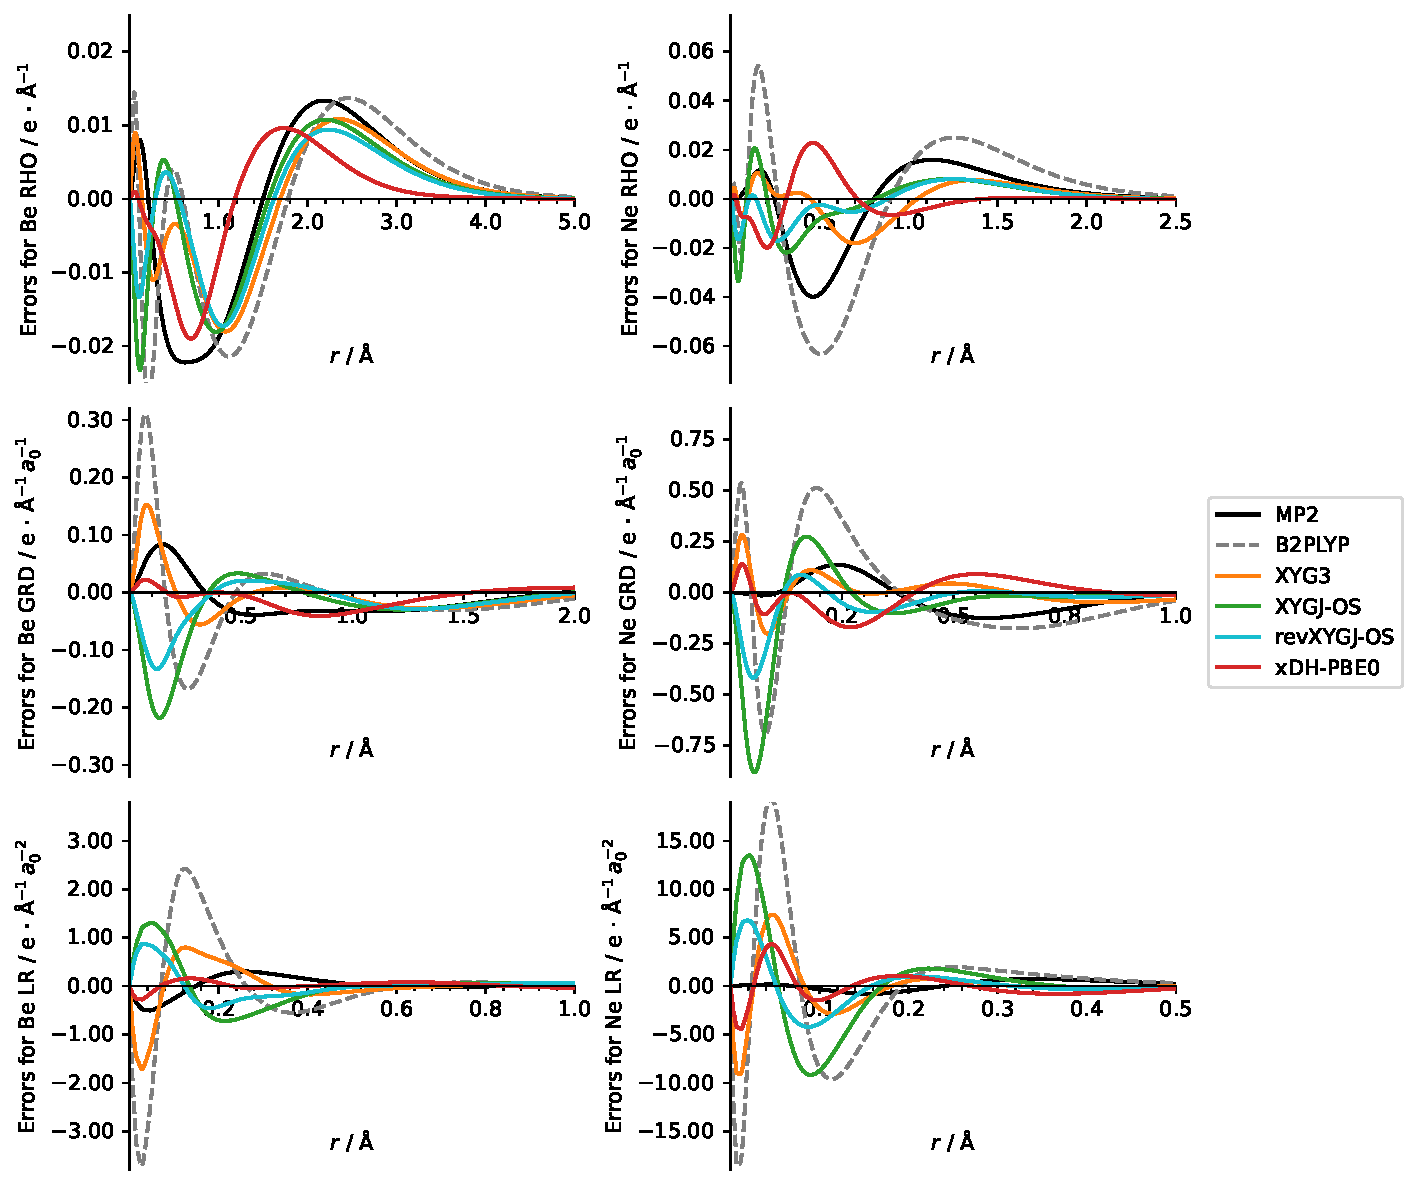
\includegraphics[width=0.95\textwidth]{assets/supp-fig-s1.pdf}
\end{figure}

\newpage

\begin{figure}[hp]
    \centering
    \caption{部分低阶泛函与 HF 方法的密度径向函数在 Be、Ne 原子上相对于 CCSD 方法的误差图。B3LYPV1R 指使用 VWN1RPA 作为 LDA 相关能部分的 B3LYP 方法。SVWN 的相关能部分是 VWN5。}
    \label{fig.supp-fig-s2}
    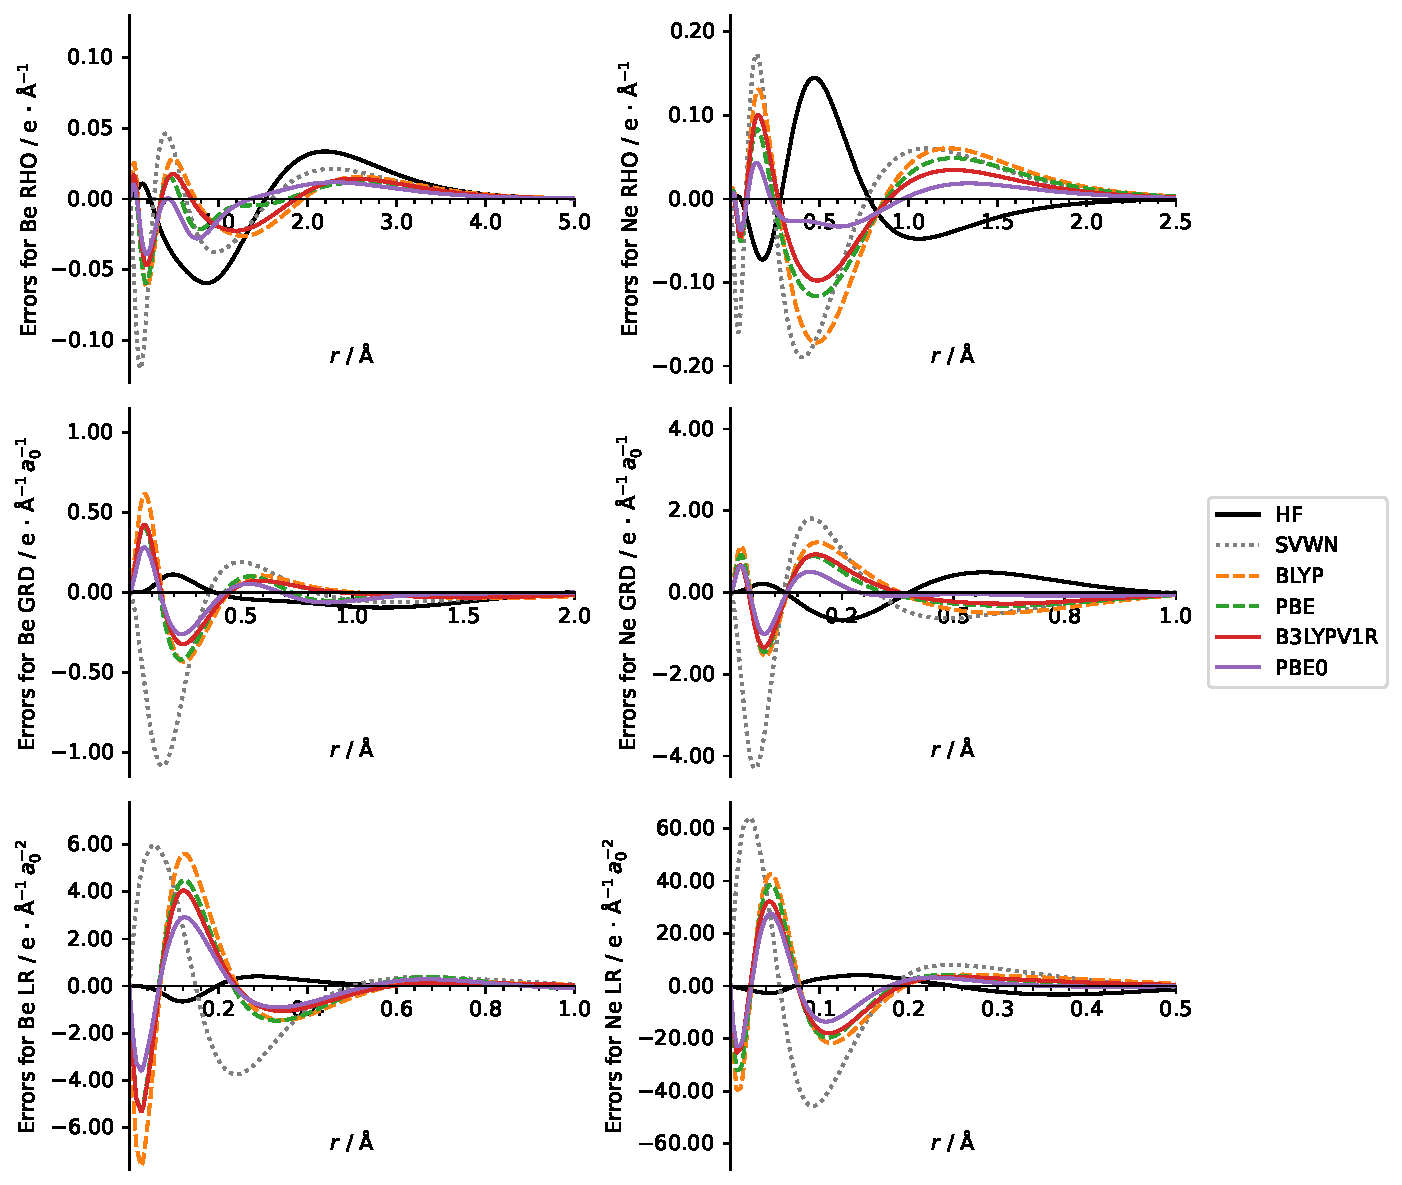
\includegraphics[width=0.95\textwidth]{assets/supp-fig-s2.pdf}
\end{figure}

\newpage

\begin{figure}[hp]
    \centering
    \caption{以 B3LYP 作为自洽场参考态的部分双杂化泛函 (XYG3, XYGJ-OS, revXYG3)、以及 B3LYP 的密度径向函数在 Be、Ne 原子上相对于 CCSD 方法的误差图。B3LYPV1R 指使用 VWN1RPA 作为 LDA 相关能部分的 B3LYP 方法,也是 XYG3 及其衍生泛函使用的自洽场参考态。}
    \label{fig.supp-fig-s3}
    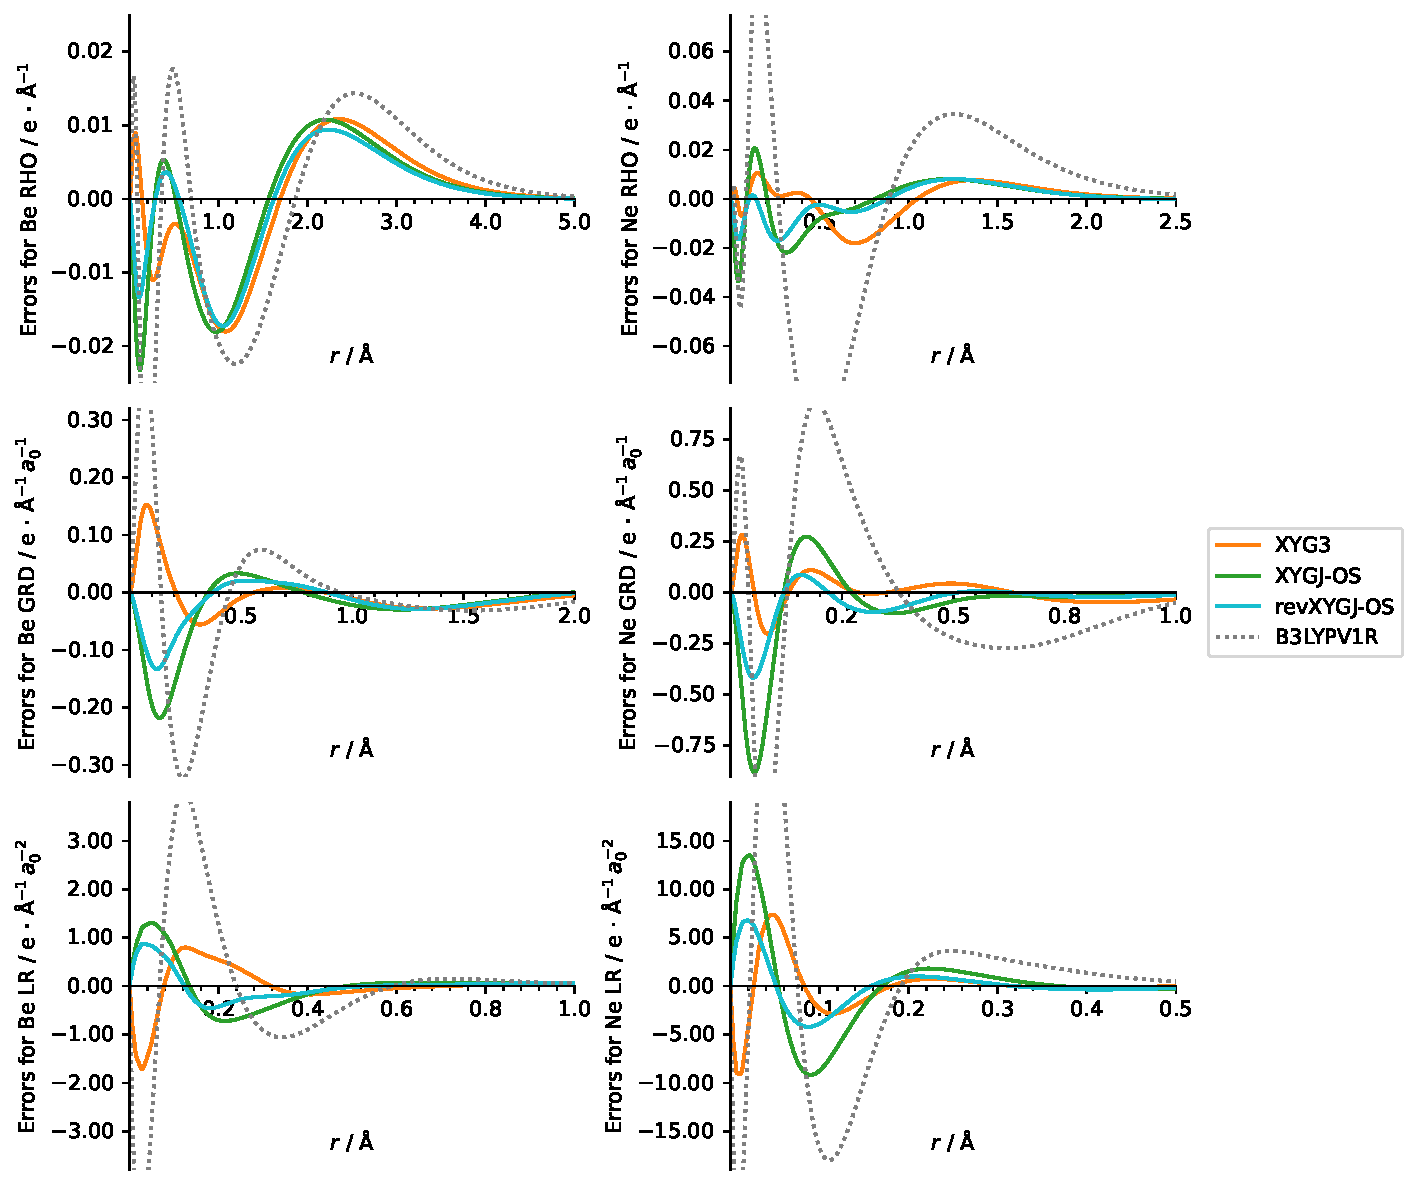
\includegraphics[width=0.95\textwidth]{assets/supp-fig-s3.pdf}
\end{figure}

\newpage

\begin{figure}[hp]
    \centering
    \caption{以 PBE0 作为自洽场参考态的部分双杂化泛函 (xDH-PBE0)、以及 PBE0 的密度径向函数在 Be、Ne 原子上相对于 CCSD 方法的误差图。}
    \label{fig.supp-fig-s4}
    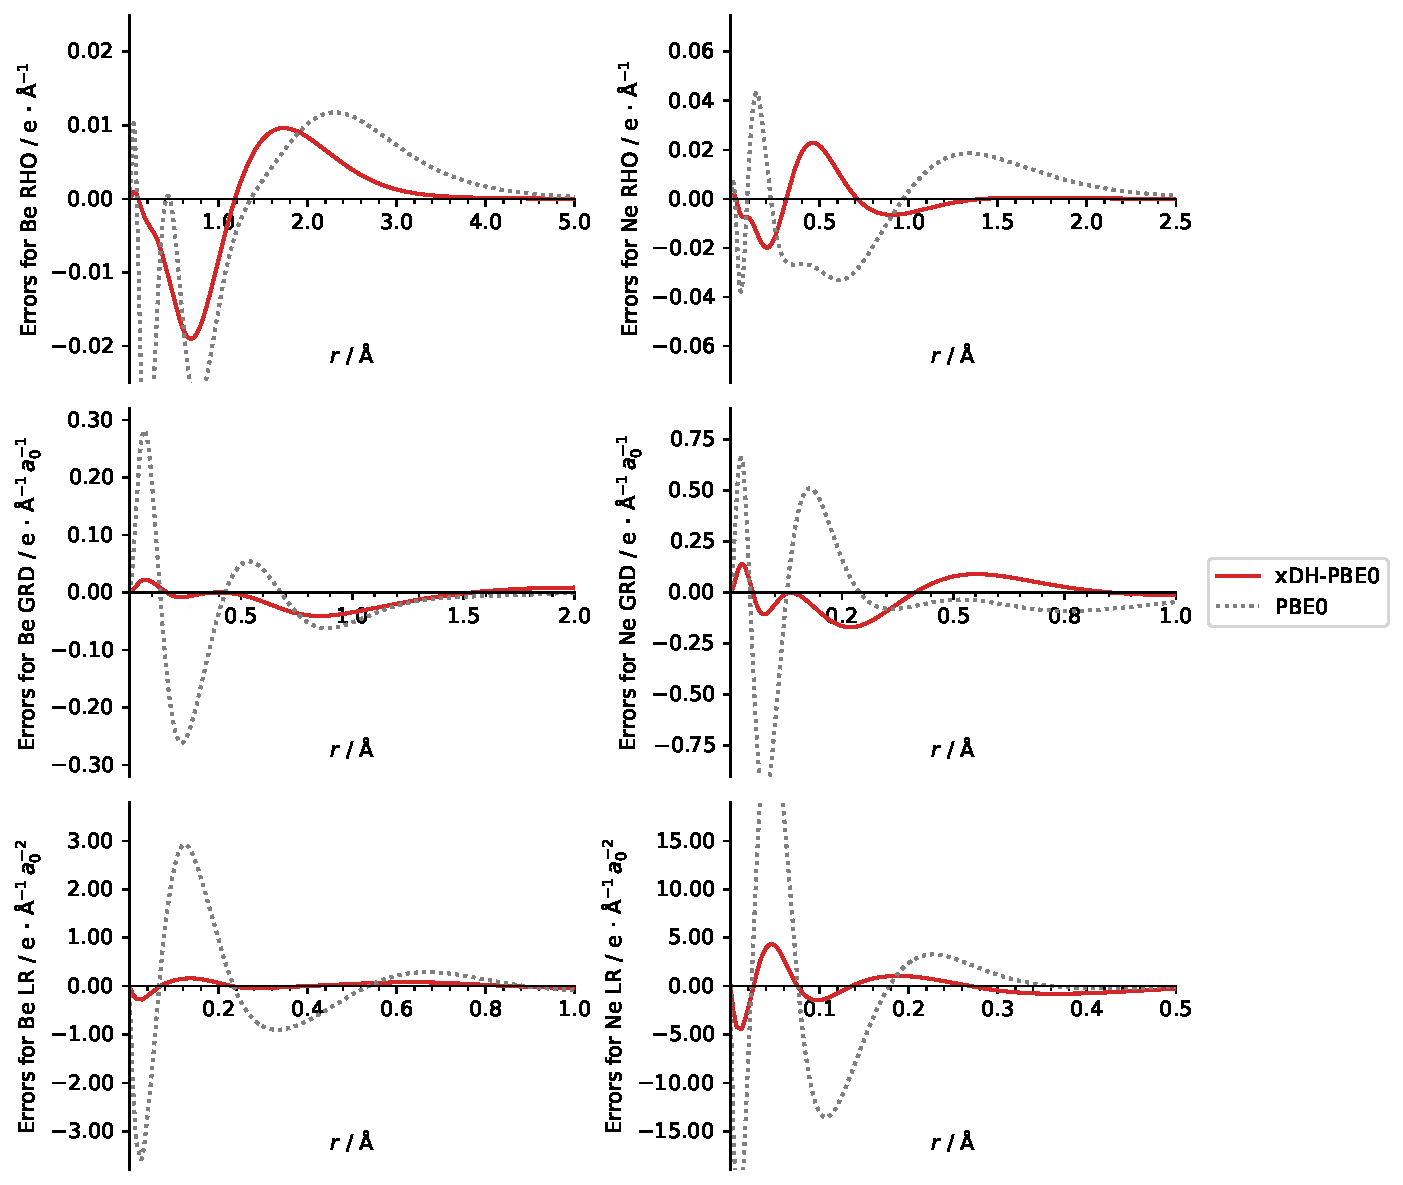
\includegraphics[width=0.95\textwidth]{assets/supp-fig-s4.pdf}
\end{figure}


\graphicspath{{../chap-05/}}
% !TEX root=./chap-05.tex
%-----全局定义-----
\documentclass[type=doctor]{fduthesis}
% \usepackage{fdudoc}

%-----FDU thesis setup-----
\fdusetup{
    style = {
        font = libertinus,
        cjk-font = founder,
        font-size = -4,
        fullwidth-stop = mapping,
        % footnote-style = xits,
        hyperlink = color,
        hyperlink-color = default,
        bib-backend = bibtex,
        bib-resource = {../thesis.bib},
        % bib-style = achemso,
        % cite-style = numerical,
        % declaration-page = {declaration.pdf},
        % 插入扫描版的声明页 PDF 文档
        % 默认使用预定义的声明页,但不带签名
        auto-make-cover = false,
        % 是否自动生成论文封面(封一)、指导小组成员名单(封二)和声明页(封三)
        % 除非特殊需要(e.g. 不要封面),否则不建议设为 false
    },
    %
    % info 类用于录入论文信息
    info = {
    title = {双杂化密度泛函分子能量与性质\\计算方法进展与测评},
    title* = {
        Recent Progress on Computational Method and Benchmark
        on Molecular Energy and Property of Doubly Hybrid Functional Approximations},
    % 英文标题
    %
    author = {祝震予},
    supervisor = {徐\quad 昕\quad 教授},
    major = {物理化学},
    degree = academic,
    department = {化学系},
    student-id = {17110220038},
    % date = {2023 年 1 月 1 日},
    % 日期
    % 注释掉表示使用编译日期
    instructors = {
        { 徐 昕    教 授 },
        { 张 颖    教 授 },
        { 段 赛   青年研究员},
        { 郑 晓    教 授 },
    },
    % 指导小组成员
    % 使用英文逗号 “,” 分隔
    % 如有需要,可以用 \quad 手工对齐
    %
    keywords = {密度泛函理论, 双杂化泛函, 电子云密度, 解析梯度性质, 静态极化率},
    % 中文关键词
    % 使用英文逗号 “,” 分隔
    %
    keywords* = {density functional theory, doubly hybrid functional, electron density, analytical derivative property, static polarizability},
    % 英文关键词
    % 使用英文逗号 “,” 分隔
    %
    clc = {O641.12},
    % 中图分类号
    }
}

%-----fduthesis issues-----
% issue #86
\ExplSyntaxOn
\tl_set:Nn \c__fdu_cover_info_align_tl { c @ { \c__fdu_fwid_colon_tl } l }
\ExplSyntaxOff
% 化学系图表格式要求
\ExplSyntaxOn
\cs_set:Npn \thefigure
{ \thechapter . \__fdu_arabic:n { figure } }
\cs_set:Npn \thetable
{ \thechapter . \__fdu_arabic:n { table } }
\ExplSyntaxOff

% expl3 在 tabulararray 包的冲突
% https://tex.stackexchange.com/a/463283
\usepackage{expl3}
\ExplSyntaxOn
\int_new:N \g__tblr_defined_hdash_styles_prop
\int_new:N \g__tblr_defined_vdash_styles_prop
\int_new:N \g__tblr_initial_rows_prop
\int_new:N \g__tblr_initial_columns_prop
\int_new:N \g__tblr_initial_table_prop
\int_new:N \g__tblr_initial_cells_prop
\int_new:N \g__tblr_initial_hlines_prop
\int_new:N \g__tblr_initial_vlines_prop
\ExplSyntaxOff

%-----图表设置-----
\usepackage{siunitx}
\usepackage{enumitem}
\newcommand{\tabnote}[1]{\textsuperscript{\emph{#1}}}
\usepackage{threeparttable}
\usepackage{threeparttablex}
\usepackage{graphicx}
\usepackage{longtable}
\usepackage{longfigure}
\usepackage{subcaption}
\usepackage{float}
\usepackage{lscape}
\usepackage{multicol}
\usepackage{multirow}
\usepackage{arydshln}
\usepackage{dcolumn}
\newcolumntype{d}[1]{D{.}{.}{#1}}
\setlength\dashlinedash{0.5pt}
\setlength\dashlinegap{1.5pt}
\setlength\arrayrulewidth{0.5pt}
\usepackage[figuresright]{rotating}
% \usepackage{booktabs}
\usepackage{tabularray}
\UseTblrLibrary{booktabs}
\usepackage{tcolorbox}

%-----化学符号-----
\usepackage[version=4]{mhchem}

%-----数学记号----
\usepackage[ntheorem]{empheq}
\allowdisplaybreaks[1]

%-----其它定义-----
\definecolor{msblue}{rgb}{0.05859375,0.28515625,0.43359375}
\definecolor{msorge}{rgb}{0.75390625,0.35156250,0.08593750}
\usepackage{ifthen}
\newcommand{\Schrodinger}{Schr\"o\-dinger}
\usepackage{tikz}
\usetikzlibrary{arrows.meta, graphs, shapes.misc, positioning}

% tablenotes 与表格内注释超链接 (from fdudoc.cls)
\makeatletter
\renewlist{tablenotes}{description}{1}
\setlist[tablenotes]{
  format      = \normalfont\itshape\tnote@item,
  labelwidth  = 0.5em,
  itemindent  = 0pt,
  rightmargin = \tabcolsep,
  leftmargin  = \the\dimexpr\tabcolsep+1em\relax,
  after       = \@noparlisttrue}
\AtBeginEnvironment{tablenotes}{%
  \setlength\parindent{2\ccwd}%
  \normalfont\footnotesize}
\AtBeginEnvironment{threeparttable}{%
  \stepcounter{tpt@id}%
  \edef\curr@tpt@id{tpt@\arabic{tpt@id}}}
\newcounter{tpt@id}
\def\tnote@item#1{%
  \Hy@raisedlink{\hyper@anchor{\curr@tpt@id-#1}}#1}
\def\TPTtagStyle#1{\textit{\hyperlink{\curr@tpt@id-#1}{#1}}}
\makeatother

% 用于表格注释与 threeparttable 环境引入的便利函数
\renewcommand{\TPTminimum}{\linewidth}
\newcommand{\widetabular}[2]{%
\ifx&#2&
  \begin{threeparttable}
    \centerline{\makebox[2\linewidth]{#1}}
  \end{threeparttable}
\else
  \begin{threeparttable}
    \centerline{\makebox[2\linewidth]{#1}}
  \begin{tablenotes}[nosep, topsep=0.5em]
    #2
  \end{tablenotes}
  \end{threeparttable}
\fi}

% 用于分章节编译与统稿的代码
\newcommand{\alert}[1]{{\color{red}{#1}}}
\newcommand{\alertref}[1]{{\color{red}{#1}}}
\newcommand{\alerthyperref}[2]{{\color{red}{#2}}}
\newcommand{\blindproof}[1]{{\color{blue}{#1}}}

% 用于表示方法的格式
\newcommand{\textmt}[1]{\textsf{#1}}

% 向量加粗的简记
\newcommand{\bm}{\symbfit}

% 保证 mathbb 被花括号包含
\renewcommand{\mathbb}[1]{{\symbb{#1}}}

%---------设定区结束----------

% 格式检查列表
% [ ] 表格数据使用 \widetabular{}{} 插入,以替代自定义的 \tabnote 和默认的 threeparttable。
% [ ] 表格 caption 在上,图片 caption 在下。图片不引入注释。
% [ ] 表格尽可能不引入纵向分割线。
% [ ] 建构术语表与符号表,避免文中出现术语定义、特别是英文定义。


\begin{document}

%---------预定设置区----------
\title{\textbf{双杂化密度泛函分子能量与性质计算方法的测评与进展\\第五章草稿}}
\author{祝震予}
\maketitle
\vspace{-10pt}

\tableofcontents

%---------正  文  区----------

\setcounter{section}{4}

\section{高精度基组外推方法在 CCSD(T) 静态极化率计算上的应用}

\subsection{引言}

静态极化率是光学中问题重要的物理量\cite{Marder-Stucky.ACS.1991};它在化学中,也与 Raman 光谱活性\cite{Wilson-Cross.Dover.1955}、有机反应机理\cite{Xing-Pei.HEP.2005}、以及分子间相互作用\cite{Cohen-Tannoudji-Laloe.Wiley.2020}等问题上有概念上的联系。作为计算化学可以导出的物理量,对静态极化率描述的准确与否,也可以用于判断电子结构近似方法精度与有效性。因此,静态极化率是理论与计算化学都十分关心的重要物理量。

相对于静态极化率的概念是动态极化率。动态极化率 $\alpha(\omega)$ 是在特定频率 $\omega$ 下偶极电场扰动下分子能量变化的表征量,而静态极化率是动态极化率的外场频率外推至零的情况即 $\alpha(0)$。本文中,若不作额外说明,极化率一般指静态极化率。

我们希望对双杂化泛函在静态极化率上的表现作评测与研究;为此,我们需要精确的静态极化率参考值。计算方法的终极目标应当是逼近物理真实的结果,因此参考值应当选取这些真实结果的数值;但现实上,真实结果难以获得。为了确定参考值以评测近似计算化学方法的有效性,可能的方案是以精确的实验数据、或高精度的计算数据替代参考值。

若要通过实验数据构成参考值以测评理论计算结果,一个关键问题与困难是如何准确地联系理论结果与实验环境\cite{Mata-Suhm.ACIE.2017}。对于静态极化率问题,我们认为,通过实验数据确定与获得参考值较为困难。这种困难不仅来源于实验本身的精度,也同时来源于难于排除所有实验环境因素;这些因素包括溶剂效应、非谐效应等各种影响,也因静态偶极矩是动态偶极矩在含频电场下频率外推至零的极限、实验上这种外推的矫正难于实现或精确的数据不足。因此,在目前的研究中,电子结构方法的误差经常会被实验本身的误差、以及实验环境与理论模拟之间的差距所产生的误差的总和所掩盖\cite{Hickey-Rowley.JPCA.2014}。因此,相比起使用实验数值作为参照的方式\cite{Hickey-Rowley.JPCA.2014},大多数对静态极化率的测评工作都使用高精度理论计算数值作为参考值\cite{Hammond-Xantheas.JCP.2009, Huzak-Deleuze.JCP.2013, Wu-Thakkar.CPL.2015, Kozlowska-Bartkowiak.PCCP.2019, Hait-Head-Gordon.PCCP.2018, Beizaei-Sauer.JPCA.2021}。

若要使用理论参考值作测评工作,有两点非常关键。一者,为了确保评测相对来说公平且完整,数据集应当要足够大、且足够多样,以使得在测评结果在统计上是有意义的。目前的极化率数据集中,较为接近这一目标的有 Hickey 与 Rowley 设计的 46 分子的数据集 (HR46)\cite{Hickey-Rowley.JPCA.2014},Wu、Kalugina 与 Thakkar 设计的 145 分子数据集 (T145)\cite{Wu-Thakkar.CPL.2015}、以及 Hait 与 Head-Gordon 设计的 132 分子与自由基数据集 (HH132)\cite{Hait-Head-Gordon.PCCP.2018}。二者,作为参考值的电子结构理论计算方法应当足够准确。完全组态相互作用 (Full-CI, Full-\underline{C}onfiguration-\underline{I}nteraction) 结合完备基组 (CBS, \underline{C}omplete \underline{B}asis \underline{S}et) 所给出的结果是最理想的情况,但其计算量巨大,显然是不现实的。HH132 数据集选择使用 CCSD(T)/CBS,即化学中常称为“黄金标准”的 CCSD(T) 方法 (\underline{C}oupled-\underline{C}luster \underline{S}ingles and \underline{D}oubles with perturbative \underline{T}riples)\cite{Cizek-Cizek.Wiley.1969, Raghavachari-Head-Gordon.CPL.1989}、并结合有限基组下的 CBS 外推方法\cite{Nyden-Petersson.JCP.1981, Petersson-Mantzaris.JCP.1988},给出了极化率的参考值。其中,对于较小的体系,用于 CBS 外推的模式是 aCV[Q5]Z\footnote{在本文中,我们约定作为 Dunning 系列基组的 aV$X$Z 代表 aug-cc-pV$XZ$ 基组、aCV$X$Z 代表 aug-cc-pCV$XZ$ 基组 ($X \in \{\mathrm{D, T, Q, 5}\}$)。同时约定,作为双基组 CBS 外推模式,aV[$XY$]Z 代表基组从 aV$X$Z、aV$Y$Z 外推到 aV$\inf$Z 的基组极限近似。本工作中,Dunning 系列基组具体的 CBS 外推方式定义于式 (\ref{eq.cbs.zeta3})。};对于较大的体系,用于 CBS 外推的模式是 aCV[TQ]Z\cite{Hait-Head-Gordon.PCCP.2018, Hait-Head-Gordon.JCTC.2018}。由于 CBS 外推所用的基组,几乎已是目前计算化学常用的最大基组。对于 CCSD(T) 在电性质计算问题上的准确性,已有文献对此作较为深入的讨论并给出正面的结论\cite{Halkier-Joergensen.JCP.1999, Monten-Deleuze.MP.2011, Hait-Head-Gordon.JCTC.2018}。因此,HH132 数据集的参考值可以认为是可信的。与此同时,HR46 数据集中理论计算给出参考值的模型是 CCSD/aVTZ,而 T145 数据集是 CCSD(T)/aVTZ;CCSD 被认为在计算电性质时精度较低、而 aVTZ 基组也相对较小,因此这两个数据集的理论计算参考值相对于 HH132 数据集,还有进一步提升的空间。

但需要指出,HH132 之所以可以使用 CCSD(T)/aV[TQ]Z 或 CCSD(T)/aV[Q5]Z 的模型给出参考值,是因为该数据集最大的分子仅包含 3 个非氢原子 (包括 \ce{BHF2}, \ce{ClCN}, \ce{CO2}, \ce{CSO}, \ce{FCN}, \ce{FCO}, \ce{HCCCl}, \ce{HCCF}, \ce{HCNH2}, \ce{HCOOH}, \ce{NaCN}, \ce{NOCl}, \ce{O3}, \ce{OCl2}, \ce{OF2}, \ce{SCl2}, \ce{SF2}, \ce{SO2})、或 7 个原子 (包括 \ce{CH3NH2})。而作为对比,HR46 与 T145 数据集的分子相对来说大许多;HR46 最大的体系包含 15 个原子 (toluene 或 \ce{C7H8});T145 数据集最大的体系包含 14 个原子 (1,4-dithiane 或 \ce{C4H8S2})。HR46 与 T145 数据集中,单个体系含有非氢原子数量最多可达 8 个原子 (例如 6-amino-1H-pyrimidin-2-one 或 \ce{C4H5ON3} 以及 5,5,5-trichloropenta-1,3-diyne 或 \ce{C5HCl3})。因此,HR46 与 T145 数据集难以使用与 HH132 相同的 CCSD(T) 结合大基组 CBS 外推的方式,给出精确地理论计算的参考值。

为了尽可能地推高 HR46 与 T145 数据集的精度,我们考虑到使用组合化学方法。典型的组合化学方法是 G$n$\cite{Pople-Curtiss.JCP.1989, Curtiss-Pople.JCP.1990, Curtiss-Pople.JCP.1991, Curtiss-Pople.JCP.1998, Curtiss-Raghavachari.JCP.2007} 与 W$n$\cite{Martin-Oliveira.JCP.1999, Parthiban-Martin.JCP.2001};其做法是针对特定的电子结构方法 (如 CCSD(T), CCSD, MP2, HF),使用对应的、代价上可以承受的基组进行计算,并最终合理地依计算层级对这些方法-基组组合的结果作线性的加减处理,给出更为精确地计算结果。FPA (\underline{F}ocal-\underline{P}oint \underline{A}nalysis) 与组合化学方法有着类似的思想\cite{East-Allen.JCP.1993}。由于能量或极化率张量等性质具有可加性,因此可以将总量上占大头的 HF 方法下大基组计算的结果、MP2 与 HF 方法差减部分在中等基组下计算结果、以及计算复杂度最高但总量上较小的 CCSD(T) 与 MP2 方法差减部分在较小基组下的计算结果作加和。这样的结果一般总是比单纯使用低级别的 HF 结合大基组、或高级别的 CCSD(T) 结合小基组要更为准确。FPA 已经应用于计算化学的各种问题,包括反应生成热\cite{East-Allen.JCP.1993, Nielsen-Schaefer.JCP.1997}、构象能\cite{Csaszar-Schaefer.JCP.1998, Tschumper-Tschumper.JCP.2001, Kahn-Kahn.JCC.2008}、非共价相互作用\cite{Tschumper-Quack.JCP.2002, Jurecka-Hobza.PCCP.2006, Marshall-Sherrill.JCP.2011}、激发能\cite{Bokareva-Godunov.IJQC.2008}、核磁共振屏蔽常数\cite{Sun-Xu.JCP.2013, Wang-Xu.JCP.2018}、以及本工作所关心的静态极化率问题\cite{Huzak-Deleuze.JCP.2013, Monten-Deleuze.MP.2011}。

本工作中,我们将着眼于提升 HR46 与 T145 静态极化率数据集的质量至 CCSD(T)/CBS 的精度。为此,我们首先在可以承受 aCV[Q5]Z 级别计算的小分子体系下,对 HF, MP2, CCSD 与 CCSD(T) 作详细的静态极化率基组收敛性分析。这部分工作的目标是确认对于静态极化率问题,FPA 确实可以给出与 HH132 数据集参考值相似精度的结果,即 FPA 是有效的。随后,我们将 FPA 应用于 HR46 与 T145 数据集的参考值计算上;这些参考值的精度将是 CCSD(T)/aCV[Q5]Z 级别的。我们希望这些高精度的参考值能为未来化学工作者在极化率测评,特别是对密度泛函方法的测评上,提供有效的数据来源。

\subsection{具体方法与实现细节}

\subsubsection{误差测评标准}

对于一个数据量为 $N$ 的数据集的参考值是 $\tilde r = \{ r_n \}$,若近似计算方法的结果是 $\tilde c = \{ c_n \}$、以及作为分母的数据 $\tilde d = \{ d_n \}$,那么数据 $\tilde c$ 的相对方均根误差 (RelRMSD, \underline{Rel}ative \underline{R}oot \underline{M}ean \underline{S}quared \underline{D}eviation) 定义为
\begin{equation}
    \text{RelRMSD} (\tilde c, \tilde r, \tilde d) = \sqrt{\frac{1}{N} \sum_{n = 1}^N \left( \frac{c_n - r_n}{d_n} \right)^2} \times 100\%
\end{equation}
不少情况下,参考值 $\tilde r$ 与分母值 $\tilde d$ 是相同的;此情形下将简记 $\text{RelRMSD} (\tilde c, \tilde r, \tilde d)$ 为 $\text{RelRMSD} (\tilde c, \tilde r)$。一般来说,更低的 RelRMSD 数值,意味着近似计算方法的表现统计上来看越精确。

RelRMSD 误差多大,才认为是可以被接受或容许的范围?首先,本工作的目标是对较大分子体系的极化率作逼近 CBS 外推模型的 CCSD(T)/aCV[Q5]Z 精度的计算;因此,该级别精度在本工作中视为最精确的参考值 $\tilde r$。由于静态极化率的基组极限误差与实验误差通常在 0.5\% 以内\cite{Brakestad-Frediani.JCTC.2020, Rumble-Rumble.CRC.2021};因此我们认为,对于稍低等级的 FPA 模型或稍小基组下的计算结果,如果其相比于 CCSD(T)/aCV[Q5]Z 的 RelRMSD 误差在 0.5\% 以下,即可认为是足够准确的。

% 关于实验误差,我暂时没能找到 102 版 CRC 常数手册的具体说明。在 2010 年的 90 版 Atomic and Molecular Polarizabilities Table 8 (pdf p. 1648--1649 或 10-200--10-201),注脚中提到了 0.5% 的误差,但也同时指出了实验条件上是含频率的情况、以及数据年代问题。

\subsubsection{电子结构方法与软件}

本工作的极化率同时使用数值与解析的方式计算。MP2 与 HF 解析极化率是通过 \textsc{PySCF} (commit 3d592b0)\cite{Sun-Chan.WCMS.2018, Sun-Chan.JCP.2020}的扩展程序脚本 \textsc{dh} (ver 0.1.3)\cite{dh-0.1.ajz34} 所实现。正因为该程序可以高效地实现包括双杂化泛函在内的 MP2 型相关能解析极化率,因此本工作中涉及到的所有分子的 MP2 极化率,在引入 RI 近似的前提下,都可以以最精确的 CBS 外推模式 aCV[Q5]Z 实现。对于 CCSD 与 CCSD(T) 方法,本工作使用 \textsc{Q-Chem} (ver 5.1.1)\cite{Shao-Head-Gordon.MP.2015, Kaliman-Krylov.JCC.2017}作数值极化率计算。这部分计算将不引入 RI 近似。本工作不对 post-HF 计算过程引入冻核近似 (FC, \underline{F}rozen \underline{C}ore)。自由基与其他开壳层体系的 HF 自洽场参考态通过自旋非限制性计算给出。

本工作将在 \ref{sec.5.3.1} 小节对极化率的数值与解析之间的误差、RI 近似所导致的误差、以及基组误差进行分析。最终汇报的极化率数值中,HF 与 MP2 是通过 RI 近似下解析给出 (这两个方法将分别记为 RI-JK 与 RI-MP2);CCSD 与 CCSD(T) 的结果将是 RI-MP2 解析极化率、以及更高阶贡献的数值极化率的加和。为更清晰明了地表示极化率数值的构成,本文将使用简记记号;这些记号列于表 \ref{tab.5.1}。该表格的所有记号是针对单个分子或自由基体系的;对于一个数据集合,我们将上标波浪号。举例而言,$\text{RelRMSD} (\Delta \tilde \alpha_{\textsf{(2)}/\text{aVTZ}}, \Delta \tilde \alpha_{\textsf{(2)}/\text{ref}}, \tilde \alpha_{\textsf{CCSD(T)}/\text{ref}})$ 代表 MP2/aVTZ 同性极化率相对于高精度 MP2 参考值的相对方均根误差;该相对误差计算所用的分母,是高精度 CCSD(T) 参考值。

\begin{table}[ht]
    \centering
    \caption{本工作中使用的电子结构方法及其对应极化率的记号\tabnote{a}。}
    \label{tab.5.1}
    \begin{tabular}{ll}
    \hline
    记号 & 说明 \\
    \hline
    num & 数值极化率 \\
    anal & 解析极化率 \\
    conv & 传统电子积分方法,即无 RI 近似的计算方法 \\
    $\alpha$ & 同性极化率 \\
    $\gamma$ & 异性极化率 \\
    $\Delta \alpha_\textsf{(2)}$ & $\alpha^\text{anal}_\textsf{RI-MP2} - \alpha^\text{anal}_\textsf{RI-HF}$ \\
    $\Delta \alpha_\textsf{D}$ & $\alpha^\text{num}_\textsf{CCSD} - \alpha^\text{num}_\textsf{MP2}$ (不引入 RI 近似) \\
    $\Delta \alpha_\textsf{(T)}$ & $\alpha^\text{num}_\textsf{CCSD(T)} - \alpha^\text{num}_\textsf{CCSD}$ (不引入 RI 近似) \\
    $\Delta \alpha_\textsf{D(T)}$ & $\alpha^\text{num}_\textsf{CCSD(T)} - \alpha^\text{num}_\textsf{MP2}$ (不引入 RI 近似) \\
    $\Delta \alpha_\textsf{HF}$ & $\alpha^\text{anal}_\textsf{RI-HF}$ \\
    $\Delta \alpha_\textsf{MP2}$ & $\alpha^\text{anal}_\textsf{RI-MP2} = \alpha_\textsf{HF} + \Delta \alpha_\textsf{(2)}$ \\
    $\alpha_\textsf{CCSD}$ & $\alpha^\text{num}_\textsf{CCSD} - \alpha^\text{num}_\textsf{MP2} + \alpha^\text{anal}_\textsf{RI-MP2} = \alpha_\textsf{HF} + \Delta \alpha_\textsf{(2)} + \Delta \alpha_\textsf{D}$ \\
    $\alpha_\textsf{CCSD(T)}$ & $\alpha^\text{num}_\textsf{CCSD(T)} - \alpha^\text{num}_\textsf{MP2} + \alpha^\text{anal}_\textsf{RI-MP2} = \alpha_\textsf{HF} + \Delta \alpha_\textsf{(2)} + \Delta \alpha_\textsf{D(T)}$ \\
    \hline
    \end{tabular}
  
    \raggedright
    \par\tabnote{a} 上述所有应用于同性极化率 $\alpha$ 的记号,将同样应用于异性极化率 $\gamma$。
\end{table}

\subsubsection{数据集}

本工作着重考察的数据集是 HR46 与 T144。原始的 HR46 数据集\cite{Hickey-Rowley.JPCA.2014}包含 46 个体系 (化合物结构参考附录图 \ref{fig.fig-s1});其最精确的计算模型是在 MP2/aVTZ 结构下 CCSD/aVTZ 极化率,且该工作中使用了冻核近似。该数据集的特点是
\begin{itemize}[nosep]
    \item 包含的原子种类较多,包括 H, C, N, O, F, S, P, Cl, Br 等元素;
    \item 在 15 个原子以内的限制下,包含大多数常见有机官能团与无机共价键或离域键;
    \item 分子或自由基的选取契合化学反应、污染控制、生物化学与能源化学的需求;
    \item 除了 3 个体系是自由基体系 (\ce{^2NO}, \ce{^3O2}, \ce{^3SO},上标的数字表示自旋多重度),其余体系均为非自旋极化的体系 (non-spin-polarized)。
\end{itemize}
在本工作中,HR46 中的所有分子的几何结构经过 RI-MP2/aVTZ 级别作优化,且没有启用冻核近似\alert{盲审通过后将结构的链接链上}。所有极化率的计算也在此几何结构下实现。

原始的 T145 数据集\cite{Wu-Thakkar.CPL.2015}包含 145 个有机体系。该数据集的分子使用 B3LYP/aVTZ 下的优化结构,最精确的极化率计算模型是 CCSD(T)/aVTZ。T145 数据集是 TABS 数据集\cite{Blair-Thakkar.CTC.2014}的子集。TABS 数据集本身是一大类着眼于药物化学、有机化学与生物化学应用的、自旋非极化的数据集。TABS 数据集的分子数量为 1641;一方面该数据集本身数量较大、另一方面为使该数据集用于机器学习,Blair 等人对 TABS 挑选 298 分子作为极化率与分子容量的训练集为 T298 数据集\cite{Blair-Thakkar.CPL.2014}。但由于并非所有 T298 数据集中的分子都可以承受 CCSD(T)/aVTZ 的计算代价,因此 Wu 等人从 T298 选出 145 个较小的分子,以给出极化率参考值更精确的数据集,即 T145 数据集\cite{Wu-Thakkar.CPL.2015}。本工作中,我们选取其中的 144 个分子,并称其为 T144 数据集。相比于 T145 数据集,我们排除了第 1363 号分子 (TABS 分子编号,分子名称为 2,3-dihydro-1,3-oxazole);这是因为 TABS 数据集提供的分子构型中,1363 号分子与分子式对应的结构相差两个氢原子,即可能存在数据的损坏。T144 数据集的分子构型使用 TABS 原始数据库提供的 B3LYP/aVTZ 几何结构\cite{Blair-Thakkar.CTC.2014} (化合物结构参考附录图 \ref{fig.fig-s2-1})。

关于 HR46 与 T144 数据集化合物名称的变化与勘定,参考附录 \ref{sec.T145-HR46-name-change}。

本工作的一个关键点是基组收敛性评测。为作有效的评测,测评的体系应可承受高精度大基组 (如 CCSD(T)/aCV5Z 级别模型) 的计算量与资源需求。在 HR46 与 T144 数据集中,14 个体系 (\ce{Cl2}, \ce{CO}, \ce{CO2}, \ce{H2O}, \ce{N2}, \ce{NH3}, \ce{^3O2}, \ce{PH3}, \ce{SH2}, \ce{SiH4}, \ce{^3SO}, \ce{SO2}, \ce{FCN}, \ce{HCHS}) 可以承受大计算量的计算。这 14 个数据也同样出现在 HH132 数据集中。在测评基组收敛性问题时,这 14 个小体系的分子构型将采用 NIST 计算化学数据库中实验的数据\cite{NIST.CCCBDB};这些构型也同样为 HH132 数据集所采用。

\subsubsection{基组与 RI 近似}

在本工作中,我们将使用 Dunning 系列基组 aV$X$Z 与 aCV$X$Z ($X = \mathrm{D, T, Q, 5}$)\cite{Dunning-Dunning.JCP.1989, Kendall-Harrison.JCP.1992, Woon-Dunning.JCP.1993, Peterson-Dunning.JCP.1994, Wilson-Dunning.JMST.1996, VanMourik-Dunning.MP.1999, Wilson-Dunning.JCP.1999, VanMourik-Dunning.IJQC.2000, Peterson-Dunning.JCP.2002, Hill-Peterson.JCP.2010}。H 与 Br 原子并不出现在 aCV$X$Z 系列基组中;对于这两个原子作 aCV$X$Z 级别计算时,将不加说明地替换为对应的 aV$X$Z 基组。RI 近似可以大幅减少 MP2 的计算耗时,并且不会产生严重的误差损耗,是性价比相当高的技术手段\cite{Vahtras-Feyereisen.CPL.1993}。本工作的解析极化率计算中,我们对 Weigend 算法实现的 RI-JK\cite{Weigend-Weigend.PCCP.2002} 与 RI-MP2 相关贡献\cite{Weigend-Haettig.JCP.2002}计算均使用等比辅助基 (ETB, \underline{E}ven-\underline{T}empered auxiliary \underline{B}asis set)\cite{Stoychev-Neese.JCTC.2017};等比参数设为 \textsc{PySCF} 程序默认的 $\beta = 2$。由于基于 \textsc{PySCF} 的扩展程序 \textsc{dh} 的高效率实现、以及对大基组下内存的合理控制,使得本工作中所有体系都可以在 MP2/aCV5Z 下完成计算。作为自洽场的 RI-JK 方法的能量收敛精度为 $10^{-10}$ Hartree。

\subsubsection{数值极化率}

在\alert{第三章的讨论}中,我们已经了解极化率是对外电场强度的二阶梯度;依外电场 $\pmb{\mathcal{E}}$ 在三个空间方向取向的大小 $(\mathcal{E}_x, \mathcal{E}_y, \mathcal{E}_z)$,极化率张量 $\bm{\alpha}$ 是 $3 \times 3$ 的对称矩阵:
\begin{equation}
    \alpha_{ts} = - \frac{\partial^2 E}{\partial \mathcal{E}_t \partial \mathcal{E}_s} \quad t, s \in \{ x, y, z \}
\end{equation}
作为物理上可观测的量,本工作着重测评同性极化率 $\alpha$\footnote{通过标量记号表示,用以区分作为矩阵的极化率张量 $\bm{\alpha}$。}和异性极化率 $\gamma$:
\begin{align}
    \alpha &= \frac{1}{3} \left( \alpha_{xx} + \alpha_{yy} + \alpha_zz \right) = \mathrm{tr} (\bm{\alpha}) \\
    \gamma &= \frac{1}{\sqrt{2}} \left( (\alpha_{xx} - \alpha_{yy})^2 + (\alpha_{yy} - \alpha_{zz})^2 + (\alpha_{zz} - \alpha_{xx})^2 + 6 (\alpha_{xy}^2 + \alpha_{yz}^2 + \alpha_{zx}^2) \right)^{1/2}
\end{align}
对于数值极化率的求取过程,对角元部分 $\alpha_{tt}$ ($t \in \{ x, y, z \}$) 通过线性的三点格式作数值导数给出:
\begin{equation}
    \label{eq.pol-findiff-alpha-def}
    \alpha_{tt} = - \frac{\partial^2 E}{\partial \mathcal{E}_t^2} = - \frac{1}{h^2} \left( E(- \bm{h}_t) - 2 E(\bm{0}) + E(\bm{h}_t) \right) + o(h^2)
\end{equation}
而非对角元部分 $\alpha_{ts}$ ($t, s \in \{ x, y, z \}, \, t \neq s$) 则通过平面上的三点格式作数值导数给出:
\begin{equation}
    \label{eq.pol-findiff-gamma-def}
    \alpha_{ts} = - \frac{\partial^2 E}{\partial \mathcal{E}_t \partial \mathcal{E}_s} = - \frac{1}{4h^2} \left( E(- \bm{h}_t - \bm{h}_s) - E(- \bm{h}_t + \bm{h}_s) - E(\bm{h}_t - \bm{h}_s) + E(\bm{h}_t + \bm{h}_s) \right) + o(h^2)
\end{equation}
其中,$\bm{h}_t, \bm{h}_s$ 分别是 $t, s$ 方向外加微扰电场强度矢量:
\begin{equation*}
    \bm{h}_x = (h, 0, 0)^\dagger, \quad \bm{h}_y = (0, h, 0)^\dagger, \quad \bm{h}_z = (0, 0, h)^\dagger
\end{equation*}
标量 $h$ 是微扰电场的强度;在本工作的数值差分计算中,我们对所有体系均使用 $h = 0.004$ au。关于使用该外加微扰强度的合理性,我们在附录的 \ref{sec.5.s9} 小节中作讨论。

数值梯度计算大多数情形使用 \textsc{Q-Chem} 程序。自洽场的收敛判据 (\texttt{SCF\_CONVERGENCE} 关键词) 设为 $10^{-11}$ au,而 CCSD 能量与振幅收敛判据 (\texttt{CC\_E\_CONV} 与 \texttt{CC\_T\_CONV}) 分别设为 $10^{-10}$ au 与 $10^{-7}$ au。作为特例,对于 \ce{^2NO} 分子,其数值梯度是通过 \textsc{PySCF} 在限制分子对称性的不可约表示而实现;其自洽场与 CCSD 收敛判据与 \textsc{Q-Chem} 设置相同。由于我们在以 aCV5Z 基组计算 \ce{SO2} 分子时遇到收敛困难,因此该情形下我们分别降低 \textsc{Q-Chem} 的收敛判据 \texttt{SCF\_CONVERGENCE}, \texttt{CC\_E\_CONV}, \texttt{CC\_T\_CONV} 为 $10^{-10}$ au, $10^{-9}$ au, $10^{-6}$ au。

\subsubsection{CBS 外推}

CBS 外推方法通常被认为在计算资源不足、以及有限基组不充分大时,可以有效地提升计算精度以更接近完备基组极限的手段。关于具体的 CBS 外推方法与策略,目前已有许多文献对此作说明与讨论\cite{Nyden-Petersson.JCP.1981, Petersson-Mantzaris.JCP.1988, Dunning-Dunning.JCP.1989, Peterson-Dunning.JCP.1994, Jensen-Jensen.TCA.2005, Karton-Martin.TCA.2006, Truhlar-Truhlar.CPL.1998, Klopper-Kutzelnigg.JMST.1986, Kutzelnigg-Morgan.JCP.1992, Martin-Martin.CPL.1996, Helgaker-Noga.JCP.1997, Halkier-Wilson.CPL.1998, Halkier-Olsen.CPL.1999}。HH132 数据集的原始工作使用的 CBS 策略是三次外推式\cite{Hait-Head-Gordon.PCCP.2018}
\begin{equation}
    \label{eq.cbs.zeta3}
    \alpha(\zeta) = \alpha(\text{CBS}) + A \zeta^{-3}
\end{equation}
其中,$\zeta$ 是基组的基数 (cardinal number)。对于 Dunning 基组,aV$X$Z 或 aCV$X$Z 的 $X = \mathrm{D, T, Q, 5}$ 分别对应的基数是 $\zeta = 2, 3, 4, 5$。对于 CBS 外推模型 aCV[TQ]Z,其相对于 aCV5Z 的误差,对于偶极矩大约是 $\sim 0.2\%$\cite{Hait-Head-Gordon.JCTC.2018, Halkier-Joergensen.JCP.1999},对于极化率大约是 $\sim 0.1\%$\cite{Hait-Head-Gordon.PCCP.2018};这意味着三次外推式 (\ref{eq.cbs.zeta3}) 对电性质的计算是有效的。在本工作中,对极化率的计算将沿用该 CBS 外推策略。对于 HR46 与 T144 全部分子的 MP2 极化率的计算,我们都使用 aCV[Q5]Z 作为参考值;而对于 CCSD 与 CCSD(T) 计算,则会依照分子体系的大小而给予相适应的 CBS 外推模型 aV[$XY$]Z ($[XY] = \mathrm{[Q5], [TQ], [DT]}$) 计算。

\subsubsection{FPA 策略}

在有限的计算资源内,若高等级方法难以直接计算得到,那么 FPA 方法会是一种尽可能逼近高等级计算方法结果、但使用相对较小计算资源的手段。在本工作中,我们的目标是给出 CCSD(T)/CBS 的参考值,其中的 CBS 是通过高精度的 aCV[Q5]Z 外推近似得到。考虑到不是所有体系都可以承受如此大的计算量,因此对极化率作三部分拆分:以同性极化率为例,CCSD(T) 极化率 $\alpha_\textsf{CCSD(T)}$ 拆分出这三部分是 HF 部分 $\alpha_\textsf{HF}$、MP2 相关贡献部分 $\Delta \alpha_\textsf{(2)}$、以及更高阶贡献部分 $\Delta \alpha_\textsf{D(T)}$:
\begin{align}
    \alpha_{\textsf{CCSD(T)}/\text{CBS}} &= \alpha_{\textsf{HF}/\text{CBS}} + \Delta \alpha_{\textsf{(2)}/\text{CBS}} + \Delta \alpha_{\textsf{D(T)}/\text{CBS}} \notag\\
    &\simeq \alpha_{\textsf{HF}/\text{LB}} + \Delta \alpha_{\textsf{(2)}/\text{CBS}} + \Delta \alpha_{\textsf{D(T)}/\text{CBS}'} \notag\\
    &\simeq \alpha_{\textsf{HF}/\text{LB}} + \Delta \alpha_{\textsf{(2)}/\text{CBS}} + \Delta \alpha_{\textsf{D(T)}/\text{SB}}
\end{align}
上式下标的 LB 是指大基组 (\underline{L}arge \underline{B}asis set)、SB 是指小基组 (\underline{S}mall \underline{B}asis set)。我们的工作对 HF 方法直接采用 $\text{LB} = \text{aCV5Z}$ 基组。对于 MP2 的相关贡献部分 $\Delta \alpha_{\textsf{(2)}/\text{CBS}}$,我们始终选择使用最高精度的 aCV[Q5]Z 外推模型。更高阶贡献部分 $\Delta \alpha_{\textsf{D(T)}/\text{CBS}'}$ 是指对高精度 CBS 外推 $\Delta \alpha_{\textsf{D(T)}/\text{CBS}}$ 的近似;目前针对 $\Delta \alpha_{\textsf{D(T)}/\text{CBS}'}$ 的计算基组级别取决于体系的大小。若对 $\Delta \alpha_{\textsf{D(T)}/\text{CBS}'}$ 的计算使用基组 aV[$XY$]Z 与 aCV[$XY$]Z,那么我们称该 FPA 策略为 FPA-aV[$XY$]Z。同样地,若对 $\Delta \alpha_{\textsf{D(T)}/\text{LB}}$ 的计算使用基组 aV[$X$]Z 与 aCV[$X$]Z ($X < 5$),那么我们称该 FPA 策略为 FPA-aV[$X$]Z。

\begin{figure}[ht]
    \centering
    \caption{本工作所使用的 FPA 模型。该图以 FPA-aV[TQ]Z 作为例子;其中 $\alpha_{\textsf{HF}/\text{LB}}$ 以 aCV5Z 计算所得、$\Delta \alpha_{\textsf{(2)}/\text{CBS}}$ 以 aCV[Q5]Z 计算所得、$\Delta \alpha_{\textsf{D(T)}/\text{CBS}'}$ 以 aV[TQ]Z 计算所得。}
    \label{fig.fig-1}
    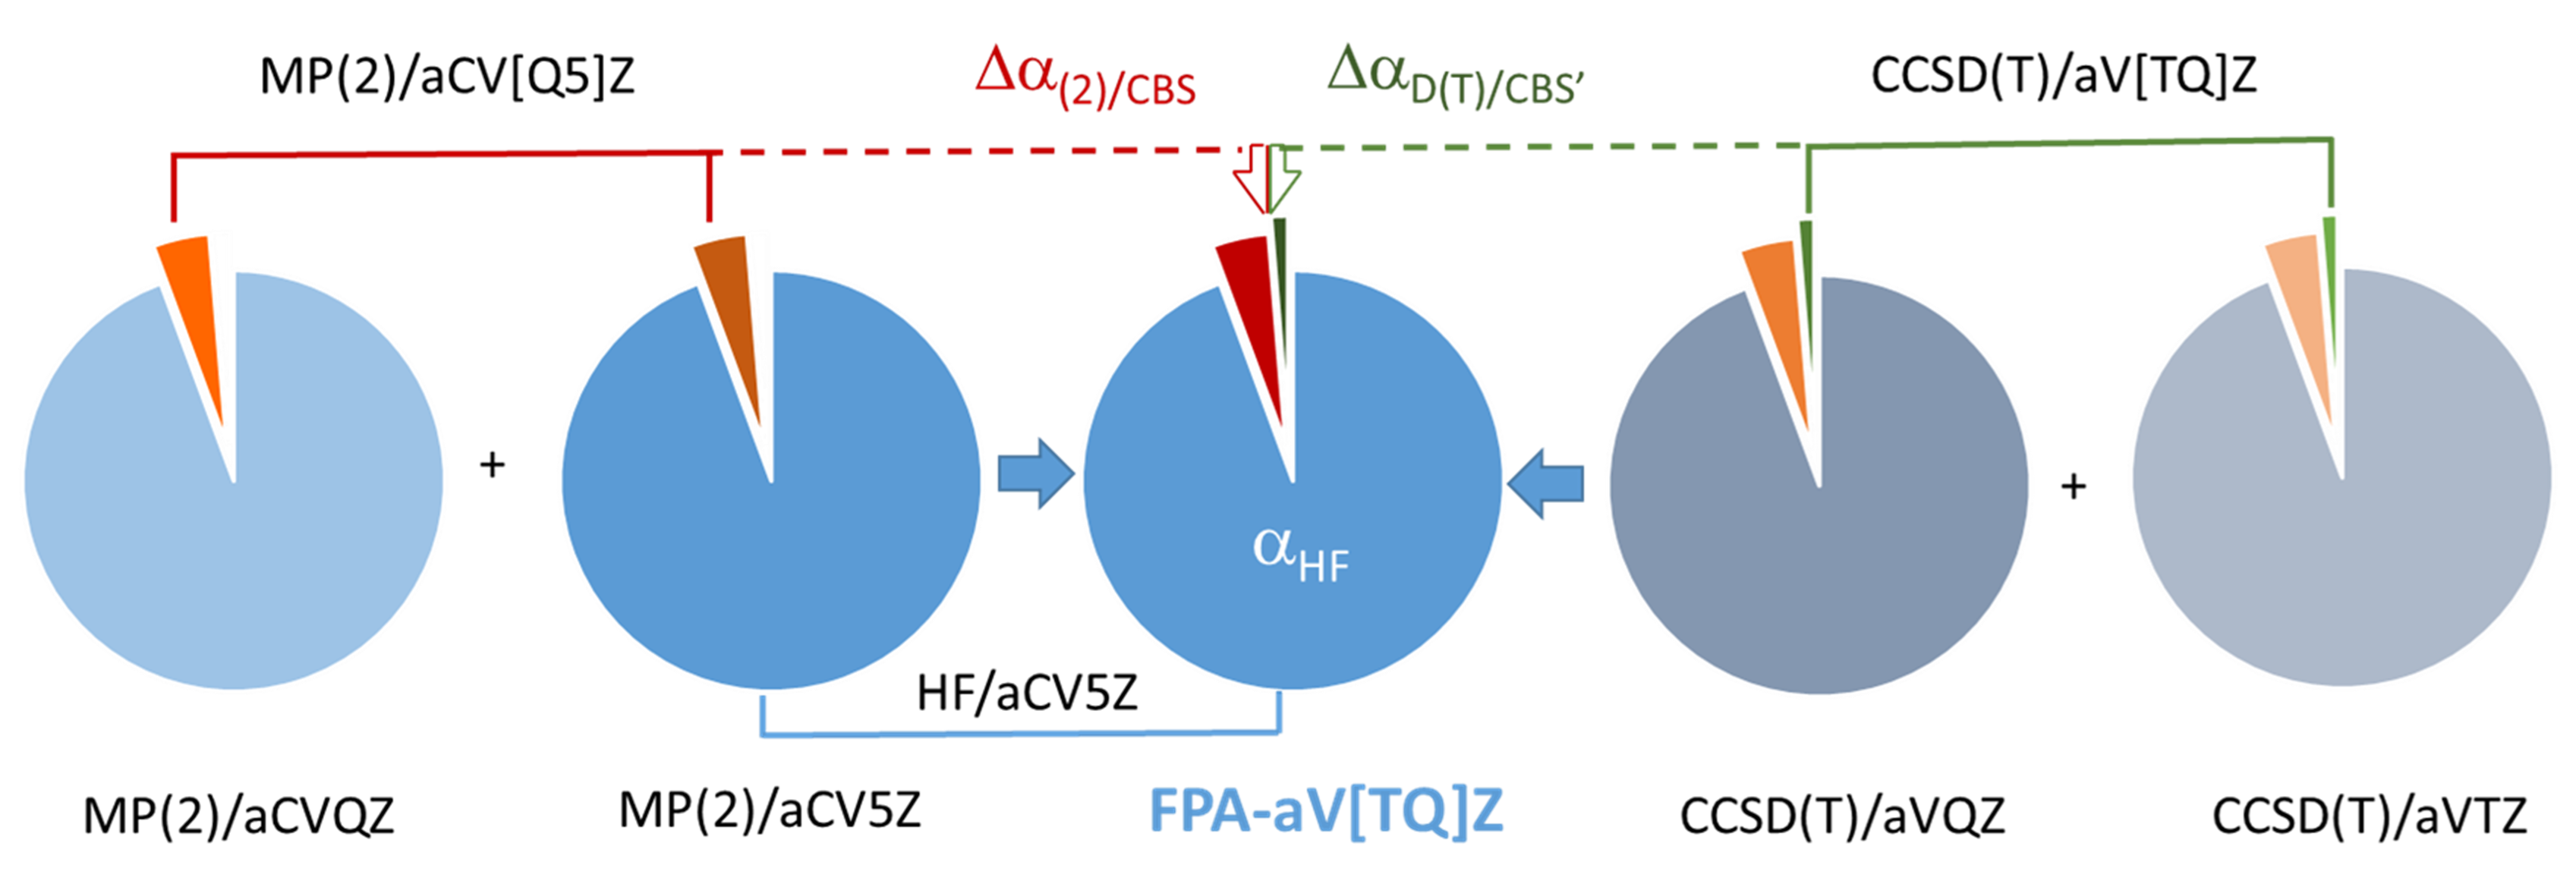
\includegraphics[width=0.9\textwidth]{assets/fig-1.png}
\end{figure}

以 FPA-aV[TQ]Z 作为例子,使用 FPA 策略的合理性通过图 \ref{fig.fig-1} 展示。HF 方法的结果占真实结果的绝对大头;但为正确描述物性,高质量的相关效应描述也是重要的。由于 HF 方法一般来说依基组基数 $\zeta$ 的收敛速度相当快\cite{Jensen-Jensen.TCA.2005, Karton-Martin.TCA.2006},因此许多 CBS 策略、包括 HH132 数据集的参考值,都对 HF 方法直接使用计算量上最大可承受的基组。而对于相关效应,则依基组基数 $\zeta$ 的增大,收敛速度相对缓慢。大多数情况下,MP2 占据相关效应的主要部分;因此,对 MP2 的大基组精确描述也非常重要。但对于更高阶的相关效应,一方面其绝对数值已然较小,另一方面数值对基组基数 $\zeta$ 的敏感性较小、或相对于 MP2 相关效应的收敛速度更快。对于后一方面所述的现象,目前已经在核磁屏蔽常数的计算\cite{Sun-Xu.JCP.2013, Wang-Xu.JCP.2018, Gregusova-Bartlett.JCTC.2010}、能量计算\cite{Truhlar-Truhlar.CPL.1998}等诸多情形下有所验证。因此,我们也会期望在极化率问题中,对于 CCSD(T) 相对于 MP2 之间的高级相关效应,使用较低等级基组或 CBS 外推方法,也可以提供一个合理的对高等级 CBS 外推方法的近似。本工作的其中一个重点,即是验证这个猜想的合理性。

\subsection{结论与讨论}

\subsubsection{RI 误差与数值差分误差}
\label{sec.5.3.1}

在本工作中,HF 与 MP2 的极化率是通过解析梯度给出,但引入了 RI 近似;CCSD 与 CCSD(T) 尽管未使用 RI 近似,但引入了数值差分误差。注意到表 \ref{tab.5.1} 中,将要汇报的 $\alpha_\textsf{CCSD(T)}$ 参考值是由 $\alpha^\text{anal}_\textsf{RI-MP2} + \Delta \alpha^\text{num}_\textsf{D(T)}$ 两部分构成;这两部分分别包含 RI 近似误差与数值差分误差。为了估计这部分误差的大小,我们考察了 HF 与 MP2 方法在 aVTZ 基组下、包含 RI 近似与不使用 RI 近似的同性极化率的结果。

我们看到,解析 RI-HF 与数值 HF 方法同性极化率之间相对方均根误差 $\text{RelRMSD} (\tilde \alpha_\textsf{RI-HF}^\text{anal}, \tilde \alpha^\text{num}_\textsf{HF})$,对于 HR46 与 T144 数据集,分别是 0.018\% 与 0.022\%。解析 RI-MP2 与数值 MP2 方法相关能贡献部分的方均根误差 $\text{RelRMSD} (\Delta \tilde \alpha^\text{anal}_\textsf{RI-(2)}, \Delta \tilde \alpha^\text{num}_\textsf{(2)}, \tilde \alpha^\text{num}_\textsf{MP2})$,对于两个数据集的误差均小于 0.01\%。这些误差都远远小于实验误差标准的 0.5\%,因此我们认为 RI 近似与数值差分误差对总的同性极化率 $\alpha_\textsf{CCSD(T)}$ 计算结果影响相当小,以至于可以忽略。我们猜测该结论对异性极化率 $\gamma_\textsf{CCSD(T)}$ 也同样适用。

我们还看到,对于相关贡献部分,自洽场收敛条件会对数值差分误差有一定影响。相关的数据与结论列于附录的 \ref{sec.5.s9} 小节。

\subsubsection{小体系的同性极化率基组收敛性}

在这两小节中,我们将对 14 个小体系 (\ce{Cl2}, \ce{CO}, \ce{CO2}, \ce{H2O}, \ce{N2}, \ce{NH3}, \ce{^3O2}, \ce{PH3}, \ce{SH2}, \ce{SiH4}, \ce{^3SO}, \ce{SO2}, \ce{FCN}, \ce{HCHS}) 作系统的基组收敛性分析,并基于此确定用于计算同性极化率的、高效的 FPA 模型。在该分析中,参考值由 CCSD(T)/CBS 计算所得:
\begin{equation*}
    \alpha_{\textsf{CCSD(T)}/\text{CBS}} = \alpha_{\textsf{HF}/\text{aCV5Z}} + \Delta \alpha_{\textsf{(2)}/\text{aCV[Q5]Z}} + \Delta \alpha_{\textsf{D(T)}/\text{aCV[Q5]Z}}
\end{equation*}
该参考值也对应了 HH132 数据集中最精确的 CBS 外推模型。详细的对 Dunning 系列基组的误差分析展示于表 \ref{tab.5.2}。

\begin{table}[ht]
    \centering
    \caption{14 个小体系同性极化率的相对方均根误差\tabnote{a}。}
    \label{tab.5.2}
    \begin{tabular}{cld{3.5}d{3.5}d{3.5}d{3.5}}
        \hline
          &              & \multicolumn{4}{c}{RelRMSD   error / \%}                \\ \cline{3-6}
    Level & \multicolumn{1}{c}{Basis set}    &
      \multicolumn{1}{c}{$\tilde \alpha_\textsf{HF}$\tabnote{b}}  &
      \multicolumn{1}{c}{$\Delta \tilde \alpha_\textsf{(2)}$\tabnote{c}}  &
      \multicolumn{1}{c}{$\Delta \tilde \alpha_\textsf{D}$\tabnote{c}} &
      \multicolumn{1}{c}{$\Delta \tilde \alpha_\textsf{D(T)}$\tabnote{c}}     \\ \hline
    2-$\zeta$ & aVDZ         & 3.385       & 0.853       & 1.113      & 0.787          \\
              & aCVDZ        & 3.376       & 0.799       & 1.053      & 0.748          \\ \hdashline
    3-$\zeta$ & aVTZ         & 0.703       & 0.516       & 0.406      & 0.297          \\
              & aCVTZ        & 0.671       & 0.385       & 0.339      & 0.270          \\
              & aV[DT]Z      &             & 0.535       & 0.155      & \textbf{0}.\textbf{144} \\
              & aCV[DT]Z     &             & 0.373       & 0.156\tabnote{d}     & 0.178\tabnote{d}         \\ \hdashline
    4-$\zeta$ & aVQZ         & 0.097       & 0.403       & 0.168      & 0.124          \\
              & aCVQZ        & 0.084       & 0.244       & 0.120      & 0.101          \\
              & aV[TQ]Z      &             & 0.359       & 0.111      & \textbf{0}.\textbf{086} \\
              & aCV[TQ]Z     &             & 0.179       & 0.131\tabnote{e}     & 0.096\tabnote{e}         \\ \hdashline
    5-$\zeta$ & aV5Z         & 0.024       & 0.233       & 0.082      & 0.065          \\
              & aCV5Z        & \multicolumn{1}{c}{\textbf{0}\tabnote{f}} & 0.125       & 0.061      & 0.052          \\
              & aV[Q5]Z      &             & 0.071       & 0.013      & \textbf{0}.\textbf{017} \\
              & aCV[Q5]Z     &             & \multicolumn{1}{c}{\textbf{0}\tabnote{f}} & \multicolumn{1}{c}{0\tabnote{f}}         & \multicolumn{1}{c}{0\tabnote{f}}             \\
    \hline
    \end{tabular}

    \raggedright
    \par\tabnote{a} 粗体的数字表示除参考值模型 FPA-aCV[Q5]Z 外,目前为止最佳的 FPA 模型;即依 3,4,5-$\zeta$ 分类下 FPA-aV[DT]Z、FPA-aV[TQ]Z 与 FPA-aV[Q5]Z。
    \par\tabnote{b} HF 同性极化率相对方均根误差为 $\text{RelRMSD} (\tilde \alpha_{\textsf{HF}/\text{basis}}, \tilde \alpha_{\textsf{HF}/\text{ref}}, \tilde \alpha_{\textsf{CCSD(T)}/\text{ref}})$。其中,$\tilde \alpha_{\textsf{HF}/\text{ref}}$ 指代的是 $\tilde \alpha_{\textsf{HF}/\text{aCV5Z}}$,$\tilde \alpha_{\textsf{CCSD(T)}/\text{ref}}$ 指代的时作为参考值的 $\alpha_{\textsf{CCSD(T)}/\text{CBS}}$。
    \par\tabnote{c} 相关能贡献的同性极化率相对方均根误差为 $\text{RelRMSD} (\Delta \tilde \alpha_{\textsf{corr}/\text{basis}}, \Delta \tilde \alpha_{\textsf{corr}/\text{ref}}, \tilde \alpha_{\textsf{CCSD(T)}/\text{ref}})$。其中,$\Delta \tilde \alpha_{\textsf{corr}}$ 可以是指 $\Delta \tilde \alpha_{\textsf{(2)}}$、$\Delta \tilde \alpha_{\textsf{D}}$ 或 $\Delta \tilde \alpha_{\textsf{D(T)}}$;而 $\Delta \tilde \alpha_{\textsf{corr}/\text{ref}}$ 指代的是 $\Delta \tilde \alpha_{\textsf{corr}/\text{aCV[Q5]Z}}$。
    \par\tabnote{d} 在排除 \ce{^3O2} 与 \ce{^3SO} 体系后,$\Delta \tilde \alpha_\textsf{D}$ 与 $\Delta \tilde \alpha_\textsf{D(T)}$ 的 RelRMSD 误差分别降至 0.126\% 与 0.136\%。对于这两个体系的基组收敛分析,将在附录 \ref{sec.5.s4} 小节展开。
    \par\tabnote{e} 在排除 \ce{Cl2} 体系后,$\Delta \tilde \alpha_\textsf{D}$ 与 $\Delta \tilde \alpha_\textsf{D(T)}$ 的 RelRMSD 误差分别降至 0.089\% 与 0.069\%。对于该体系的基组收敛分析,将在附录 \ref{sec.5.s4} 小节展开。
    \par\tabnote{f} 这些数值依据参考值的选取方式,从定义上是零。
\end{table}

首先,从具体的计算结果来看,首先可以肯定的是 HF 方法所给出的同性极化率确实占总同性极化率的主要部分;而 MP2 相关效应所贡献的部分,一般来说要比更高阶相关效应的部分要大一些。总的相关效应对于同性极化率上可能是正也可能是负;MP2 贡献部分与更高阶贡献部分的正负号经常是相反的。因此,为给出非常精确的极化率数据,我们需要仔细地分别考虑每个贡献部分的数值。

从表 \ref{tab.5.2} 总结的数据来看,我们发现对于 HF 方法而言,$\tilde \alpha_\textsf{HF}$ 的相对方均根误差在 2-$\zeta$ 基组下的误差相当大 ($> 3\%$)。因此,在极化率计算中,即使引入了弥散基组,2-$\zeta$ 级别下的计算结果也不具有实用性。在 3-$\zeta$ 基组下,$\tilde \alpha_\textsf{HF}$ 的相对方均根误差骤降至 0.7\%;到 4-$\zeta$ 基组时已经降至 0.1\% 以下,依基组基数 $\zeta$ 的收敛速度非常快。因此,对于 HF 方法,我们可以放心地认为在 aCV5Z 基组下,HF 方法的同性极化率已经非常精确、而不需要特意作额外 CBS 外推。该分析也印证了 HH132 数据集参考值构建过程中对 HF 方法的处理方式是合理的\cite{Hait-Head-Gordon.PCCP.2018}。

一个有意思的现象是,$\tilde \alpha_\textsf{HF}$ 的相对方均根误差在 2-$\zeta$ 与 3-$\zeta$ 等小基组下误差比对应的相关部分贡献 $\Delta \tilde \alpha_\textsf{corr}$ 更大;但当基组到 4-$\zeta$ 时,相关效应的误差比 HF 反过来更大。注意到 4-$\zeta$ 时,$\tilde \alpha_\textsf{HF}$ 的相对方均根误差是 0.1\% 以下;但对于 $\Delta \tilde \alpha_\textsf{(2)}$ 则在 aCVQZ 下是 0.244\%、aVQZ 下是 0.403\%。这些误差表现可以说明,MP2 相关效应贡献的部分依基组基数 $\zeta$ 的收敛速度相对于 HF 而言慢得多;这也与 HH132 的测评结论一致\cite{Hait-Head-Gordon.PCCP.2018}。同时,我们看到,若在 4-$\zeta$ 与 5-$\zeta$ 级别的基组上引入 CBS 外推,则误差可以降低大约 0.05\%;并且当引入核层基函数时,极化率的误差表现普遍更低一些。考虑到即使是 4-$\zeta$ 的 CBS 下 $\Delta \tilde \alpha_\textsf{(2)}$ 仍有一定的误差、且在引入了 RI 近似后 MP2 的计算量在更大的 5-$\zeta$ 下是可接受的,那么为了与 HH132 的参考值维持尽可能相似的精度,我们采用 aCV[Q5]Z 的 CBS 外推模型计算 $\Delta \alpha_\textsf{(2)}$ 的参考值。至此,剩下来的提升同性极化率的精度空间,就是如何精确且高效地计算 $\Delta \alpha_\textsf{D(T)}$ 的结果。

幸运的是,从表 \ref{tab.5.2} 的数据来看,$\Delta \tilde \alpha_\textsf{D(T)}$ 的相对方均根误差,比起 $\Delta \tilde \alpha_\textsf{(2)}$ 来说依基组基数 $\zeta$ 的收敛速度更快且误差更小。举例而言,对于 aVTZ 与 aVQZ 基组,$\Delta \tilde \alpha_\textsf{D(T)}$ 相对方均根误差为 0.297\% 与 0.124\%,在数值上与收敛速度上都明显快于 $\Delta \tilde \alpha_\textsf{(2)}$ 的 0.516\% 与 0.403\%。对于 aVTZ 与 aVQZ 基组,引入 CBS 外推得到 aV[DT]Z 与 aV[TQ]Z 后,其误差可以有大约一半的降幅,且两个 CBS 外推模型的误差都小于 0.2\%。同时,aV[Q5]Z 外推模型相比于 aCV[Q5]Z 的误差是非常小的 0.017\%。

需要指出,对于如 $\Delta \alpha_\textsf{D(T)}$ 高阶的相关贡献部分,基组中引入核层的函数不仅会大幅增加计算消耗,同时对部分体系也会破坏收敛趋势、以至于 CBS 外推模型失效。举例而言,对于我们目前研究的 14 个小体系,$\Delta \tilde \alpha_\textsf{D(T)}$ 在 aCV[DT]Z 外推下的相对方均根误差是 0.178\%,比 aV[DT]Z 的 0.144\% 要更大;只有当排除了 \ce{^3O2} 与 \ce{^3SO} 这两个异常体系,误差才能降至比 aV[DT]Z 更低的 0.136\%。类似的情形在 aCV[TQ]Z 与 aV[TQ]Z 的比较中也存在。对于这些异常体系的讨论,我们在附录 \ref{sec.5.s4} 小节中展开。

综上所述,我们建议对同性极化率使用的 FPA 模型是
\begin{equation}
    \alpha_{\text{FPA-aV[}XY\text{]Z}} = \alpha_{\textsf{HF}/\text{aCV5Z}} + \Delta \alpha_{\textsf{(2)}/\text{aCV[Q5]Z}} + \Delta \alpha_{\textsf{D(T)}/\text{aV[}XY\text{]Z}}
\end{equation}
其中,$[XY] \in \mathrm{[DT], [TQ], [Q5]}$,具体的取值依据分子大小而定。相对于最佳的理论计算模型 $\alpha_{\text{FPA-aCV[Q5]Z}}$,$\alpha_{\text{FPA-aV[}XY\text{]Z}}$ 的误差来源仅出现在 $\Delta \tilde \alpha_\textsf{D(T)}$ 的基组不完备程度。因此,从表 \ref{tab.5.2} 的数据来看,FPA-aV[DT]Z、FPA-aV[TQ]Z、FPA-aV[Q5]Z 在计算同性极化率时的相对方均根误差分别是 0.144\%、0.086\%、0.017\%。这些 FPA 模型的误差都明显小于我们的目标精度 0.5\%。我们期待这些 FPA 模型应用于更大体系、如 HR46 或 T144 中更大的分子时,计算精度可以与 HH132 的参考值相比较。

\subsubsection{自旋非极化小体系的异性极化率基组收敛性}

本工作同样考虑了异性极化率 $\gamma$ 的计算问题。在这一小节中,我们考虑 7 个自旋非极化分子 (\ce{Cl2}, \ce{CO}, \ce{CO2}, \ce{FCN}, \ce{HCHS}, \ce{N2}, \ce{SO2}) 的基组收敛性与 CBS 外推精度,以确定对异性极化率计算所适合使用的 FPA 模型。相对于同性极化率分析过程中使用的 14 个体系,我们排除了 5 个自旋非极化与 2 个自旋极化分子。其中,5 个自旋非极化分子 (\ce{H2O}, \ce{H2S}, \ce{NH3}, \ce{PH3}, \ce{SiH4}) 由于异性极化率的数值过小 (小于 0.5 $\text{\AA}^3$),使用相对方均根误差不是非常合理。在附录的\alert{表 S7}中,我们使用绝对值的方均根误差作为判标,将这 5 个小分子引入基组收敛性与 CBS 外推精度分析,并且认为引入这 5 个异性极化率 $\gamma$ 较小的体系不影响结论。同时,由于 HR46 与 T144 的绝大多数分子都是自旋非极化分子;在对异性极化率的讨论中,我们的讨论将局限于自旋非极化体系,因此排除了自旋计划体系 \ce{^3O2} 与 \ce{^3SO}。详细的对 Dunning 系列基组的误差分析展示于表 \ref{tab.5.3}。

\begin{table}[ht]
    \centering
    \caption{7 个自旋非极化小体系异性极化率的相对方均根误差\tabnote{a}。}
    \label{tab.5.3}
    \begin{tabular}{cld{3.5}d{3.5}d{3.5}d{3.5}}
        \hline
          &              & \multicolumn{4}{c}{RelRMSD   error / \%}                \\ \cline{3-6}
    Level & \multicolumn{1}{c}{Basis set}    &
      \multicolumn{1}{c}{$\tilde \gamma_\textsf{HF}$\tabnote{b}}  &
      \multicolumn{1}{c}{$\Delta \tilde \gamma_\textsf{(2)}$\tabnote{b}}  &
      \multicolumn{1}{c}{$\Delta \tilde \gamma_\textsf{D}$\tabnote{b}} &
      \multicolumn{1}{c}{$\Delta \tilde \gamma_\textsf{D(T)}$\tabnote{b}}     \\ \hline
    2-$\zeta$   & aVDZ         & 5.825       & 1.161       & 1.515      & 0.864           \\
          & aCVDZ        & 5.939       & 1.137       & 1.320      & 0.842           \\ \hdashline
    3-$\zeta$   & aVTZ         & 1.632       & 0.468       & 0.536      & 0.328           \\
          & aCVTZ        & 1.127       & 0.420       & 0.395      & 0.313           \\
          & aV[DT]Z  &             & 0.603       & 0.200      & \textbf{0}.\textbf{177}  \\
          & aCV[DT]Z &             & 0.408       & 0.173      & 0.177           \\ \hdashline
    4-$\zeta$   & aVQZ         & 0.508       & 0.390       & 0.276      & 0.186           \\
          & aCVQZ        & 0.203       & 0.251       & 0.122      & 0.101           \\
          & aV[TQ]Z  &             & 0.417       & 0.246c     & \textbf{0}.\textbf{230}\tabnote{c} \\
          & aCV[TQ]Z &             & 0.229       & 0.168      & 0.131           \\ \hdashline
    5-$\zeta$   & aV5Z         & 0.130       & 0.173       & 0.129      & 0.091           \\
          & aCV5Z        & \multicolumn{1}{c}{\textbf{0}\tabnote{d}} & 0.129       & 0.063      & 0.052           \\
          & aV[Q5]Z  &             & 0.115       & 0.070      & \textbf{0}.\textbf{037}  \\
          & aCV[Q5]Z     &             & \multicolumn{1}{c}{\textbf{0}\tabnote{d}} & \multicolumn{1}{c}{0\tabnote{d}}         & \multicolumn{1}{c}{0\tabnote{d}}             \\
    \hline       
    \end{tabular}

    \raggedright
    \par\tabnote{a} 粗体的数字表示除参考值模型 FPA-aCV[Q5]Z 外,目前为止最佳的 FPA 模型;即依 3,4,5-$\zeta$ 分类下 FPA-aV[DT]Z、FPA-aV[TQ]Z 与 FPA-aV[Q5]Z。
    \par\tabnote{b} 这些记号的定义参考表 \ref{tab.5.2};所有同性极化率 $\alpha$ 的记号替换为异性极化率 $\gamma$ 记号。
    \par\tabnote{c} 在排除 \ce{Cl2} 与 \ce{HCHS} 体系后,$\Delta \tilde \gamma_\textsf{D}$ 与 $\Delta \tilde \gamma_\textsf{D(T)}$ 的 RelRMSD 误差分别降至 0.195\% 与 0.134\%。对于该体系的基组收敛分析,将在附录 \ref{sec.5.s5} 小节展开。
    \par\tabnote{d} 这些数值依据参考值的选取方式,从定义上是零。
\end{table}

异性极化率 $\gamma$ 在基组收敛性上的表现,与同性极化率 $\alpha$ 在不少特征上是相似的;譬如高阶的相关效应贡献普遍小于 MP2 相关效应的贡献、且远小于 HF 贡献;HF 方法的收敛速度快于 MP2 与更高阶相关效应的收敛速度等等。但与同性极化率 $\alpha$ 不同地,$\tilde \gamma_\textsf{HF}$ 在较大的 4-$\zeta$ 基组下也仍然有很大的误差:aVQZ 的误差 0.508\% 已经超过了我们的目标精度 0.5\%;因此,不能简单地认为 5-$\zeta$ 已经非常接近基组收敛极限。但如果从 $\tilde \gamma_\textsf{HF}$ 较快的收敛速度来看,我们预期 aCV5Z 到基组极限的误差大约在 0.1\% 左右。

对于 MP2 相关贡献部分 $\Delta \tilde \gamma_\textsf{(2)}$,我们发现若基组中没有核函数的描述,那么以 aV[DT]Z 与 aV[TQ]Z 为例的 CBS 外推,其误差反而要比 aVTZ 与 aVQZ 更大。这表明精确地计算异性极化率 $\gamma$ 的计算相比于同性极化率 $\alpha$,确实更有挑战性。但若基组中引入核函数,一方面 CBS 外推模型 aCV$[XY]$Z ($Y > X$) 的误差确实相比于 aCV$Y$Z 的误差有所减小;另一方面,这些 CBS 外推模型下的 $\Delta \tilde \gamma_\textsf{(2)}$ 相对方均根误差与表 \ref{tab.5.2} 所示的 $\Delta \tilde \alpha_\textsf{(2)}$ 处在同样的误差水平上。因此,我们认为 $\Delta \tilde \gamma_{\textsf{(2)}/\text{aCV[Q5]Z}}$ 相比于基组极限之间的精度,与 $\Delta \tilde \alpha_{\textsf{(2)}/\text{aCV[Q5]Z}}$ 是相当的。

对于 MP2 之上的更高阶相关效应,仍然非常幸运的是,$\Delta \tilde \gamma_\textsf{D(T)}$ 不仅是在误差数值上更小、也在依基组基数 $\zeta$ 收敛速度上比 $\Delta \tilde \gamma_\textsf{(2)}$ 更快。大多数情形下,对于我们考察的 7 个自旋非极化小体系,更大的基组下 $\Delta \tilde \gamma_\textsf{D(T)}$ 的计算结果更精确,CBS 外推模型一般来说也可以有效降低误差。尽管我们看到对于 aV[TQ]Z 的 CBS 外推模型下,\ce{Cl2} 与 \ce{HCHS} 的收敛趋势较为特殊,我们也将在附录 \ref{sec.5.s5} 中作更细致的讨论;但即使包含了这两个特例情形,不同级别的 CBS 外推模型给出的 $\Delta \tilde \gamma_\textsf{D(T)}$ 误差都小于 0.3\%。对比 aV[$XY$]Z 与 aCV[$XY$]Z 这两类 CBS 外推模型,我们认为计算消耗更大的、引入核函数的 aCV[$XY$]Z 在误差表现上,没有明显好于 aV[$XY$]Z。因此,我们认为不引入核函数,给出的 $\Delta \tilde \gamma_\textsf{D(T)}$ 结果也是可接受的。类似的讨论也适用于 $\Delta \tilde \gamma_\textsf{D}$。

综上所述,我们建议对自旋非极化的异性极化率使用的 FPA 模型,与同性极化率的情形相同:
\begin{equation}
    \gamma_{\text{FPA-aV[}XY\text{]Z}} = \gamma_{\textsf{HF}/\text{aCV5Z}} + \Delta \alpha_{\textsf{(2)}/\text{aCV[Q5]Z}} + \Delta \gamma_{\textsf{D(T)}/\text{aV[}XY\text{]Z}}
\end{equation}
从表 \ref{tab.5.3} 与上述讨论中,我们认为对于各种 FPA-aV[$XY$]Z 模型,其误差相比于作为最精确结果的 FPA-aCV[Q5]Z,应会小于 0.3\%。我们也期待这些 FPA 模型可以应用到更大体系的计算,并且由于基组不完备而引起的误差不会超过实验误差精度 0.5\%。

最后,我们指出,我们所测评的自旋极化体系 (\ce{^3O2}, \ce{^3SO}) 的异性极化率,其收敛趋势与精度都相当有挑战性。这些测评在附录 \ref{sec.5.s5} 中展示。因此,若要对各类体系的异性极化率 $\gamma$ 作更全面的研究,那么需要在表 \ref{tab.5.3} 的基础上引入更多的自旋非极化体系。

\subsubsection{极化率参考值的更新}

我们现在将 FPA-aV[DT]Z、FPA-aV[TQ]Z、FPA-aV[Q5]Z 这三个 FPA 模型,应用于 HR46 与 T144 数据集的同性极化率 $\alpha$ 与异性极化率 $\gamma$ 参考值的计算,以将提升参考值的精度更新到 CCSD(T)/CBS 的级别上。出于计算资源限制、但同时要以尽可能高的精度给出数据,我们需要对 HR46 与 T144 分出子集;不同的子集将使用不同级别的 FPA 模型。表 \ref{tab.5.4} 展示了数据集分割的总体情况。需要指出,该数据分割方式并非毫无偏向性:以 HR46 数据集为例,其 Set I 子集仅包含无机分子、而 Set III 的大多数分子都具有芳环。详细的数据集分割情况参考\alert{附录具体数据}。

\begin{table}[ht]
    \centering
    \caption{数据集依 CCSD(T) 计算能力限制的分割总体情况、以及分割后子集在计算极化率时对应使用的 FPA 模型。}
    \label{tab.5.4}
    \begin{tabular}{ccccc}
    \hline
    Dataset & Subset  & Number of species & Number of atoms & Reference FPA Scheme \\ \hline
    HR46    & Set I   & 14                & 2--5            & FPA-aV[Q5]Z      \\
            & Set II  & 14                & 5--11           & FPA-aV[TQ]Z      \\
            & Set III & 18                & 9--15           & FPA-aV[DT]Z      \\
    T144    & Set I   & 34                & 3--8            & FPA-aV[TQ]Z      \\
            & Set II  & 110               & 8--14           & FPA-aV[DT]Z      \\ \hline
    \end{tabular}
\end{table}

对于 HR46 Set I,其最适用的 FPA 模型是 FPA-aV[Q5]Z,它也是本工作中所有 FPA 模型近似中最精确的。对于该子集,FPA-aV[TQ]Z 与 FPA-aV[DT]Z 由于计算量小,数据因此较为容易获得。同样地,HR46 Set II 与 T144 Set I 最适用的 FPA 模型是 FPA-aV[TQ]Z;它们也有更低一等级的 FPA-aV[DT]Z 模型。对于这些分子体系较小、可以应用更昂贵的 FPA 模型的子集,我们测评了这些子集下不同 FPA 模型之间的相对误差;数据展现在表 \ref{tab.5.5} 与 \ref{tab.5.6} 中。可以看到,所有纳入误差分析的数据子集中,同性极化率的误差均小于 0.2\%、异性极化率的误差均小于 0.3\%,即所有情形下的误差都大幅小于目标精度 0.5\%。这也意味着,尽管 FPA-aV[DT]Z 与 FPA-aV[TQ]Z 的计算代价较低,但精度上没有比最精确地 FPA-aV[Q5]Z 低太多;这三种 FPA 模型的精度都是令人满意的。

\begin{table}[ht]
    \centering
    \caption{HR46 与 T144 子集下同性极化率 $\Delta \tilde \alpha_\textsf{CCSD(T)}$ 在不同 FPA 模型下的相对方均根误差\tabnote{a}。}
    \label{tab.5.5}
    \begin{tabular}{ccccc}
    \hline
    Dataset & Subset & Scheme & Reference & RelRMSD / \% \\ \hline
    HR46    & I      & FPA-aV[DT]Z & FPA-aV[Q5]Z & 0.158 \\
            & I      & FPA-aV[TQ]Z & FPA-aV[Q5]Z & 0.127 \\
            & II     & FPA-aV[DT]Z & FPA-aV[TQ]Z & 0.091 \\
    T144    & I      & FPA-aV[DT]Z & FPA-aV[TQ]Z & 0.127 \\ \hline
    \end{tabular}

    \raggedright
    \par\tabnote{a} 相对误差以 $\text{RelRMSD} (\tilde \alpha_{\textsf{CCSD(T)}/\text{Scheme}}, \tilde \alpha_{\textsf{CCSD(T)}/\text{Reference}})$ 呈现。
\end{table}

\begin{table}[ht]
    \centering
    \caption{HR46 与 T144 子集下异性极化率 $\Delta \tilde \gamma_\textsf{CCSD(T)}$ 在不同 FPA 模型下的相对方均根误差\tabnote{a}。}
    \label{tab.5.6}
    \begin{tabular}{ccccc}
    \hline
    Dataset & Subset & Scheme & Reference & RelRMSD / \% \\ \hline
    HR46    &  I\tabnote{b} & FPA-aV[DT]Z & FPA-aV[Q5]Z & 0.197 \\
            &  I\tabnote{b} & FPA-aV[TQ]Z & FPA-aV[Q5]Z & 0.277 \\
            & II\tabnote{c} & FPA-aV[DT]Z & FPA-aV[TQ]Z & 0.225 \\
    T144    &  I\tabnote{d} & FPA-aV[DT]Z & FPA-aV[TQ]Z & 0.205 \\ \hline
    \end{tabular}

    \raggedright
    \par\tabnote{a} 相对误差以 $\text{RelRMSD} (\tilde \gamma_{\textsf{CCSD(T)}/\text{Scheme}}, \tilde \gamma_{\textsf{CCSD(T)}/\text{Reference}})$ 呈现。统计误差时,仅考虑 $\gamma_{\textsf{CCSD(T)}}$ 大于 0.5 $\text{\AA}{}^{3}$ 的体系。
    \par\tabnote{b} HR46 Set I 的 14 个分子中,6 个被纳入误差统计。
    \par\tabnote{c} HR46 Set II 的 14 个分子中,12 个被纳入误差统计。
    \par\tabnote{d} T144 Set I 的 34 个分子中,32 个被纳入误差统计。
\end{table}

尽管我们对 FPA-aV[$XY$]Z 模型应用于异性极化率 $\gamma$ 在自旋非极化体系 (如 \ce{^3O2}, \ce{^3SO}, \ce{^2NO}) 下的计算,是否其精度达到目标需求,这个问题上我们报以保留的态度;但在我们关心的 HR46 与 T144 数据集中,仅有 3 个分子是自旋极化、且它们足够小以至于可以通过最高精度的 FPA-aV[Q5]Z 计算。而 HR46 与 T144 数据集剩下的所有分子均为自旋非极化的;对于这些体系可以应用 FPA 模型作高精度计算。因此,对于提升数据集精度的目的而言,表 \ref{tab.5.4} 的策略是完全有效的。通过 FPA-aV[$XY$]Z 模型提升精度后的、具体的 HR46 与 T144 极化率数据列于\alert{附录具体数据}。

\subsubsection{对 HF、MP2 与 CCSD 的极化率测评}

如前所述,参考值的极化率计算中,HF 方法通过 aCV5Z 给出、MP2 相关部分通过 aCV[Q5]Z 给出。对于 CCSD 方法,我们使用了与 CCSD(T) 相同的 FPA 模型给出结果,具体的情形总结在表 \ref{tab.5.4} 中。

\newpage

\subsection{附录}

\subsubsection{HR46 与 T144 数据集分子结构}

\begin{figure}[H]
    \centering
    \caption{HR46 数据集分子结构。}
    \label{fig.fig-s1}
    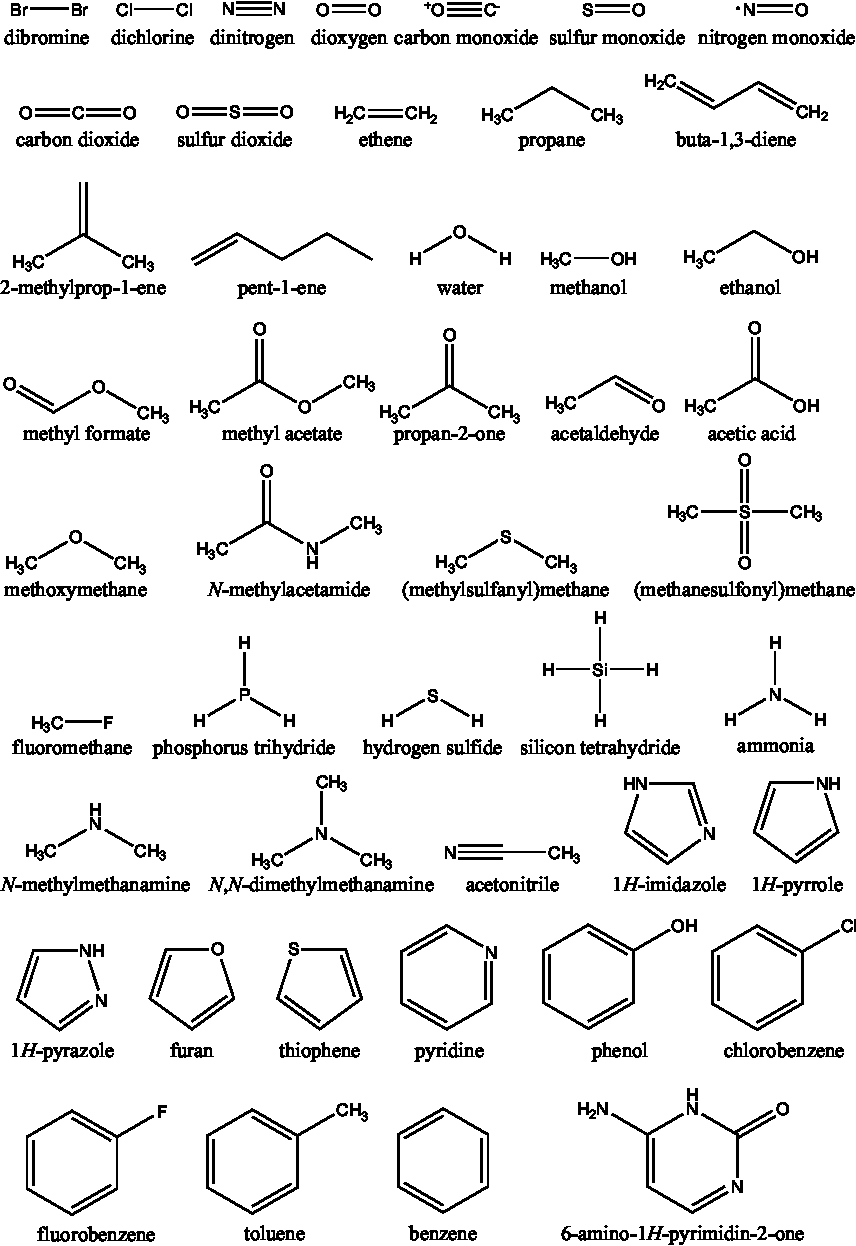
\includegraphics[width=0.85\textwidth]{assets/fig-s1.pdf}
\end{figure}

\begin{figure}[H]
    \centering
    \caption{T144 数据集分子结构。}
    \label{fig.fig-s2-1}
    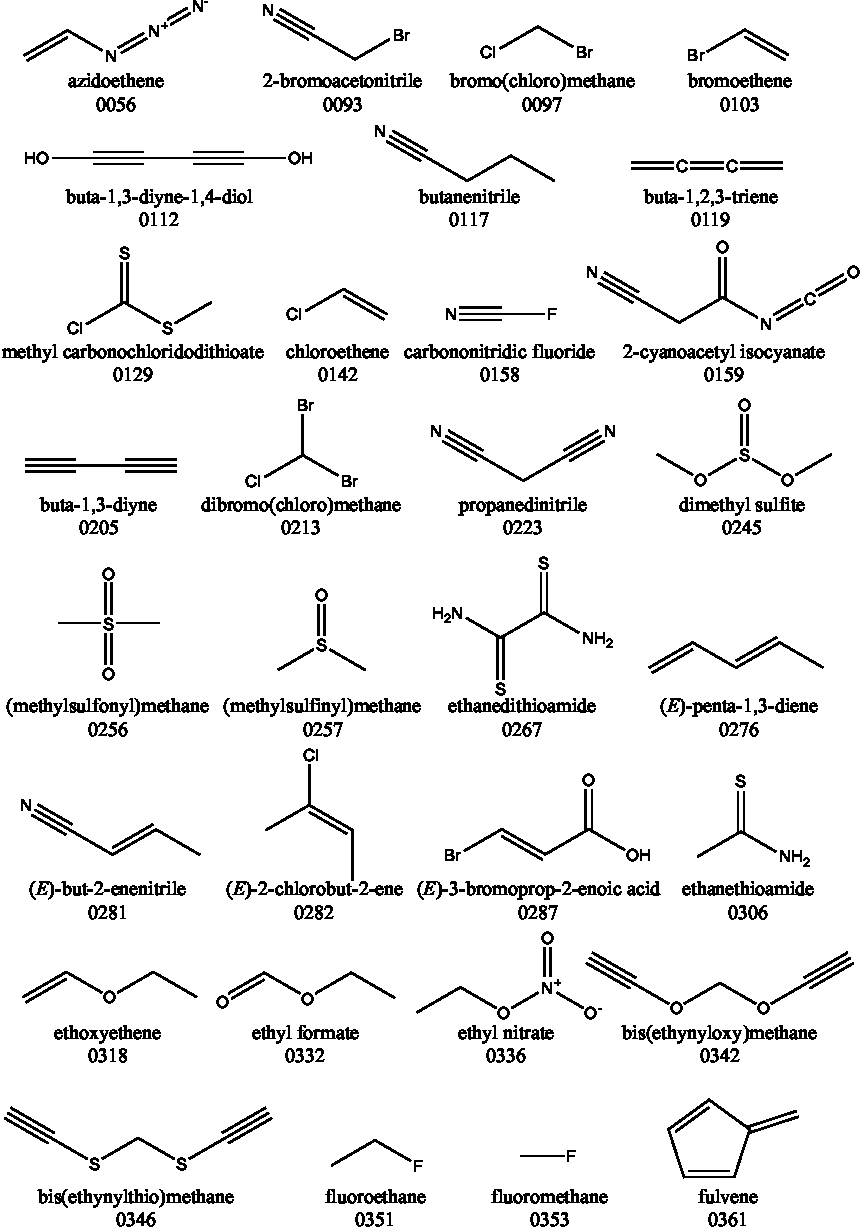
\includegraphics[width=0.85\textwidth]{assets/fig-s2-1.pdf}
\end{figure}

\setcounter{figure}{\value{figure} - 1}

\begin{figure}[H]
    \centering
    \caption{(续图)}
    \label{fig.fig-s2-2}
    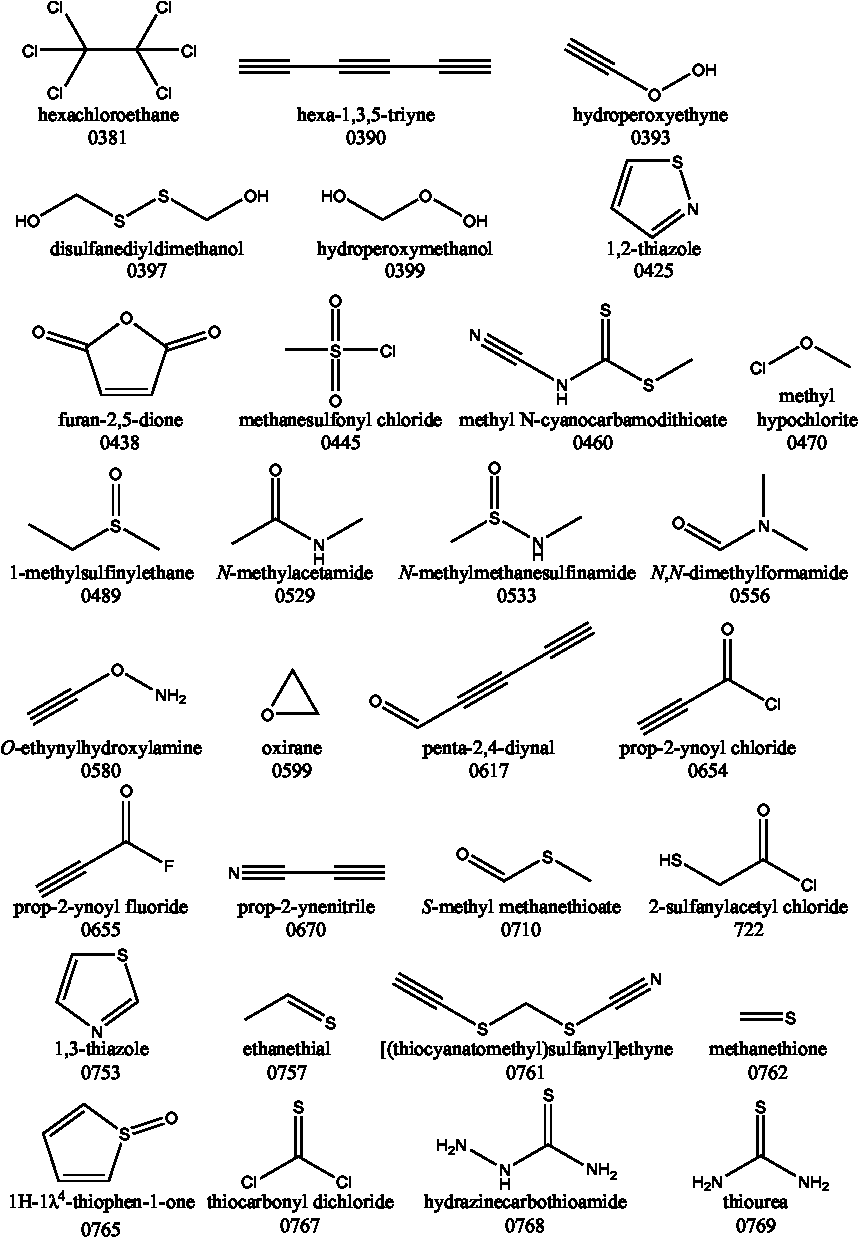
\includegraphics[width=0.85\textwidth]{assets/fig-s2-2.pdf}
\end{figure}

\setcounter{figure}{\value{figure} - 1}

\begin{figure}[H]
    \centering
    \caption{(续图)}
    \label{fig.fig-s2-3}
    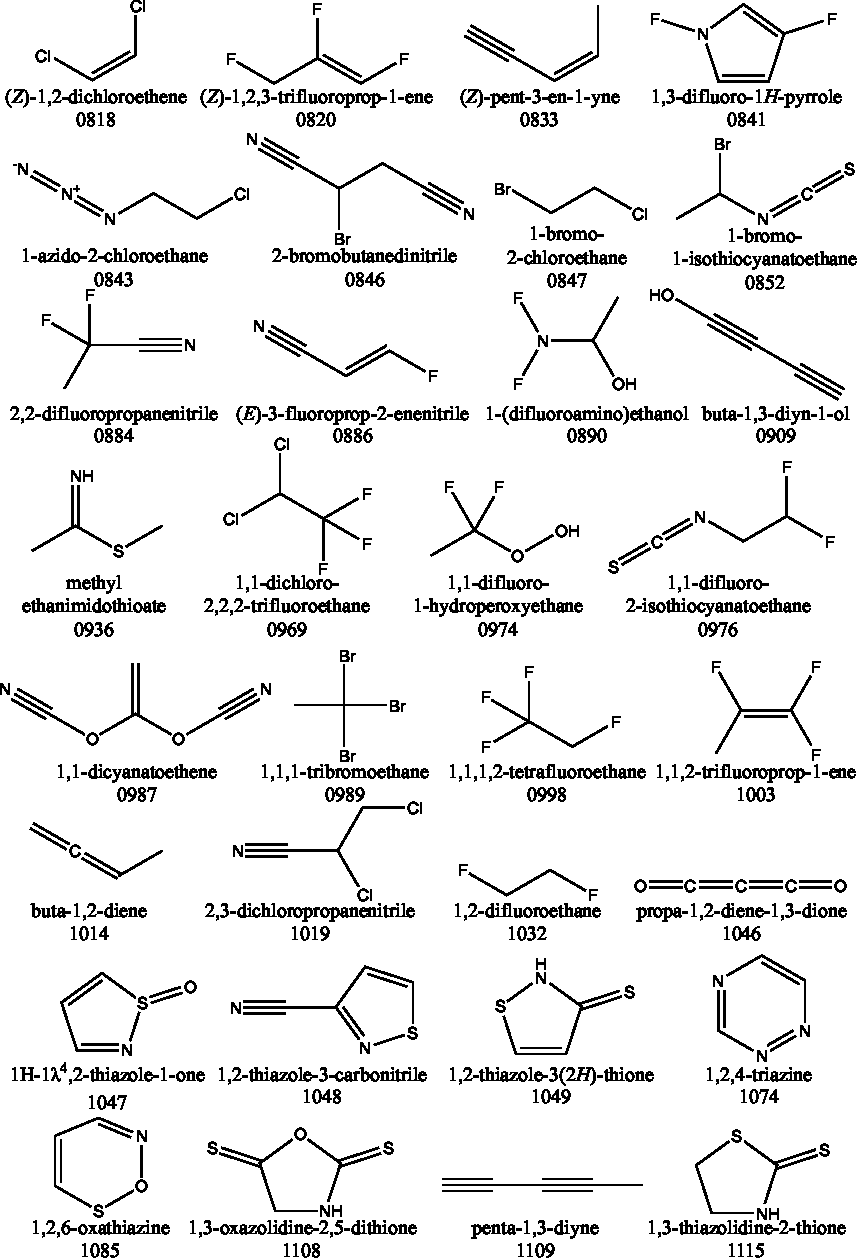
\includegraphics[width=0.85\textwidth]{assets/fig-s2-3.pdf}
\end{figure}

\setcounter{figure}{\value{figure} - 1}

\begin{figure}[H]
    \centering
    \caption{(续图)}
    \label{fig.fig-s2-4}
    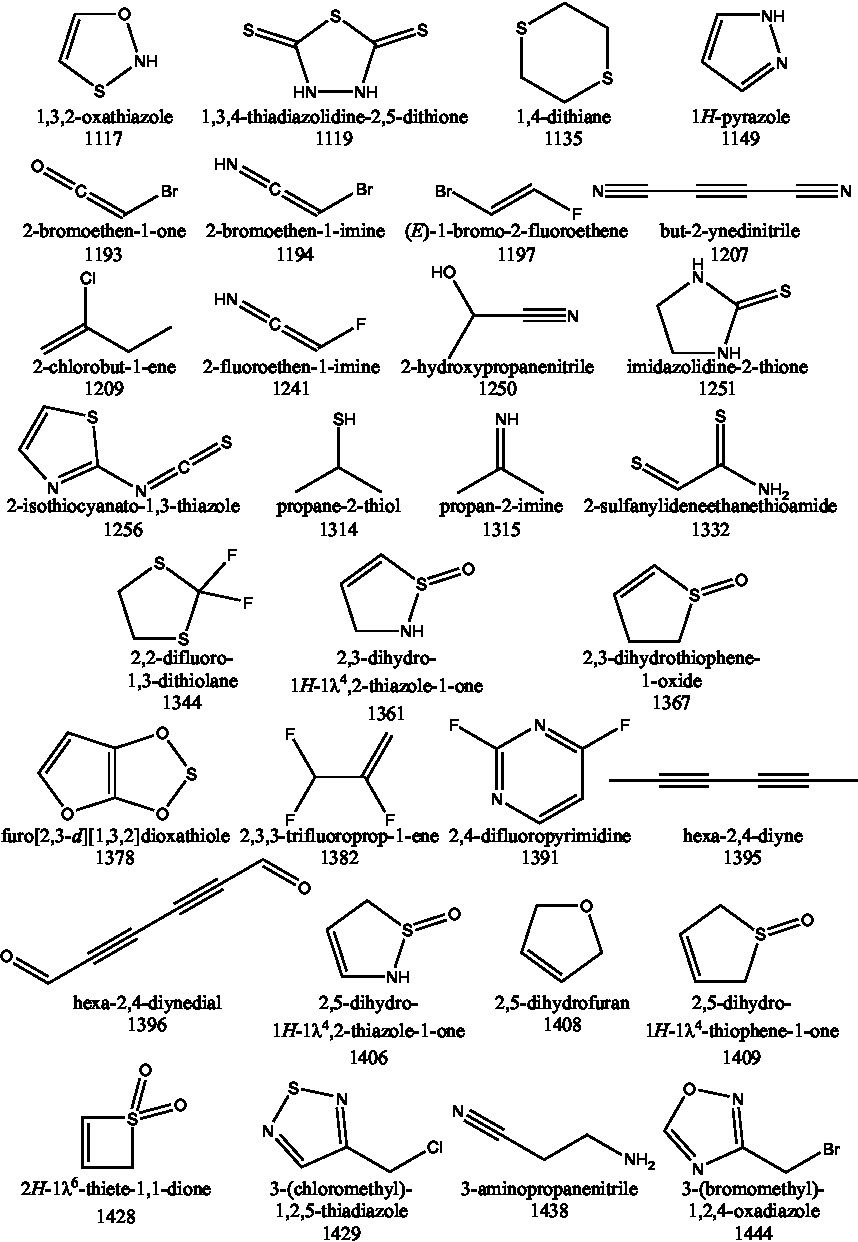
\includegraphics[width=0.85\textwidth]{assets/fig-s2-4.pdf}
\end{figure}

\setcounter{figure}{\value{figure} - 1}

\begin{figure}[H]
    \centering
    \caption{(续图)}
    \label{fig.fig-s2-5}
    \includegraphics[width=0.85\textwidth]{assets/fig-s2-5.pdf}
\end{figure}

\newpage

\subsubsection{体系名称的更改}
\label{sec.T145-HR46-name-change}

本工作会对原先 T144 与 HR46 数据集的化合物名称作一定更改。我们尽量依照 IUPAC 推荐命名规则 (PIN, \underline{P}referred \underline{I}UPAC \underline{N}ame) 进行命名\cite{Favre-Powell.RSC.2013}。举例而言,“acetone”(丙酮) 将被命名为“propane-2-one”(丙-2-酮)。这类名称更改是平凡的。

HR46 原文献\cite{Hickey-Rowley.JPCA.2014}中,正文中名称为“thymine”的分子应命名为“cytosine”(胞嘧啶,或 PIN 命名 6-amino-1\textit{H}-pyrimidin-2-one)。其补充信息中的命名是正确的。

T144 数据集中,我们依据 TABS 数据库所提供的分子坐标文件,对下述 4 个分子的名称作勘定,并示于表 \ref{tab.T144-name-errata}。

\begin{table}[H]
    \centering
    \caption{T144 数据集名称勘定。}
    \label{tab.T144-name-errata}
    \begin{tabular}{lll}
    \hline
    ID   & Original   Name                & Updated   Name                    \\ \hline
    0129 & carbonochloridodithioic   acid & methyl   carbonochloridodithioate \\
    0399 & hydroxymethylperoxide          & hydroperoxymethanol               \\
    1193 & 2-bromoethanone                & 2-bromoethen-1-one                \\
    1630 & 5-methyl-2\textit{H}-tetrazole          & 5-methyl-1\textit{H}-tetrazole             \\ \hline
    \end{tabular}
\end{table}

\subsubsection{对有限差分误差的分析}
\label{sec.5.s9}

对同性极化率 $\alpha$ 所作的因有限差分而导致误差的分析列于表 \ref{tab.5.s8}。作为参照的数值是解析梯度所计算得到的极化率。我们假定对异性极化率 $\gamma$ 应有类似的结论。在该分析中,我们将使用两种自洽场收敛判据。需要指出,解析梯度极化率的精度也受机器精度、自洽场收敛精度与 CP-HF 方程收敛精度等要素影响;但在这段分析中,我们假定这些影响要素可以忽略不计。

\begin{table}[ht]
    \centering
    \caption{HR45 数据集同性极化率因数值导数而起的相对方均差 (RelRMSD)\tabnote{a}。}
    \label{tab.5.s8}
    \begin{tabular}{ccccccc}
    \hline
    & \multicolumn{2}{c}{$\alpha_\textsf{MP2}$ / \%\tabnote{b}} & \multicolumn{2}{l}{$\alpha_\textsf{HF}$ / \%\tabnote{c}} & \multicolumn{2}{l}{$\Delta \alpha_\textsf{(2)}$ / \%\tabnote{d}} \\
    Interval $h$ / au & loose\tabnote{e}         & tight\tabnote{f}        & loose\tabnote{e}        & tight\tabnote{f}        & loose\tabnote{e}         & tight\tabnote{f}         \\
    \hline
    0.0005            & 1.625          & 0.000         & 0.000         & 0.000         & 1.625          & 0.000          \\
    0.0010            & 0.395          & 0.002         & 0.001         & 0.001         & 0.395          & 0.001          \\
    0.0020            & 0.046          & 0.006         & 0.005         & 0.005         & 0.046          & 0.002          \\
    0.0040            & 0.031          & 0.025         & 0.019         & 0.019         & 0.020          & 0.008          \\
    0.0080            & 0.101          & 0.101         & 0.075         & 0.075         & 0.033          & 0.033          \\
    0.0160            & 0.415          & 0.415         & 0.309         & 0.309         & 0.138          & 0.138          \\
    \hline
    \end{tabular}

    \raggedright
    \par\tabnote{a} 该表格数据是通过 \textsc{PySCF} 结合扩展程序 \textsc{dh},以 aVTZ 级别基组计算,对 HR45 数据集 (除去了 \ce{^2NO} 分子的 HR46 数据集),在不同的自洽场收敛条件、以及不同的有限差分外场强度 $h$ 下所给出 (其意义在式 (\ref{eq.pol-findiff-alpha-def}, \ref{eq.pol-findiff-gamma-def}) 给出)。所有计算都使用 RI 近似,且 RI 辅助基选用 \textsc{PySCF} 默认的 ETB 给出。
    \par\tabnote{b} $\alpha_\textsf{MP2}$ 的相对方均根误差是指 $\text{RelRMSD} (\tilde \alpha^\text{num}_\textsf{RI-MP2}, \tilde \alpha^\text{anal}_\textsf{RI-MP2})$。
    \par\tabnote{c} $\alpha_\textsf{HF}$ 的相对方均根误差是指 $\text{RelRMSD} (\tilde \alpha^\text{num}_\textsf{RI-JK}, \tilde \alpha^\text{anal}_\textsf{RI-JK})$。
    \par\tabnote{d} $\Delta \alpha_\textsf{(2)}$ 的相对方均根误差是指 $\text{RelRMSD} (\Delta \tilde \alpha^\text{num}_\textsf{RI-(2)}, \Delta \tilde \alpha^\text{anal}_\textsf{RI-(2)}, \tilde \alpha^\text{anal}_\textsf{RI-MP2})$。
    \par\tabnote{e} 宽松的 (loose) 收敛条件是指,在 \textsc{PySCF} 的两次相邻的自洽场迭代过程中,当达到能量阈值 (\texttt{conv\_tol}) $10^{-10}$ au 且达到轨道梯度阈值 (\texttt{conv\_tol\_grad}) $10^{-5}$ 时,则判定自洽场收敛。该表格所有数据都成功在 50 次自洽场迭代中以宽松条件收敛。该收敛条件亦用于正文中的所有解析极化率计算过程。
    \par\tabnote{f} 严格的 (tight) 收敛条件是指,在 \textsc{PySCF} 的两次相邻的自洽场迭代过程中,当达到能量阈值 (\texttt{conv\_tol}) $10^{-13}$ au 且达到轨道梯度阈值 (\texttt{conv\_tol\_grad}) $10^{-10}$ 时、或自洽场已经进行了 50 次迭代,则不论是否真正地收敛而停止自洽场迭代。
\end{table}

我们看到对于 $\alpha_\textsf{HF}$,数值与解析导数之间的误差近乎完全来自于外加偶极电场强度 $h$;但对于 MP2 的相关贡献部分 $\Delta \alpha_\textsf{(2)}$,若自洽场没有以严格的判标收敛,那么极化率的结果将会有比较显著的误差。

对于任何计算,特别是 post-SCF 方法的分子性质计算,自洽场的收敛当然是越精确、收敛判标越严格越好。但在现实的计算资源内、以及考虑到计算成本与精度需求的平衡,过分严格的自洽场并不一定划算、也不一定可以真的实现。考虑到我们对本工作的极化率参考值误差的预期是 0.5\% 以内;一方面,我们不希望在方法和基组误差之外,还有很大的有限差分误差;但另一方面,我们注意到在外加电场强度在 $h = 0.0040 \, \text{au}$ 时,在相对宽松的 (\textsc{PySCF} 默认的) 自洽场收敛判据下,$\alpha_\textsf{MP2}$ 的数值极化率与理论极化率的相对方均根误差仅有 0.031\%。据此我们推测,对于其他后自洽场方法 (譬如 CCSD(T)),对同性极化率 $\alpha$ 与异性极化率 $\gamma$,在自洽场收敛判据不低于 $10^{-10}$ au、对于更大基组且未引入 RI 近似的情形、以及对于其他数据集,若使用外加电场强度 $h = 0.0040 \, \text{au}$ 作数值差分,那么因差分而引入的误差大约在 0.05\% 的级别。这种程度的误差相比于实验精度的 0.5\% 误差,是完全可以忽略的。

\subsubsection{异性极化率 $\gamma$ 在不同基组下的绝对值方均根误差分析}

\begin{table}[ht]
    \centering
    \caption{12 个自旋非极化小体系异性极化率的绝对值方均根 (RMSD) 误差。该表格误差单位为 $\text{\AA}{}^{3}$。}
    \label{tab.5.s7}
    \begin{tabular}{cl:d{1.5}d{1.5}d{1.5}d{1.5}:d{1.5}d{1.5}d{1.5}d{1.5}}
    \hline
          &              & \multicolumn{4}{c:}{7 small species\tabnote{a}} & \multicolumn{4}{c}{5 small species\tabnote{b}} \\ \cline{3-10}
    Level & Basis set    &
    \multicolumn{1}{c}{$\tilde \gamma_\textsf{HF}$\tabnote{c}}  &
    \multicolumn{1}{c}{$\Delta \tilde \gamma_\textsf{(2)}$\tabnote{c}}  &
    \multicolumn{1}{c}{$\Delta \tilde \gamma_\textsf{D}$\tabnote{c}} &
    \multicolumn{1}{c:}{$\Delta \tilde \gamma_\textsf{D(T)}$\tabnote{c}} &
    \multicolumn{1}{c}{$\tilde \gamma_\textsf{HF}$\tabnote{c}}  &
    \multicolumn{1}{c}{$\Delta \tilde \gamma_\textsf{(2)}$\tabnote{c}}  &
    \multicolumn{1}{c}{$\Delta \tilde \gamma_\textsf{D}$\tabnote{c}} &
    \multicolumn{1}{c}{$\Delta \tilde \gamma_\textsf{D(T)}$\tabnote{c}}
    \\ \hline
    2-$\zeta$   & aVDZ         & 0.1010  & 0.0177  & 0.0284 & 0.0142 & 0.0347  & 0.0175  & 0.0218 & 0.0164 \\
          & aCVDZ        & 0.0997  & 0.0162  & 0.0246 & 0.0134 & 0.0339  & 0.0176  & 0.0202 & 0.0158 \\ \hdashline
    3-$\zeta$   & aVTZ         & 0.0282  & 0.0101  & 0.0105 & 0.0057 & 0.0117  & 0.0160  & 0.0079 & 0.0060 \\
          & aCVTZ        & 0.0178  & 0.0061  & 0.0082 & 0.0060 & 0.0110  & 0.0139  & 0.0072 & 0.0059 \\
          & aV[DT]Z  &         & 0.0130  & 0.0036 & 0.0032 &         & 0.0200  & 0.0044 & 0.0038 \\
          & aCV[DT]Z &         & 0.0077  & 0.0037 & 0.0041 &         & 0.0168  & 0.0052 & 0.0046 \\ \hdashline
    4-$\zeta$   & aVQZ         & 0.0112  & 0.0080  & 0.0053 & 0.0037 & 0.0030  & 0.0125  & 0.0036 & 0.0022 \\
          & aCVQZ        & 0.0041  & 0.0030  & 0.0021 & 0.0018 & 0.0038  & 0.0087  & 0.0036 & 0.0023 \\
          & aV[TQ]Z  &         & 0.0076  & 0.0054 & 0.0053 &         & 0.0103  & 0.0032 & 0.0024 \\
          & aCV[TQ]Z &         & 0.0023  & 0.0040 & 0.0028 &         & 0.0051  & 0.0035 & 0.0025 \\ \hdashline
    5-$\zeta$   & aV5Z         & 0.0025  & 0.0034  & 0.0024 & 0.0019 & 0.0001  & 0.0071  & 0.0020 & 0.0011 \\
          & aCV5Z        & \multicolumn{1}{c}{0\tabnote{d}} & 0.0015  & 0.0011 & 0.0009 & \multicolumn{1}{c}{0\tabnote{d}} & 0.0044  & 0.0018 & 0.0012 \\
          & aV[Q5]Z  &         & 0.0024  & 0.0011 & 0.0008 &         & 0.0015  & 0.0006 & 0.0004 \\
          & aCV[Q5]Z &         & \multicolumn{1}{c}{0\tabnote{d}} & \multicolumn{1}{c}{0\tabnote{d}} & \multicolumn{1}{c:}{0\tabnote{d}} &         & \multicolumn{1}{c}{0\tabnote{d}} & \multicolumn{1}{c}{0\tabnote{d}} & \multicolumn{1}{c}{0\tabnote{d}} \\ \hline
    \end{tabular}

    \raggedright
    \par\tabnote{a} 这 7 个小体系是 $\gamma_\textsf{CCSD(T)} > 0.5 \, \text{\AA}{}^3$ 的体系 (\ce{Cl2}, \ce{CO}, \ce{CO2}, \ce{FCN}, \ce{HCHS}, \ce{N2}, \ce{O2})。这些体系也是表 \ref{tab.5.3} 分析的体系。
    \par\tabnote{b} 这 5 个小体系是 $\gamma_\textsf{CCSD(T)} < 0.5 \, \text{\AA}{}^3$ 的体系 (\ce{H2O}, \ce{H2S}, \ce{NH3}, \ce{PH3}, \ce{SiH4})。
    \par\tabnote{c} 这些记号的定义参考表 \ref{tab.5.2} 与表 \ref{tab.5.3}。
    \par\tabnote{d} 这些数值依据参考值的选取方式,从定义上是零。
\end{table}

在正文表 \ref{tab.5.3} 中,自旋非极化的异性极化率的分析仅限于 7 个分子,而 5 个分子因其 $\gamma_\textsf{CCSD(T)}$ 过小、以至于不适合使用相对误差判标分析。为对所有这 12 个分子进行合理的分析,我们在表 \ref{tab.5.s7} 中补充了以异性极化率绝对值的方均根误差 (RMSD) 为量标的分析。根据表格中的数据,我们认为,这 5 个 $\gamma_\textsf{CCSD(T)}$ 较小体系的基组收敛性误差与 7 个 $\gamma_\textsf{CCSD(T)}$ 较大体系相当。但若将这 5 个 $\gamma_\textsf{CCSD(T)}$ 较小体系引入表 \ref{tab.5.3},则会产生非常严重与异常的误差。我们相信,表 \ref{tab.5.3} 排除这 5 个体系,不会破坏对该表格的分析结论的合理性。

\subsubsection{$\Delta \alpha_\textsf{D(T)}$ 对体系 \ce{^3O2}, \ce{^3SO}, \ce{Cl2} 计算结果的基组收敛趋势}
\label{sec.5.s4}

这里的讨论是对正文表 \ref{tab.5.2} 中异常数据的分析。需要注意本小节与下一小节对基组收敛性分析图片的纵坐标是对称对数坐标:当误差大于 0.1\% 或小于 -0.1\% 时选用对数坐标;当误差介于两者之间时选用线性坐标。对于特定基组,其相对误差是由下式所计算:
\begin{equation*}
    \frac{\Delta \alpha_{\textsf{D(T)} / \text{basis}} - \Delta \alpha_{\text{aCV[Q5]Z}}}{\alpha_{\textsf{CCSD(T)} / \text{ref}}}
\end{equation*}
图片中的叉形散点是 CBS 外推过程;图中的 CBS 外推将绘制在比原先基组基数 $\zeta$ 大 1 的位置上;即 [DT]Z 被看作是 QZ (4-$\zeta$) 级别、即 [TQ]Z 被看作是 5Z (5-$\zeta$) 级别、即 [Q5]Z 被看作是 6Z (6-$\zeta$) 级别。相对误差介于 -0.5\% 与 0.5\% 之间的部分以浅绿色背景展示。

\textbf{\ce{^3O2} 的基组收敛性。}收敛情况如图 \ref{fig.O2-iso} 所示。对于该体系,$\Delta \alpha_\textsf{D(T)}$ 在 aCVDZ 上的表现比 aVDZ 要更好、但 aCVTZ 上的表现比 aVTZ 要差。因此,尽管 aCV[DT]Z 作为 CBS 外推,确实其效果比 aCVTZ 要好;但外推的进步相比于 aV[DT]Z 与 aVTZ 之间的差距,则要小许多。因此会出现更大的、核层矫正的基组外推 aCV[DT]Z 不如 aV[DT]Z 的情况。

\begin{figure}[ht]
    \centering
    \caption{$\Delta \alpha_\textsf{D(T)}$ 对体系 \ce{^3O2} 计算结果的基组收敛趋势}
    \label{fig.O2-iso}
    \includegraphics[width=0.5\textwidth]{assets/O2-iso.pdf}
\end{figure}

\textbf{\ce{^3SO} 的基组收敛性。}收敛情况如图 \ref{fig.SO-iso} 所示。对于该体系,我们能看到尽管更大的 aCVDZ 与 aCVTZ 基组本身的表现分别都要好于 aVDZ 与 aVTZ;但 aCV$X$Z 在该体系下收敛速度太快,因此 aCV[DT]Z 反而因为较为激进的 CBS 外推策略,而产生了较大的误差。相比之下,aV$X$Z 的基组收敛趋势与式 (\ref{eq.cbs.zeta3}) 较为接近,因此 aV[DT]Z 的结果很接近精确结果。

\begin{figure}[ht]
    \centering
    \caption{$\Delta \alpha_\textsf{D(T)}$ 对体系 \ce{^3SO} 计算结果的基组收敛趋势}
    \label{fig.SO-iso}
    \includegraphics[width=0.5\textwidth]{assets/SO-iso.pdf}
\end{figure}

\textbf{\ce{Cl2} 的基组收敛性。}收敛情况如图 \ref{fig.Cl2-iso} 所示。该体系的情况与 \ce{^3SO} 有相似之处。其 aCV$X$Z 总体上比 aV$X$Z 的结果要更好,但由于收敛趋势与式 (\ref{eq.cbs.zeta3}) 有一定偏离,因此导致 aCV[TQ]Z 的 CBS 外推误差比 aV[TQ]Z 要更大,并且 aCV[TQ]Z 和 aV[TQ]Z 的误差要比代价更低的 aCV[DT]Z 和 aV[DT]Z 要更大。

\begin{figure}[ht]
    \centering
    \caption{$\Delta \alpha_\textsf{D(T)}$ 对体系 \ce{Cl2} 计算结果的基组收敛趋势}
    \label{fig.Cl2-iso}
    \includegraphics[width=0.5\textwidth]{assets/Cl2-iso.pdf}
\end{figure}

\subsubsection{$\Delta \gamma_\textsf{D(T)}$ 对体系 \ce{^3O2}, \ce{^3SO}, \ce{HCHS}, \ce{Cl2} 计算结果的基组收敛趋势}
\label{sec.5.s5}

\textbf{\ce{^3O2} 的基组收敛性。}自旋极化的分子相比于自旋非极化的分子,在计算异性极化率 $\Delta \gamma_\textsf{D(T)}$ 时,使用较小的基组或 CBS 外推模型,比起同性极化率 $\Delta \alpha_\textsf{D(T)}$ 而言会有更大的误差。这在正文也有说明。该体系的收敛情况如图 \ref{fig.O2-aniso} 所示。对于该体系,我们看到 aVDZ 到 aVTZ 的过程并未真正开始收敛;在此情形下,CBS 外推的 aV[DT]Z 反而造成更严重的误差。

\begin{figure}[ht]
    \centering
    \caption{$\Delta \gamma_\textsf{D(T)}$ 对体系 \ce{^3O2} 计算结果的基组收敛趋势}
    \label{fig.O2-aniso}
    \includegraphics[width=0.5\textwidth]{assets/O2-aniso.pdf}
\end{figure}

\textbf{\ce{^3SO} 的基组收敛性。}收敛情况如图 \ref{fig.SO-aniso} 所示。该体系是非常具有挑战性的体系,因此其基组误差或 CBS 外推误差都不是非常有规律,且误差较大。尽管如此,aCV5Z、aV5Z 或 aV[Q5]Z 的误差都远小于 0.5\%,因此使用这些大小的基组估计 \ce{^3SO} 的异性极化率,仍然是可以接受的。

\begin{figure}[ht]
    \centering
    \caption{$\Delta \gamma_\textsf{D(T)}$ 对体系 \ce{^3SO} 计算结果的基组收敛趋势}
    \label{fig.SO-aniso}
    \includegraphics[width=0.5\textwidth]{assets/SO-aniso.pdf}
\end{figure}

\textbf{\ce{HCHS} 的基组收敛性。}收敛情况如图 \ref{fig.HCHS-aniso} 所示。可以发现该体系下,基组收敛趋势在 QZ (4-$\zeta$) 处出现了剧烈的转折。因此,更昂贵的 aV[TQ]Z、aCV[TQ]Z 外推结果不如 aV[DT]Z、aCV[DT]Z,也不如基组 aVQZ、aCVQZ。

\begin{figure}[ht]
    \centering
    \caption{$\Delta \gamma_\textsf{D(T)}$ 对体系 \ce{HCHS} 计算结果的基组收敛趋势}
    \label{fig.HCHS-aniso}
    \includegraphics[width=0.5\textwidth]{assets/HCHS-aniso.pdf}
\end{figure}

\textbf{\ce{Cl2} 的基组收敛性。}收敛情况如图 \ref{fig.Cl2-aniso} 所示。该体系与 \ce{HCHS} 体系的情况类似,在 QZ (4-$\zeta$) 处 aV$X$Z 的收敛趋势发生了转折;对于 aCV$X$Z 而言,其收敛趋势也与式 (\ref{eq.cbs.zeta3}) 有一定偏离。因此,更昂贵的 CBS 外推,未必比更低等级的外推的误差更小。

\begin{figure}[ht]
    \centering
    \caption{$\Delta \gamma_\textsf{D(T)}$ 对体系 \ce{Cl2} 计算结果的基组收敛趋势}
    \label{fig.Cl2-aniso}
    \includegraphics[width=0.5\textwidth]{assets/Cl2-aniso.pdf}
\end{figure}

\newpage

\bibliographystyle{achemso}
\bibliography{../thesis.bib}

\end{document}

\graphicspath{{../chap-06/}}
% !TEX root=./chap-06.tex
%-----全局定义-----
\documentclass[type=doctor]{fduthesis}
% \usepackage{fdudoc}

%-----FDU thesis setup-----
\fdusetup{
    style = {
        font = libertinus,
        cjk-font = founder,
        font-size = -4,
        fullwidth-stop = mapping,
        % footnote-style = xits,
        hyperlink = color,
        hyperlink-color = default,
        bib-backend = bibtex,
        bib-resource = {../thesis.bib},
        % bib-style = achemso,
        % cite-style = numerical,
        % declaration-page = {declaration.pdf},
        % 插入扫描版的声明页 PDF 文档
        % 默认使用预定义的声明页,但不带签名
        auto-make-cover = false,
        % 是否自动生成论文封面(封一)、指导小组成员名单(封二)和声明页(封三)
        % 除非特殊需要(e.g. 不要封面),否则不建议设为 false
    },
    %
    % info 类用于录入论文信息
    info = {
    title = {双杂化密度泛函分子能量与性质\\计算方法进展与测评},
    title* = {
        Recent Progress on Computational Method and Benchmark
        on Molecular Energy and Property of Doubly Hybrid Functional Approximations},
    % 英文标题
    %
    author = {祝震予},
    supervisor = {徐\quad 昕\quad 教授},
    major = {物理化学},
    degree = academic,
    department = {化学系},
    student-id = {17110220038},
    % date = {2023 年 1 月 1 日},
    % 日期
    % 注释掉表示使用编译日期
    instructors = {
        { 徐 昕    教 授 },
        { 张 颖    教 授 },
        { 段 赛   青年研究员},
        { 郑 晓    教 授 },
    },
    % 指导小组成员
    % 使用英文逗号 “,” 分隔
    % 如有需要,可以用 \quad 手工对齐
    %
    keywords = {密度泛函理论, 双杂化泛函, 电子云密度, 解析梯度性质, 静态极化率},
    % 中文关键词
    % 使用英文逗号 “,” 分隔
    %
    keywords* = {density functional theory, doubly hybrid functional, electron density, analytical derivative property, static polarizability},
    % 英文关键词
    % 使用英文逗号 “,” 分隔
    %
    clc = {O641.12},
    % 中图分类号
    }
}

%-----fduthesis issues-----
% issue #86
\ExplSyntaxOn
\tl_set:Nn \c__fdu_cover_info_align_tl { c @ { \c__fdu_fwid_colon_tl } l }
\ExplSyntaxOff
% 化学系图表格式要求
\ExplSyntaxOn
\cs_set:Npn \thefigure
{ \thechapter . \__fdu_arabic:n { figure } }
\cs_set:Npn \thetable
{ \thechapter . \__fdu_arabic:n { table } }
\ExplSyntaxOff

% expl3 在 tabulararray 包的冲突
% https://tex.stackexchange.com/a/463283
\usepackage{expl3}
\ExplSyntaxOn
\int_new:N \g__tblr_defined_hdash_styles_prop
\int_new:N \g__tblr_defined_vdash_styles_prop
\int_new:N \g__tblr_initial_rows_prop
\int_new:N \g__tblr_initial_columns_prop
\int_new:N \g__tblr_initial_table_prop
\int_new:N \g__tblr_initial_cells_prop
\int_new:N \g__tblr_initial_hlines_prop
\int_new:N \g__tblr_initial_vlines_prop
\ExplSyntaxOff

%-----图表设置-----
\usepackage{siunitx}
\usepackage{enumitem}
\newcommand{\tabnote}[1]{\textsuperscript{\emph{#1}}}
\usepackage{threeparttable}
\usepackage{threeparttablex}
\usepackage{graphicx}
\usepackage{longtable}
\usepackage{longfigure}
\usepackage{subcaption}
\usepackage{float}
\usepackage{lscape}
\usepackage{multicol}
\usepackage{multirow}
\usepackage{arydshln}
\usepackage{dcolumn}
\newcolumntype{d}[1]{D{.}{.}{#1}}
\setlength\dashlinedash{0.5pt}
\setlength\dashlinegap{1.5pt}
\setlength\arrayrulewidth{0.5pt}
\usepackage[figuresright]{rotating}
% \usepackage{booktabs}
\usepackage{tabularray}
\UseTblrLibrary{booktabs}
\usepackage{tcolorbox}

%-----化学符号-----
\usepackage[version=4]{mhchem}

%-----数学记号----
\usepackage[ntheorem]{empheq}
\allowdisplaybreaks[1]

%-----其它定义-----
\definecolor{msblue}{rgb}{0.05859375,0.28515625,0.43359375}
\definecolor{msorge}{rgb}{0.75390625,0.35156250,0.08593750}
\usepackage{ifthen}
\newcommand{\Schrodinger}{Schr\"o\-dinger}
\usepackage{tikz}
\usetikzlibrary{arrows.meta, graphs, shapes.misc, positioning}

% tablenotes 与表格内注释超链接 (from fdudoc.cls)
\makeatletter
\renewlist{tablenotes}{description}{1}
\setlist[tablenotes]{
  format      = \normalfont\itshape\tnote@item,
  labelwidth  = 0.5em,
  itemindent  = 0pt,
  rightmargin = \tabcolsep,
  leftmargin  = \the\dimexpr\tabcolsep+1em\relax,
  after       = \@noparlisttrue}
\AtBeginEnvironment{tablenotes}{%
  \setlength\parindent{2\ccwd}%
  \normalfont\footnotesize}
\AtBeginEnvironment{threeparttable}{%
  \stepcounter{tpt@id}%
  \edef\curr@tpt@id{tpt@\arabic{tpt@id}}}
\newcounter{tpt@id}
\def\tnote@item#1{%
  \Hy@raisedlink{\hyper@anchor{\curr@tpt@id-#1}}#1}
\def\TPTtagStyle#1{\textit{\hyperlink{\curr@tpt@id-#1}{#1}}}
\makeatother

% 用于表格注释与 threeparttable 环境引入的便利函数
\renewcommand{\TPTminimum}{\linewidth}
\newcommand{\widetabular}[2]{%
\ifx&#2&
  \begin{threeparttable}
    \centerline{\makebox[2\linewidth]{#1}}
  \end{threeparttable}
\else
  \begin{threeparttable}
    \centerline{\makebox[2\linewidth]{#1}}
  \begin{tablenotes}[nosep, topsep=0.5em]
    #2
  \end{tablenotes}
  \end{threeparttable}
\fi}

% 用于分章节编译与统稿的代码
\newcommand{\alert}[1]{{\color{red}{#1}}}
\newcommand{\alertref}[1]{{\color{red}{#1}}}
\newcommand{\alerthyperref}[2]{{\color{red}{#2}}}
\newcommand{\blindproof}[1]{{\color{blue}{#1}}}

% 用于表示方法的格式
\newcommand{\textmt}[1]{\textsf{#1}}

% 向量加粗的简记
\newcommand{\bm}{\symbfit}

% 保证 mathbb 被花括号包含
\renewcommand{\mathbb}[1]{{\symbb{#1}}}

%---------设定区结束----------

% 格式检查列表
% [ ] 表格数据使用 \widetabular{}{} 插入,以替代自定义的 \tabnote 和默认的 threeparttable。
% [ ] 表格 caption 在上,图片 caption 在下。图片不引入注释。
% [ ] 表格尽可能不引入纵向分割线。
% [ ] 建构术语表与符号表,避免文中出现术语定义、特别是英文定义。


\begin{document}

%---------预定设置区----------
\title{\textbf{双杂化密度泛函分子能量与性质计算方法的测评与进展\\第六章草稿}}
\author{祝震予}
\maketitle
\vspace{-10pt}

\tableofcontents

%---------正  文  区----------

\setcounter{section}{5}

\section{双杂化泛函的静态极化率测评}

\subsection{引言}

在上一章中,我们已经了解静态极化率的意义、其物理定义与计算策略、以及精确的理论计算极化率的具体实现方法。我们还注意到,静态极化率是现在机器学习方法在化学中应用的重要标准之一;许多机器学习方法都将静态极化率作为学习目标\cite{Ramakrishnan-Lilienfeld.SD.2014, Gilmer-Dahl.ICML.2017, Faber-Lilienfeld.JCTC.2017, Schuett-Mueller.NIPS.2017, Schuett-Mueller.JCP.2018, Wilkins-Ceriotti.PNAS.2019, Schuett-Gastegger.arXiv.2021, Zhang-Jiang.Elsevier.2023, Zou-Hu.NCS.2023}。作为二维张量,静态极化率是最基本的具有等变性的分子性质之一;因此对它的正确描述也可以验证机器学习网络的等变性、以及确认等变网络参数的有效性\cite{Cohen-Welling.arXiv.2016, Schuett-Gastegger.arXiv.2021, Brandstetter-Welling.arXiv.2022, Geiger-Smidt.arXiv.2022}。同时,作为参数化方法的学习目标,一些分子力学方法也对电子结构方法的极化率精确性有较高的需求\cite{Halgren-Damm.COSB.2001, Baker-Baker.WCMS.2015, Goloviznina-Padua.JCTC.2019, Schauperl-Gilson.CC.2020}。在大数据与 AI for Science 盛行的时代,可信的、大通量高效的、通过精确的电子结构方法计算得到的静态极化率,将会、或已经成为亟待解决的重要需求。

尽管上一章中发展的 FPA 策略、以及其给出的 CCSD(T)/CBS 级别精确的极化率相当重要,但 CCSD(T) 计算消耗仍然十分巨大;若要将极化率计算应用到更大的体系,或者提升精确极化率计算的效率,则需要计算量更小的基组或电子结构方法。密度泛函近似在计算量与精度上,是普遍为计算化学与固体物理应用工作者所接受的方法;它有希望成为解决大量精确计算静态极化率问题的方法。

如第一章所述,双杂化泛函已经在许多化学反应能量与分子性质的测评上,展现出良好的结果。如第三章所述,双杂化泛函的极化率计算尽管相比于杂化泛函更为耗时,但对于 2000 基组大小以内的中等体系是可以接受的,这也契合目前流行的诸多大数据集 20 重原子以内的分子大小\cite{Ruddigkeit-Reymond.JCIM.2012, Ramakrishnan-Lilienfeld.SD.2014, Bowman-Yu.JCP.2022, Zou-Hu.NCS.2023}。因此,双杂化泛函从计算效率上,应可以胜任静态极化率的大规模计算。对于偏重无机小分子与自旋极化分子的 HH132 数据集,Hait 与 Head-Gordon 的测评结果展示了双杂化泛函、特别是 xDH 型泛函在静态极化率计算结果相当精确\cite{Hait-Head-Gordon.PCCP.2018}。

本章将拓展静态极化率测评结果,以更全面地展示密度泛函的精确性、以及如何高效但不失精度地计算静态极化率。在一定的、可容忍的误差范围内,使用合理大小的基组,可以有效地以较小的代价实现极化率的计算;\ref{sec.6.basis-converg} 节将对典型的双杂化泛函,B2PLYP 泛函与 xDH@B3LYP 类型泛函,对于静态极化率问题作基组误差分析,以探讨基组对计算精度的影响。目前基于高精度 CCSD(T)/CBS 精度的测评,仅涉及到少量双杂化泛函以及 HH132\cite{Hait-Head-Gordon.PCCP.2018} 为代表的小型无机分子;\ref{sec.6.benchmark} 节将基于第五章的 CCSD(T)/CBS 精度的参考值,拓展数据集到 HR46\cite{Hickey-Rowley.JPCA.2014} 与 T144\cite{Wu-Thakkar.CPL.2015},测评包括更多双杂化泛函在内的诸密度泛函近似在静态极化率上的表现。

\subsection{实现细节}

本章工作继承第五章工作;大多数实现细节上也参考\alert{第五章的细节}。需要额外说明或有所不同的实现细节列出如下。

\subsubsection{误差测评标准}

对于同性极化率 $\alpha$、异性极化率 $\gamma$ 的计算,我们将沿用 \alert{5.2.1节} 的 RelRMSD 测评标准。对于 HH101 数据集的测评,我们也对其分量使用 RelRMSD 测评标准\footnote{在 HH132 原始文献\cite{Hait-Head-Gordon.PCCP.2018}中,Hait 等提出的测评指标是 RMSRE (\underline{R}oot \underline{M}ean \underline{S}quare \underline{R}elative \underline{E}rror);若 RelRMSD 表达式 \alert{公式 5.1} 的指标 $n$ 代表的不是分子、而是分子极化率的 $\alpha_{xx}, \alpha_{yy}, \alpha_{zz}$ 分量之一,那么 HH132 原始文献式 (3) 所表达的 RMSRE 与本工作的 RelRMSD 是等价的。但需要注意到,在 HH132 文献的 Supporting Information 中,Hait 等实际计算与汇报的误差是三个分量的平均值、而非方均根平均;即以 HH132 原始文献的记号,
$$
\text{RMSRE (reported)} = \frac{1}{3} \sum_{i=x,y,z} \sqrt{\frac{1}{N} \sum_{n=1}^N \varepsilon_{i,n}^2}
$$
这与 HH132 原文献的式 (3) 表述的方式有所不同;式 (3) 的具体表述是
$$
\text{RMSRE (designed)} = \sqrt{\frac{1}{3N} \sum_{i=x,y,z} \sum_{n=1}^N \varepsilon_{i,n}^2}
$$
尽管一般来说两者数值上非常接近、且几乎不会影响泛函测评表现。在本工作中,我们使用 HH132 原文献的式 (3) 的表述、或者等价地使用 RelRMSD 对数据集的极化率分量 $\alpha_{xx}, \alpha_{yy}, \alpha_{zz}$ 作测评。
}。

\subsubsection{数据集}

本章将测评 HR46\cite{Hickey-Rowley.JPCA.2014} 与 T144\cite{Wu-Thakkar.CPL.2015} 数据集。这两个数据集的同性极化率 $\alpha$、异性极化率 $\gamma$ 的参考值已由\alert{第五章表格}给出。

本章工作也对 HH132 数据集\cite{Hait-Head-Gordon.PCCP.2018}的部分分子作测评与分析。由于诸多原因,HH132 中实际被测评的分子是 75 个自旋非极化分子、以及 26 个自旋极化分子,总共 101 个分子。详细说明见 \ref{sec.6.supp-HH132-remove} 节的讨论。本章后续将称该数据集为 HH101 数据集;对该数据集的误差讨论与分析中,将区分 75 个自旋极化 (SP, \underline{S}pin-\underline{P}olarized) 与 26 个自旋非极化分子 (NSP, \underline{N}on-\underline{S}pin-\underline{P}olarized)。

\subsubsection{电子结构计算}

本工作的极化率使用解析结果。程序通过 \textsc{PySCF} (介于 2.1.0 到 2.4.0 版本)\cite{Sun-Chan.WCMS.2018, Sun-Chan.JCP.2020}以及扩展程序脚本 \textsc{dh} (commit 80ca9e8)\cite{dh.ajz34} 实现。对于所有泛函,DFT 积分所使用的密度格点为第 4 级 (默认修剪、第一周期 (60, 434)、第二周期 (90, 590)、第三周期 (95, 590))。辅助基组均使用 ETB 自动生成基组\cite{Stoychev-Neese.JCTC.2017}。在极化率测评中,基组统一使用 aug-pc-3\cite{Jensen-Jensen.JCP.2001, Jensen-Jensen.JCP.2002, Jensen-Jensen.JCP.2002a, Jensen-Helgaker.JCP.2004, Jensen-Jensen.JPCA.2007, Jensen-Jensen.JCP.2012};在基组误差分析中,我们将使用 aCV$X$Z ($X = \mathrm{D, T, Q, 5}$) 与 aug-pc-$n$ ($n = 1, 2, 3, 4$) 基组\alert{基组文献};所使用到的 CBS 模型与上一章的 \alert{公式 5.7 或 5.2.6 节} 相同,且 CBS 外推仅针对相关贡献部分、而对自洽场部分不作外推。后续文段中,我们将简记基组 aug-pc-$n$ 为 apc$n$ ($n = 1, 2, 3, 4$)。

\subsection{典型双杂化泛函静态极化率基组误差分析}
\label{sec.6.basis-converg}

这一节中,我们将以典型的双杂化泛函 B2PLYP 作为例子,分析其静态极化率的基组误差。

对于 B2PLYP 而言,其同性极化率 $\alpha_\textsf{DH}$ 可以分解为自洽场部分 $\alpha_\textsf{SCF}$ 与二阶微扰部分 $\Delta \alpha_\textsf{PT}$ 之和
\begin{equation*}
    \alpha_\textsf{DH} = \alpha_\textsf{SCF} + \Delta \alpha_\textsf{PT2} \quad \text{(B2PLYP-like doubly hybrid)}
\end{equation*}
我们将对这两部分分量,分别作基组收敛分析。作为基准,我们选取 aCV[Q5]Z 的 CBS 外推模型作为参考值;这也与第五章的最佳 CBS 外推标准相同:
\begin{equation*}
    \alpha_\textsf{DH} (\text{aCV[Q5]Z}) = \alpha_\textsf{SCF} (\text{aCV5Z}) + \Delta \alpha_\textsf{PT2} (\text{aCV[Q5]Z})
\end{equation*}
对于其他 CBS 外推模式下的双杂化泛函极化率,其自洽场部分将使用较大的基组结果、而二阶微扰部分将采用 CBS 外推:
\begin{align*}
    \alpha_\textsf{DH} (\text{aCV}[XY]\text{Z}) &= \alpha_\textsf{SCF} (\text{aCV}Y\text{Z}) + \Delta \alpha_\textsf{PT2} (\text{aCV}[XY]\text{Z}) \quad &&([XY] = \mathrm{[DT], [TQ]}) \\
    \alpha_\textsf{DH} (\text{apc}[nm]) &= \alpha_\textsf{SCF} (\text{apc}m) + \Delta \alpha_\textsf{PT2} (\text{apc}[nm]) \quad &&([nm] = [12], [23], [34])
\end{align*}
对于异性极化率 $\gamma_\textsf{DH}$ 也可以作类似的拆解。

\subsubsection{HR46 与 T144 数据集分析}

HR46 与 T144 大多数分子为有机分子、且分子大小较大,两个数据集较为相近。表 \ref{tab.6.b2p-conv-hr46-t144-iso} 与表 \ref{tab.6.b2p-conv-hr46-t144-aniso} 分别展示了 HR46 与 T144 数据集下 B2PLYP 在同性极化率 $\alpha$ 与异性极化率 $\gamma$ 下的基组收敛性表现。

\begin{table}[ht]
    \centering
    \caption{B2PLYP 在数据集 HR46 与 T144 下同性极化率 $\alpha$ 的基组相对方均根误差 (RelRMSD / \%)\tabnote{a}。}
    \label{tab.6.b2p-conv-hr46-t144-iso}
    \begin{tabular}{cl:d{1.3}d{1.3}d{1.3}:d{1.3}d{1.3}d{1.3}}
    \hline
    & & \multicolumn{3}{:c}{HR46} & \multicolumn{3}{:c}{T144} \\ \cline{3-8}
    Level & Basis set & \multicolumn{1}{:c}{$\tilde \alpha_\textsf{SCF}$\tabnote{b}} & \multicolumn{1}{c}{$\Delta \tilde \alpha_\textsf{PT2}$\tabnote{c}} & \multicolumn{1}{c}{$\tilde \alpha_\textsf{DH}$\tabnote{d}} & \multicolumn{1}{:c}{$\tilde \alpha_\textsf{SCF}$} & \multicolumn{1}{c}{$\Delta \tilde \alpha_\textsf{PT2}$} & \multicolumn{1}{c}{$\tilde \alpha_\textsf{DH}$} \\
    \hline
    2-$\zeta$ & aCVDZ    & 2.428 & 0.250 & 2.528 & 1.559 & 0.185 & 1.447 \\
              & apc1     & 1.001 & 0.188 & 0.905 & 0.855 & 0.225 & 0.686 \\ \hdashline
    3-$\zeta$ & aCVTZ    & 0.542 & 0.120 & 0.571 & 0.241 & 0.134 & 0.152 \\
              & apc2     & 0.262 & 0.144 & 0.187 & 0.222 & 0.166 & 0.099 \\
              & aCV[DT]Z &       & 0.111 & 0.533 &       & 0.124 & 0.146 \\
              & apc[12]  &       & 0.152 & 0.224 &       & 0.150 & 0.114 \\ \hdashline
    4-$\zeta$ & aCVQZ    & 0.086 & 0.069 & 0.121 & 0.018 & 0.082 & 0.073 \\
              & apc3     & 0.067 & 0.061 & 0.120 & 0.029 & 0.078 & 0.104 \\
              & aCV[TQ]Z &       & 0.057 & 0.097 &       & 0.049 & 0.041 \\
              & apc[23]  &       & 0.029 & 0.073 &       & 0.019 & 0.044 \\ \hdashline
    5-$\zeta$ & aCV5Z    & 0     & 0.036 & 0.036 & 0     & 0.042 & 0.042 \\
              & apc4     & 0.099 & 0.046 & 0.139 & 0.050 & 0.054 & 0.102 \\
              & aCV[Q5]Z &       & 0     & 0     &       & 0     & 0     \\
              & apc[34]  &       & 0.034 & 0.127 &       & 0.032 & 0.080 \\
    \hline
    \end{tabular}

    \raggedright
    \par\tabnote{a} 该表格的部分数值因为选取为参考值,因此 $\tilde \alpha_\textsf{SCF}$ 在 aCV5Z、$\Delta \tilde \alpha_\textsf{PT2}$ 与 $\tilde \alpha_\textsf{DH}$ 在 aCV[Q5]Z 下的误差值严格为零。
    \par\tabnote{b} 自洽场部分同性极化率相对方均根误差为 $\text{RelRMSD} (\tilde \alpha_{\textsf{SCF}/\text{basis}}, \tilde \alpha_{\textsf{SCF}/\text{ref}}, \tilde \alpha_{\textsf{DH}/\text{ref}})$。其中,$\tilde \alpha_{\textsf{SCF}/\text{ref}}$ 指代的是大基组的 $\tilde \alpha_{\textsf{SCF}/\text{aCV5Z}}$,$\tilde \alpha_{\textsf{DH}/\text{ref}}$ 指代的是作为大基组参考值的 $\tilde \alpha_{\textsf{DH}/\text{aCV[Q5]Z}}$。
    \par\tabnote{c} 二阶微扰部分同性极化率相对方均根误差为 $\text{RelRMSD} (\Delta \tilde \alpha_{\textsf{PT2}/\text{basis}}, \Delta \tilde \alpha_{\textsf{PT2}/\text{ref}}, \tilde \alpha_{\textsf{DH}/\text{ref}})$。其中,$\Delta \tilde \alpha_{\textsf{PT2}/\text{ref}}$ 指代的是大基组的 $\Delta \tilde \alpha_{\textsf{PT2}/\text{aCV[Q5]Z}}$。
    \par\tabnote{d} 双杂化总同性极化率相对方均根误差为 $\text{RelRMSD} (\tilde \alpha_{\textsf{DH}/\text{basis}}, \tilde \alpha_{\textsf{DH}/\text{ref}})$。
\end{table}

\begin{table}[ht]
    \centering
    \caption{B2PLYP 在数据集 HR46 与 T144 下异性极化率 $\gamma$ 的基组相对方均根误差 (RelRMSD / \%)\tabnote{a}。}
    \label{tab.6.b2p-conv-hr46-t144-aniso}
    \begin{tabular}{cl:d{1.3}d{1.3}d{1.3}:d{1.3}d{1.3}d{1.3}}
    \hline
    & & \multicolumn{3}{:c}{HR46} & \multicolumn{3}{:c}{T144} \\ \cline{3-8}
    Level & Basis set & \multicolumn{1}{:c}{$\tilde \gamma_\textsf{SCF}$\tabnote{b}} & \multicolumn{1}{c}{$\Delta \tilde \gamma_\textsf{PT2}$\tabnote{c}} & \multicolumn{1}{c}{$\tilde \gamma_\textsf{DH}$\tabnote{d}} & \multicolumn{1}{:c}{$\tilde \gamma_\textsf{SCF}$} & \multicolumn{1}{c}{$\Delta \tilde \gamma_\textsf{PT2}$} & \multicolumn{1}{c}{$\tilde \gamma_\textsf{DH}$} \\
    \hline
    2-$\zeta$ & aCVDZ    & 3.389 & 0.505 & 3.596 & 1.742 & 0.264 & 1.860 \\
              & apc1     & 2.271 & 0.892 & 2.885 & 1.321 & 0.446 & 1.530 \\ \hdashline
    3-$\zeta$ & aCVTZ    & 0.777 & 0.122 & 0.845 & 0.313 & 0.090 & 0.374 \\
              & apc2     & 0.342 & 0.311 & 0.503 & 0.159 & 0.145 & 0.201 \\
              & aCV[DT]Z &       & 0.230 & 0.845 &       & 0.137 & 0.383 \\
              & apc[12]  &       & 0.130 & 0.351 &       & 0.103 & 0.170 \\ \hdashline
    4-$\zeta$ & aCVQZ    & 0.140 & 0.073 & 0.196 & 0.053 & 0.059 & 0.090 \\
              & apc3     & 0.102 & 0.124 & 0.174 & 0.061 & 0.058 & 0.085 \\
              & aCV[TQ]Z &       & 0.058 & 0.183 &       & 0.043 & 0.079 \\
              & apc[23]  &       & 0.099 & 0.115 &       & 0.050 & 0.055 \\ \hdashline
    5-$\zeta$ & aCV5Z    & 0     & 0.038 & 0.038 & 0     & 0.030 & 0.030 \\
              & apc4     & 0.108 & 0.053 & 0.130 & 0.061 & 0.038 & 0.073 \\
              & aCV[Q5]Z &       & 0     & 0     &       & 0     & 0     \\
              & apc[34]  &       & 0.041 & 0.122 &       & 0.037 & 0.071 \\
    \hline
    \end{tabular}

    \raggedright
    \par\tabnote{a} 该表格的图例参考表 \ref{tab.6.b2p-conv-hr46-t144-iso}。部分分子异向极化率小于 0.5 \AA${}^3$,不适合作相对误差分析;因此 HR46 数据集总共测评 39 个分子 (除去 \ce{H2O}, \ce{CH4}, \ce{CH3F}, \ce{PH2}, \ce{H2S}, \ce{SiH4}, \ce{NH3} 共七个分子),T144 数据集总共测评 141 个分子 (除去 0351 \ce{C2H5F}, 0353 \ce{CH3F}, 0998 \ce{CF3CHF2} 共三个分子)。
\end{table}

可以看到,若不考虑计算量相当大的 5-$\zeta$ 基组或 CBS 方法,对于双杂化总极化率 $\alpha_\textsf{DH}$ 或 $\gamma_\textsf{DH}$,Jensen 基组 apc$n$ ($n = 1, 2, 3$) 通常比 Dunning 基组 aCV$X$Z ($X = \mathrm{D, T, Q}$) 在相同的基组基数 $\zeta$ 下,有更低的误差 (例外是 T144 数据集 4-$\zeta$ 下同性极化率 $\alpha_\textsf{DH}$ 的相对方均根误差)。而同时注意到,对于相同的基组基数 $\zeta$,Jensen 基组 apc$n$ 的大小通常小于 Dunning 基组 aCV$X$Z;因此对于 2,3,4-$\zeta$ 的情形,Jensen 基组 apc$n$ 在极化率计算问题上,不论是性能需求还是误差都要好于 Dunning 基组 aCV$X$Z。

在\alert{第五章与其表格}对小分子体系 MP2 极化率的基组误差分析中,HF 方法的极化率 $\alpha_\textsf{HF}$ 与 $\gamma_\textsf{HF}$ 的误差,随着基组基数 $\zeta$ 的增大而快速减小。而相对地,MP2 的相关贡献 $\Delta \alpha_\textsf{(2)}$ 与 $\Delta \gamma_\textsf{(2)}$ 的收敛趋势较慢;对于同性极化率 $\Delta \alpha_\textsf{(2)}$ 的误差在 4,5-$\zeta$ 下远远大于 $\alpha_\textsf{HF}$。而对于 HR46 与 T144 数据集的 B2PLYP 计算下,二阶微扰贡献 $\Delta \alpha_\textsf{PT2}$ 与 $\Delta \gamma_\textsf{PT2}$ 的误差相比于自洽场部分 $\alpha_\textsf{SCF}$ 与 $\gamma_\textsf{SCF}$ 一般来说相当或更小。注意到 B2PLYP 泛函的二阶微扰贡献系数 $c_\mathrm{c} = 0.27$,因此尽管二阶微扰本身的收敛趋势较慢、但在系数的缩放下并没有体现出很大的误差。

对于 Jensen 基组 apc$n$,其计算同性极化率 $\alpha_\textsf{DH}$ 时,apc2 的误差已经小于 0.2\%;甚至在 T144 数据集下 $\alpha_\textsf{DH}$ 的相对方均根误差为 0.099\%,比之计算代价更大的 apc3 基组的误差更小。但同时考虑到构成 $\alpha_\textsf{DH}$ 的两个分项 $\alpha_\textsf{SCF}$ 与 $\Delta \alpha_\textsf{PT2}$,apc2 在这两个分项的误差远远大于 apc3。因此,apc2 同性极化率 $\alpha_\textsf{DH}$ 相当小的误差,应当归因于 $\alpha_\textsf{SCF}$ 与 $\Delta \alpha_\textsf{PT2}$ 误差的相互抵消,而不应认为其同性极化率 $\alpha_\textsf{DH}$ 已经接近基组极限;考虑到其他双杂化泛函的构造与 B2PLYP 有所不同,apc2 的 $\alpha_\textsf{DH}$ 计算结果未必能保证对其他双杂化泛函有稳定的低误差。

CBS 外推模型在 4-$\zeta$ 的基组基数下有较好的效果:相对于单一基组 aCVQZ 或 apc3 计算,CBS 外推的 aCV[TQ]Z 或 apc[23] 的误差有所降低。对于 3-$\zeta$ 下,CBS 外推与否对同性极化率 $\Delta \alpha_\textsf{PT2}$ 影响较小;而对异性极化率 $\Delta \gamma_\textsf{PT2}$,Dunning 基组 aCV[DT]Z 的误差比 aCVTZ 误差大、但 Jensen 基组 apc[12] 的误差比 apc2 小。值得注意的是,apc[12] 的同性极化率误差比 $\Delta \alpha_\textsf{PT2}$ 小、但 $\alpha_\textsf{DH}$ 的误差反而更大;即每个极化率贡献项分别更小的误差,反而在总和的结果上给出更大的误差;这也印证了 apc2 较低的 $\alpha_\textsf{DH}$ 误差不能表明 apc2 本身的误差很小。

尽管 CBS 外推模型在 4-$\zeta$ 基组基数下有良好表现,但注意到 4-$\zeta$ 基组 aCVQZ、apc3 本身的计算误差也仅有不到 0.2\%,CBS 外推的优势比较有限。因此,我们认为对于 HR46 与 T144 数据集,使用 4-$\zeta$ 基组 aCVQZ、apc3 进行双杂化泛函的计算,误差较低且远低于实验误差的 0.5\%,是适合用于测评的基组。而对于 3-$\zeta$,若分别考察 $\alpha_\textsf{SCF}$ 与 $\Delta \alpha_\textsf{PT2}$ 分别的误差并作加和,则对于 HR46 数据集的 aCVTZ 或 aCV[DT]Z 误差在 0.65\% 左右,HR46 数据集的 apc2 或 apc[12]、以及 T144 数据集的 3-$\zeta$ 基组或 CBS 外推模型的误差在 0.40\% 左右。apc2 或 apc[12] 的误差尽管小于实验误差的 0.5\%,但幅度不是很大。我们认为,apc2 或 apc[12] 也是可以接受的;但在计算量可接受的情形下,应尽可能使用 4-$\zeta$ 基组或 CBS 外推模型。

最后,我们指出,表 \ref{tab.6.b2p-conv-hr46-t144-iso} 与表 \ref{tab.6.b2p-conv-hr46-t144-aniso} 的数据将表明 5-$\zeta$ 情形下 Jensen 基组 apc4 与 apc[34] 的误差普遍比 Dunning 基组 aCV5Z 更大,并且 apc4 与 apc[34] 通过计算代价更大,其误差并未比 apc3 与 apc[23] 更进步、甚至误差更大。对此,我们认为,5-$\zeta$ 情形下 Jensen 基组与 Dunning 基组之间的误差反映的是 5-$\zeta$ 级别基组的基组不完备程度;这个不完备程度一般小于 0.15\%,且远小于 0.5\% 的实验误差,这是完全可以接受的误差范围。除此之外,这里作 B2PLYP 基组误差分析的目的,是确认一种在可接受误差的前提下计算效率更高的基组、以及确定基组误差对双杂化泛函测评的影响;当基组达到 4-$\zeta$ 或更大时,其极化率相对误差已经远小于 0.5\%,不会对泛函测评的结果产生明显影响。关于 5-$\zeta$ 精度的更多分析,我们在\alert{附录}中展开。

\subsection{密度泛函的静态极化率测评}
\label{sec.6.benchmark}


\newpage

\subsection{附录}

\subsubsection{对 HH132 数据集自旋极化体系准确性的讨论}
\label{sec.6.supp-HH132-remove}

在我们的测评与验证过程中,我们发现对于 \alert{HH132} 数据集\cite{Hait-Head-Gordon.PCCP.2018}的 57 个自旋极化体系,其许多体系的计算本身存在挑战、我们的计算结果和 HH132 数据集的参考值与测评值也存在差异。\alert{在正文中,我们仅对其中部分自旋极化体系作测评与统计;在这里,我们将详细地讨论复现 HH132 数据集过程中遇到的困难,并指出测评过程中剔除部分自旋极化体系的具体原因。}

\textbf{对称性破缺。}在 HH132 的 57 个自旋极化分子中,13 个分子的电子态存在对称性破缺效应;因此解析极化率的计算与数值极化率有所不同。相关的数据列于表 \ref{tab.6.supp.symm-broken}。这些分子中,
\begin{itemize}[nosep]
    \item 以平均场的分子轨道讨论,\ce{BN}, \ce{NO}, \ce{OCl}, \ce{OF}, \ce{OH}, \ce{SCl}, \ce{SF}, \ce{SH}, \ce{PS}, \ce{NCO} 这 10 个 $C_{\infty v}$ 对称性自由基由于存在单电子占据的 $\Pi$ 不可约表示下的轨道,因此电子云在垂直于主轴的面上并不是均匀分布的 (即当主轴为 $z$ 轴时,电子云的分布在 $x$ 方向与 $y$ 方向并不相同)。依数值差分方法给出极化率,若电子占据轨道没有特定不可约表示的限制,那么在施加垂直于 $z$ 轴的外偶极电场时,电子云总是会旋转到能量更低的状态,而不是反映无外电场时的分布,因此会给出 $\alpha_{xx} = \alpha_{yy}$ 的结论;这也与 HH132 数据集的结果表现一致。但解析梯度给出的极化率可以反映无外电场时电子云的分布,即 $\alpha_{xx}$ 未必等于 $\alpha_{yy}$。我们认为,解析梯度的极化率是理论上严格的极化率计算方式;因此,我们决定在采用 HH132 数据集参考值时,排除这 10 个存在单电子占据的  $\Pi$ 不可约表示的 $C_{\infty v}$ 对称性自由基体系。
    \item 与上述原因类似地,我们排除 $C_{3v}$ 对称性下存在单电子占据 $E$ 不可约表示轨道的自由基 \ce{CH3O}。除此之外,该体系的解析极化率本身计算也容易产生数值问题。
    \item \ce{Be} 原子与 \ce{Li2} 分子则是在自洽场计算中,存在对称性更低、但能量上更稳定的态 (分别是 $C_{\infty v}$ 与 $C_s$);从而上述原因也会应用到这两个体系,导致不限制电子占据轨道不可约表示的数值极化率计算、与解析极化率在结果上存在差异。
\end{itemize}

\begin{table}[ht]
    \centering
    \caption{HH132 数据集中存在对称性破缺问题的分子及极化率结果\tabnote{a}。}
    \label{tab.6.supp.symm-broken}
    \begin{tabular}{ll:d{4.4}d{3.3}d{3.3}:d{3.3}d{3.3}d{3.3}}
    \hline
    & & \multicolumn{3}{c:}{Analytical\tabnote{b} / $\text{\AA}{}^{3}$} & \multicolumn{3}{c}{HH132 Original\tabnote{c} / $\text{\AA}{}^{3}$} \\
    & & \multicolumn{1}{c}{$\alpha_{xx}$} & \multicolumn{1}{c}{$\alpha_{yy}$} & \multicolumn{1}{c:}{$\alpha_{zz}$} & \multicolumn{1}{c}{$\alpha_{xx}$} & \multicolumn{1}{c}{$\alpha_{yy}$} & \multicolumn{1}{c}{$\alpha_{zz}$} \\
    \hline
    $SO(3)$                          & \ce{Be  } & 7.019      & 7.019    & 7.667   & 7.074      & 7.074     & 7.074     \\
    $D_{\infty h}$                   & \ce{Li2 } & 26.837     & 22.980   & 39.702  & 24.529     & 24.529    & 24.529    \\
    \multirow{10}{*}{$C_{\infty v}$} & \ce{BN  } & 3.427      & 2.521    & 2.156   & 3.446      & 3.446     & 2.161     \\
                                     & \ce{NO  } & 1.444      & 1.240    & 0.434   & 1.445      & 1.445     & 0.557     \\
                                     & \ce{OCl } & 2.475      & 2.390    & 4.289   & 2.391      & 2.391     & 4.296     \\
                                     & \ce{OF  } & 1.057      & 1.081    & 1.814   & 1.057      & 1.057     & 1.816     \\
                                     & \ce{OH  } & 1.071      & 0.879    & 1.244   & 1.072      & 1.072     & 1.245     \\
                                     & \ce{SCl } & 4.065      & 4.387    & 7.137   & 4.393      & 4.393     & 7.147     \\
                                     & \ce{SF  } & 3.170      & 2.786    & 3.592   & 3.178      & 3.178     & 3.594     \\
                                     & \ce{SH  } & 2.875      & 3.449    & 3.446   & 3.458      & 3.458     & 3.450     \\
                                     & \ce{PS  } & 5.687      & 5.152    & 12.050  & 5.159      & 5.159     & 11.985    \\
                                     & \ce{NCO } & 2.264      & 2.232    & 4.005   & 2.233      & 2.233     & 4.028     \\
    $C_{3v}$                         & \ce{CH3O} & -318.402\tabnote{d} & 2.644    & 3.326   & 4.080      & 2.762     & 3.330     \\
    \hline
    \end{tabular}

    \raggedright
    \par\tabnote{a} 表中所列的分子均为极化率张量 $\bm{\alpha}$ 不满足分子点群对称性的情形。列表中所展示的点群是分子构型对应的点群。计算模型是 MP2/aCVTZ。
    \par\tabnote{b} 解析极化率由 \textsc{Gaussian 16} (rev B01)\cite{Gaussian16} 计算。该计算开启默认的对称性 (\ce{CH3O} 分子构型接近 $C_{3v}$,但程序中使用 $C_s$ 计算)。
    \par\tabnote{c} 数据来自于 HH132 数据集原文\cite{Hait-Head-Gordon.PCCP.2018}。
    \par\tabnote{d} \ce{CH3O} 自由基的解析 $\alpha_{xx}$ 分量数值确实存在异常;这在 \textsc{dh} 程序给出的结果中尽管具体数值不同,但也存在相当严重的误差。
\end{table}

\textbf{MP2 极化率复现问题。}通过解析梯度计算复现 HH132 数据集的 MP2/aCVTZ 数值极化率数据时,我们认为部分体系误差较大。其中,由 \textsc{Gaussian 16} 解析计算的极化率与 HH132 原始数据集中存在大于 2\% 差异的体系有 5 个,如表 \ref{tab.6.supp.mp2-hait-g16} 所示。这些分子中,\ce{CH2NH}, \ce{NOCl}, \ce{NaLi} 使用不同的程序下给出的解析极化率也有一定程度上的不同,如表 \ref{tab.6.supp.mp2-dh-g16} 所示;这表明这些分子的电子云在 MP2/aCVTZ 模型下并不稳定,其极化率容易受外场或数值精度的影响而产生大幅改变。由于 HH132 数据集中的 MP2 极化率结果是 CCSD(T) 参考值结果的中间输出,因此我们认为,若 MP2 的计算偏差较大、那么作为参考值的 CCSD(T) 也很可能存在无法忽视的偏差;从而这些分子体系不适合使用 HH132 的参考值对诸泛函作测评。

\begin{table}[ht]
    \centering
    \caption{HH132 数据集解析与数值极化率相对误差超过 2\% 的体系、及其极化率数值与误差\tabnote{a}。}
    \label{tab.6.supp.mp2-hait-g16}
    \begin{tabular}{l:d{3.3}d{3.3}d{3.3}:d{4.4}d{4.4}d{4.4}}
    \hline
    & \multicolumn{3}{c:}{Analytical\tabnote{b} / $\text{\AA}{}^{3}$} & \multicolumn{3}{c}{Relative Error\tabnote{c} / \%} \\
    & \multicolumn{1}{c}{$\alpha_{xx}$} & \multicolumn{1}{c}{$\alpha_{yy}$} & \multicolumn{1}{c:}{$\alpha_{zz}$} & \multicolumn{1}{c}{$\alpha_{xx}$} & \multicolumn{1}{c}{$\alpha_{yy}$} & \multicolumn{1}{c}{$\alpha_{zz}$} \\
    \hline
    \ce{CH2NH} & 3.299    & 2.713    & 6.678    & 0.129       & 0.191      & -115.065    \\
    \ce{HOF  } & 1.443    & 1.254    & 4.023    & 0.028       & 0.061      & -40.274     \\
    \ce{NOCl } & 5.814    & 6.487    & 3.452    & -67.820     & -8.420     & 0.075       \\
    \ce{Na2  } & 30.066   & 30.066   & 26.148   & 0.069       & 0.069      & 2.452       \\
    \ce{NaLi } & 26.443   & 26.443   & -11.852  & 0.100       & 0.100      & -18.332     \\
    \hline
    \end{tabular}

    \raggedright
    \par\tabnote{a} 该表格的分析中,去除了表 \ref{tab.6.supp.symm-broken} 所涉及的 13 个分子。计算模型是 MP2/aCVTZ。
    \par\tabnote{b} 解析极化率由 \textsc{Gaussian 16} (rev B01)\cite{Gaussian16} 计算。
    \par\tabnote{c} 相对误差是指 HH132 数值极化率相对于 \textsc{Gaussian 16} 计算得到的解析极化率的比值误差。
\end{table}

\begin{table}[ht]
    \centering
    \caption{HH132 数据集不同程序 (\textsc{dh} 与 \textsc{Gaussian 16}) 解析极化率相对误差超过 0.5\% 的体系、及其极化率数值与误差\tabnote{a}。}
    \label{tab.6.supp.mp2-dh-g16}
    \begin{tabular}{l:d{3.3}d{3.3}d{3.3}:d{3.3}d{3.3}d{3.3}}
    \hline
    & \multicolumn{3}{c:}{Analytical\tabnote{b} / $\text{\AA}{}^{3}$} & \multicolumn{3}{c}{Relative Error\tabnote{c} / \%} \\
    & \multicolumn{1}{c}{$\alpha_{xx}$} & \multicolumn{1}{c}{$\alpha_{yy}$} & \multicolumn{1}{c:}{$\alpha_{zz}$} & \multicolumn{1}{c}{$\alpha_{xx}$} & \multicolumn{1}{c}{$\alpha_{yy}$} & \multicolumn{1}{c}{$\alpha_{zz}$} \\
    \hline
    \ce{CH2NH} & 3.299  & 2.713  & 6.678   & 0.160 & 0.073  & 22.152 \\
    \ce{NOCl } & 5.814  & 6.487  & 3.452   & 4.268 & 4.564  &  0.017 \\
    \ce{NaLi } & 26.443 & 26.443 & -11.852 & 0.225 & 0.225  & -9.846 \\
    \hline
    \end{tabular}

    \raggedright
    \par\tabnote{a} 该表格的分析中,去除了表 \ref{tab.6.supp.symm-broken} 所涉及的 13 个分子。计算模型是 MP2/aCVTZ。\textsc{dh} 程序计算结果使用 ETB 辅助基组\cite{Stoychev-Neese.JCTC.2017}。
    \par\tabnote{b} 解析极化率由 \textsc{Gaussian 16} (rev B01)\cite{Gaussian16} 计算。
    \par\tabnote{c} 相对误差是 \textsc{dh} 计算得到的解析极化率、相对于 \textsc{Gaussian 16} 计算得到的解析极化率的比值误差。
\end{table}

\textbf{其他双杂化泛函复现或数值问题。}Hait 与 Head-Gordon 在 HH132 数据集上测评了双杂化泛函\cite{Hait-Head-Gordon.PCCP.2018};他们汇报了这些双杂化泛函的 aCVTZ 基组计算结果。其中,B2PLYP、B2GPPLYP、DSD-PBEPBE-D3 三种泛函也可以通过 \textsc{Gaussian 16} 作对比验证。对比的结果如表 \ref{tab.6.supp.double-hybrid-hh132-g16} 所示。从表中可以看出,B2PLYP 下的 \ce{NaCl} 作为自旋非极化分子,其误差尽管超过 2\% 但也未超过 3\%。但其余表格中涉及到的分子,有许多误差超过 5\% 或更大;这种程度的误差将对测评结果产生明显影响。我们也注意到这些分子几乎全部是自旋极化分子,其较大的误差、较有可能来自于电子态的收敛结果不同。事实上,我们在 \textsc{Gaussian 16} 解析极化率计算中采用的稳定性分析 (stability analysis) 是基于 aCVTZ 基组、而 HH132 测评工作大多数情况下基于 aug-pc-2 基组\cite{Hait-Head-Gordon.PCCP.2018};尽管这两个基组的大小较为接近,但仍然是不同的基组,确实在一些分子下可能导致波函数的稳定性有所差异。同时我们观察到,泛函中交换系数较高时,极化率出现较大偏差的分子也较多、波函数也更有可能不稳定;这种现象也出现在偶极矩计算问题中\cite{Gu-Xu.JCTC.2021a}。

\begin{table}[ht]
    \centering
    \caption{HH132 数据集部分双杂化泛函 aCVTZ 数据与解析极化率相对误差超过 2\% 的体系、及其极化率数值与误差\tabnote{a}。}
    \label{tab.6.supp.double-hybrid-hh132-g16}
    \begin{tabular}{lll:d{2.3}d{2.3}d{2.3}:d{3.4}d{3.4}d{3.4}}
    \hline
    & & & \multicolumn{3}{c:}{Analytical\tabnote{b} / $\text{\AA}{}^{3}$} & \multicolumn{3}{c}{Relative Error\tabnote{c} / \%} \\
    functional & species & spin\tabnote{d} & \multicolumn{1}{c}{$\alpha_{xx}$} & \multicolumn{1}{c}{$\alpha_{yy}$} & \multicolumn{1}{c:}{$\alpha_{zz}$} & \multicolumn{1}{c}{$\alpha_{xx}$} & \multicolumn{1}{c}{$\alpha_{yy}$} & \multicolumn{1}{c}{$\alpha_{zz}$} \\
    \hline
    B2PLYP        & \ce{C2H  } & SP  & 3.543 & 3.543 & 4.020  & 8.564   & 8.564   & -0.127  \\
    53\% $E_\mathrm{x}^\mathrm{exact}$ & \ce{CN   } & SP  & 3.192 & 3.192 & 4.518  & -18.839 & -18.839 & -2.985  \\
                  & \ce{HNS  } & SP  & 5.796 & 3.959 & 3.031  & -1.502  & 3.246   & 10.542  \\
                  & \ce{NaCl } & NSP & 4.334 & 4.334 & 5.471  & 0.698   & 0.698   & 2.058   \\
                  & \ce{O3   } & SP  & 1.713 & 4.580 & 2.124  & 0.000   & -4.345  & -1.471  \\
    \hdashline
    B2GPPLYP      & \ce{C2H  } & SP  & 3.395 & 3.395 & 4.009  & 7.009   & 7.009   & -0.751  \\
    65\% $E_\mathrm{x}^\mathrm{exact}$ & \ce{CN   } & SP  & 3.304 & 3.304 & 4.243  & -18.696 & -18.696 & -1.834  \\
                  & \ce{HNO  } & SP  & 1.490 & 2.289 & 2.719  & 5.253   & 0.786   & 1.883   \\
                  & \ce{HNS  } & SP  & 6.974 & 3.971 & 4.786  & -18.989 & 1.673   & -30.387 \\
                  & \ce{NP   } & SP  & 3.357 & 3.357 & 6.635  & 6.480   & 6.480   & -18.120 \\
                  & \ce{O2   } & SP  & 1.174 & 1.174 & 2.193  & 0.372   & 0.372   & -3.047  \\
                  & \ce{O3   } & SP  & 1.696 & 4.518 & 2.095  & 0.226   & -4.981  & -1.451  \\
    \hdashline
    DSD-PBEPBE-D3 & \ce{BO   } & SP  & 2.308 & 2.308 & 2.790  & 0.141   & 0.141   & 3.479   \\
    69\% $E_\mathrm{x}^\mathrm{exact}$ & \ce{BS   } & SP  & 4.437 & 4.437 & 6.279  & -0.390  & -0.390  & 2.786   \\
                  & \ce{C2H  } & SP  & 3.275 & 3.275 & 4.028  & 5.621   & 5.621   & -2.152  \\
                  & \ce{C2H3 } & SP  & 3.458 & 5.224 & 3.253  & -0.041  & -2.868  & -1.886  \\
                  & \ce{CH2PH} & SP  & 9.288 & 5.237 & 5.774  & -18.140 & -4.902  & -1.666  \\
                  & \ce{CN   } & SP  & 3.168 & 3.168 & 3.985  & -14.950 & -14.950 & 0.268   \\
                  & \ce{F2   } & SP  & 0.886 & 0.886 & 2.649  & 2.027   & 2.027   & -32.081 \\
                  & \ce{HNO  } & SP  & 1.373 & 2.288 & 2.662  & 13.702  & 0.703   & 3.008   \\
                  & \ce{HNS  } & SP  & 6.957 & 3.972 & 3.554  & -19.780 & 1.397   & -6.832  \\
                  & \ce{NP   } & SP  & 3.320 & 3.320 & 6.949  & 7.205   & 7.205   & -22.109 \\
                  & \ce{O2   } & SP  & 1.179 & 1.179 & 2.236  & 0.584   & 0.584   & -3.005  \\
                  & \ce{O3   } & SP  & 1.697 & 4.495 & 2.096  & -0.148  & -7.296  & -1.446  \\
                  & \ce{P2   } & SP  & 6.176 & 6.176 & 11.026 & -3.827  & -3.827  & -7.977  \\
    \hline
    \end{tabular}

    \raggedright
    \par\tabnote{a} 该表格的分析中,去除了表 \ref{tab.6.supp.symm-broken} 所涉及的 13 个分子和表 \ref{tab.6.supp.mp2-hait-g16} 所涉及的 5 个分子;即总共涉及 HH132 数据集中的 114 个分子,其中自旋极化分子数为 44 个。
    \par\tabnote{b} 解析极化率由 \textsc{Gaussian 16} (rev B01)\cite{Gaussian16} 计算。基组为 aCVTZ、DFT 积分格点选用程序默认的格点。
    \par\tabnote{c} 相对误差是指 HH132 数值极化率相对于 \textsc{Gaussian 16} 计算得到的解析极化率的比值误差。
    \par\tabnote{d} 此处 SP 表示自旋极化 (\underline{S}pin-\underline{P}olarized)、NSP 表示自旋非极化 (\underline{N}on-\underline{S}pin-\underline{P}olarized)。
\end{table}

我们也使用 \textsc{dh} 程序作 HH132 数据集上 B2PLYP、B2GPPLYP、DSD-PBEPBE-D3 泛函在 aCVTZ 下极化率的验证计算。大部分分子的计算结果与 \textsc{Gaussian 16} 数值上非常接近;所有误差大于 0.2\% 的体系列表于 \ref{tab.6.supp.double-hybrid-dh-g16};即使极少数分子确实存在误差,但误差最大也不超过 1\%。在排除对称性破缺的 13 个体系、以及 MP2 复现问题的 5 个体系后,\textsc{dh} 程序与 \textsc{Gaussian 16} 几乎给出完全一致的解析极化率,从而也基本验证了 \textsc{dh} 程序的正确性、也同时验证了 \textsc{Gaussian 16} 所计算得到的数据可以由其他程序复现。

\begin{table}[ht]
    \centering
    \caption{HH132 数据集部分双杂化泛函 aCVTZ 数据不同程序 (\textsc{dh} 与 \textsc{Gaussian 16}) 解析极化率相对误差超过 0.2\% 的体系、及其极化率数值与误差\tabnote{a}。}
    \label{tab.6.supp.double-hybrid-dh-g16}
    \begin{tabular}{lll:d{2.3}d{2.3}d{2.3}:d{3.4}d{3.4}d{3.4}}
    \hline
    & & & \multicolumn{3}{c:}{Analytical\tabnote{b} / $\text{\AA}{}^{3}$} & \multicolumn{3}{c}{Relative Error\tabnote{c} / \%} \\
    functional & species & spin\tabnote{d} & \multicolumn{1}{c}{$\alpha_{xx}$} & \multicolumn{1}{c}{$\alpha_{yy}$} & \multicolumn{1}{c:}{$\alpha_{zz}$} & \multicolumn{1}{c}{$\alpha_{xx}$} & \multicolumn{1}{c}{$\alpha_{yy}$} & \multicolumn{1}{c}{$\alpha_{zz}$} \\
    \hline
    B2PLYP        & \ce{LiCl} & NSP & 3.894 & 3.894 & 4.194 & 0.051  & 0.051  & 0.245  \\ \hdashline
    B2GPPLYP      & \ce{NP  } & SP  & 3.357 & 3.357 & 6.635 & 0.000  & 0.000  & 0.812  \\
                  & \ce{NaH } & NSP & 5.326 & 5.326 & 7.562 & -0.515 & -0.515 & -0.041 \\ \hdashline
    DSD-PBEPBE-D3 & \ce{LiH } & NSP & 4.282 & 4.282 & 3.767 & -0.203 & -0.203 & -0.055 \\
    \hline
    \end{tabular}

    \raggedright
    \par\tabnote{a} 该表格的分析中,去除了表 \ref{tab.6.supp.symm-broken} 所涉及的 13 个分子和表 \ref{tab.6.supp.mp2-hait-g16} 所涉及的 5 个分子;即总共涉及 HH132 数据集中的 114 个分子,其中自旋极化分子数为 44 个。\textsc{dh} 程序计算结果使用 ETB 辅助基组\cite{Stoychev-Neese.JCTC.2017}。
    \par\tabnote{b} 解析极化率由 \textsc{Gaussian 16} (rev B01)\cite{Gaussian16} 计算。基组为 aCVTZ、DFT 积分格点选用程序默认的格点。
    \par\tabnote{c} 相对误差是指 HH132 数值极化率相对于 \textsc{Gaussian 16} 计算得到的解析极化率的比值误差。
    \par\tabnote{d} 此处 SP 表示自旋极化 (\underline{S}pin-\underline{P}olarized)、NSP 表示自旋非极化 (\underline{N}on-\underline{S}pin-\underline{P}olarized)。
\end{table}

总地来说,自旋极化体系的极化率计算结果容易因对称性破缺、收敛问题、波函数稳定性问题、外加电场合理性问题等等,而导致不同程序、不同计算策略会给出不同的结果。表 \ref{tab.6.supp.double-hybrid-hh132-g16} 涉及到的自旋极化体系的数量有 13 个;加上表 \ref{tab.6.supp.symm-broken} 涉及到的 13 个对称性破缺体系、与表 \ref{tab.6.supp.mp2-hait-g16} 涉及到的 5 个 MP2 极化率误差超过 2\% 的体系,总共有 31 个自旋极化体系的计算存在困难。这占到 HH132 数据集中 57 个自旋极化体系的 54\%。

一方面,为尽可能保证测评的公平,我们将在 HH132 数据集的计算中,排除上述计算上有困难的 31 个自旋极化体系;即对 HH132 数据集总共测评 101 个分子,其中自旋非极化体系为 75 个保持不变、自旋极化体系为 26 个。具体计算的体系如 \ref{tab.6.supp.HH101-species} 所示。另一方面,由于排除的自旋极化体系过多,很大程度上改变了原先数据集自旋极化与非极化体系的平衡;因此与 HH132 测评工作\cite{Hait-Head-Gordon.PCCP.2018}不同,本工作的测评结果将对自旋极化与非极化体系分别作测评,而不测评两类体系的总误差。

\begin{table}[ht]
    \centering
    \caption{本工作所测评的 HH132 数据集体系;其中自旋极化体系 75 个、自旋极化体系 26 个。}
    \label{tab.6.supp.HH101-species}
    \begin{tabular}{llllll:ll}
    \hline
    \multicolumn{6}{c:}{non-spin-polarized} & \multicolumn{2}{c}{spin-polarized} \\
    \hline
    \ce{AlF   } & \ce{CH3F  } & \ce{FNO   } & \ce{HF   } & \ce{NH2Cl} & \ce{PH3O  } & \ce{^2BH2   } & \ce{^2Li  } \\
    \ce{Ar    } & \ce{CH3NH2} & \ce{^2H   } & \ce{HNC  } & \ce{NH2F } & \ce{S2H2  } & \ce{^2BeH   } & \ce{^4N   } \\
    \ce{BF    } & \ce{CH3OH } & \ce{H2    } & \ce{HOCl } & \ce{NH2OH} & \ce{SCl2  } & \ce{^3CH2   } & \ce{^1N2H2} \\
    \ce{BH2Cl } & \ce{CH3SH } & \ce{H2O   } & \ce{HOOH } & \ce{NH3  } & \ce{SF2   } & \ce{^2CH2F  } & \ce{^3NH  } \\
    \ce{BH2F  } & \ce{CH4   } & \ce{HBO   } & \ce{He   } & \ce{NH3O } & \ce{SH2   } & \ce{^2CH3   } & \ce{^2NH2 } \\
    \ce{BH3   } & \ce{CO    } & \ce{HBS   } & \ce{LiBH4} & \ce{NaCN } & \ce{SO2   } & \ce{^2FCO   } & \ce{^2Na  } \\
    \ce{BHF2  } & \ce{CO2   } & \ce{HCCCl } & \ce{LiCN } & \ce{NaCl } & \ce{SiH3Cl} & \ce{^2FH-OH } & \ce{^1OF2 } \\
    \ce{BeH2  } & \ce{CS    } & \ce{HCCF  } & \ce{LiCl } & \ce{NaH  } & \ce{SiH3F } & \ce{^2H2CN  } & \ce{^4P   } \\
    \ce{C2H2  } & \ce{CSO   } & \ce{HCHO  } & \ce{LiH  } & \ce{Ne   } & \ce{SiH4  } & \ce{^2H2O-Li} & \ce{^3PH  } \\
    \ce{C2H4  } & \ce{Cl2   } & \ce{HCN   } & \ce{Mg   } & \ce{OCl2 } & \ce{SiO   } & \ce{^1HCHS  } & \ce{^2PH2 } \\
    \ce{CH2BH } & \ce{ClCN  } & \ce{HCONH2} & \ce{Mg2  } & \ce{P2H4 } & \ce{      } & \ce{^2HCO   } & \ce{^3S2  } \\
    \ce{CH3BH2} & \ce{ClF   } & \ce{HCOOH } & \ce{N2   } & \ce{PH2OH} & \ce{      } & \ce{^1HCP   } & \ce{^3SO  } \\
    \ce{CH3Cl } & \ce{FCN   } & \ce{HCl   } & \ce{N2H4 } & \ce{PH3  } & \ce{      } & \ce{^2HO2   } & \ce{^2SiH3} \\
    \hline
    \end{tabular}
\end{table}

\newpage

\bibliographystyle{achemso}
\bibliography{../thesis.bib}

\end{document}

%-----附录-----

\appendix

% !TEX root=./notations.tex

\chapter{原子轨道基组表}
\label{sec.A.basis-set}

下述表格列出本工作所使用的基组、基组基数、基组简称,以及其对应的参考文献。

部分基组的不同元素是由不同参考文献所定义。这里所列举的参考文献,仅针对本工作所涉及的原子。

基组 daug-def2-universal-jkfit 是针对 def2-universal-jkfit 基组,使用基于 Woon 与 Dunning 所提出的方法\cite{Woon-Dunning.JCP.1994},在各角量子数上增加两个弥散基函数;增加弥散基函数所用的程序是 \textsc{Basis Set Exchange} 的 \textsc{Python} API\cite{Feller-Feller.JCC.1996, Schuchardt-Windus.JCIM.2007, Pritchard-Windus.JCIM.2019}。

本工作还使用到自动生成的 ETB 辅助基\cite{Stoychev-Neese.JCTC.2017}。

下表中,Dunning 系列基组的 $X = \mathrm{D, T, Q, 5}$,对应的基组基数分别是 $\zeta = 2, 3, 4, 5$;Jensen 系列基组的 $n = 1, 2, 3, 4$,对应的基组基数分别是 $\zeta = 2, 3, 4, 5$。正文中,基组 aug-cc-pV$X$Z 常简写为 aV$X$Z,aug-cc-pCV$X$Z 常简写为 aCV$X$Z,aug-pc-$n$ 常简写为 apc$n$。

\begingroup
\setlength{\LTleft}{-20cm plus -1fill}
\setlength{\LTright}{\LTleft}

\begin{longtable}{ll}
    \toprule
    基组名称 & 参考文献 \\ \midrule
    \endhead
    \bottomrule
    \endfoot
    %
    \multicolumn{2}{l}{\textbf{Dunning} (correlation-consistent)} \\
    cc-pV5Z & \citenum{Dunning-Dunning.JCP.1989} \\
    cc-pV5Z-jkfit & \citenum{Weigend-Weigend.PCCP.2002} \\
    cc-pV5Z-rifit & \citenum{Haettig-Haettig.PCCP.2005} \\
    ccecp-cc-pVQZ & \citenum{Bennett-Mitas.JCP.2017} \\
    aug-cc-pωCV$X$Z & \citenum{Dunning-Dunning.JCP.1989, Kendall-Harrison.JCP.1992, Peterson-Dunning.JCP.2002} \\
    aug-cc-pV$X$Z & \citenum{Dunning-Dunning.JCP.1989, Kendall-Harrison.JCP.1992, Woon-Dunning.JCP.1993} \\
    aug-cc-pV$X$Z-jkfit & \citenum{Weigend-Weigend.PCCP.2002} \\
    aug-cc-pV$X$Z-rifit & \citenum{Weigend-Haettig.JCP.2002, Haettig-Haettig.PCCP.2005} \\
    aug-cc-pCV$X$Z & \citenum{Dunning-Dunning.JCP.1989, Kendall-Harrison.JCP.1992, Peterson-Dunning.JCP.2002, Woon-Dunning.JCP.1993} \\
    %
    \midrule
    \multicolumn{2}{l}{\textbf{Karlsruhe}} \\
    def2-TZVPP & \citenum{Metz-Dolg.JCP.2000, Peterson-Dolg.JCP.2003, Weigend-Ahlrichs.PCCP.2005} \\
    def2-QZVPP & \citenum{Metz-Dolg.JCP.2000, Peterson-Dolg.JCP.2003, Weigend-Ahlrichs.PCCP.2005, Weigend-Ahlrichs.JCP.2003} \\
    def2-QZVPPD & \citenum{Metz-Dolg.JCP.2000, Peterson-Dolg.JCP.2003, Weigend-Ahlrichs.PCCP.2005, Weigend-Ahlrichs.JCP.2003, Rappoport-Furche.JCP.2010} \\
    def2-universal-jkfit & \citenum{Weigend-Weigend.JCC.2008} \\
    daug-def2-universal-jkfit & \citenum{Weigend-Weigend.JCC.2008, Woon-Dunning.JCP.1994} \\
    def2-TZVPP-rifit & \citenum{Hellweg-Klopper.TCA.2007, Haettig-Haettig.PCCP.2005, Weigend-Ahlrichs.CPL.1998} \\
    def2-QZVPP-rifit & \citenum{Hellweg-Klopper.TCA.2007, Haettig-Haettig.PCCP.2005} \\
    def2-QZVPPD-rifit & \citenum{Hellweg-Rappoport.PCCP.2015, Hellweg-Klopper.TCA.2007, Haettig-Haettig.PCCP.2005, Weigend-Ahlrichs.CPL.1998} \\
    %
    \midrule
    \multicolumn{2}{l}{\textbf{Jensen} (polarization-consistent)} \\
    aug-pc-$n$ & \citenum{Jensen-Jensen.JCP.2001, Jensen-Jensen.JCP.2002, Jensen-Jensen.JCP.2002a, Jensen-Helgaker.JCP.2004, Jensen-Jensen.JPCA.2007} \\
\end{longtable}

\endgroup
% !TEX root=./notations.tex

\chapter{波函数方法表}

\begingroup
\setlength{\LTleft}{-20cm plus -1fill}
\setlength{\LTright}{\LTleft}

\begin{longtable}{lll}
    \hline
    方法简称 & 方法全程 & 参考文献 \\ \hline
    \endhead
    \hline
    \endfoot
    %
    HF & Hartree-Fock & \citenum{Hartree-Hartree.MPCPS.1928, Fock-Fock.ZfP.1930, Slater-Slater.PR.1951} \\
    MP$n$ & $n$\textsuperscript{th} order M{\o}ller-Plesset perturbation & \citenum{Moeller-Plesset.PR.1934} \\
    CCSD & coupled-cluster singles and doubles & \citenum{Cizek-Cizek.JCP.1966, Cizek-Cizek.Wiley.1969} \\
    CCSD(T) & CCSD with perturbative triplets & \citenum{Raghavachari-Head-Gordon.CPL.1989} \\
    IEPA & independent electron-pair approximation & \citenum{Sinanoǧlu-Sinanoǧlu.ACP.1964, Nesbet-Nesbet.ACP.1965} \\
    sIEPA & screened IEPA & \citenum{Zhang-Scheffler.PRL.2016} \\
    MP2/cr & (scheme I of) corrected MP2 & \citenum{Dykstra-Davidson.IJQC.2000} \\
\end{longtable}

\endgroup
% !TEX root=./notations.tex

\chapter{密度泛函方法表}

\begingroup
\setlength{\LTleft}{-20cm plus -1fill}
\setlength{\LTright}{\LTleft}

下述表格中,
\begin{itemize}[nosep]
    \item 杂化类型的交换部分中,“hyb”指交换能中掺杂部分非局域的严格交换能;“exact”指交换能全部为严格交换能;“rsh” 指交换能包含长短程分离的非局域交换能,不论其是否包含非局域短程交换。该项若非空缺,则视为杂化泛函。
    \item 杂化类型的相关部分中,“hyb”指相关能中掺杂 MP2 型非局域相关能;“rsh”指相关能中掺杂长短程分离的 MP2 型非局域相关能。该项若非空缺,则视为双杂化泛函。
\end{itemize}

\begin{longtable}{lcccccl}
    \toprule
    & & & \multicolumn{3}{c}{杂化类型}\\
    \cmidrule(lr){4-6}
    方法名称 & 提出年代 & 组成类型 & 交换 & 相关 & xDH 型 & 参考文献 \\ \midrule
    \endhead
    \bottomrule
    \endfoot
    %
    Slater & 1974 & LDA &  &  &  & \citenum{Dirac-Dirac.MPCPS.1930, Bloch-Bloch.ZP.1929} \\
    SVWN & 1980 & LDA &  &  &  & \citenum{Vosko-Nusair.CJP.1980, Dirac-Dirac.MPCPS.1930, Bloch-Bloch.ZP.1929} \\
    SVWN1RPA & 1980 & LDA &  &  &  & \citenum{Vosko-Nusair.CJP.1980, Dirac-Dirac.MPCPS.1930, Bloch-Bloch.ZP.1929} \\
    VWN1RPA & 1980 & LDA & exact &  &  & \citenum{Vosko-Nusair.CJP.1980} \\
    VWN5 & 1980 & LDA & exact &  &  & \citenum{Vosko-Nusair.CJP.1980} \\
    PZ81 & 1981 & LDA & exact &  &  & \citenum{Perdew-Zunger.PRB.1981} \\
    SPZ81 & 1981 & LDA &  &  &  & \citenum{Perdew-Zunger.PRB.1981, Dirac-Dirac.MPCPS.1930, Bloch-Bloch.ZP.1929} \\
    P86 & 1986 & GGA & exact &  &  & \citenum{Perdew-Perdew.PRB.1986} \\
    SP86 & 1986 & GGA &  &  &  & \citenum{Perdew-Perdew.PRB.1986, Dirac-Dirac.MPCPS.1930, Bloch-Bloch.ZP.1929} \\
    BP86 & 1986 & GGA &  &  &  & \citenum{Perdew-Perdew.PRB.1986, Becke-Becke.PRA.1988} \\
    OP86 & 1986 & GGA &  &  &  & \citenum{Perdew-Perdew.PRB.1986, Handy-Cohen.MP.2001} \\
    BLYP & 1988 & GGA &  &  &  & \citenum{Lee-Parr.PRB.1988, Miehlich-Preuss.CPL.1989, Becke-Becke.PRA.1988} \\
    BPZ81 & 1988 & GGA &  &  &  & \citenum{Perdew-Zunger.PRB.1981, Becke-Becke.PRA.1988} \\
    LYP & 1988 & GGA & exact &  &  & \citenum{Lee-Parr.PRB.1988, Miehlich-Preuss.CPL.1989} \\
    Becke & 1988 & GGA &  &  &  & \citenum{Becke-Becke.PRA.1988} \\
    BC & 1988 & mGGA & exact &  &  & \citenum{Becke-Becke.JCP.1996} \\
    SLYP & 1988 & GGA &  &  &  & \citenum{Lee-Parr.PRB.1988, Miehlich-Preuss.CPL.1989, Dirac-Dirac.MPCPS.1930, Bloch-Bloch.ZP.1929} \\
    BVWN1RPA & 1988 & GGA &  &  &  & \citenum{Vosko-Nusair.CJP.1980, Becke-Becke.PRA.1988} \\
    BVWN & 1988 & GGA &  &  &  & \citenum{Vosko-Nusair.CJP.1980, Becke-Becke.PRA.1988} \\
    PW91 & 1991 & GGA &  &  &  & \citenum{Perdew-Fiolhais.PRB.1993, Perdew-Fiolhais.PRB.1992} \\
    BPW91 & 1991 & GGA &  &  &  & \citenum{Perdew-Fiolhais.PRB.1993, Perdew-Fiolhais.PRB.1992, Becke-Becke.PRA.1988} \\
    PW91C & 1991 & GGA & exact &  &  & \citenum{Perdew-Fiolhais.PRB.1993, Perdew-Fiolhais.PRB.1992} \\
    PW91LYP & 1991 & GGA &  &  &  & \citenum{Lee-Parr.PRB.1988, Perdew-Fiolhais.PRB.1992, Miehlich-Preuss.CPL.1989, Perdew-Fiolhais.PRB.1993} \\
    PW91P86 & 1991 & GGA &  &  &  & \citenum{Perdew-Fiolhais.PRB.1993, Perdew-Fiolhais.PRB.1992, Perdew-Perdew.PRB.1986} \\
    PW91PZ81 & 1991 & GGA &  &  &  & \citenum{Perdew-Fiolhais.PRB.1993, Perdew-Fiolhais.PRB.1992, Perdew-Zunger.PRB.1981} \\
    PW91VWN & 1991 & GGA &  &  &  & \citenum{Perdew-Fiolhais.PRB.1993, Perdew-Fiolhais.PRB.1992, Vosko-Nusair.CJP.1980} \\
    PW91X & 1991 & GGA &  &  &  & \citenum{Perdew-Fiolhais.PRB.1993, Perdew-Fiolhais.PRB.1992} \\
    SPW91 & 1991 & GGA &  &  &  & \citenum{Bloch-Bloch.ZP.1929, Perdew-Fiolhais.PRB.1992, Perdew-Fiolhais.PRB.1993, Dirac-Dirac.MPCPS.1930} \\
    B3LYP & 1993 & GGA & hyb &  &  & \citenum{Stephens-Frisch.JPC.1994} \\
    B3LYPV1R & 1993 & GGA & hyb &  &  & \citenum{Stephens-Frisch.JPC.1994} \\
    B3P86 & 1993 & GGA & hyb &  &  & \citenum{} \\
    B3PW91 & 1993 & GGA & hyb &  &  & \citenum{Becke-Becke.JCP.1993} \\
    BHHLYP & 1993 & GGA & hyb &  &  & \citenum{Lee-Parr.PRB.1988, Bloch-Bloch.ZP.1929, Miehlich-Preuss.CPL.1989, Vosko-Nusair.CJP.1980, Dirac-Dirac.MPCPS.1930, Becke-Becke.PRA.1988} \\
    PBEC & 1996 & GGA & exact &  &  & \citenum{Perdew-Ernzerhof.PRL.1996, Perdew-Ernzerhof.PRL.1997} \\
    B1B95 & 1996 & mGGA & hyb &  &  & \citenum{Becke-Becke.JCP.1996} \\
    BPBE & 1996 & GGA &  &  &  & \citenum{Perdew-Ernzerhof.PRL.1996, Perdew-Ernzerhof.PRL.1997, Becke-Becke.PRA.1988} \\
    PBEP86 & 1996 & GGA &  &  &  & \citenum{Perdew-Ernzerhof.PRL.1996, Perdew-Perdew.PRB.1986, Perdew-Ernzerhof.PRL.1997} \\
    SOP & 1997 & GGA &  &  &  & \citenum{Dirac-Dirac.MPCPS.1930, Cohen-Handy.MP.2001, Bloch-Bloch.ZP.1929} \\
    PBEX & 1997 & GGA &  &  &  & \citenum{Perdew-Ernzerhof.PRL.1996, Perdew-Ernzerhof.PRL.1997} \\
    PW91PBE & 1997 & GGA &  &  &  & \citenum{Perdew-Fiolhais.PRB.1992, Perdew-Ernzerhof.PRL.1996, Perdew-Ernzerhof.PRL.1997, Perdew-Fiolhais.PRB.1993} \\
    PBE & 1997 & GGA &  &  &  & \citenum{Perdew-Ernzerhof.PRL.1996, Perdew-Ernzerhof.PRL.1997} \\
    OP & 1997 & GGA & exact &  &  & \citenum{Cohen-Handy.MP.2001} \\
    HCTH407 & 1997 & GGA &  &  &  & \citenum{Boese-Handy.JCP.2001} \\
    PBEVWN & 1997 & GGA &  &  &  & \citenum{Perdew-Ernzerhof.PRL.1996, Vosko-Nusair.CJP.1980, Perdew-Ernzerhof.PRL.1997} \\
    PBEPZ81 & 1997 & GGA &  &  &  & \citenum{Perdew-Ernzerhof.PRL.1996, Perdew-Zunger.PRB.1981, Perdew-Ernzerhof.PRL.1997} \\
    PBEPW91 & 1997 & GGA &  &  &  & \citenum{Perdew-Fiolhais.PRB.1992, Perdew-Ernzerhof.PRL.1996, Perdew-Ernzerhof.PRL.1997, Perdew-Fiolhais.PRB.1993} \\
    PBEOP & 1997 & GGA &  &  &  & \citenum{Tsuneda-Hirao.JCP.1999a, Tsuneda-Hirao.JCP.1999, Perdew-Ernzerhof.PRL.1996, Perdew-Ernzerhof.PRL.1997} \\
    PBELYP & 1997 & GGA &  &  &  & \citenum{Lee-Parr.PRB.1988, Perdew-Ernzerhof.PRL.1996, Miehlich-Preuss.CPL.1989, Perdew-Ernzerhof.PRL.1997} \\
    SPBE & 1997 & GGA &  &  &  & \citenum{Perdew-Ernzerhof.PRL.1997, Perdew-Ernzerhof.PRL.1996, Dirac-Dirac.MPCPS.1930, Bloch-Bloch.ZP.1929} \\
    revPBE & 1998 & GGA &  &  &  & \citenum{Perdew-Ernzerhof.PRL.1996, Perdew-Ernzerhof.PRL.1997, Zhang-Yang.PRL.1998} \\
    EDF1 & 1998 & GGA &  &  &  & \citenum{Adamson-Pople.CPL.1998} \\
    mPW1LYP & 1998 & GGA & hyb &  &  & \citenum{Lee-Parr.PRB.1988, Adamo-Barone.JCP.1998, Miehlich-Preuss.CPL.1989} \\
    mPW1PBE & 1998 & GGA & hyb &  &  & \citenum{Adamo-Barone.JCP.1998, Perdew-Ernzerhof.PRL.1996, Perdew-Ernzerhof.PRL.1997} \\
    mPW1PW91 & 1998 & GGA & hyb &  &  & \citenum{Adamo-Barone.JCP.1998} \\
    mPW3PBE & 1998 & GGA & hyb &  &  & \citenum{Adamo-Barone.JCP.1998, Bloch-Bloch.ZP.1929, Perdew-Fiolhais.PRB.1992, Perdew-Fiolhais.PRB.1993, Vosko-Nusair.CJP.1980, Dirac-Dirac.MPCPS.1930} \\
    mPWPBE & 1998 & GGA &  &  &  & \citenum{Adamo-Barone.JCP.1998, Perdew-Ernzerhof.PRL.1996, Perdew-Ernzerhof.PRL.1997} \\
    B97-1 & 1998 & GGA & hyb &  &  & \citenum{Hamprecht-Handy.JCP.1998} \\
    PBEh1PBE & 1998 & GGA & hyb &  &  & \citenum{Heyd-Scuseria.JCP.2004, Perdew-Ernzerhof.PRL.1996, Henderson-Scuseria.JCP.2009, Perdew-Ernzerhof.PRL.1997, Heyd-Ernzerhof.JCP.2003, Heyd-Ernzerhof.JCP.2006, Ernzerhof-Perdew.JCP.1998} \\
    MPW91 & 1998 & GGA &  &  &  & \citenum{Perdew-Fiolhais.PRB.1992, Perdew-Fiolhais.PRB.1993, Adamo-Barone.JCP.1998} \\
    PKZB & 1999 & mGGA &  &  &  & \citenum{Perdew-Blaha.PRL.1999} \\
    RPBE & 1999 & GGA &  &  &  & \citenum{Perdew-Ernzerhof.PRL.1997, Perdew-Ernzerhof.PRL.1996, Hammer-Noerskov.PRB.1999} \\
    PBE0 & 1999 & GGA & hyb &  &  & \citenum{Ernzerhof-Scuseria.JCP.1999, Adamo-Barone.JCP.1999} \\
    MPW1K & 2000 & GGA & hyb &  &  & \citenum{Lynch-Truhlar.JPCA.2000} \\
    O3LYP & 2001 & GGA & hyb &  &  & \citenum{Hoe-Handy.CPL.2001, Cohen-Handy.MP.2001} \\
    B3LYP* & 2001 & GGA & hyb &  &  & \citenum{Reiher-ArturHess.TCA.2001} \\
    B97-2 & 2001 & GGA & hyb &  &  & \citenum{Wilson-Tozer.JCP.2001} \\
    BOP & 2001 & GGA &  &  &  & \citenum{Tsuneda-Hirao.JCP.1999, Becke-Becke.PRA.1988} \\
    OPW91 & 2001 & GGA &  &  &  & \citenum{Perdew-Fiolhais.PRB.1993, Perdew-Fiolhais.PRB.1992, Handy-Cohen.MP.2001} \\
    OPZ81 & 2001 & GGA &  &  &  & \citenum{Perdew-Zunger.PRB.1981, Handy-Cohen.MP.2001} \\
    OVWN & 2001 & GGA &  &  &  & \citenum{Vosko-Nusair.CJP.1980, Handy-Cohen.MP.2001} \\
    OVWN1RPA & 2001 & GGA &  &  &  & \citenum{Vosko-Nusair.CJP.1980, Handy-Cohen.MP.2001} \\
    OPBE & 2001 & GGA &  &  &  & \citenum{Perdew-Ernzerhof.PRL.1996, Perdew-Ernzerhof.PRL.1997, Handy-Cohen.MP.2001} \\
    OLYP & 2001 & GGA &  &  &  & \citenum{Lee-Parr.PRB.1988, Miehlich-Preuss.CPL.1989, Handy-Cohen.MP.2001} \\
    OPTX & 2001 & GGA &  &  &  & \citenum{Handy-Cohen.MP.2001} \\
    τHCTH & 2002 & mGGA &  &  &  & \citenum{Boese-Handy.JCP.2002} \\
    τHCTHhyb & 2002 & mGGA & hyb &  &  & \citenum{Boese-Handy.JCP.2002} \\
    TPSS & 2003 & mGGA &  &  &  & \citenum{Perdew-Scuseria.JCP.2004, Tao-Scuseria.PRL.2003} \\
    TPSSh & 2003 & mGGA & hyb &  &  & \citenum{Staroverov-Perdew.JCP.2003} \\
    B97-K & 2004 & GGA & hyb &  &  & \citenum{Boese-Martin.JCP.2004} \\
    CAM-B3LYP & 2004 & GGA & rsh &  &  & \citenum{Yanai-Handy.CPL.2004} \\
    BMK & 2004 & mGGA & hyb &  &  & \citenum{Boese-Martin.JCP.2004} \\
    M05 & 2005 & mGGA & hyb &  &  & \citenum{Zhao-Truhlar.JCP.2005} \\
    B97-3 & 2005 & GGA & hyb &  &  & \citenum{Keal-Tozer.JCP.2005} \\
    PBE1KCIS & 2005 & mGGA & hyb &  &  & \citenum{Zhao-Truhlar.JCTC.2005} \\
    PBELYP1w & 2005 & GGA &  &  &  & \citenum{Dahlke-Truhlar.JPCB.2005} \\
    TPSSLYP1w & 2005 & mGGA &  &  &  & \citenum{Dahlke-Truhlar.JPCB.2005} \\
    X3LYP & 2005 & GGA & hyb &  &  & \citenum{Xu-Goddard.PNAS.2004} \\
    MOHLYP & 2005 & GGA &  &  &  & \citenum{Schultz-Truhlar.JPCA.2005} \\
    M05-2X & 2005 & mGGA & hyb &  &  & \citenum{Zhao-Truhlar.JCTC.2006} \\
    mPWLYP1w & 2005 & GGA &  &  &  & \citenum{Dahlke-Truhlar.JPCB.2005} \\
    B2PLYP & 2006 & GGA & hyb & hyb &  & \citenum{Grimme-Grimme.JCP.2006} \\
    M06-2X & 2006 & mGGA & hyb &  &  & \citenum{Zhao-Truhlar.TCA.2008} \\
    M06 & 2006 & mGGA & hyb &  &  & \citenum{Zhao-Truhlar.TCA.2008} \\
    HSE06 & 2006 & GGA & rsh &  &  & \citenum{Krukau-Scuseria.JCP.2006, Heyd-Ernzerhof.JCP.2003, Heyd-Ernzerhof.JCP.2006} \\
    M06-HF & 2006 & mGGA & exact &  &  & \citenum{Zhao-Truhlar.JPCA.2006} \\
    mPW2PLYP & 2006 & GGA & hyb & hyb &  & \citenum{Schwabe-Grimme.PCCP.2006} \\
    M06-L & 2006 & mGGA &  &  &  & \citenum{Zhao-Truhlar.TCA.2008, Zhao-Truhlar.JCP.2006} \\
    TPSSm & 2007 & mGGA &  &  &  & \citenum{Perdew-Scuseria.JCP.2004, Tao-Scuseria.PRL.2003, Perdew-Scuseria.PRA.2007} \\
    B2GP-PLYP & 2008 & GGA & hyb & hyb &  & \citenum{Karton-Martin.JPCA.2008} \\
    PBEsol & 2008 & GGA &  &  &  & \citenum{Perdew-Burke.PRL.2008} \\
    SOGGA & 2008 & GGA &  &  &  & \citenum{Perdew-Ernzerhof.PRL.1996, Perdew-Ernzerhof.PRL.1997, Zhao-Truhlar.JCP.2008} \\
    ωB97X & 2008 & GGA & rsh &  &  & \citenum{Chai-Head-Gordon.JCP.2008} \\
    ωB97 & 2008 & GGA & rsh &  &  & \citenum{Chai-Head-Gordon.JCP.2008} \\
    M08-SO & 2008 & mGGA & hyb &  &  & \citenum{Zhao-Truhlar.JCTC.2008} \\
    M08-HX & 2008 & mGGA & hyb &  &  & \citenum{Zhao-Truhlar.JCTC.2008} \\
    revTPSS & 2009 & mGGA &  &  &  & \citenum{Perdew-Sun.PRL.2009, Perdew-Sun.PRL.2011} \\
    ωB97X-2-LP & 2009 & GGA & rsh & hyb &  & \citenum{Chai-Head-Gordon.JCP.2009} \\
    XYG3 & 2009 & GGA & hyb & hyb & xDH & \citenum{Zhang-Goddard.PNAS.2009} \\
    ωB97X-2-TQZ & 2009 & GGA & rsh & hyb &  & \citenum{Chai-Head-Gordon.JCP.2009} \\
    PTPSS-D3Zero & 2011 & mGGA & hyb & hyb &  & \citenum{Goerigk-Grimme.JCTC.2011} \\
    PWPB95-D3Zero & 2011 & mGGA & hyb & hyb &  & \citenum{Goerigk-Grimme.JCTC.2011} \\
    SOGGA11 & 2011 & GGA &  &  &  & \citenum{Peverati-Truhlar.JPCL.2011} \\
    SOGGA11X & 2011 & GGA & hyb &  &  & \citenum{Peverati-Truhlar.JCP.2011} \\
    XYGJ-OS & 2011 & GGA & hyb & hyb & xDH & \citenum{Zhang-Goddard.PNAS.2011} \\
    M11 & 2011 & mGGA & rsh &  &  & \citenum{Peverati-Truhlar.JPCL.2011a} \\
    PBE0-DH & 2011 & GGA & hyb & hyb &  & \citenum{Bremond-Adamo.JCP.2011} \\
    M11-L & 2011 & mGGA &  &  &  & \citenum{Peverati-Truhlar.JPCL.2012} \\
    LS1DH-PBE & 2011 & GGA & hyb & hyb &  & \citenum{Toulouse-Adamo.JCP.2011} \\
    N12 & 2012 & GGA &  &  &  & \citenum{Peverati-Truhlar.JCTC.2012} \\
    N12-SX & 2012 & GGA & rsh &  &  & \citenum{Peverati-Truhlar.PCCP.2012a} \\
    PBE0-2 & 2012 & GGA & hyb & hyb &  & \citenum{Ernzerhof-Scuseria.JCP.1999, Adamo-Barone.JCP.1999, Stewart-Gill.JCSFT.1995, Wigner-Wigner.TFS.1938} \\
    MS0 & 2012 & mGGA &  &  &  & \citenum{Perdew-Sun.PRL.2009, Sun-Ruzsinszky.JCP.2012} \\
    APFD & 2012 & GGA & hyb &  &  & \citenum{Austin-Throssell.JCTC.2012} \\
    MN12-L & 2012 & mGGA &  &  &  & \citenum{Peverati-Truhlar.PCCP.2012} \\
    MN12-SX & 2012 & mGGA & rsh &  &  & \citenum{Peverati-Truhlar.PCCP.2012a} \\
    xDH-PBE0 & 2012 & GGA & hyb & hyb & xDH & \citenum{Zhang-Xu.JCP.2012} \\
    PBE50 & 2012 & GGA & hyb &  &  & \citenum{Perdew-Ernzerhof.PRL.1996, Perdew-Ernzerhof.PRL.1997} \\
    MS1 & 2013 & mGGA &  &  &  & \citenum{Perdew-Sun.PRL.2009, Sun-Perdew.JCP.2013} \\
    lrc-XYG3 & 2013 & GGA & hyb & rsh & xDH & \citenum{Zhang-Xu.JPCL.2013} \\
    DSD-PBEPBE-D3BJ & 2013 & GGA & hyb & hyb &  & \citenum{Kozuch-Martin.JCC.2013} \\
    revPBE0-DH & 2013 & GGA & hyb & hyb &  & \citenum{Arago-Sancho-Garcia.JCTC.2013} \\
    TPSS0-DH & 2013 & mGGA & hyb & hyb &  & \citenum{Arago-Sancho-Garcia.JCTC.2013} \\
    DSD-PBEP86-D3BJ & 2013 & GGA & hyb & hyb &  & \citenum{Kozuch-Martin.JCC.2013} \\
    revB3LYP & 2013 & GGA & hyb &  &  & \citenum{Lee-Parr.PRB.1988, Bloch-Bloch.ZP.1929, Miehlich-Preuss.CPL.1989, Vosko-Nusair.CJP.1980, Dirac-Dirac.MPCPS.1930, Becke-Becke.PRA.1988} \\
    DSD-BLYP-D3BJ & 2013 & GGA & hyb & hyb &  & \citenum{Kozuch-Martin.JCC.2013} \\
    DSD-PBEB95-D3BJ & 2013 & mGGA & hyb & hyb &  & \citenum{Kozuch-Martin.JCC.2013} \\
    MS2 & 2013 & mGGA &  &  &  & \citenum{Perdew-Sun.PRL.2009, Sun-Perdew.JCP.2013} \\
    TPSS-QIDH & 2014 & mGGA & hyb & hyb &  & \citenum{Bremond-Adamo.JCP.2014} \\
    PBE-QIDH & 2014 & GGA & hyb & hyb &  & \citenum{Bremond-Adamo.JCP.2014} \\
    mBEEF & 2014 & mGGA &  &  &  & \citenum{Perdew-Burke.PRL.2008, Wellendorff-Bligaard.JCP.2014} \\
    PBE-CIDH & 2015 & GGA & hyb & hyb &  & \citenum{Alipour-Alipour.TCA.2015} \\
    MVS & 2015 & mGGA &  &  &  & \citenum{Sun-Ruzsinszky.PNAS.2015, Perdew-Sun.PRL.2009} \\
    TPSS-CIDH & 2015 & mGGA & hyb & hyb &  & \citenum{Alipour-Alipour.TCA.2015} \\
    SCAN & 2015 & mGGA &  &  &  & \citenum{Sun-Perdew.PRL.2015} \\
    ωB97M-V & 2016 & mGGA & hyb &  &  & \citenum{Mardirossian-Head-Gordon.JCP.2016} \\
    MN15 & 2016 & mGGA & hyb &  &  & \citenum{Yu-Truhlar.CS.2016} \\
    SOS0-PBE-QIDH & 2016 & GGA & hyb & hyb &  & \citenum{Alipour-Alipour.JPCA.2016} \\
    SOS0-PBE0-DH & 2016 & GGA & hyb & hyb &  & \citenum{Alipour-Alipour.JPCA.2016} \\
    MN15-L & 2016 & mGGA &  &  &  & \citenum{Yu-Truhlar.JCTC.2016} \\
    SCAN0 & 2016 & mGGA & hyb &  &  & \citenum{Sun-Perdew.PRL.2015, Hui-Chai.JCP.2016} \\
    revM06-L & 2017 & mGGA &  &  &  & \citenum{Wang-He.PNAS.2017} \\
    RSX-QIDH & 2018 & GGA & rsh & hyb &  & \citenum{Bremond-Adamo.JCTC.2018} \\
    revM06 & 2018 & mGGA & hyb &  &  & \citenum{Wang-He.PNAS.2018} \\
    ωB2PLYP & 2019 & GGA & rsh & hyb &  & \citenum{Casanova-Paez-Goerigk.JCTC.2019} \\
    revM11 & 2019 & mGGA & rsh &  &  & \citenum{Verma-Truhlar.JPCA.2019} \\
    RSX-0DH & 2019 & GGA & rsh & hyb &  & \citenum{Bremond-Adamo.JCP.2019} \\
    RSCAN & 2019 & mGGA &  &  &  & \citenum{Bartok-Yates.JCP.2019} \\
    ωB2GP-PLYP & 2019 & GGA & rsh & hyb &  & \citenum{Casanova-Paez-Goerigk.JCTC.2019} \\
    R2SCAN & 2020 & mGGA &  &  &  & \citenum{Furness-Sun.JPCL.2020, Furness-Sun.JPCL.2020a} \\
    M06-SX & 2020 & mGGA & rsh &  &  & \citenum{Wang-He.PNAS.2020} \\
    revXYG3 & 2021 & GGA & hyb & hyb & xDH & \citenum{Zhang-Xu.JPCL.2021} \\
    SOS-RSX-PBE0-DH & 2021 & GGA & rsh & hyb &  & \citenum{Alipour-Karimi.JCTC.2021} \\
    RS-PW91-PW91 & 2021 & GGA & rsh & rsh &  & \citenum{Mester-Kallay.JCTC.2021} \\
    RS-PBE-PBE & 2021 & GGA & rsh & rsh &  & \citenum{Mester-Kallay.JCTC.2021} \\
    RS-PBE-P86 & 2021 & GGA & rsh & rsh &  & \citenum{Mester-Kallay.JCTC.2021} \\
    RS-B88-LYP & 2021 & GGA & rsh & rsh &  & \citenum{Mester-Kallay.JCTC.2021} \\
    revXYGJ-OS & 2021 & GGA & hyb & hyb & xDH & \citenum{Zhang-Xu.JPCL.2021} \\
    XYG5 & 2021 & GGA & hyb & hyb & xDH & \citenum{Zhang-Xu.JPCL.2021} \\
    XYG-OS5 & 2021 & GGA & hyb & hyb & xDH & \citenum{Zhang-Xu.JPCL.2021} \\
    XYG6 & 2021 & GGA & hyb & hyb & xDH & \citenum{Zhang-Xu.JPCL.2021} \\
    XYG7 & 2021 & GGA & hyb & hyb & xDH & \citenum{Zhang-Xu.JPCL.2021} \\
    ωPBEPP86 & 2021 & GGA & rsh & hyb &  & \citenum{Casanova-Paez-Goerigk.JCTC.2021} \\
    SOS-RSX-PBE-QIDH & 2021 & GGA & rsh & hyb &  & \citenum{Alipour-Karimi.JCTC.2021} \\
    ωB88PP86 & 2021 & GGA & rsh & hyb &  & \citenum{Casanova-Paez-Goerigk.JCTC.2021} \\
    R4SCAN & 2022 & mGGA &  &  &  & \citenum{Furness-Sun.JPCL.2020a, Furness-Sun.JPCL.2020, Furness-Sun.JCP.2022} \\
    R2SCAN50 & 2022 & mGGA & hyb &  &  & \citenum{Bursch-Grimme.JCP.2022} \\
    R2SCAN0 & 2022 & mGGA & hyb &  &  & \citenum{Bursch-Grimme.JCP.2022} \\
    GAS22 & 2022 & mGGA & rsh &  &  & \citenum{Ma-Li.SA.2022} \\
    r++SCAN & 2022 & mGGA &  &  &  & \citenum{Furness-Sun.JCP.2022} \\
    R4SCAN0 & 2022 & mGGA & hyb &  &  & \citenum{Furness-Sun.JPCL.2020a, Furness-Sun.JPCL.2020, Furness-Sun.JCP.2022} \\
    CASE21 & 2022 & GGA & hyb &  &  & \citenum{Sparrow-DiStasio.JPCL.2022} \\
\end{longtable}

\endgroup


%-----后置区-----

% 后置部分包含参考文献、声明页(自动生成)等
\backmatter

% 打印参考文献列表
\printbibliography

\end{document}
